% preamble
\documentclass[12pt]{Uottawa_thesis}

% preamble contains title page, signature page, acknowledgment and abstract texts
\usepackage{import}

% packages used
\usepackage[english]{babel}

% page setting -------------------------------------------------------------------------------------
\usepackage{geometry}
\geometry{
    letterpaper,                        % 8.5in * 11 in
    left=1.5in,
    top=1in,
}
\linespread{1.3}                        % set the line spacing to be 1.3
\setlength{\parindent}{2em}             % indentation 2
\setlength{\parskip}{0.5em}             % paragraph spacing
% --------------------------------------------------------------------------------------------------

\usepackage{float}                                  % for figure "H"
\usepackage{amsmath}                                % math
\usepackage[hidelinks]{hyperref}                    % hyperlinks
\usepackage[dvipsnames, table]{xcolor}              % color 
\usepackage{graphicx}                               % figures
\usepackage[inkscapelatex=false]{svg}               % svg figures, without changing the fonts
\usepackage{subfig}                                 % sub figures
\usepackage[nottoc]{tocbibind}                      % put bib in the table of content 
\usepackage{amsfonts}                               % for math equations
\usepackage{array}                                  % table
\newcolumntype{M}[1]{>{\centering\arraybackslash}m{#1}}
\usepackage{adjustbox}                              % adjust table width

\usepackage[chapter]{algorithm}                     % algorithm numbered by chapter
\usepackage{algorithmicx}                           % algorithm
\usepackage{varwidth}                               % code indentation
\usepackage{amssymb}                                % slanted symbols
\usepackage{mathtools}                              % better matrices
\usepackage{indentfirst}                            % indent the first paragraph too
\usepackage{tcolorbox}                              % box around code
\usepackage{minted}                                 % code syntax highlighting
\usepackage{fontspec}                               % font control
\usepackage{csquotes}                               % properly quoted text
\usepackage[style=trad-abbrv,citestyle=numeric,backend=biber]{biblatex}    % better bibliography
\usepackage{booktabs}                               % more control on tables
\usepackage{siunitx}                                % pretty scientific notation numbers
\usepackage{multirow}                               % merge rows in tables

% nonumberlist: no page number in glossary
\usepackage[toc, nopostdot, nonumberlist, nogroupskip, acronym, order=letter, sanitizesort]{glossaries} % put glossaries in content

% Glossaries----------------------------------------------------------------------------------------
\newglossary*{greekstyle}{List of Greek Symbols}
\newglossary*{superscript}{Superscripts}
\newglossary*{subscript}{Subscripts}
\newglossary*{othersymbol}{Other Symbols}
\newglossary*{othernotation}{Other Notations}
%---------------------------------------------------------------------------------------------------

\setglossarystyle{long}                     % left align
\renewcommand{\glsnamefont}[1]{\textbf{#1}} % acronyms will be in bold style. 
%---------------------------------------------------------------------------------------------------

\makenoidxglossaries{}

\glsdisablehyper{}              % disable hyper of the symbol in text

\loadglsentries{glossary_entries.tex}   % define all symbols in a separated file.
\usepackage{colours}                    % define all colours in a separated file

% Operator definitions 
\DeclareMathOperator{\CFL}{CFL}

% Code snippets
\tcbuselibrary{minted, skins}
\newtcblisting{cuda}{listing only, minted language=cuda, minted style=monokai,
    colback=vs_black, enhanced, frame hidden, 
    left=0mm, right=0mm, top=0mm, bottom=0mm, boxsep=2mm,
    minted options={fontsize=\scriptsize, linenos, 
        mathescape, breaklines, autogobble, tabsize=4}}

% Bibliography
\addbibresource{references/references.bib}

% Fonts
\setmonofont[Contextuals={Alternate}]{Fira Code}    % better monospace font

% Main document
\begin{document}
    \pagenumbering{roman}

    % title page------------------------------------------------------------------------------------
    \addcontentsline{toc}{chapter}{Title Page}
    \thispagestyle{empty}

\begin{titlepage}
	\begin{center}
		\vspace*{1cm} % vertical gap. "*" makes sure Latex does not ignore the command. 
		
		{ \LARGE
			\textbf{A Graphics Processing Unit Based \\ 
				Discontinuous Galerkin Wave Equation Solver \\
				with hp-Adaptivity and Load Balancing \\
			}
		}
		\vspace{1cm}

		
		{\large
			\textbf{Guillaume Tousignant}
		}
	
		\vspace{1cm}
	
		{\large
		Thesis submitted to the University of Ottawa \\
		in partial Fulfillment of the requirements for the \\
		}	
		\vspace{.3cm}
		{\Large
			Master of Applied Science \\
		}
		

		
		%\vfill	% add the amount of vertical space needed to build the page

		
	%	\includegraphics[width=0.3\textwidth]{./Chapter_title/pics/uottawa_logo.png}
		
		\vspace{3cm}
		Department of Mechanical Engineering \\
		Faculty of Engineering \\
		University of Ottawa \\
		\vfill
		\copyright\ Guillaume Tousignant, Ottawa, Canada, 2022
		
		
	\end{center}
\end{titlepage}

    % ----------------------------------------------------------------------------------------------

    \newpage
    \setcounter{page}{2}
    % abstract -------------------------------------------------------------------------------------
    \thispagestyle{plain} % stop the headers being added in

\begin{center}
    \vspace*{0cm} % vertical gap. *" makes sure Latex does not ignore the command. 
    \phantomsection\addcontentsline{toc}{chapter}{Abstract}
    {\large
        \textbf{A Graphics Processing Unit Based \\ 
            Discontinuous Galerkin Wave Equation Solver \\
            with hp-Adaptivity and Load Balancing \\
        }
    }
    \vspace{0cm}
    \normalsize

    by \\
    \vspace{0cm}
    \textbf{Guillaume Tousignant}

    \vspace{0.4cm}
    \large
    \textbf{Abstract}
\end{center}

\begin{adjustwidth}{-0.5in}{-0.5in}

\hspace{\parindent} % Don't know why it isn't indented by default
In \acrlong{acr:CFD}, we often need to solve complex problems with high precision and efficiency. We
propose a three-pronged approach to attain this goal. First, we use the
\textit{\acrfull{acr:DG-SEM}} for its high accuracy. Second, we use \textit{\acrfullpl{acr:GPU}} to
perform our computations to exploit available parallel computing power. Third, we implement a
parallel \textit{\acrfull{acr:AMR}} algorithm to efficiently use our computing power where it is
most needed. We present a \acrshort{acr:GPU} \acrshort{acr:DG-SEM} solver with \acrshort{acr:AMR}
and dynamic load balancing for the 2D wave equation. 

The \acrshort{acr:DG-SEM} is a higher-order method that splits a domain into elements and represents
the solution within these elements as a truncated series of orthogonal polynomials. This approach
combines the geometric flexibility of finite-element methods with the exponential convergence of
spectral methods.

\Acrshortpl{acr:GPU} provide a massively parallel architecture, achieving a higher throughput than
traditional \acrshortpl{acr:CPU}. They are relatively new as a platform in the scientific community,
therefore most algorithms need to be adapted to that new architecture. We perform most of our
computations in parallel on multiple \acrshortpl{acr:GPU}.

\Acrshort{acr:AMR} selectively refines elements in the domain where the error is estimated to be
higher than a prescribed tolerance, via two mechanisms: \textit{p-refinement} increases the
polynomial order within elements, and \textit{h-refinement} splits elements into several smaller
ones. This provides a higher accuracy in important flow regions and increases capabilities of
modeling complex flows, while saving computing power in other parts of the domain. We use the
\textit{mortar element method} to retain the exponential convergence of high-order methods at the
non-conforming interfaces created by \acrshort{acr:AMR}.

We implement a parallel \textit{dynamic load balancing} algorithm to even out the load imbalance
caused by solving problems in parallel over multiple \acrshortpl{acr:GPU} with \acrshort{acr:AMR}.
We implement a \textit{\acrlong{acr:SFC}}-based repartitioning algorithm which ensures good locality
and small interfaces.

While the intense calculations of the high order approach suit the \acrshort{acr:GPU} architecture,
programming of the highly dynamic adaptive algorithm on \acrshortpl{acr:GPU} is the most challenging
aspect of this work. The resulting solver is tested on up to \(64\) \acrshortpl{acr:GPU} on
\acrshort{acr:HPC} platforms, where it shows good strong and weak scaling characteristics. Several
example problems of increasing complexity are performed, showing a reduction in computation time of
up to \(3 \times \) on \acrshortpl{acr:GPU} vs \acrshortpl{acr:CPU}, depending on the loading of the
\acrshortpl{acr:GPU} and other user-defined choices of parameters. \Acrshort{acr:AMR} is shown to
improve computation times by an order of magnitude or more.

\begin{footnotesize}
\begin{spacing}{1.125}
\vspace*{\fill}
\noindent
\textbf{Keywords}: \Acrlongpl{acr:SEM}, discontinuous Galerkin, \acrlongpl{acr:GPU},
\acrlong{acr:AMR}, \acrlongpl{acr:SFC}, Hilbert curve, dynamic load balancing, \acrlong{acr:HPC}.
\end{spacing}
\end{footnotesize}

\end{adjustwidth}

    % ----------------------------------------------------------------------------------------------

    % acknowledgement ------------------------------------------------------------------------------
    
\chapter*{Acknowledgements}
    \addcontentsline{toc}{chapter}{Acknowledgements}
    % ----------------------------------------------------------------------------------------------

    % generate table of contents ===================================================================
    \setcounter{tocdepth}{5}    % set the depth of table of contents
    \tableofcontents
    \addcontentsline{toc}{chapter}{Contents}    % put toc to the toc
    % ==============================================================================================
    
    % ==============================================================================================
    \listoffigures                                      % list of figures
    
    \listoftables                                       % list of tables
    
    \listofalgorithms{}                                 % list of algorithms

    \addcontentsline{toc}{chapter}{List of Algorithms}  % list of algorithms
    % ==============================================================================================
    
    % print all the symbols without referencing them
    \glsaddall{}
    % remove the left vacant space of long style
    \setlength\LTleft{0pt}
    \setlength\LTright{0pt}
    \setlength\glsdescwidth{1.0\hsize}
    
    \printnoidxglossary[title=List of Symbols]
    \printnoidxglossary[sort=standard, type=greekstyle] % self-defined ordering 
    \printnoidxglossary[type=othersymbol]
    \printnoidxglossary[type=superscript]
    \printnoidxglossary[type=subscript]
    \printnoidxglossary[type=othernotation]
    \printnoidxglossary[title=List of Acronyms, type=\acronymtype]
    
    % start arabic page numbering here--------------------------------------------------------------
    \newpage
    \setcounter{page}{1}
    \pagenumbering{arabic}
    %-----------------------------------------------------------------------------------------------
    
    % intro
    \chapter{Introduction}

Fluid flows are an important part of everyday life. Fluid mechanics is a whole discipline dedicated
to studying these flows. More and more industrial and scientific applications surface everyday, from
great scales like climate studies encompassing the whole earth over millennia, to the study of
microscopic cells flowing through tiny blood vessels. The aerospace industry is probably the most
evident example of how prevalent aerodynamics are in today's world. Before the advent of computers,
there was really only two methods used in engineering fluid dynamics: experimental and theoretical.
Since the widespread use of computers became the norm, a third method appeared:
\textit{\acrfull{acr:CFD}}. This is a numerical approach to solving the equations governing those
processes.

Usage of \acrshort{acr:CFD} has been steadily rising in recent years~\cite{Slotnick2014}. It is easy
to imagine why, when experimental results are so costly to obtain, and a theoretical approach is
difficult to apply to complex cases. Nonetheless, \acrshort{acr:CFD} is not meant to replace those
methods, but to be combined with them. Reducing the need to perform experiments, while comparing
results with the experiments that do happen to verify and validate them~\cite{Stern2001}.

Even with increasing computing power, some problems are difficult to solve with \acrshort{acr:CFD}.
Problems of high-dimensionality and complex flows still cannot be solved economically. NASA's
\acrshort{acr:CFD} Vision 2030 study~\cite{Slotnick2014} states that turbulent flow separation is
one area that still cannot be predicted accurately. In order to simulate these problems, we will
need increased processing power, more efficient use of that power, and higher resolution numerical
methods.

% DG-SEM
Spectral methods are an answer to that need of more accurate numerical methods. Unlike traditional
methods like finite differences methods, finite element methods and finite volume methods, spectral
methods are high-order methods and converge exponentially fast. Instead of modelling the solution as
single points, or a single to double order function within a space subdivision, spectral methods
represent a function as a truncated series:

\begin{equation}
	u(x) \approx u_N(x) = \sum_{n = 0}^{N} \widehat{u}_n \phi _n(x)
\end{equation}

Where $\phi _n(x)$ are basis functions. We use this representation into the governing equations to
compute the unknowns $\widehat{u}_n$. Spectral methods are usually divided in two
categories~\cite{Karniadakis2005}: collocation methods and Galerkin methods. Galerkin methods solve
governing equations in integral form over the domain~\cite{Reed1973}, which is broken up into
elements. This method, in combination with the spectral approximation, will be used in this work. It
is called the \textit{discontinuous Galerkin spectral element method (DG-SEM)}. The method is
discontinuous because it allows the solution to be discontinuous at element boundaries, instead
using fluxes between elements to stabilise the scheme. This method combines the accuracy and
exponential convergence of spectral methods with the geometric flexibility of finite element
methods. 

% GPUs
With the stagnation of traditional computer \textit{central processing units (CPU)} operating
frequencies over the last years~\cite{Parkhurst2006}, computer systems have evolved to use more
parallel architectures. CPUs are now composed of several computing cores~\cite{Nayfeh1997} executing
tasks together or in parallel, and contemporary \textit{\acrfull{acr:HPC}} platforms consist of
several whole computers networked together executing tasks in parallel. Amidst those changes, an
inherently parallel architecture has started to be used in scientific computing. \textit{Graphics
processing units (GPU)} are computer chips that were initially used in computer graphics, a
massively parallel workload. GPUs can now be programmed similarly to traditional
CPUs~\cite{Owens2008}, offering their thousands of simpler cores to many kids of computation. This
architecture is optimised for maximal bandwidth, to process great amounts of data as fast as
possible. Recently, these processors have been incorporated into \acrshort{acr:HPC}
platforms~\cite{Fan2004}, enabling massively parallel workloads with theoretical processing power
much greater than using traditional CPUs.

We will use GPUs for our computations in hope to increase the available processing power to solve
complex problems. This will not come free, as GPU architectures are more optimised for static
workloads executing the exact same code on all GPU cores. We use the \acrshort{acr:CUDA} parallel
computing platform~\cite{Garland2008}, which enables programming GPUs using the C++ language with
some extensions, much like CPU programming.

% Adaptivity
Even with highly accurate methods and the processing power of GPU-enables \acrshort{acr:HPC}
platforms, the available resources must be spent judiciously. To get the accurate results we want,
meshes need to be extremely fine. A mesh this fine throughout the whole domain can become
impractical to compute even on the largest \acrshort{acr:HPC} systems. The limited resources must be
spent where they will count most. Creating grids that are more refined in areas of interest is
possible if those areas are known beforehand. This is a time-consuming process that must be started
over for every new problem. It is sometimes not possible to predict where areas of interest will be,
such as when modeling chaotic turbulent flows. It is also possible that the mathematically important
areas are not easy to identify. 

\textit{\Acrfull{acr:AMR}} methods have been studied in order to solve this problem. These methods
aim to identify the areas of the mesh that need refinement, and refine those areas to obtain more
accurate results while not wasting resources on areas of less interest. ~\cite{Berger1984}

% Load balancing

% Problem

    % literature review
    \chapter{Literature Review}\label{chapter:literature_review} 
% SEM
% Large scale SEM (Nek)
% Adaptivity
% GPUs
% Load balancing

The issues that this work aims to overcome are not new, and as such a lot of work has been performed
to overcome them. This section highlights the current state of the art in this domain, and where
this work fits within it.

\section{Spectral Element Methods}\label{section:literature_review:sem}<

In this work, we will use the \acrfull{acr:DG-SEM}, first described by Reed and
Hill~\cite{Reed1973}. Many references are available nowadays on the method, such as textbooks by
Warburton and Hesthaven~\cite{Hesthaven2007} or Kopriva~\cite{Kopriva2009}, which describes a suite
of algorithms that can be used to assemble a full solver using this method. This method is used in a
wide array of domains, including aerodynamics, nanophotonics~\cite{Busch2011} and water
simulation~\cite{Gassner2016}.

Large scale spectral element solvers have existed for quite a while now. One such solver is Nek5000,
an open-source Navier Stokes spectral element solver that runs on \acrshortpl{acr:CPU}. It has been
proven to scale well to above a million processors~\cite{Offermans2017}. This solver has been used
to solve problems like simulation of micro-scale blood flow~\cite{Obabko2017}, \acrfull{acr:DNS} of
flows in engines~\cite{Ameen2020}, and nearly exascale simulation of flows in nuclear
reactors~\cite{Merzari2020}. Other solvers exist, such as the Nektar++~\cite{Cantwell2015} library.
It is a spectral finite element library used to create purpose-built solvers for different kinds of
problems. Example applications are aerodynamic \acrfull{acr:LES} of sport cars~\cite{Mengaldo2020},
Formula One cars~\cite{Cantwell2015}, and \acrshort{acr:DNS} of flows over various airfoils.

These are the kind of solid foundations we wish to build upon in this work. These solvers
traditionally use \acrshortpl{acr:CPU} to compute their solutions. The next logical step is to
perform these computations using \acrshortpl{acr:GPU} in order to increase their performance. These
methods will need to be ported to this new architecture. Additionally, none of these solvers use
\acrfull{acr:AMR}. This will have to be implemented in order to increase the efficiency of
computations, using the limited processing ressources at our disposal where it counts most. This
creates the double challenge of using \acrshortpl{acr:GPU} for high-order methods and adaptivity,
which is especially challenging on \acrshortpl{acr:GPU} as they are more tailored for static
workload. \Acrshortpl{acr:GPU} excel at solving very parallel problems where every core of the
\acrshort{acr:GPU} executes the exact same computation on neatly organised data. \Acrshort{acr:AMR}
is not a naturally parallel process, and the resulting meshes incur divergence in the execution on
different cores. Nonetheless, if \Acrshort{acr:AMR} implemented correctly should decrease the
execution time of the program while reducing ressource usage.

\section{Graphics Processing Units}\label{section:literature_review:gpu}

~\cite{Klockner2009}

In recent years, the scientific computing world has started using \acrshortpl{acr:GPU} to perform
computations. Some traditionally \acrshort{acr:CPU}-based commercial solvers were upgraded to run
entirely on \acrshortpl{acr:GPU}, or have some parts of the code \acrshort{acr:GPU}-accelerated.
Krawezik and Poole present a new \acrshort{acr:GPU}-accelerated direct sparse solver for Ansys
Fluent, boasting a \(2.9 \times \) speedup compared to the \acrshort{acr:CPU}-only solver.
Open-source solutions like OpenFOAM~\cite{Alonazi2015} have also been extended to work on hybrid
\acrshort{acr:CPU} and \acrshort{acr:GPU} architectures. Another example is
RapidCFD~\cite{SimFlow2020}, a collection of OpenFOAM solvers ported to Nvidia \acrshort{acr:CUDA}.
These solvers see an improvement of up to \(2 \times \) and a parallel speedup of \(3 \times \)
when using eight \acrshortpl{acr:GPU} instead of a single one.

Some brand new solvers have been created for \acrshortpl{acr:GPU}, such as the AmgX solver, a
distributed algebraic multigrid solver. This solver has been shown to have a \(2 \times \) to \(5
\times \) speedup compared to a \acrshort{acr:CPU} implementation~\cite{Naumov2015}.

In the realm of spectral methods, there have been a few advances using \acrshortpl{acr:GPU}. In
2009, Klöckner et al.\ demonstrated a \acrshort{acr:DG-SEM} solver running on a consumer level
\acrshort{acr:GPU} that demonstrated a \(50 \times \) speedup compared to the machine's
\acrshort{acr:CPU}. The next year, Gödel et al.\ presented a \acrshort{acr:GPU}-accelerated discontinuous
Galerkin solver for electric fields, capable of running on multiple \acrshortpl{acr:GPU} in
parallel. The Nek5000 solver gained a \acrshort{acr:GPU} compatible branch for Nekbone, a simplified
version of the program that implements its core solver.

As purpose-build \acrshort{acr:GPU} solvers, NekRS is a Navier Stokes solver designed to run on
diverse hardware, including \acrshortpl{acr:CPU} and \acrshortpl{acr:GPU}~\cite{Fischer2021}. It is
related to the traditional Nek5000 solver. It uses the OCCA~\cite{Medina2014}, a parallel
programming language that provides code that can be compiled to different architectures, notably
OpenMP \acrshort{acr:CPU} code, \acrshort{acr:CUDA} \acrshort{acr:GPU} code and OpenCL code. NekRS
shows a parallel efficiency of \(80 \% \), and \(80 \% \) to \(90 \% \) of the realizable peak
performance of \acrshort{acr:HPC} systems for large problems~\cite{Fischer2021}.

This indicates that \acrshort{acr:SEM} solvers can have very good performance on the
\acrshort{acr:GPU} architecture. This gives a promising foundation for this work, as the core solver
is expected to be fast. These solvers use static meshes, meaning that the mesh does not change
during the simulation. This can be problematic for complex problems, when uniformly increasing the
mesh resolution to capture fine detail in the solution makes the problem prohibitively expensive to
compute. The mesh can be refined beforehand in areas of the flow expected to need refinement, which
is not always possible if these areas cannot be predicted in advance, change position in time, or
are not easy to predict visually. We will therefore want to implement \acrlong{acr:AMR}, which is
not available in any of those well-known solvers.

\section{Adaptive Mesh Refinement}\label{section:literature_review:amr}

\Acrshort{acr:AMR} has been proved to speedup significantly 

~\cite{Plewa2005} % AMR book

% something about not being ideal for GPUs

~\cite{Schive2018} % GPU amr
~\cite{Giuliani2019} % GPU amr gas dynamics

\section{Dynamic Load Balancing}\label{section:literature_review:load_balancing}

    % graphics processing units
    \chapter{Graphics Processing Units}\label{chapter:graphics_processing_units}

In this work, we aim to accelerate the execution of our solver using a relatively new architecture,
\acrshortpl{acr:GPU}. \Acrshortpl{acr:GPU} are massively parallel computer chips that have recently
started to be used in the scientific computing domain. \Acrshortpl{acr:GPU} have initially been used
to compute graphical computations, such as the output to a computer screen, video processing, and
synthetic image generation. These computations are \textit{embarrassingly parallel}, meaning that
they are comprised of many identical computations independent of each other. \Acrshortpl{acr:GPU}
are therefore optimised for parallel efficiency. Combined with the fact that these problems deal
with huge amounts of data, \acrshortpl{acr:GPU} are also optimised for maximum bandwidth. They are
significantly different from \textit{\acrfullpl{acr:CPU}}, the traditional architecture on which
code is run. \Acrshortpl{acr:CPU} are optimised to solve serial problems as fast as possible,
meaning they prioritise serial speed over parallel efficiency, and latency over bandwidth. 

Solving fluid flows on a mesh is a parallel problem, as at most steps it is possible to compute the
solution on the different elements making up the mesh in parallel. On the other hand, elements must
exchange information at their interfaces at each time step, meaning careful synchronisation will be
needed. Finally, the adaptivity process detailed in Chapter~\ref{chapter:adaptive_mesh_refinement}
and the load balancing process from Chapter~\ref{chapter:load_balancing} are not inherently parallel
processes. A lot of effort will have to be put into breaking up these algorithms into parallel tasks
to be run on \acrshortpl{acr:GPU}. Overall, if it is possible to efficiently parallelise these
sequential parts of the problem, the gains from running the main solving loop on the highly parallel
\acrshortpl{acr:GPU} should incur a significant speedup to the program.

\section{Architecture}\label{section:graphics_processing_units:architecture}

\subsection{Hardware model}\label{subsection:graphics_processing_units:architecture:hardware_model}

\begin{figure}[H]
	\centering
	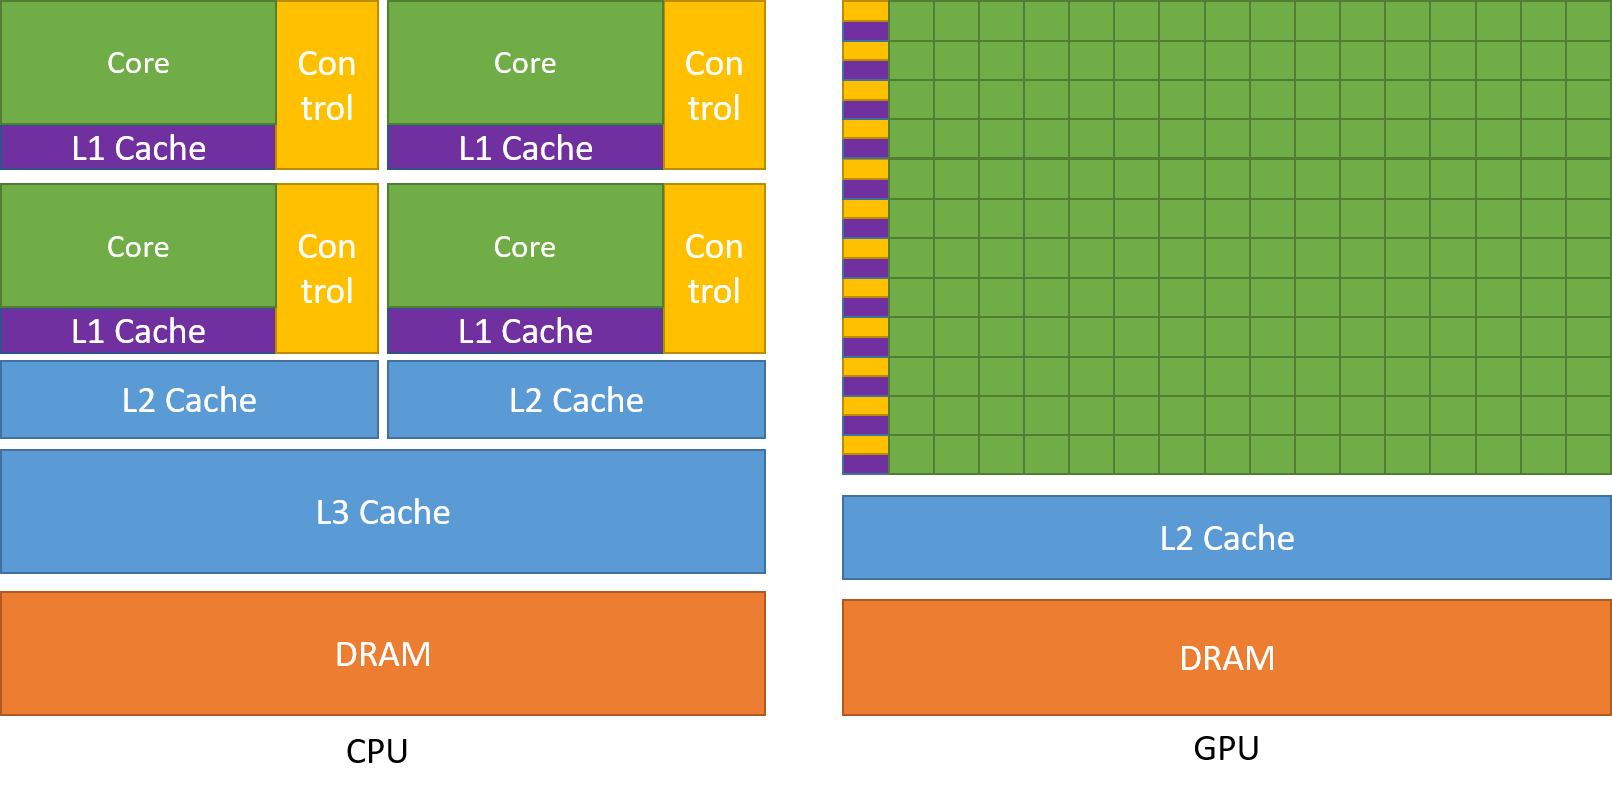
\includegraphics[width=0.8\textwidth]{Chapter_graphics_processing_units/media/gpu-devotes-more-transistors-to-data-processing}
	\caption{\Acrshort{acr:CPU} and \acrshort{acr:GPU} architecture~\cite{Nvidia2021}: \acrshortpl{acr:GPU} dedicate more space to data processing}\label{fig:cpu_gpu}
\end{figure}

Graphics processing units and central processing units are fundamentally made up of the same core
components. First, data processing hardware, shown in green on Figure~\ref{fig:cpu_gpu}, consists of
the parts of the chips that do calculations on data. Control flow hardware, shown in yellow,
schedules instructions to be executed on processing hardware. In orange is the main memory of either
architecture. Main memory or \textit{\acrfull{acr:DRAM}}, shown in orange, stores data to be used
for computations. The main memory very big, and takes a relatively long time to access. Finally, in
blue and purple are different levels of cache memory. Cache is much smaller and much faster than
main memory, and as such stores parts of the memory that the processing hardware is actively using
in order to speed up access.

The two architectures differ as to the balance between the size and capacities of these components.
Chip area is limited by the processes used to manufacture them, so the different components must
share this limited space, and sacrifices must be made. \Acrshortpl{acr:GPU} dedicate much more space
to data processing, increasing throughput. Their compute units are also smaller, to work on more
data in parallel. \Acrshortpl{acr:CPU}, on the other hand, have fewer bigger compute units with a
higher clock speed in order to reduce latency. Their compute units are called cores. The
\acrshort{acr:GPU} compute units are called \acrshort{acr:CUDA} cores, and are arranged in rows as
\textit{\acrfullpl{acr:SM}}.

In order to reduce latency, \acrshortpl{acr:CPU} have a lot of die space dedicated to cache. More
cache helps keep data close in access time. More data is loaded from main memory at a time, assuming
that data that is near needed data will also be needed later. The deeper hierarchy of cache of
\acrshortpl{acr:CPU} helps keep the cores working on the current problem as fast as possible, never
starving for memory. \Acrshortpl{acr:GPU} have less total cache and fewer levels of cache to make
room for more \acrshort{acr:CUDA} cores. As a throughput oriented device, it is less important how
fast individual tasks complete, as long as more tasks overall are completed. The reduced cache is
acceptable because if a \acrshort{acr:CUDA} core is waiting on data from the main memory that was
not found in cache, it will simply pause execution of that thread and execute another thread. On
\acrshortpl{acr:GPU}, the smallest and fastest cache, L1 cache, is shared within a
\acrshort{acr:SM}. It is thus fast to access shared data, as long as conflicts are avoided.

Finally, \acrshortpl{acr:CPU} also reduce latency by using much more potent control flow units.
Firstly, they have one control flow unit per core, where \acrshortpl{acr:GPU} have one control flow
unit per row of cores. This limits how many instructions can be dispatched to the cores making up a
\acrshort{acr:SM}. The cores will therefore execute the same execution at the same time in groups of
32, called warps. This makes branching much more expensive if it happens within a warp. If a part of
a program has two branches, A and B, the cores executing branch A will execute, followed by the
cores executing branch B. These have to be executed sequentially because the control flow unit can
only dispatch one instruction per warp. This multiplies the computation time by the number of taken
branches. \Acrshort{acr:CPU} cores only execute a single branch, or can even execute both branches
at once while waiting for the result of the conditional, keeping only the correct result once the
conditional has been evaluated. The more powerful control flow units of \acrshortpl{acr:CPU} may
also perform branch prediction, consisting of the \acrshort{acr:CPU} guessing the most likely branch
based on the result of previous computations and starting to execute this branch while waiting for
the conditional. All this is performed as an effort to reduce latency as much as possible. Programs
running on \acrshortpl{acr:GPU} must compensate by avoiding divergence as much as possible within
warps.

\subsection{Programming model}\label{subsection:graphics_processing_units:architecture:programming_model}

This work uses the \acrshort{acr:CUDA} programming model. It is a programming language, framework
and runtime developed to enable programming on \acrshortpl{acr:GPU} with an extension of the C++
language. Programs using the language execute on the \acrshort{acr:CPU} like a normal program, but
can schedule parts of the program, called kernels, to be executed on the \acrshort{acr:GPU}. Kernels
are run in parallel on the \acrshort{acr:GPU}, asynchronously from the \acrshort{acr:CPU}. The
\acrshort{acr:CPU} is therefore free to do computations of its own while the \acrshort{acr:GPU} is
executing, including adding more kernels or transfers to the \acrshort{acr:GPU} execution queue.
Multiple such queues, called streams, can exist. The purpose of using multiple streams is to execute
independent computations on the \acrshort{acr:GPU} concurrently, and maximise \acrshort{acr:GPU}
usage in case a stream is waiting. \Acrshortpl{acr:GPU} can concurrently execute kernels, transfer
data from the \acrshort{acr:CPU} to the \acrshort{acr:GPU}, and transfer data from the
\acrshort{acr:GPU} to the \acrshort{acr:CPU}. These transfers are necessary because
\acrshort{acr:CPU} and \acrshort{acr:GPU} main \acrlong{acr:RAM} are separate. This means that data
needed for computations on the \acrshort{acr:GPU} that cannot be generated on it must be explicitly
transferred from the \acrshort{acr:CPU}, and results living on the \acrshort{acr:GPU} must be
transferred back to the \acrshort{acr:CPU} in order to be displayed or written to disk. As
\acrshortpl{acr:GPU} are also generally running the displays of non-server computers, results that
are only meant to be viewed can be directly displayed and such transfers can be skipped. This is not
the case for this work. 

\begin{figure}[H]
	\centering
	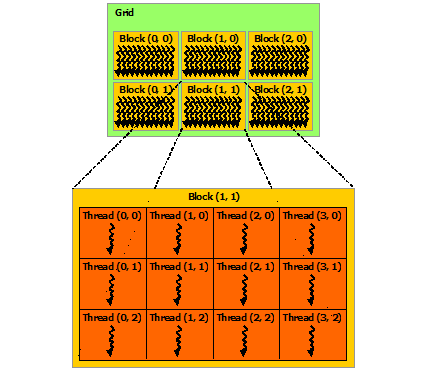
\includegraphics[width=0.6\textwidth]{Chapter_graphics_processing_units/media/grid-of-thread-blocks}
	\caption{\Acrshort{acr:GPU} programming model~\cite{Nvidia2021}: Execution is split into multiple parallelism levels}\label{fig:gpu_programming_model}
\end{figure}

The programing model ties in with the hardware model from
Subsection~\ref{subsection:graphics_processing_units:architecture:hardware_model} by decomposing the
execution of kernels to multiple parallel levels. A kernel will be executed in parallel, with each
core executing the same function. Figure~\ref{fig:gpu_programming_model} shows how programming model
decomposes a problem. The whole problem to be solved is represented as a multidimensional grid of
tasks, with two dimensions in this example. The kernel will execute until the whole grid has been
computed. The grid is broken up into blocks of threads. The different blocks will be dispatched to
the \acrlongpl{acr:SM} of the \acrshort{acr:GPU}, and each thread of that block will be executed on
a \acrshort{acr:CUDA} core of the \acrshort{acr:SM}. A \acrshort{acr:SM} can execute multiple blocks
at the same time if there are more cores within the \acrshort{acr:SM} than threads within a block.
Blocks need to be completely independent of each other, as they cannot be synchronised and may
execute in any order. They also cannot share local memory, as each \acrshort{acr:SM} has its own L1
cache. Threads within the same block can depend on one another, as they are executed concurrently on
the same \acrshort{acr:SM}. Threads from a block execute the same instruction at the same time in
groups of 32, or warps. This is the \textit{\acrfull{acr:SIMT}} architecture. If there are more
threads within a block than cores within a \acrshort{acr:SM}, warps will be run sequentially until
all threads are done with the instruction. Threads within a block can share local memory, and
synchronise with each other. This is useful for algorithms with steps like reductions, where threads
will wait until all threads have computed one level of the reduction, to use the result of that
level for the next one.

Typical execution of a program that adds an array A to an array B and stores the result in an array
C will proceed as follows. The \acrshort{acr:CPU} side of the program will create two arrays of data
in its memory, and initialise them as needed. It will then create two arrays of the same size on the
\acrshort{acr:GPU} using the \acrshort{acr:CUDA} runtime, and transfer the data from the
\acrshort{acr:CPU} arrays A and B to the \acrshort{acr:GPU} arrays. It will then create a result
array C on the \acrshort{acr:GPU}, and one on the \acrshort{acr:CPU}. It will then launch a kernel
on the \acrshort{acr:GPU}, with pointers to the \acrshort{acr:GPU} A and B arrays, and the
\acrshort{acr:GPU} C array. The number of elements in the vectors will dictate the size of the
execution grid. The number of elements will be split in blocks of threads of fixed size, for example
blocks of 128 threads. The number and size of blocks is given to the \acrshort{acr:GPU} when calling
the kernel. The \acrshort{acr:CPU} then must wait until the computation is done using a
synchronisation with the \acrshort{acr:CUDA} runtime, transfer the data from the \acrshort{acr:GPU}
C array to the \acrshort{acr:CPU} C array, and display the results. 

This model fits well with many \acrshort{acr:CFD} methods, including the \acrshort{acr:DG-SEM} used
in this work. We work on a mesh made up of elements and faces connecting them. Elements are
independent during most of the computation and their computations can be executed in parallel. The
only step from the main solver loop needing extra care is the computation of the fluxes between the
elements. The flux computation uses the data from the elements on either side of a face, computes a
flux and stores that flux back in both elements so they can compute their derivative. Since there
can be multiple faces on each side of an element as detailed in
Section~\ref{section:adaptive_mesh_refinement:mortar_element_method}, and each element has multiple
sides, multiple threads will attempt to read and write to the same locations at the same time. This
is a race condition, where the result of the computation will be dependent on the order in which the
threads will try to access the memory location. The results may also be wrong. If two threads read a
value, add their contribution, and store the value, only whichever thread wrote its result last will
have its contributed accounted for in the final result. Different approaches are possible to solve
this issue. For example, Giuliani and Krivodonova~\cite{Giuliani2019} use an edge colouring method
where the same kernel is run multiple times on different edges in order to avoir writing to the
elements at the same time. Our program parallelises this part of the computation on the faces
connecting the elements instead, as described in
Section~\ref{section:spectral_element_method:implementation}. As long as there are enough elements
in the mesh to saturate the cores of the \acrshort{acr:GPU} with work, this part of the program
should be efficient to run on the \acrshort{acr:GPU}.

The adaptivity and load balancing algorithms shown in
Chapters~\ref{chapter:adaptive_mesh_refinement} and~\ref{chapter:load_balancing} are not so easily
parallelisable. These algorithms are sequential in nature, with many operations needing the result
of previous ones to complete their calculations. In order to parallelise them, a few support
structures have to be added for the different processing threads to be able to find the data they
have been assigned, and the different memory locations they are allowed to access. Another issue is
that a kernel operating on certain objects, elements for example, should not modify other objects,
such as faces. This is done to avoid race conditions when multiple threads try to access the same
memory location, faces in this example. The practical consequence of this is that objects moving to
a new index in their storage arrays cannot update their neighbour faces to point to their new index.
Their neighbours must therefore have the required information to compute where the element will move
when the face moves itself, and update the index itself. By designing the algorithms this way, a
kernel running on an object type will have each thread writing to only a single object corresponding
to its index, avoiding race conditions. More information on how the algorithms are designed is
available in
Sections~\ref{section:spectral_element_method:implementation},~\ref{section:adaptive_mesh_refinement:implementation}
and~\ref{section:load_balancing:implementation}.

The meshes generated by \acrlong{acr:AMR} and dynamic load balancing are also not naturally suited
for \acrshortpl{acr:GPU}. These processors are more suited for static repetitive tasks. Element
splitting, changing their polynomial order and moving elements around will reduce the efficiency of
the computations if care is not taken to tune the algorithms to this platform. Different polynomial
orders elements in a thread warp will introduce branching, and the warp will take as much time to
execute as the highest polynomial order elements. Moving and splitting elements will put more
pressure on the limited cache of \acrshortpl{acr:GPU}, as threads will loop on different elements
after refinement and load balancing. The interval between each refinement and load balancing will
have to be tuned to trade off between having an optimal mesh for computations and having a static
mesh for more iterations.

\section{Process Parallelism}\label{section:graphics_processing_units:process_parallelism}

When trying to solve very large problems, a single node with a single \acrshort{acr:GPU} will have
insufficient processing power and memory to solve the problem in a reasonable time, or at all. To
work with these larger problems, the work needs to be split at another level than \acrshort{acr:GPU}
parallelism.  

The program can use multi-block meshes, with each block being worked on by one process and one
\acrshort{acr:GPU}. If there are fewer \acrshortpl{acr:GPU} available on a system than there are
processes, some processes will share a single \acrshort{acr:GPU} by using asynchronous execution
streams. The different processes communicate together using \textit{\acrfull{acr:MPI}} at their
boundaries. Since the solution data resides on the \acrshort{acr:GPU}, it must first be copied to
the main \acrshort{acr:CPU} memory before it is sent through the \acrshort{acr:MPI} runtime. It then
needs to be copied to the receiving process' \acrshort{acr:GPU}. This exchange necessitates multiple
transfers on different levels and should be optimised as much as possible. An approach to minimise
the number of interfaces between the different mesh blocks is explained in
Chapter~\ref{chapter:load_balancing}. 

It is possible to split the mesh into more blocks than there are \acrshortpl{acr:GPU} in a system.
In this case, there will be one process per block, and some processes will share
\acrshortpl{acr:GPU}. The \acrshortpl{acr:GPU} will be split into virtual partitions, using
concurrent execution streams. These streams execute concurrently on a \acrshort{acr:GPU}, leveraging
the fact that some operations can happen at the same time, up to one running kernel, one transfer
from the \acrshort{acr:CPU} to the \acrshort{acr:GPU}, and one transfer from the \acrshort{acr:GPU}
to the \acrshort{acr:CPU}. Additionally, the \acrshort{acr:GPU} can execute one kernel while another
kernel is waiting for memory. These partitions do not increase performance, but are useful to test
running more blocks than there are available \acrshortpl{acr:GPU}, or running the program with a
mesh that is split into more blocks than available \acrshortpl{acr:GPU} without re-splitting it.

A simple mesh generator program and a mesh partitioner are available as part of this work. The mesh
generator can create square meshes of arbitrary resolution with different boundary conditions. The
mesh partitioner can split arbitrary single block meshes to multi-block meshes.

These tasks, each consisting of a mesh block, do not necessarily need to run on
\acrshortpl{acr:GPU}. A \acrshort{acr:CPU} version of the program is provided to compare the
efficiency of the program and to aid debugging. That version uses \acrshort{acr:CPU} workers doing
the same computations. The program could even be modified to dispatch work to \acrshort{acr:CPU} and
\acrshort{acr:GPU} workers to use the full computing power of a system. Some work would need to be
done to ascertain the relative capacity of the different workers, as a \acrshort{acr:GPU} worker
running on a complete \acrshort{acr:GPU} is much faster than a \acrshort{acr:CPU} worker running on
a single \acrshort{acr:CPU} core. \Acrshort{acr:CPU} workers could also use multiple threads, with
an architecture similar to the \acrshort{acr:GPU} one.

\section{Data structure}\label{section:graphics_processing_units:data_structure}

The data structure used in this work has been designed to provide good performance on the
\acrshort{acr:GPU} architecture, while keeping the ease of use and programming of \acrshort{acr:CPU}
code. The mesh is unstructured, made up of elements, faces and nodes.
Figure~\ref{fig:mesh_structure} shows the different components of a two block mesh.

\begin{figure}[H]
	\centering
	\subfloat[First mesh block]
	{\includesvg[height=0.55\textwidth]{Chapter_graphics_processing_units/media/mesh_0_after0_P2}\label{fig:mesh_left}}
	\hfill
	\subfloat[Second mesh block]
	{\includesvg[height=0.55\textwidth]{Chapter_graphics_processing_units/media/mesh_1_after0_P2}\label{fig:mesh_right}}
	\caption{Data structure: A mesh split into two blocks (a) First block (b) Second block}\label{fig:mesh_structure}
\end{figure}

\subsection{Performance}\label{subsection:graphics_processing_units:data_structure:performance}

In order to get good performance and fit naturally with the \acrshort{acr:GPU} architecture, the
different objects are stored as flat one-dimensional arrays on the \acrshort{acr:GPU}. The
\acrshort{acr:CUDA} memory allocation functions are run on the \acrshort{acr:CPU} and return a
continuous block of memory on the \acrshort{acr:GPU}, and the memory transfers between the
\acrshort{acr:CPU} and \acrshort{acr:GPU} copy continuous blocks of memory. This matches well with
having flat arrays of objects. Other data structures, like trees, would need multiple memory
allocations from the \acrshort{acr:CPU} and a kernel to assemble them in some kind of structure.
This would be manageable for a non-adaptive solver as it would be performed once, but with mesh
refinement and load balancing the mesh changes constantly. With arrays, an array of the new size is
allocated and the objects are moved to it. Thanks to the structure from
Subsection~\ref{subsection:graphics_processing_units:data_structure:ease_of_programming}, the
elements themselves have a known constant size regardless of polynomial order, and have the bulk of
their size out of the element object, making them fast to move and making the element array smaller.
The flat arrays also reduce indirection and structure the memory accesses. Threads from a kernel
executing on elements directly access the element at their thread index in the element array.

This simplifies greatly transfers between the \acrshort{acr:CPU} and \acrshort{acr:GPU}, and mesh
reallocation when refining or load balancing. On the other hand, it carries less context on the
relation between mesh blocks, complicating the element exchanges from
Chapter~\ref{chapter:load_balancing}. It also means that elements and faces move around in the
arrays as more are added, and their indices must be updated in other objects linking to them. 

Some data needs to be transferred to the \acrshort{acr:CPU} during the computation, such as fluxes
between mesh blocks in different processes, and data to be written to the output files. These
transfers use arrays allocated on the \acrshort{acr:CPU} and \acrshort{acr:GPU}, and a kernel
storing the data into the \acrshort{acr:GPU} array. The array can then be transferred to the
\acrshort{acr:CPU}, and either written to disk or sent to another \acrshort{acr:CPU} and then its
\acrshort{acr:GPU}.

\subsection{Ease of use}\label{subsection:graphics_processing_units:data_structure:ease_of_use}

\begin{figure}[H]
	\centering
	\subfloat[Structured mesh]
	{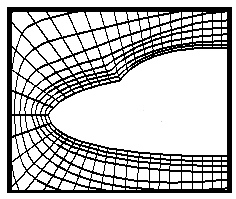
\includegraphics[width=0.45\textwidth]{Chapter_graphics_processing_units/media/structured_mesh}\label{fig:structured_mesh}}
	\hfill
	\subfloat[Unstructured mesh]
	{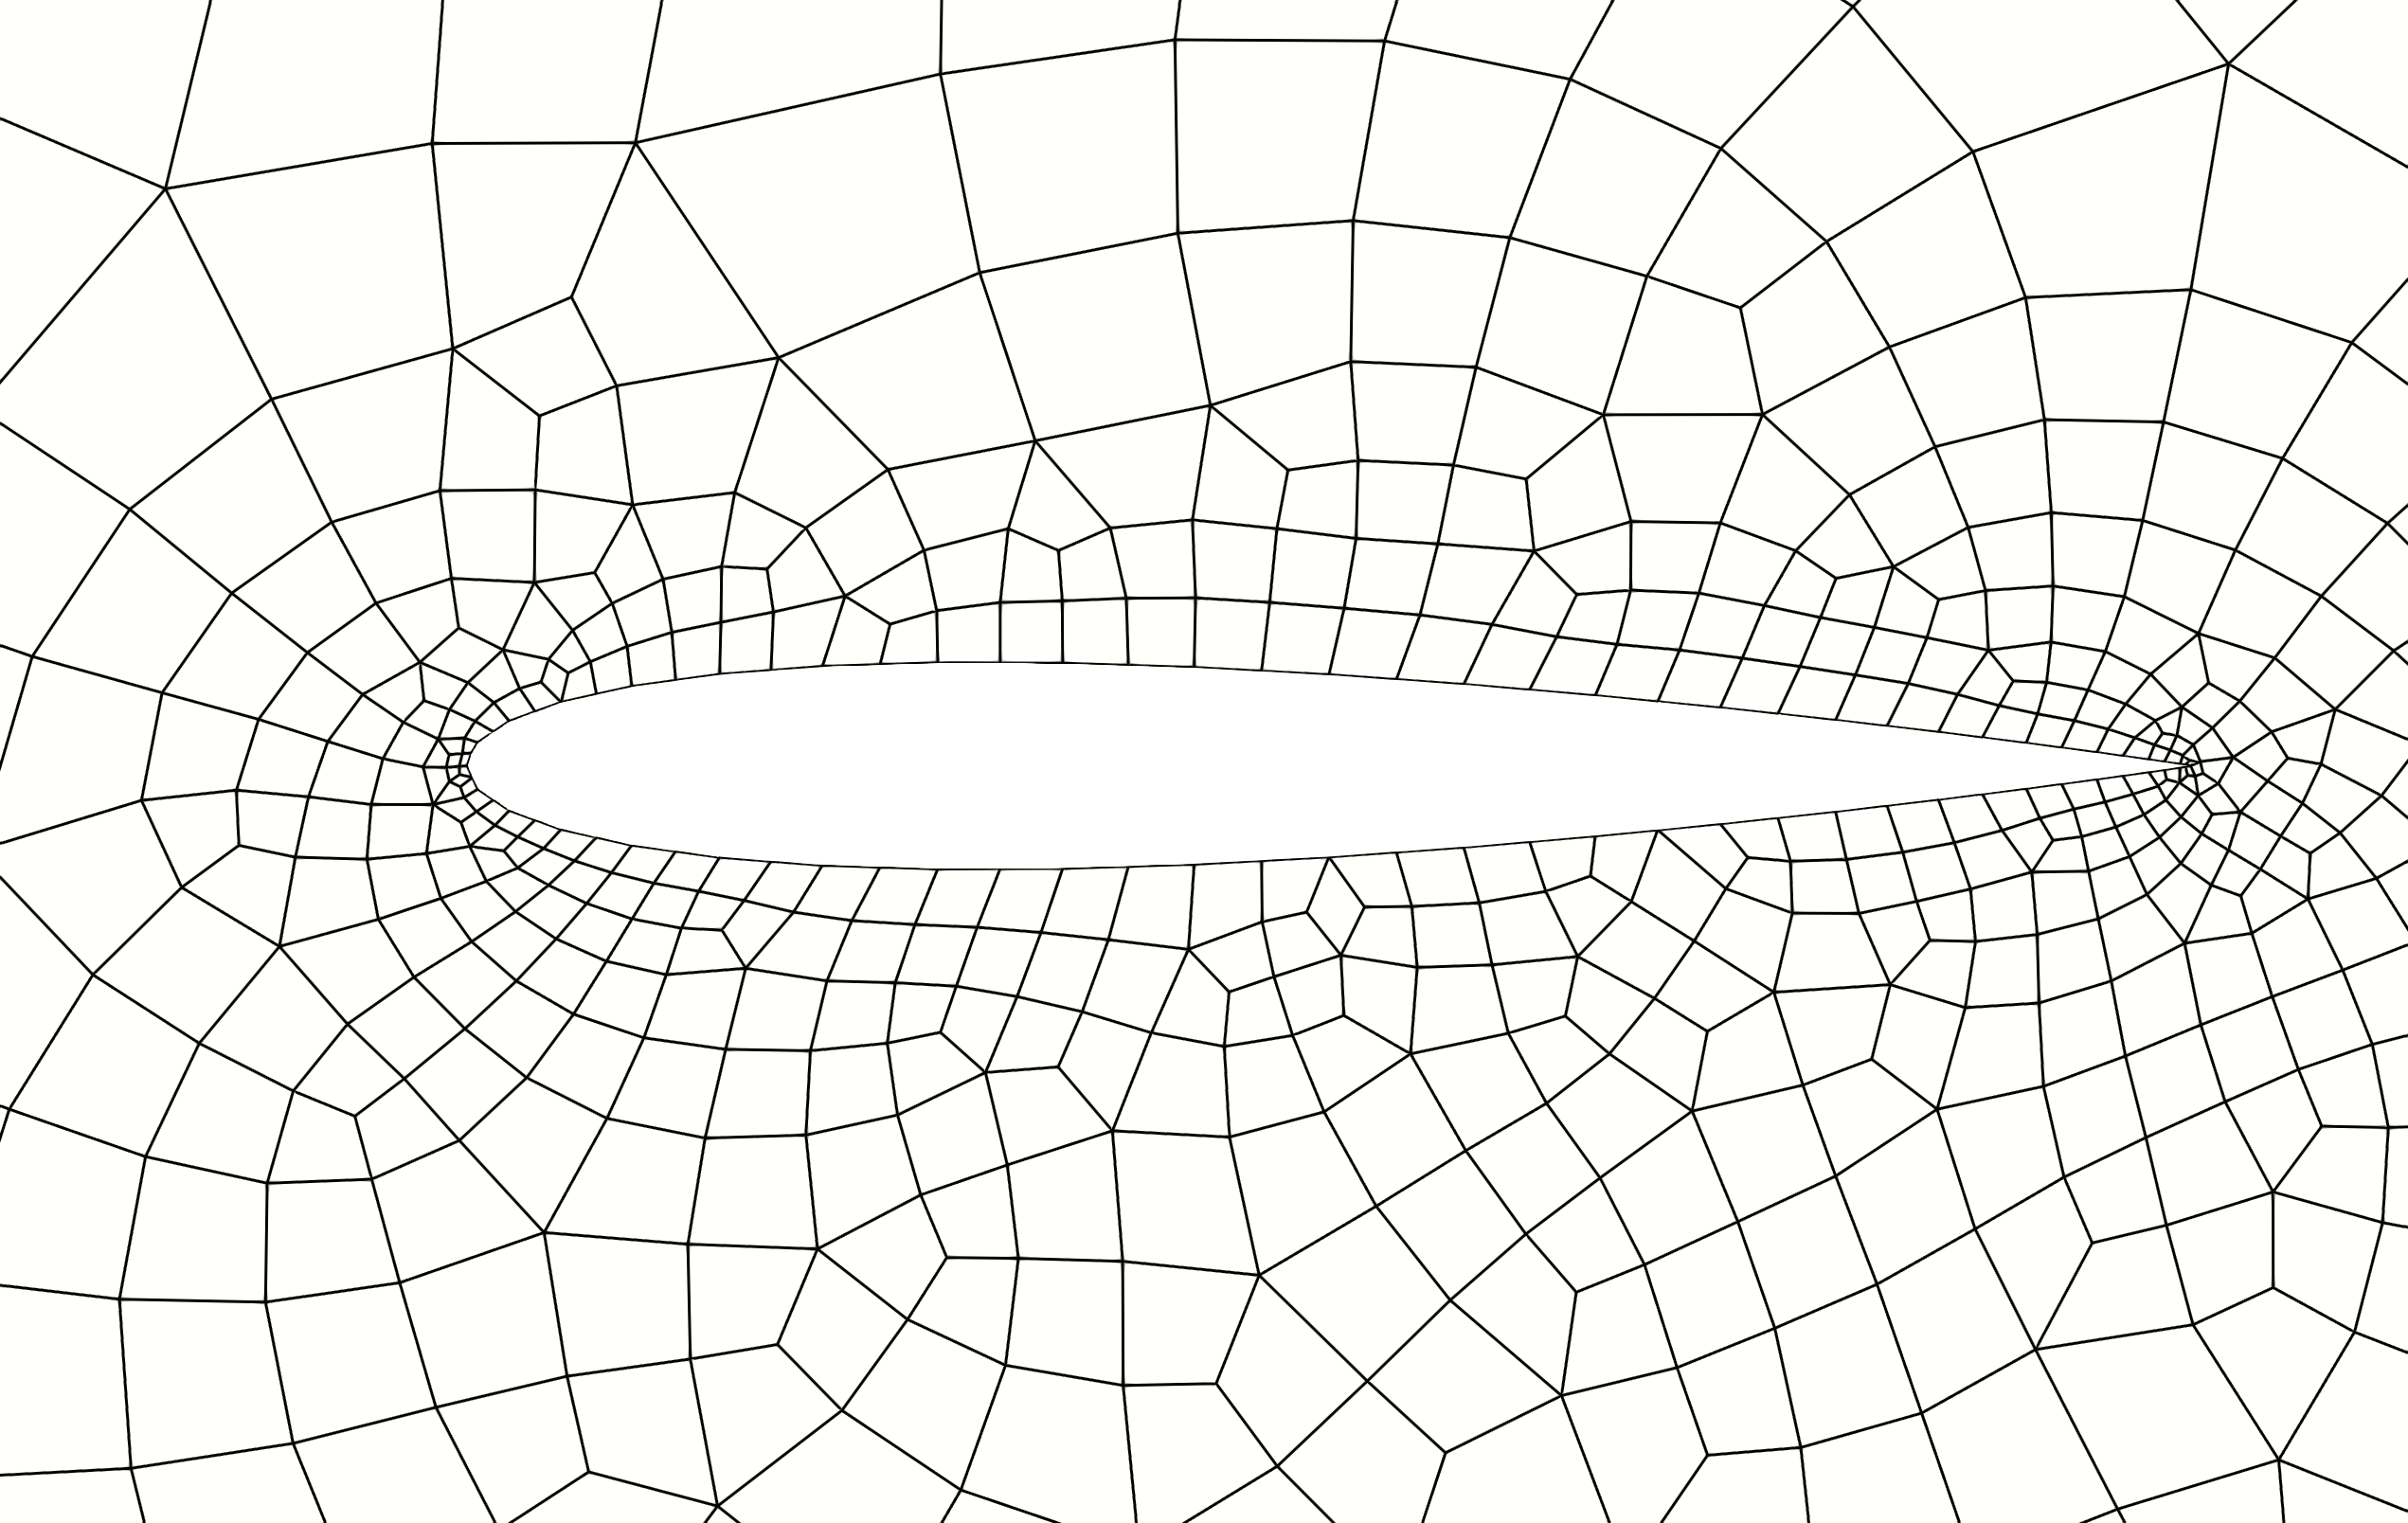
\includegraphics[width=0.45\textwidth]{Chapter_graphics_processing_units/media/unstructured_mesh}\label{fig:unstructured_mesh}}
	\caption{Types of meshes~\cite{Clucas1999}: (a) Structured (b) Unstructured}\label{fig:mesh_types}
\end{figure}

In order to increase ease of use, the program is made to work with unstructured meshes. Unstructured
meshes allow for increased flexibility when meshing, and an unstructured mesh solver can easily be
made to also read structured meshes. In unstructured meshes, elements are not necessarily numbered
in any order. Elements hold an explicit list of the indices of their neighbours. In structured
meshes, elements are placed in a regular grid, and have an index describing their location. In 2D,
this is the row and column of the element. The neighbours of an element are found by simply
incrementing or decrementing the index.

\begin{figure}[H]
	\centering
	\subfloat[Structured mesh]
	{\includesvg[width=0.5\textwidth]{Chapter_graphics_processing_units/media/structured_memory}\label{fig:structured_memory}}
	\hfill
	\subfloat[Unstructured mesh]
	{\includesvg[width=0.5\textwidth]{Chapter_graphics_processing_units/media/unstructured_memory}\label{fig:unstructured_memory}}
	\caption{Memory accesses: (a) Structured (b) Unstructured}\label{fig:mesh_memory}
\end{figure}

Here a concession has been made for flexibility, as structured meshes would be faster than
unstructured meshes on a \acrshort{acr:GPU}. Threads on a \acrshort{acr:GPU} benefit from accessing
memory in an ordered fashion. With a structured mesh, thread warps need only one memory access to
obtain all their neighbours. The neighbours are packed in memory, and their index can be computed
easily by incrementing the element indices. For unstructured meshes, neighbour indices have to be
fetched from an area in memory, and the neighbours are not guaranteed to be contiguous in memory.
This adds an indirection, and may need multiple memory accesses.

Since unstructured meshes enable more complex meshes to be represented than strictly regular
quadrilaterals, this tradeoff is accepted, and acts as a worst case scenario for the performance of
\acrshortpl{acr:GPU}.

The program uses the \textit{\acrfull{acr:CGNS}} mesh format. Both the provided mesh generator and mesh partitioner output
the format, and the mesh partitioner and solver can read the format. The format is widely used,
which should enable this program to read the many already available meshes using the format.

The program outputs data using the \textit{\acrfull{acr:VTK}} format. Once again, this is a widely
used format, notably used by the \textit{ParaView} visualisation application. The results of the
program should then be easy to manipulate and display.

\subsection{Ease of programming}\label{subsection:graphics_processing_units:data_structure:ease_of_programming}

The program is written partly using the Object-oriented paradigm, especially for the data structure
part. Elements, faces and nodes are objects, each with multiple data members and methods. This
groups many parameters together that would be separate arrays otherwise, making it easier to program
and keep track of the different members of objects. This has the disadvantage of putting more
pressure on the limited cache of \acrshortpl{acr:GPU}, and potentially increase the number of memory
accesses needed. This is the structure of arrays against array of structures debate. It increases
cache pressure when a loop only accesses a subset of the data members of an object. For example, the
solution update function only uses the solution and derivative of an element. When threads loop over
those elements, they have to load entire elements into cache. If the solution and derivative were
stored into separate arrays, many more elements could fit in cache as only their solution and
derivative would be fetched. This would also improve memory accesses, as warps of threads would need
fewer memory accesses since the data is continuous.

On the other hand, using objects simplifies many parts of the code. Elements can be sent and
received from process to process as a whole: adding a data member doesn't necessitate modifying
every part of the code that copies or creates elements. This is especially useful as we can use
constructors and destructors for objects.

\begin{figure}[H]
	\centering
	\includesvg[width=0.6\textwidth]{Chapter_graphics_processing_units/media/moving_elements}
	\caption{Moving elements: The data stored in dynamic memory does not need to be copied}\label{fig:moving_elements}
\end{figure}

Constructors and destructors are used here because the objects use dynamic memory for their solution
data. As elements and faces can have a different polynomial order, they need to store more or less
data depending on the polynomial order. This makes it impossible to create an array of objects,
unless all objects use the maximum size they can have, negating the memory advantage of lower-order
elements. Instead, in this work objects use dynamic memory to hold their variable size arrays. They
hold pointers to that memory, making the objects themselves fixed in size. This has the added
benefit of making the objects smaller and easier to move around, as only the pointers and the
geometry data have to be moved while the bigger solution data stays in dynamic memory. 

Unlike the main arrays which are allocated from the \acrshort{acr:CPU} on the \acrshort{acr:GPU}
using the \acrshort{acr:CUDA} runtime, \acrshort{acr:GPU} dynamic memory is allocated on the
\acrshort{acr:GPU} itself. When the elements are created in a kernel, each thread will allocate
memory in parallel in the object constructor. That memory will be deallocated when the element is
deleted. Coupled with move semantics of modern C++, this allows an automatic management of that
memory on the \acrshort{acr:GPU}, similar to how we would use smart pointers or arrays in usual C++.
Dynamic memory allocation on the \acrshort{acr:GPU} is a relatively new feature, which enables
programming patterns closer to those used for \acrshort{acr:CPU} programming.

\section{Implementation}\label{section:graphics_processing_units:implementation}
% Talk about reduce operations, data transfers for boundaries

\subsection{Kernels}\label{subsection:graphics_processing_units:implementation:kernels}

\subsection{Reductions}\label{subsection:graphics_processing_units:implementation:reductions}

Reductions are operations that are difficult to make efficient and parallel on \acrshortpl{acr:GPU}.
Harris et al.~\cite{Harris2007} show a few different ways to optimise these operations. In this
work, we need to compute the minimum time step over the whole mesh at every time step. This
operation uses geometric and solution data from the elements to find each element's minimum time
step size. This data is only available on the \acrshort{acr:GPU}. 

\begin{figure}[H]
	\centering
	\includesvg[width=0.45\textwidth]{Chapter_graphics_processing_units/media/reduction}
	\caption{Reduction: A block of threads compute the minimum of data}\label{fig:reduction}
\end{figure}

An implementation must saturate the \acrshort{acr:GPU} with work as much as possible: blindly
looping one thread over the whole mesh will only use one of the approximately five thousand cores of
the \acrshort{acr:GPU}, for one thousandth of the speed. 

\subsection{MPI transfers}\label{subsection:graphics_processing_units:implementation:mpi_transfers}


    % spectral element method
    \chapter{Discontinuous Galerkin Spectral Element Method} \label{chapter:spectral_element_method} 
% Talk about non-conform interfaces here?
% Cite Kopriva

\section{Spectral approximation} \label{section:spectral_element_method:spectral_approximation}
% Legendre polynomials, both forms
% Polynomial interpolation

\section{Equation} \label{section:spectral_element_method:equation}

\section{DG-SEM} \label{section:spectral_element_method:dg_sem}

\section{Implementation} \label{section:spectral_element_method:implementation}
% Talk about the flux computation, possible race conditions


    % adaptive mesh refinement
    \chapter{Adaptive Mesh Refinement} \label{chapter:adaptive_mesh_refinement} 
% Something about move semantics
% No coarsening
% Adaptivity triggers

    % load balancing
    \chapter{Load Balancing} \label{chapter:load_balancing} 
% Hilbert curve
% Hilbert state "guess"
% MPI transfers
% Non-conforming boundaries
% Reconstruction
% Say it only uses number of elements, point to results for N influence on GPUs
% Talk about load imbalance



    % results
    \chapter{Results}\label{chapter:results}

This chapter presents results of the implementation of the adaptive \acrshort{acr:DG-SEM} wave
equation solver on \acrshort{acr:GPU} architectures and studies its effectiveness. Three main
components are studied. First, the performance of the core spectral element method code on
\acrshortpl{acr:GPU} is presented in Section~\ref{section:results:scaling_tests} with a comparison
with the same code running on \acrshortpl{acr:CPU} for a simple wave problem. Then, the performance
of the \acrlong{acr:AMR} is studied in Section~\ref{section:results:adaptivity_performance}. Dynamic
load balancing is studied in Section~\ref{section:results:load_balancing_performance}. Finally, more
complex applications are shown in Sections~\ref{section:results:complex_application}
and~\ref{section:results:complex_meshes}.

\section{Platforms}\label{section:results:platforms}

The implementation we have developed aims to perform large scale computations, and as such targets
\acrshort{acr:HPC} platforms. The program has been designed to scale to multiple levels of
parallelism, the highest being splitting the workload between several \acrshort{acr:HPC} nodes, each
having multiple \acrshortpl{acr:CPU} and \acrshortpl{acr:GPU}. To showcase how the program works on
such platforms, most of the following tests were run on clusters graciously offered by Compute
Canada\footnote{https://www.computecanada.ca/}. Two such clusters were used for our experiments,
Béluga and Narval.

\subsection{Béluga}\label{subsection:results:platforms:beluga}

Béluga is a heterogeneous cluster suitable for a variety of purposes, from traditional
\acrshort{acr:CPU} computing to massively parallel \acrshort{acr:GPU} computing. It is located at
the École de technologie supérieure in Montréal. Béluga is made up of 977 compute nodes of different
types, totaling 39,120 \acrshort{acr:CPU} cores and 696 \acrshortpl{acr:GPU}. For our testing, we
use Béluga's general usage \acrshort{acr:GPU} nodes. Each one of the 172 \acrshort{acr:GPU} nodes
contains 40 \acrshort{acr:CPU} cores and 186 GB of memory across two Intel Gold 6148
\acrshortpl{acr:CPU}, and four Nvidia V100 SXM2 \acrshortpl{acr:GPU} with 16 GB of memory each. One
such node totals about 2 TFlops of double precision \acrshort{acr:CPU} computing power, and 13
TFlops of double precision \acrshort{acr:GPU} computing power. The nodes are connected by Infiniband
HDR (100 Gb/s) interconnections.

\subsection{Narval}\label{subsection:results:platforms:narval}

Narval is a heterogeneous cluster suitable for a variety of purposes, from traditional
\acrshort{acr:CPU} computing to massively parallel \acrshort{acr:GPU} computing and artificial
intelligence workloads. It is also located at École de technologie supérieure in Montréal. Narval is
made up of 1301 compute nodes of different types, totaling 80,720 \acrshort{acr:CPU} cores and 636
\acrshortpl{acr:GPU}. For our testing, we use Narval's \acrshort{acr:GPU} nodes. Each one of the 159
\acrshort{acr:GPU} nodes contains 48 \acrshort{acr:CPU} cores and 498 GB of memory across two AMD
Milan 7413 \acrshortpl{acr:CPU}, and four Nvidia A100 \acrshortpl{acr:GPU} with 40 GB of memory
each. One such node totals about 2.2 TFlops of double precision \acrshort{acr:CPU} computing power,
and 38.8 TFlops of double precision \acrshort{acr:GPU} computing power. The nodes are connected by
Infiniband EDR (100 Gb/s) interconnections.

\subsection{Consumer hardware}\label{subsection:results:platforms:consumer}

Some smaller scale tests or tests that did not involve performance were run on consumer hardware.
This is important, as it may not always be possible to access \acrshort{acr:HPC} systems when flow
simulations have to be performed. The program should also have reasonable performance on regular
systems. The system used in these cases is a single computer containing 16 \acrshort{acr:CPU} cores
and 128 GB of memory across two Intel E5\textendash2650 V2 \acrshortpl{acr:CPU}, and one Nvidia GTX
1070 \acrshort{acr:GPU} with 8 GB of memory. This totals about 0.5 TFlops of double precision
\acrshort{acr:CPU} computing power, and 0.25 TFlops of double precision \acrshort{acr:GPU} computing
power. This is an interesting comparison, as consumer \acrshortpl{acr:GPU} are not geared towards
high precision compute loads. \Acrshortpl{acr:GPU} found in \acrshort{acr:HPC} systems typically
have a 1:2 ratio between their double precision and single precision performance, whereas consumer
\acrshortpl{acr:GPU} usually have 1:32 ratio. This means that computations using double precision
floating point numbers will execute at one sixteenth of the speed of compute-oriented
\acrshortpl{acr:GPU}, all other factors being equal.

\section{Test Case}\label{section:results:test_case}

The test case used in this chapter is shown in Figure~\ref{fig:problem}. We solve the 2D wave
equation from Section~\ref{section:spectral_element_method:equation} on a square domain of size 1 in
each dimension. A linear wave starts just outside of the domain, and traverses the domain
diagonally. Figure~\ref{fig:problem} shows the pressure distribution at \(0.5 s\). The number of
elements \( K \) varies depending on the problem, as does the polynomial order \( N \). This problem
should help demonstrate key aspects of the program, as the solution is steeper near the wave and
needs refinement for accurate results.

\begin{figure}[H]
    \centering
    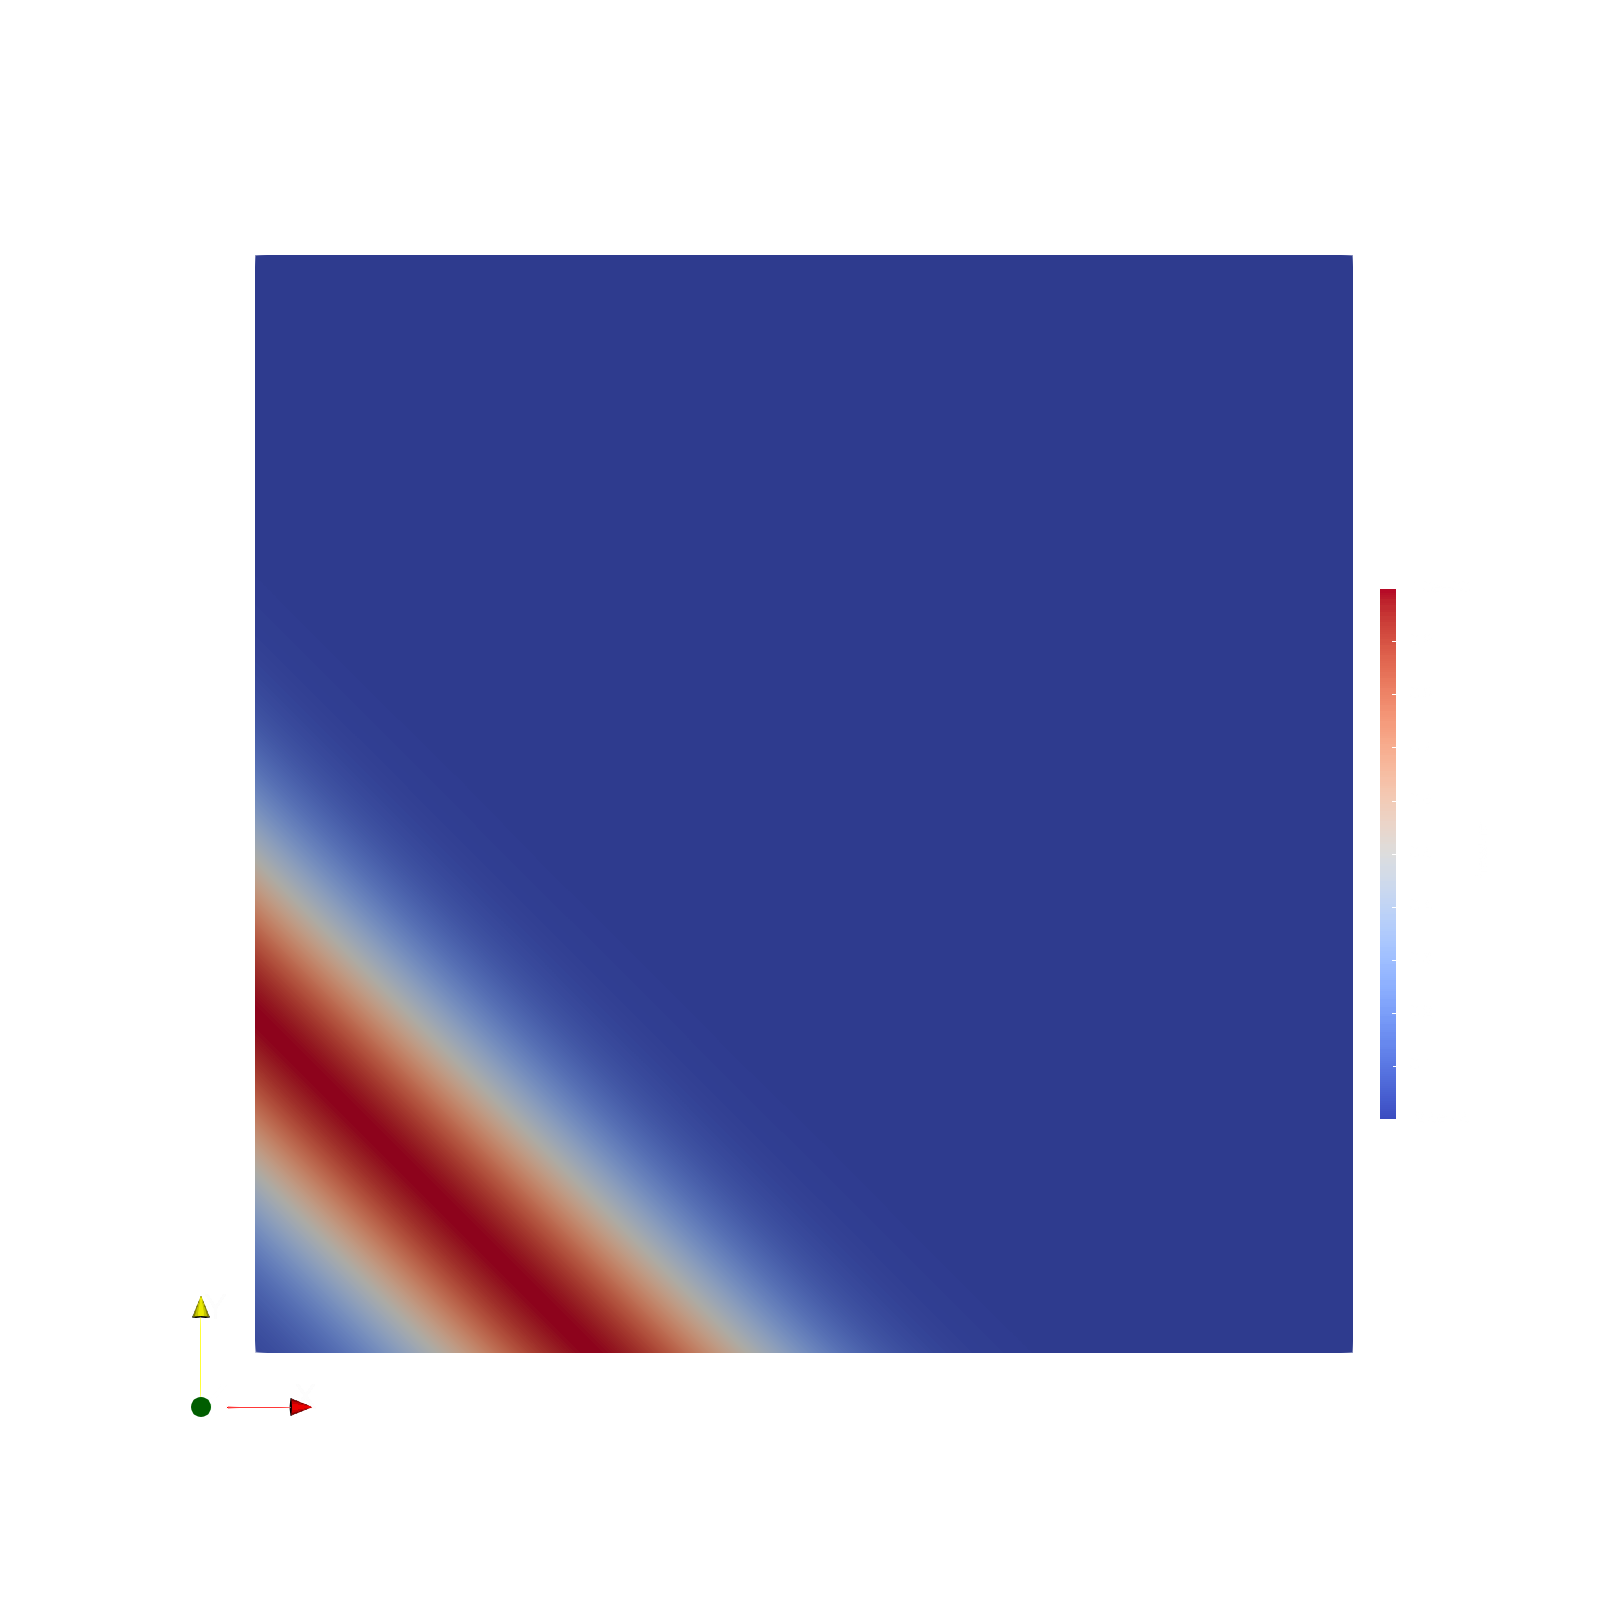
\includegraphics[width=0.6\textwidth]{Chapter_results/media/problem_1}
    \caption{Test case: A wave travels through a square domain at a 45° angle.}\label{fig:problem}
\end{figure}

\section{Scaling Tests}\label{section:results:scaling_tests}

Parallel scaling is an important aspect of the performance of a program. It describes how the
execution time varies when more resources are assigned to the problem. This is an optimisation
problem, as each problem will need a different amount of resources dedicated to it to attain the
best scaling possible. 

A completely parallelisable program, often called embarrassingly parallel, should scale linearly
with the amount of resources. The speedup \(S\) of a workload split between \(P\) workers should be
equal to the number of workers in Equation~\ref{equ:scaling}, with \(t_1\) being the time to solve
the problem serially using a single worker, and \(t_p\) being the time to solve the problem in
parallel using \(P\) workers. In this work, workers are a single \acrshort{acr:GPU} or a single
\acrshort{acr:CPU} core for comparative tests.

\begin{equation} \label{equ:scaling}
    S = \frac{t_1}{t_P}
\end{equation}

Unfortunately, it is often not possible to make a program entirely parallel. In such cases, dividing
a problem into more and more smaller tasks obeys the well-known Amdahl's law~\cite{Amdahl1967}, as
seen in Equation~\ref{equ:strong_scaling}. It splits the program into a sequential part \(s\) and a
parallel part \(l\), with only the parallel part scaling with the number of workers.

\begin{equation} \label{equ:strong_scaling}
    S = \frac{1}{s + \frac{l}{P}}
\end{equation}

This is called \textit{strong scaling}, where a fixed problem is solved using varying amount of
resources. Results of strong scaling tests of the solver are discussed in
Subsection~\ref{subsection:results:scaling_tests:strong}.

On the other hand, increased available resources can enable working on bigger problems. Gustafson
argues that modern highly parallel computers will be used to solve more complex problems instead of
solving smaller problems faster. Such a scaling is described with Equation~\ref{equ:weak_scaling}.

\begin{equation} \label{equ:weak_scaling}
    S = s + l \times P
\end{equation}

This is called \textit{weak scaling}. It describes solving a problem whose size increases with the
amount of resources, while the task size per worker stays constant. Weak scaling is tested in
Subsection~\ref{subsection:results:scaling_tests:weak}. With weak scaling a program will scale
indefinitely, with the slope of the scaling being influenced by the parallel proportion of the task.

This section will also serve as a general comparison between performance of the code on
\acrshortpl{acr:CPU} and \acrshortpl{acr:GPU}. All scaling tests have been performed on the Béluga
supercomputer. Scaling is evaluated by varying the number of \textit{nodes}, where a node in this
context is a single computer from Béluga, sporting 40 \acrshort{acr:CPU} cores and 4
\acrshortpl{acr:GPU} as stated in Subsection~\ref{subsection:results:platforms:beluga}. The
four-node execution time of those tests therefore represents the program running on 16
\acrshortpl{acr:GPU} or 160 \acrshort{acr:CPU} cores, for the \acrshort{acr:GPU} and
\acrshort{acr:CPU} computations respectively.

Both scaling tests evaluate the core solver part of the program, as the meshes start with enough
elements to have a well resolved solution all along the simulation. The \acrlong{acr:AMR} and
dynamic load balancing subroutines are still enabled. The subroutines still run their evaluation
phases, the error estimation and load imbalance computation respectively, but do not deem the
estimated error and load imbalance high enough to trigger the whole subroutine. 

\subsection{Strong scaling}\label{subsection:results:scaling_tests:strong}

The test case for this section is described in Section~\ref{section:results:test_case}. It is
divided into \(256\) elements in each of the \(x\) and \(y\) directions, for a total of \(K =
65536\) elements. The problem is then solved in parallel using a range of nodes, from one quarter
node to eight nodes. One quarter node contains \(1\) \acrshort{acr:GPU} and \(10\)
\acrshort{acr:CPU} cores, while eight nodes contain \(16\) \acrshortpl{acr:GPU} and \(160\)
\acrshort{acr:CPU} cores. The mesh is split into blocks accordingly, one block per
\acrshort{acr:GPU} or one block per \acrshort{acr:CPU} core. The first test has a polynomial order
\(N = 4\) for all elements, and a block size \(B = 32\). 

The block size, as explained in
Subsection~\ref{subsection:graphics_processing_units:architecture:programming_model}, is the number
of threads in a block of threads. Having a higher block size can speed up execution by reducing the
number of instructions to dispatch by the control flow unit of the \acrshort{acr:GPU}, because the
instructions are dispatched by block of threads. However, if the threads within a block diverge,
having a higher block size can actually lower performance. A single thread diverging will have all
the threads in its block waiting until it is finished, therefore a higher block size will have more
threads stalled when divergence occurs.

We add two ``ideal'' lines both for the \acrshort{acr:GPU} and \acrshort{acr:CPU} calculations.
These lines represent perfect scaling from a data point. The dashed and dotted line represents
perfect scaling from the first data point, one \acrshort{acr:GPU} or \(10\) \acrshort{acr:CPU}
cores. This is equivalent to halving the computation time every time the computing power doubles.
Figure~\ref{fig:strong_scaling_N4_W32} shows that the \acrshort{acr:GPU} curve is always below this
ideal line. As we increase the number of \acrshortpl{acr:GPU}, the performance scales better than
linearly up to a point, and then decreases. We therefore add a second dashed line, which represents
the scaling from the best point, where the computation time multiplied by the number of
\acrshortpl{acr:GPU} is the lowest. This line is more representative, and will be used for the next
figures.

\begin{figure}[H]
    \centering
    \includesvg[width=0.5\textwidth]{Chapter_results/media/strong_scaling_N4_K65536_W32}
    \caption{Strong scaling: The number of workers increases while the problem size stays fixed. \(N
        = 4\), \(K = 65536\), \(B = 32\)}\label{fig:strong_scaling_N4_W32}
\end{figure}

Figure~\ref{fig:strong_scaling_N4_W32} shows that the \acrshort{acr:GPU} implementation, initially
slower than the \acrshort{acr:CPU} implementation, overtakes it when one full node or more is used.
The higher number of nodes show the \acrshort{acr:GPU} implementation to be \(2.9 \times \) faster
that the \acrshort{acr:CPU} implementation.

At low numbers of \acrshortpl{acr:GPU} working on the same problem, the \acrshortpl{acr:GPU} are
more heavily loaded. It is possible that the higher memory usage, or the increased cache eviction
rate lowers the performance of \acrshortpl{acr:GPU} in that regime. With a lower number of elements
being worked on by a \acrshort{acr:GPU}, cache has to be emptied less often to make room for more
elements to use for computations.

At the end of the curve, we see that the scaling is slightly reduced. This could be a hint that the
\acrshortpl{acr:GPU} are not sufficiently loaded for those cases. These \acrshortpl{acr:GPU} have
many \acrshort{acr:CUDA} cores, \(5120\) each in the case of Béluga. If the workload does not saturate
the \acrshort{acr:GPU}, some of those cores will be idle, leading to worse performance. The best
number of elements per \acrshort{acr:GPU} seems to be around \(4096\) for this case.

The next test, shown in Figure~\ref{fig:strong_scaling_N6_W32}, shows the same test case but with an
increased polynomial order of \(N = 6\) for all elements. The rationale is that the
\acrshort{acr:GPU} should spend more time on the computations, since the computations will be
heavier, while spending the same time on the overhead of kernel calls and other housekeeping.

\begin{figure}[H]
    \centering
    \includesvg[width=0.5\textwidth]{Chapter_results/media/strong_scaling_N6_K65536_W32}
    \caption{Strong scaling: The number of workers increases while the problem size stays fixed. \(N
        = 6\), \(K = 65536\), \(B = 32\)}\label{fig:strong_scaling_N6_W32}
\end{figure}

Figure~\ref{fig:strong_scaling_N6_W32} shows that the increased polynomial order has not increased
the performance of the \acrshort{acr:GPU} implementation compared to the \acrshort{acr:CPU}
implementation, rather shifting to the right the crossover point where the \acrshort{acr:GPU}
implementation is faster. It is possible that the reduced relative performance is linked to the
increased memory used by the solution, as the needed storage scales with \({2 N + 1}^2\), where
\(N\) is the polynomial order of elements.

Next, this last case is computed again with increased block size \(B\), first 64 on
Figure~\ref{fig:strong_scaling_N6_W64}, then 128 on Figure~\ref{fig:strong_scaling_N6_W128}. The
\acrshort{acr:CPU} implementation is not modified. This should assess the incidence of block size on
the solution time.

\begin{figure}[H]
    \centering
    \subfloat[\(B = 64\)]
    {\includesvg[width=0.5\textwidth]{Chapter_results/media/strong_scaling_N6_K65536_W64}\label{fig:strong_scaling_N6_W64}}
    \hfill
    \subfloat[\(B = 128\)]
    {\includesvg[width=0.5\textwidth]{Chapter_results/media/strong_scaling_N6_K65536_W128}\label{fig:strong_scaling_N6_W128}}
    \caption{Strong scaling: The number of workers increases while the problem size stays fixed. \(N
        = 6\), \(K = 65536\) (a) \(B = 64\) (b) \(B = 128\)}\label{fig:strong_scaling_N6_W64-128}
\end{figure}

As the last figure suggests, increasing the block size \(B\) does incur a performance penalty. This
is possibly caused by a high amount of thread divergence within blocks. This is consistent with how
the program is written, for example Section~\ref{section:adaptive_mesh_refinement:implementation}
shows how the projection back and forth between the elements and faces has several branching code
paths. A lot of changes in the architecture of the program would have to be made to reduce this
branching, and switch to a more data-driven approach.

One thing to note is that the curve of the \acrshort{acr:CPU} implementation on
Figures~\ref{fig:strong_scaling_N4_W32} and~\ref{fig:strong_scaling_N6_W32} is similar, whereas the
\acrshort{acr:GPU} curves from all the figures differ significantly. This is a recurring theme of
all the tests in this chapter: code running on \acrshortpl{acr:GPU} seems to be harder to optimise
and some factors have unexpected influences on the performance.

\subsection{Weak scaling}\label{subsection:results:scaling_tests:weak}

The weak scaling test uses the test case from Section~\ref{section:results:test_case}. The domain is
split up into elements such that each node contains 16384 elements. This amounts to 4096 elements
per \acrshort{acr:GPU}, or 410 elements per \acrshort{acr:CPU} core. The simulation is first
computed with the highest number of nodes, therefore the smallest elements and time step size. The
\acrshort{acr:CFL} number is adjusted for all other simulations in order to use the same time step
size, therefore the same total number of iterations. An ideal result is a flat curve, indicating
that by increasing the problem size and resources by the same amount, the simulation time stays the
same. The problem is studied from ¼ node to 16 nodes.

\begin{figure}[H]
    \centering
    \includesvg[width=0.6\textwidth]{Chapter_results/media/weak_scaling_N4_K4096_W32}
    \caption{Weak scaling: The problem size increases with the number of workers. \(N = 4\), \(K =
        16384/{node}\)}\label{fig:weak_scaling}
\end{figure}

Figure~\ref{fig:weak_scaling} shows good weak scaling from the \acrshort{acr:GPU} implementation.
Keeping in mind that the quarter node and single node cases have a reduced workload by not having to
do any \acrshort{acr:MPI} communication over the network, and the quarter node \acrshort{acr:GPU}
case has no \acrshort{acr:MPI} communication to do at all, the \acrshort{acr:GPU} curve is
reasonably flat. The \acrshort{acr:CPU} curve is not as good, indicating that there may be a
bottleneck in the communication part of the program. The \acrshort{acr:CPU} implementation has a
much higher number of workers than the \acrshort{acr:GPU} one, \(40\) per node instead of four,
increasing the inter-process communication needed. The slope of the \acrshort{acr:CPU} curve is
about \(0.4\) with respect to the number of \acrshort{acr:CPU} cores. 

\section{Adaptive Mesh Refinement Performance}\label{section:results:adaptivity_performance}

This section establishes the performance of the \acrlong{acr:AMR}. The problem from
Section~\ref{section:results:test_case} is used, initially split into four elements in each of the
\(x\) and \(y\) directions, fora total of \(K = 16\) elements. The initial polynomial order is \(N =
4\). The system is allowed to refine up to a split level \(S = 5\), meaning a cell can split five
times and become \(\frac{1}{32}\) of the size of the original cell, and up to a polynomial order \(N
= 16\). The target error estimate is set to \num{1e-6}, meaning it will refine elements whose
estimated error is greater than that number.

\Acrlong{acr:AMR} is a costly process, as the \acrshort{acr:CPU} must reallocate arrays on the
\acrshort{acr:GPU} for the different objects making up the mesh, and then schedule kernels to move
objects to the new arrays. We test here two strategies to reduce the performance overhead of
\acrlong{acr:AMR}, while reducing error. 

First, \acrlong{acr:AMR} will be performed at a regular interval.
Figures~\ref{fig:adaptivity_efficiency_A5},~\ref{fig:adaptivity_efficiency_A20},~\ref{fig:adaptivity_efficiency_A100}
and~\ref{fig:adaptivity_efficiency_A500} show the results of refining the mesh every \(5\), \(20\),
\(100\) and \(500\) timesteps, respectively.

Secondly, the simulations are performed with an increasing number of refinement pre-condition steps
as described in Section~\ref{section:adaptive_mesh_refinement:pre_conditioning}. The analysis ranges
from no pre-condition step to five steps. The total simulation time is shown in blue. It is the sum
of the time taken up by the pre-condition of the mesh, shown in green, and the computation time to
solve the problem, shown in yellow. 

We compare those simulations to two non-adaptive cases. In the first case, the initial mesh is fully
refined uniformly up to the maximum level attained by the adaptive cases. The mesh is split into
\(128\) elements in each of the \(x\) and \(y\) dimensions, for a total of \(K = 16384\) elements,
with a polynomial order \(N = 10\). This result is shown as a dashed line on the figures. The second
non-adaptive case aims to obtain a maximum error similar to the adaptive case. The mesh is refined
uniformly to \(32\) elements in each of the \(x\) and \(y\) dimensions, for a total of \(K = 1024\)
elements, with a polynomial order \(N = 10\). This case is shown as a dotted line on the figures.
Both the simulation time and the error relative to the analytical solution are plotted. The cases
were computed using the Narval supercomputer on a single \acrshort{acr:GPU}.

\begin{figure}[H]
    \centering
    \subfloat[Solution time]
    {\includesvg[width=0.49\textwidth]{Chapter_results/media/adaptivity_time_N4_K16_A5}\label{fig:adaptivity_efficiency_A5_time}}
    \subfloat[Maximum error]
    {\includesvg[width=0.49\textwidth]{Chapter_results/media/adaptivity_error_N4_K16_A5}\label{fig:adaptivity_efficiency_A5_error}}
    \caption{\Acrlong{acr:AMR} performance: Simulation time and error for increasing number of pre-condition steps. \(N_{initial} = 4\), \(K_{initial} = 16\), \(S = 5\), refinement interval = 5}\label{fig:adaptivity_efficiency_A5}
\end{figure}

\begin{figure}[H]
    \centering
    \subfloat[Solution time]
    {\includesvg[width=0.49\textwidth]{Chapter_results/media/adaptivity_time_N4_K16_A20}\label{fig:adaptivity_efficiency_A20_time}}
    \hfill
    \subfloat[Maximum error]
    {\includesvg[width=0.49\textwidth]{Chapter_results/media/adaptivity_error_N4_K16_A20}\label{fig:adaptivity_efficiency_A20_error}}
    \caption{\Acrlong{acr:AMR} performance: Simulation time and error for increasing number of pre-condition steps. \(N_{initial} = 4\), \(K_{initial} = 16\), \(S = 5\), refinement interval = 20}\label{fig:adaptivity_efficiency_A20}
\end{figure}

\begin{figure}[H]
    \centering
    \subfloat[Solution time]
    {\includesvg[width=0.49\textwidth]{Chapter_results/media/adaptivity_time_N4_K16_A100}\label{fig:adaptivity_efficiency_A100_time}}
    \hfill
    \subfloat[Maximum error]
    {\includesvg[width=0.49\textwidth]{Chapter_results/media/adaptivity_error_N4_K16_A100}\label{fig:adaptivity_efficiency_A100_error}}
    \caption{\Acrlong{acr:AMR} performance: Simulation time and error for increasing number of pre-condition steps. \(N_{initial} = 4\), \(K_{initial} = 16\), \(S = 5\), refinement interval = 100}\label{fig:adaptivity_efficiency_A100}
\end{figure}

\begin{figure}[H]
    \centering
    \subfloat[Solution time]
    {\includesvg[width=0.49\textwidth]{Chapter_results/media/adaptivity_time_N4_K16_A500}\label{fig:adaptivity_efficiency_A500_time}}
    \hfill
    \subfloat[Maximum error]
    {\includesvg[width=0.49\textwidth]{Chapter_results/media/adaptivity_error_N4_K16_A500}\label{fig:adaptivity_efficiency_A500_error}}
    \caption{\Acrlong{acr:AMR} performance: Simulation time and error for increasing number of pre-condition steps. \(N_{initial} = 4\), \(K_{initial} = 16\), \(S = 5\), refinement interval = 500}\label{fig:adaptivity_efficiency_A500}
\end{figure}

From
Figures~\ref{fig:adaptivity_efficiency_A5},~\ref{fig:adaptivity_efficiency_A20},~\ref{fig:adaptivity_efficiency_A100}
and~\ref{fig:adaptivity_efficiency_A500}, we see that this is an optimisation problem, with
tradeoffs between the simulation time and the error generated.

An important part of the error comes from the initial conditions being applied on too coarse a mesh.
Even if the mesh is refined, this error propagates through the domain. Mesh pre-condition, as
described in Section~\ref{section:adaptive_mesh_refinement:pre_conditioning}, aims to alleviate this
problem. Indeed, with enough pre-condition steps all cases converge to an acceptable error. Adding
more pre-condition steps does not improve the results, as the target error estimate of \num{1e-6} is
likely reached.

The fully refined non-adaptive case, shown in dashed lines on
Figures~\ref{fig:adaptivity_efficiency_A5},~\ref{fig:adaptivity_efficiency_A20},~\ref{fig:adaptivity_efficiency_A100}
and~\ref{fig:adaptivity_efficiency_A500}, is prohibitively time consuming to compute. The solution
is well resolved as shown on Figure~\ref{fig:adaptivity_efficiency_A20_error}, with the analytical
solution error being \(19 \times \) smaller than in the adaptive case. On the other hand, it takes
\(22 \times \) as much time to compute. The difference is even more pronounced when the refinement
interval is increased to \(100\), as in Figure~\ref{fig:adaptivity_efficiency_A100_time}, where the
adaptive solution with three to five pre-condition steps is around \(67 \times \) faster, at the
expense of a worse error compared to the \(20\) refinement interval case.

As for the similar maximum error non-adaptive case, shown with dotted lines, the results are closer.
The case with a refinement interval of 20 on Figure~\ref{fig:adaptivity_efficiency_A20} was used to
set the target error for that non-adaptive case. The adaptive case starting from a coarse mesh is
able to reach a similar maximum error and similar computation time when compared to the non-adaptive
case. The other cases also attain the target error estimate of \num{1e-6} while being faster.

The non-adaptive cases are closer to being ideal for the \acrshort{acr:GPU} architecture. The
non-adaptive cases have less thread divergence than the adaptive case. There is a lot more branching
in the adaptive case, with elements having a different polynomial order, non-conforming interfaces,
and different numbers of neighbours. This increased divergence lowers the performance since some
threads are predicated off while others execute an instruction. The memory access patterns of the
non-adaptive cases are also better, for example the different faces connecting to an element are
closer in memory. Threads from a same warp accessing memory that is not contiguous must perform
several memory fetches. The non-adaptive cases play to the strengths of the \acrshortpl{acr:GPU},
yet the adaptive case shows performance improvements. This means that \acrshort{acr:AMR} is worth it
even if the \acrshort{acr:GPU} architecture is not perfectly suited for it, and with improvements to
fit it better it could perform even better. Section~\ref{section:conclusion:future_work} discusses
some improvements to make the program even better suited for the \acrshort{acr:GPU} architecture.

The best number of pre-condition steps seems to be four for this case, as the target error is
reached with all refinement intervals. After this number of steps the solution does not change much
as the target error estimate target is likely reached. We use that number of steps to compare the
effects of different refinement intervals in Figure~\ref{fig:adaptivity_efficiency_C4}.

\begin{figure}[H]
    \centering
    \subfloat[Solution time]
    {\includesvg[width=0.49\textwidth]{Chapter_results/media/adaptivity_time_N4_K16_C4}\label{fig:adaptivity_efficiency_C4_time}}
    \hfill
    \subfloat[Maximum error]
    {\includesvg[width=0.49\textwidth]{Chapter_results/media/adaptivity_error_N4_K16_C4}\label{fig:adaptivity_efficiency_C4_error}}
    \caption{\Acrlong{acr:AMR} performance: Simulation time and error for four pre-condition steps and increasing refinement interval. \(N_{initial} = 4\), \(K_{initial} = 16\), \(S = 5\), pre-condition steps = 4}\label{fig:adaptivity_efficiency_C4}
\end{figure}

Figure~\ref{fig:adaptivity_efficiency_C4} gives a good overview of the \acrshort{acr:AMR}
performance. All refinement intervals attain the target error estimate of \num{1e-6}, and obtain a
real maximum error under \num{1e-6} when compared to the analytical solution. 

It is always faster to use \acrshort{acr:AMR} than to start with a uniform fully refined mesh, and
it is faster to use \acrshort{acr:AMR} than a uniformly refined mesh that has the same maximum
solution error. The adaptive case can refine elements where they are most needed, saving computing
resources.

There is a balance to be made between refining often and spending more time in the
\acrshort{acr:AMR} routine, and refining less often therefore using a less refined mesh for longer.
Section~\ref{section:conclusion:future_work} discusses ideas for alternative approaches to choose
when to refine. In this case it seems that performing \acrshort{acr:AMR} every \(20\) time steps
yields the lowest error, while waiting \(100\) timesteps between refinements yields a faster runtime
at the price of a worse error that still stays below the target error estimate we set.

\section{Dynamic Load Balancing Performance}\label{section:results:load_balancing_performance}

This section is dedicated to benchmarking the dynamic load balancing module of the program in
adaptive cases where varying levels of load imbalance are generated. The sample problem is the same
as described in Section~\ref{section:results:test_case}, except that the domain size is increased
from a size of 1 to 100 in either dimension. The wave stays the same, effectively only staying in
the lower left corner during the program runtime. The program advances the solution to a simulation
time of two seconds. The mesh is split into 128 elements in each of the \(x\) and \(y\) directions,
for a total of \(K = 16384\) elements. The initial polynomial order is \(N = 4\). The problem is
solved using four \acrshort{acr:GPU} nodes from the Narval supercomputer, for a total of \(P = 16\)
\acrshortpl{acr:GPU}. This initially amounts to 1024 elements per \acrshort{acr:GPU}. The mesh is
refined every 20 timesteps. In order to prescribe a different load imbalance for different cases, a
different maximum split level \(S\) is set. This parameter controls how many times an element can
h-refine. Three cases are presented, a low load imbalance case with \(S = 3\) shown in
Figures~\ref{fig:load_imbalance_case_low_p} and~\ref{fig:load_imbalance_case_low_s}, a medium load
imbalance case with \(S = 5\) shown in Figures~\ref{fig:load_imbalance_case_medium_p}
and~\ref{fig:load_imbalance_case_medium_s}, and a high load imbalance case with \(S = 7\) shown in
Figures~\ref{fig:load_imbalance_case_high_p} and~\ref{fig:load_imbalance_case_high_s}. The different
cases are allowed to refine up to their respective maximum split level \(S\), and up to a polynomial
order of \(N = 12\). 

\begin{figure}[H]
    \centering
    \subfloat[Full domain]
    {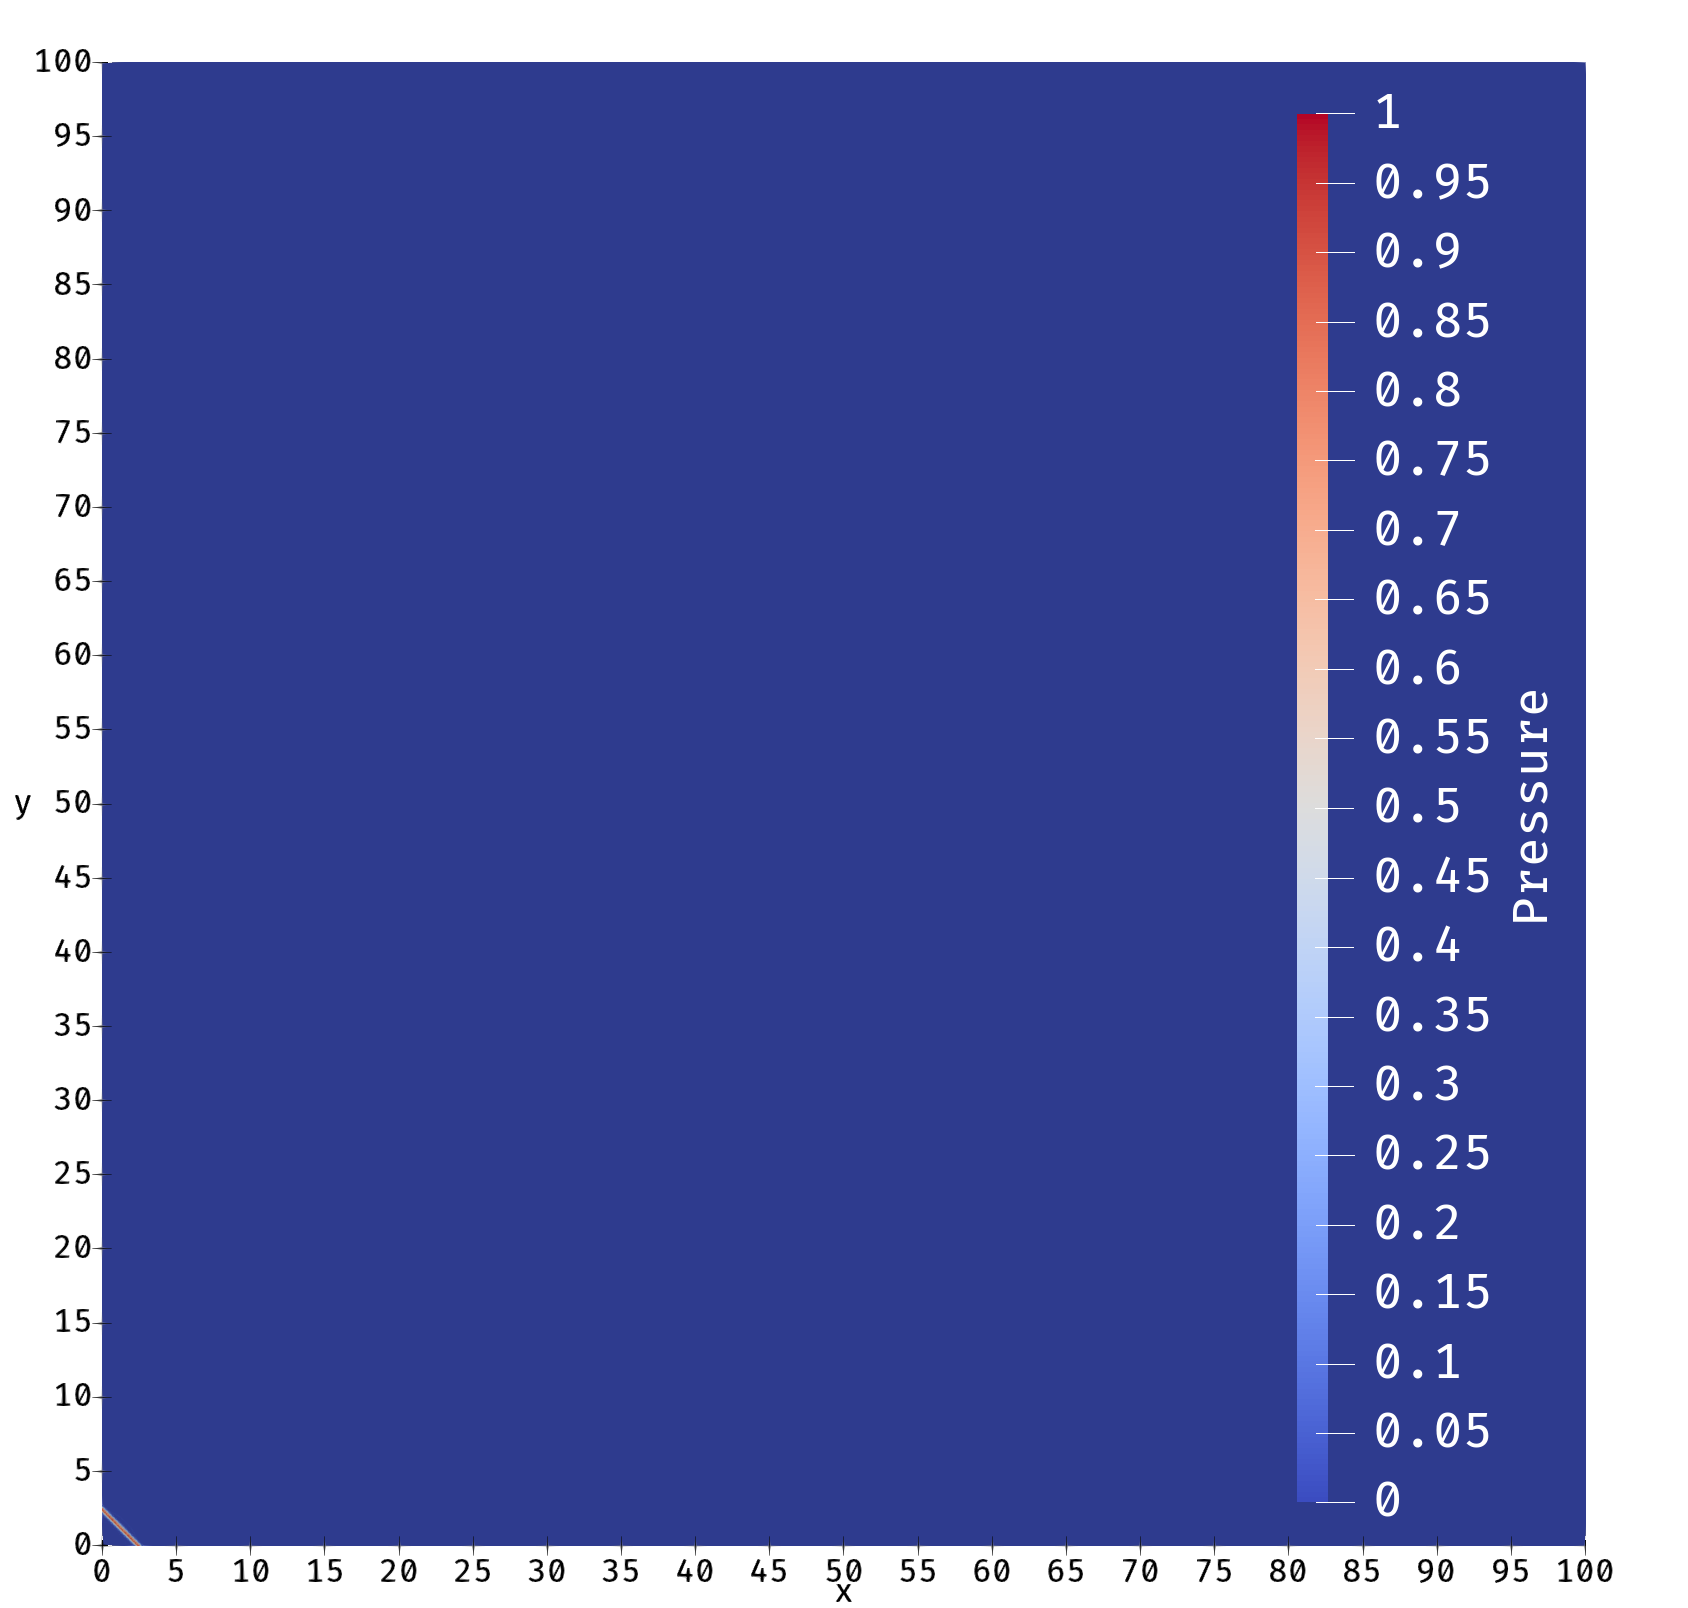
\includegraphics[width=0.5\textwidth]{Chapter_results/media/problem_low_far}\label{fig:load_imbalance_case_low_p_far}}
    \hfill
    \subfloat[Detail]
    {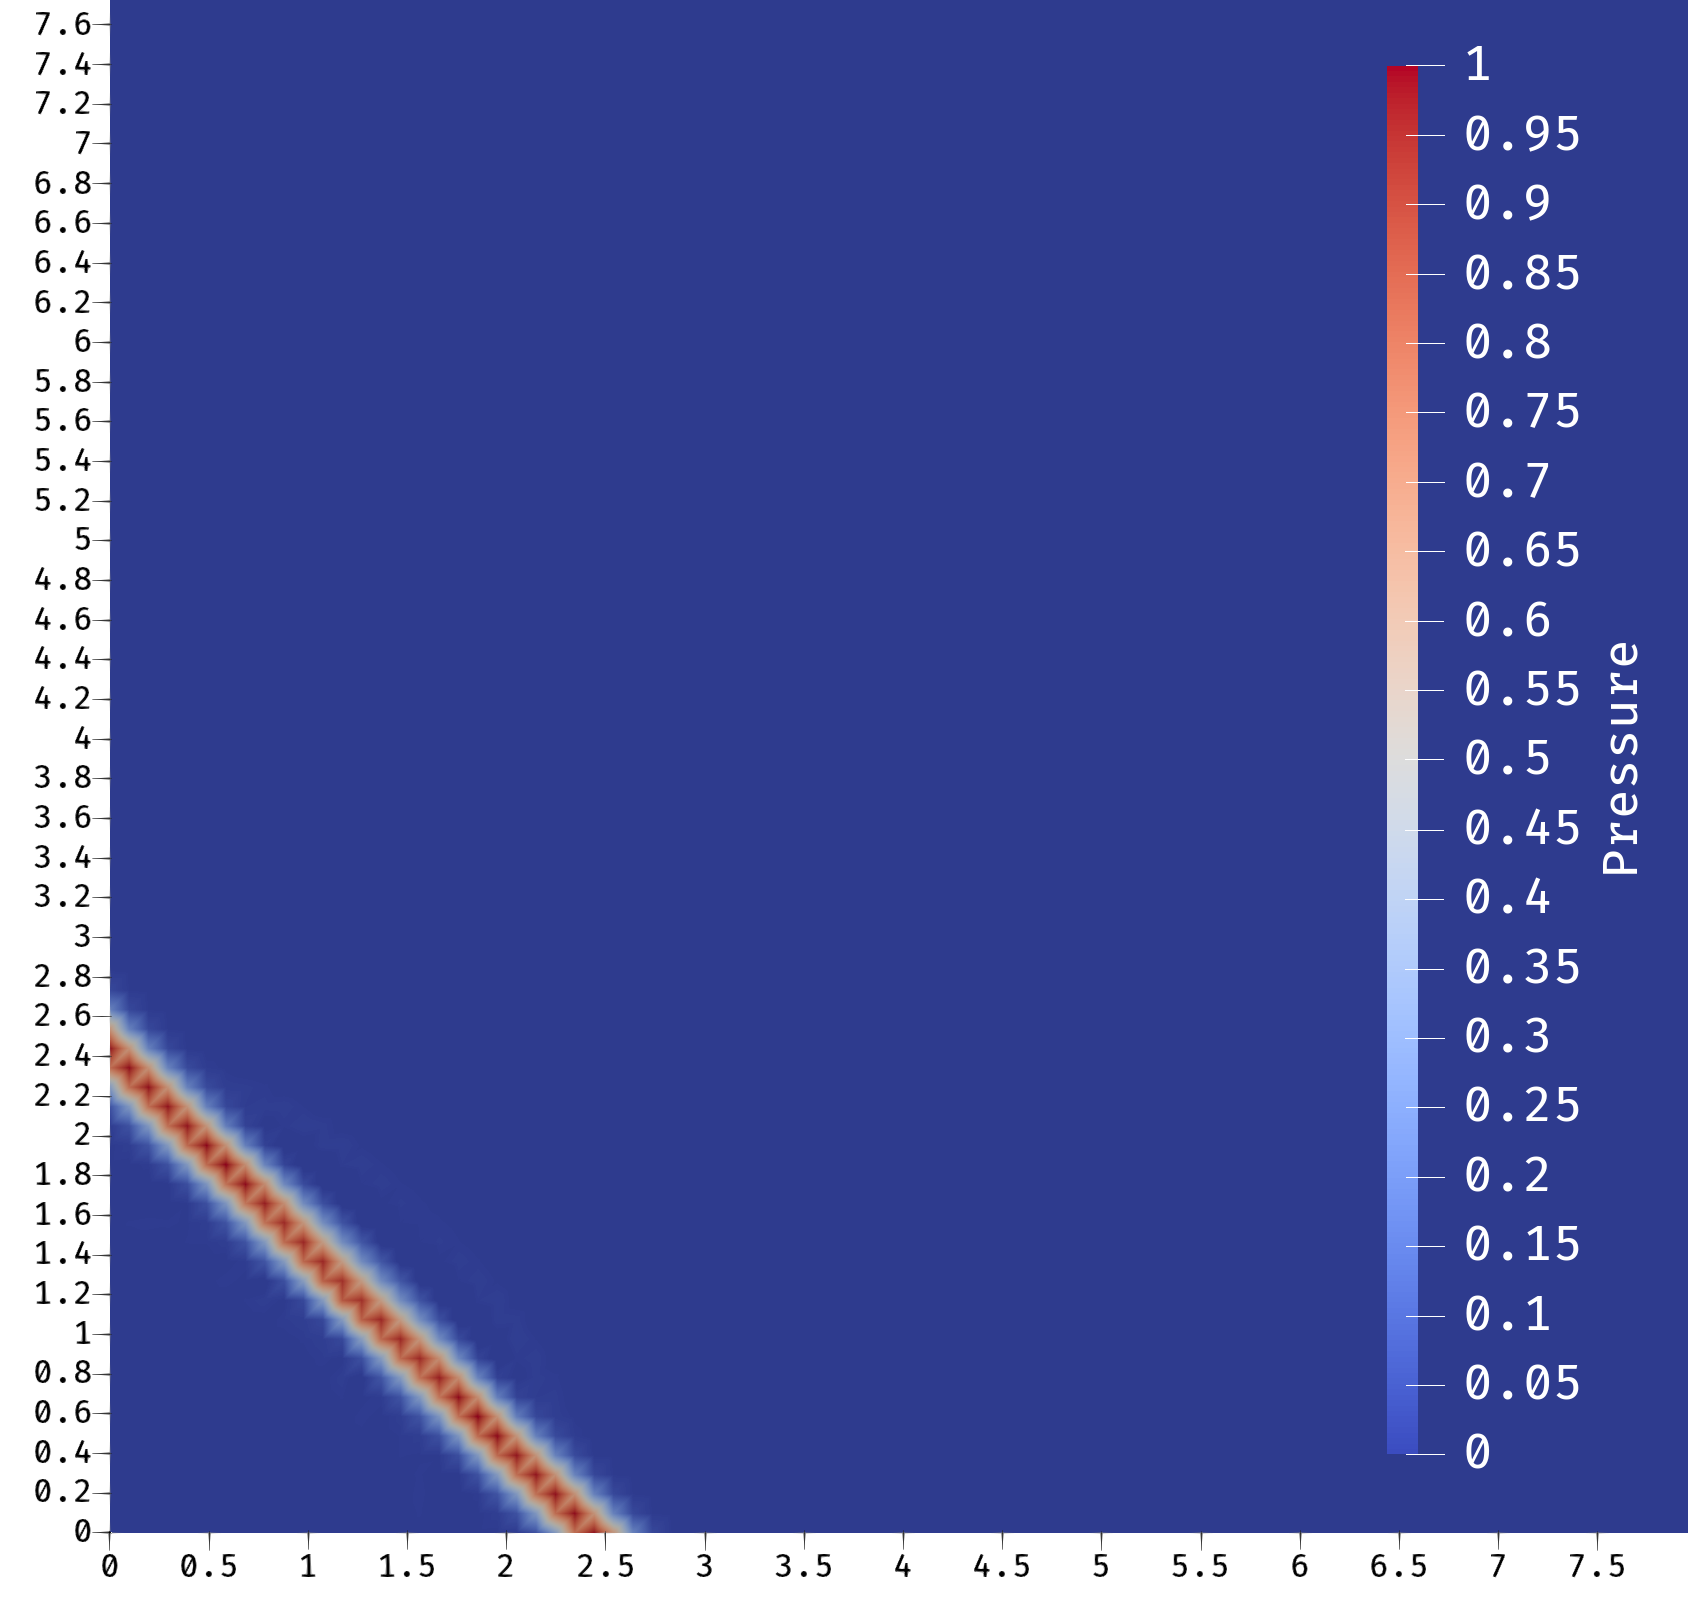
\includegraphics[width=0.48\textwidth]{Chapter_results/media/problem_low_near}\label{fig:load_imbalance_case_low_p_near}}
    \caption{Low load imbalance (\(S = 3\)) test case pressure: A wave passes through a very big domain. \(K_{initial} = 16384\), \(K_{final} = 17752\) (a) Complete domain (b) Area of interest}\label{fig:load_imbalance_case_low_p}
\end{figure}

\begin{figure}[H]
    \centering
    \subfloat[Full domain]
    {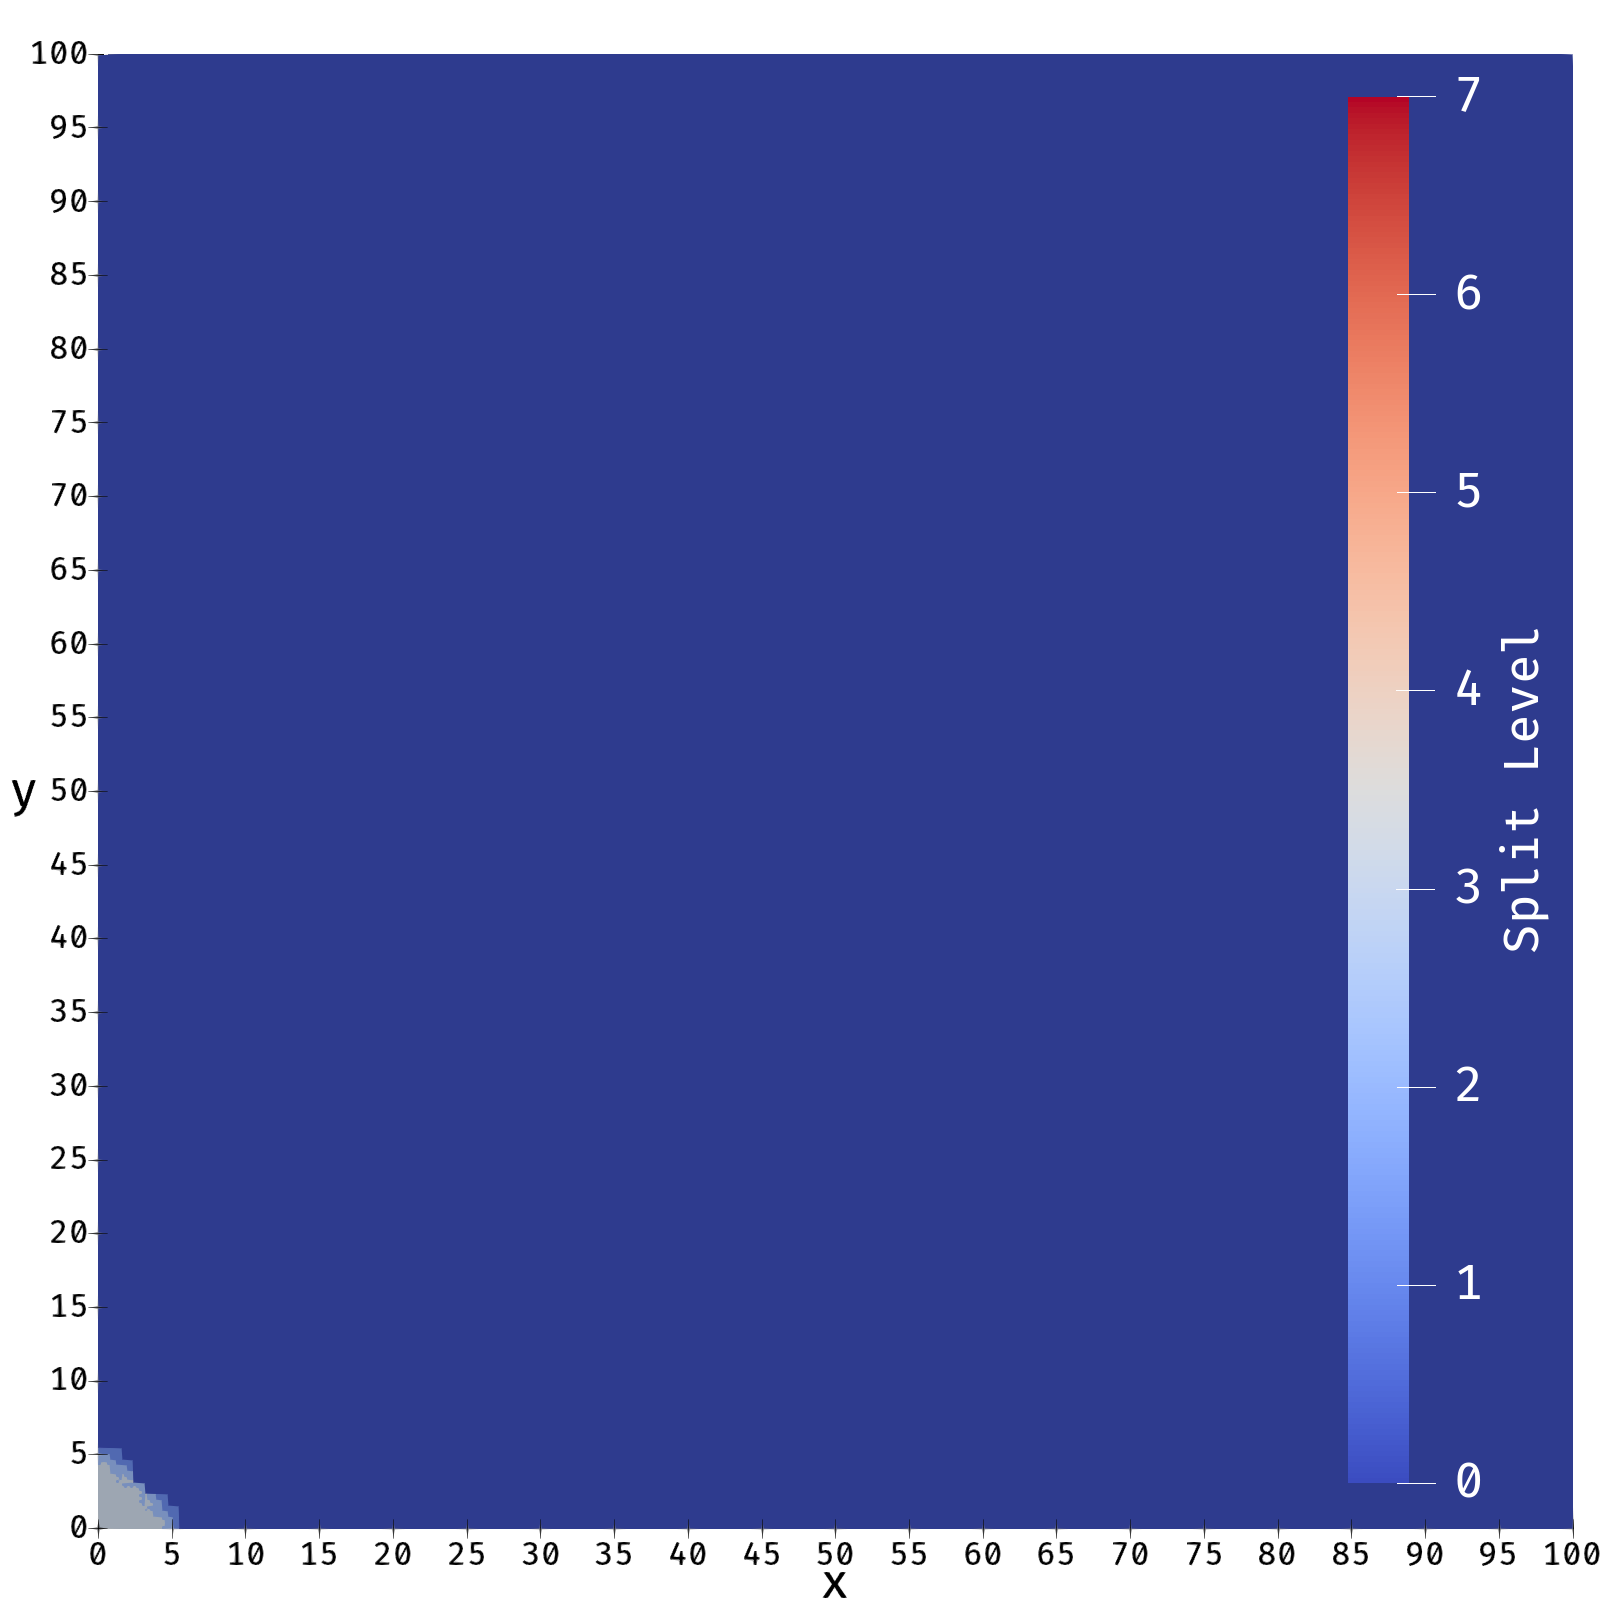
\includegraphics[width=0.5\textwidth]{Chapter_results/media/split_level_low_far}\label{fig:load_imbalance_case_low_s_far}}
    \hfill
    \subfloat[Detail]
    {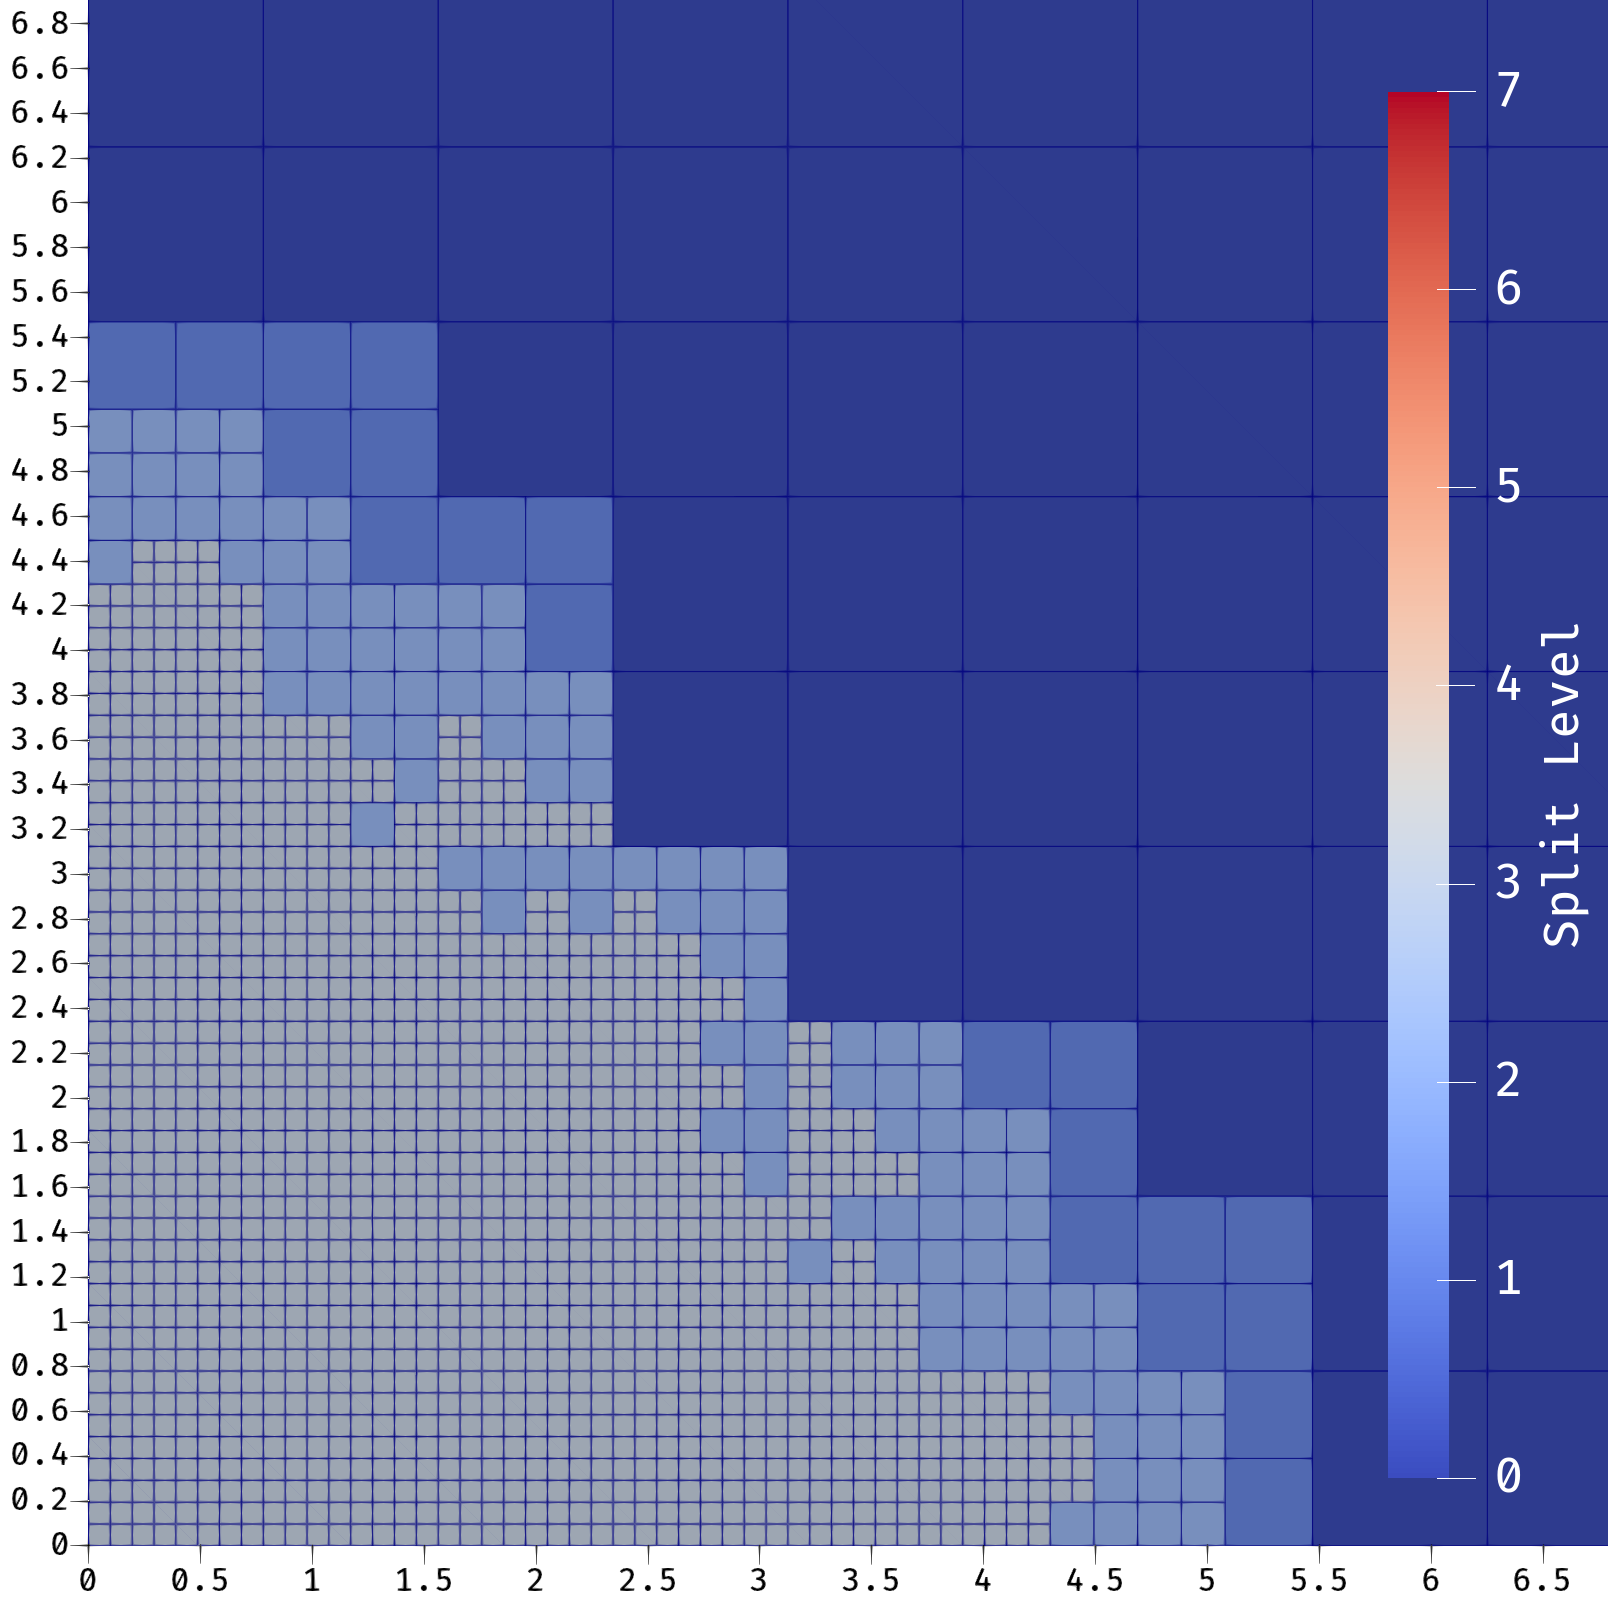
\includegraphics[width=0.48\textwidth]{Chapter_results/media/split_level_low_near}\label{fig:load_imbalance_case_low_s_near}}
    \caption{Low load imbalance (\(S = 3\)) test case split level: Split level, indicating how many times the elements have split, only the bottom left refines. \(K_{initial} = 16384\), \(K_{final} = 17752\) (a) Complete domain (b) Area of interest}\label{fig:load_imbalance_case_low_s}
\end{figure}

\begin{figure}[H]
    \centering
    \subfloat[Full domain]
    {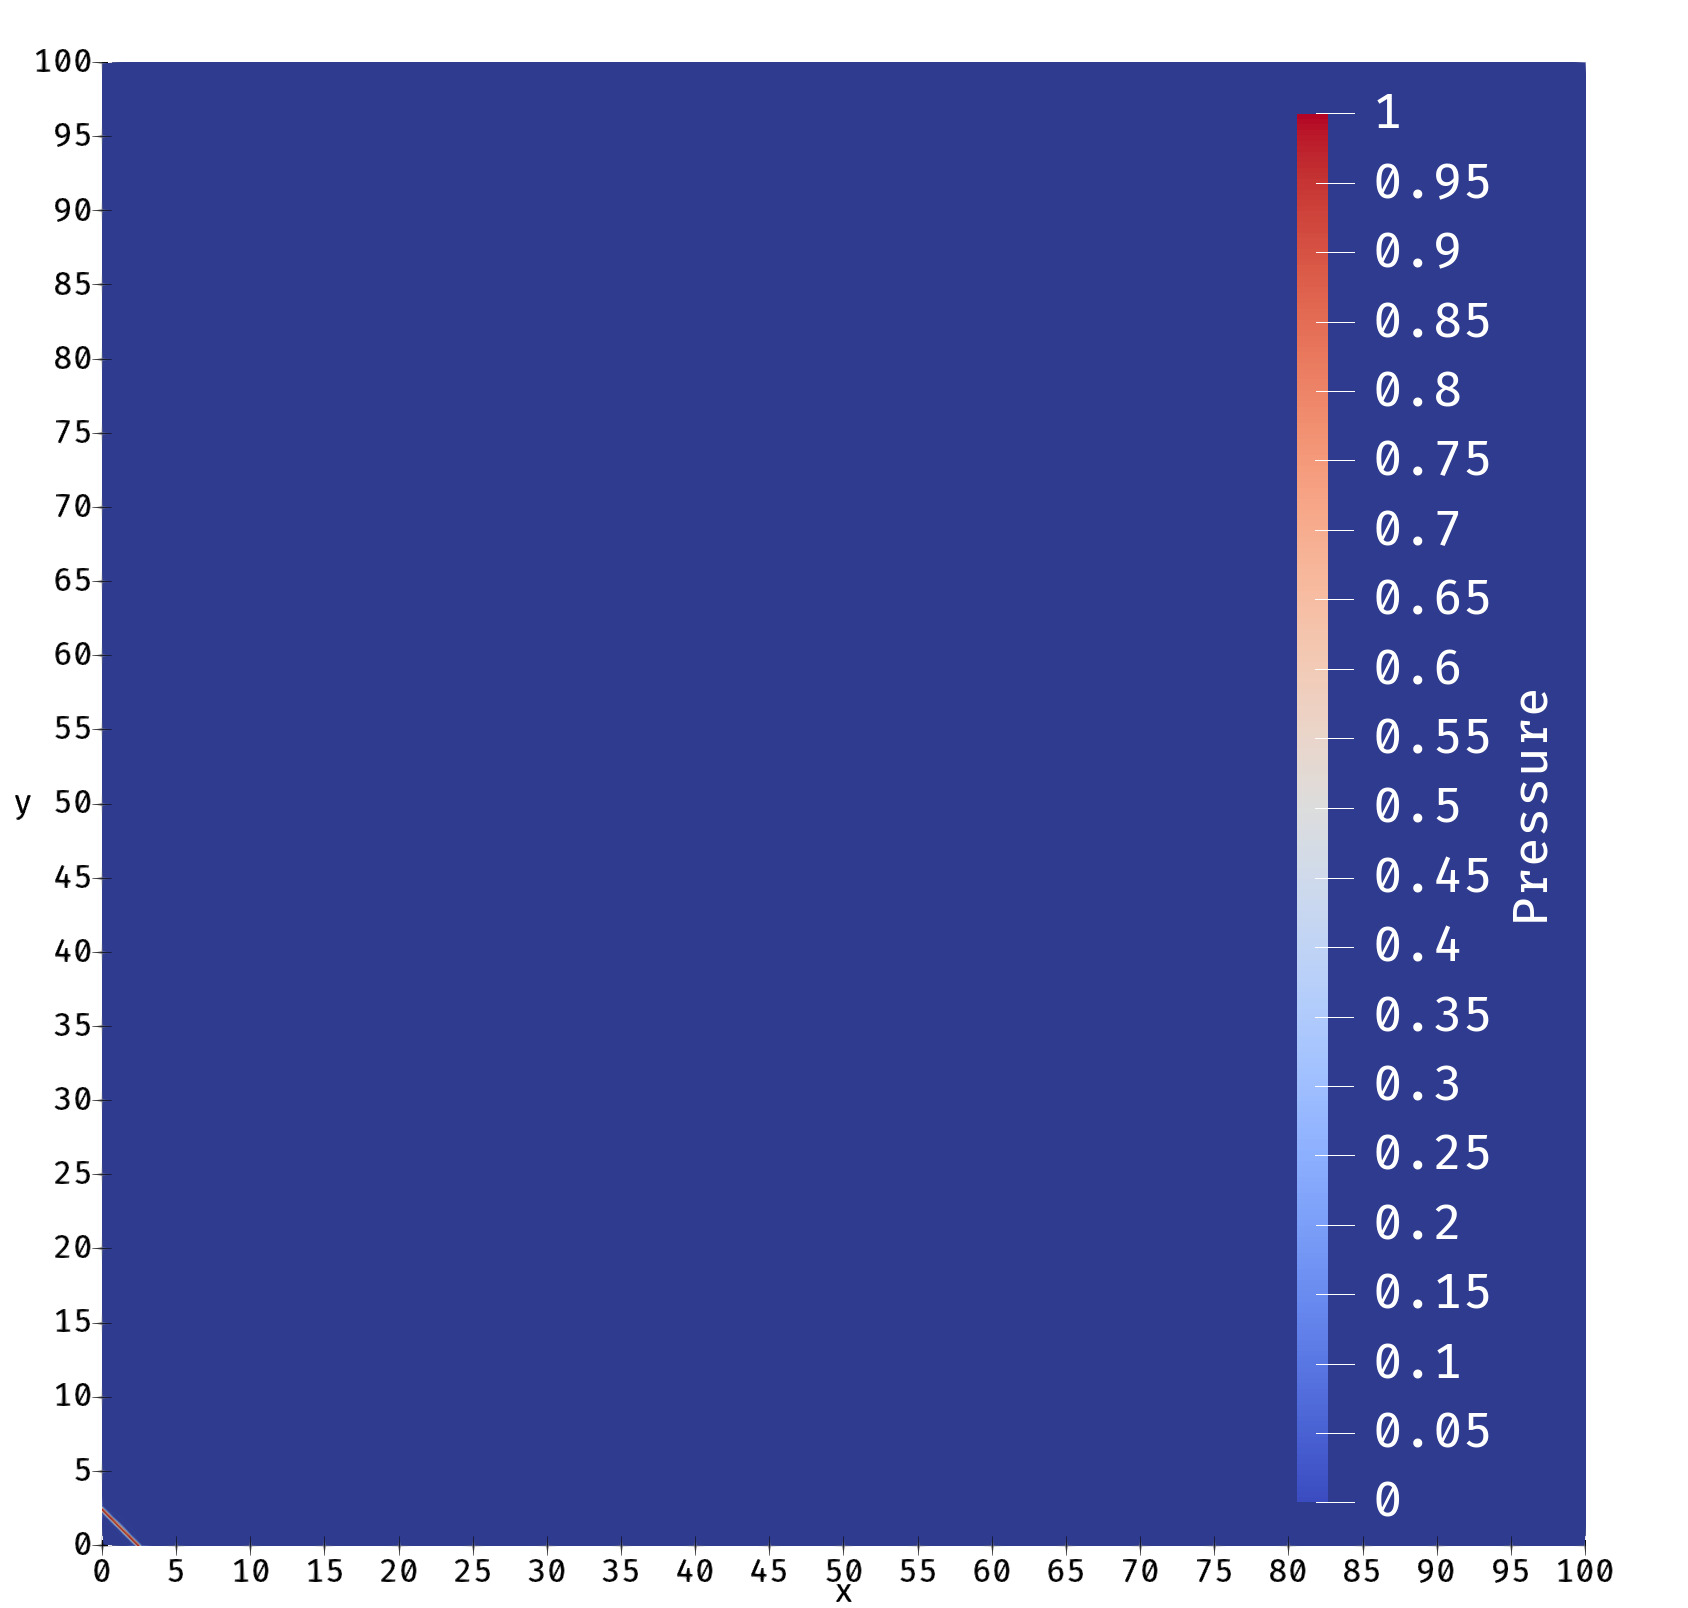
\includegraphics[width=0.5\textwidth]{Chapter_results/media/problem_medium_far}\label{fig:load_imbalance_case_medium_p_far}}
    \hfill
    \subfloat[Detail]
    {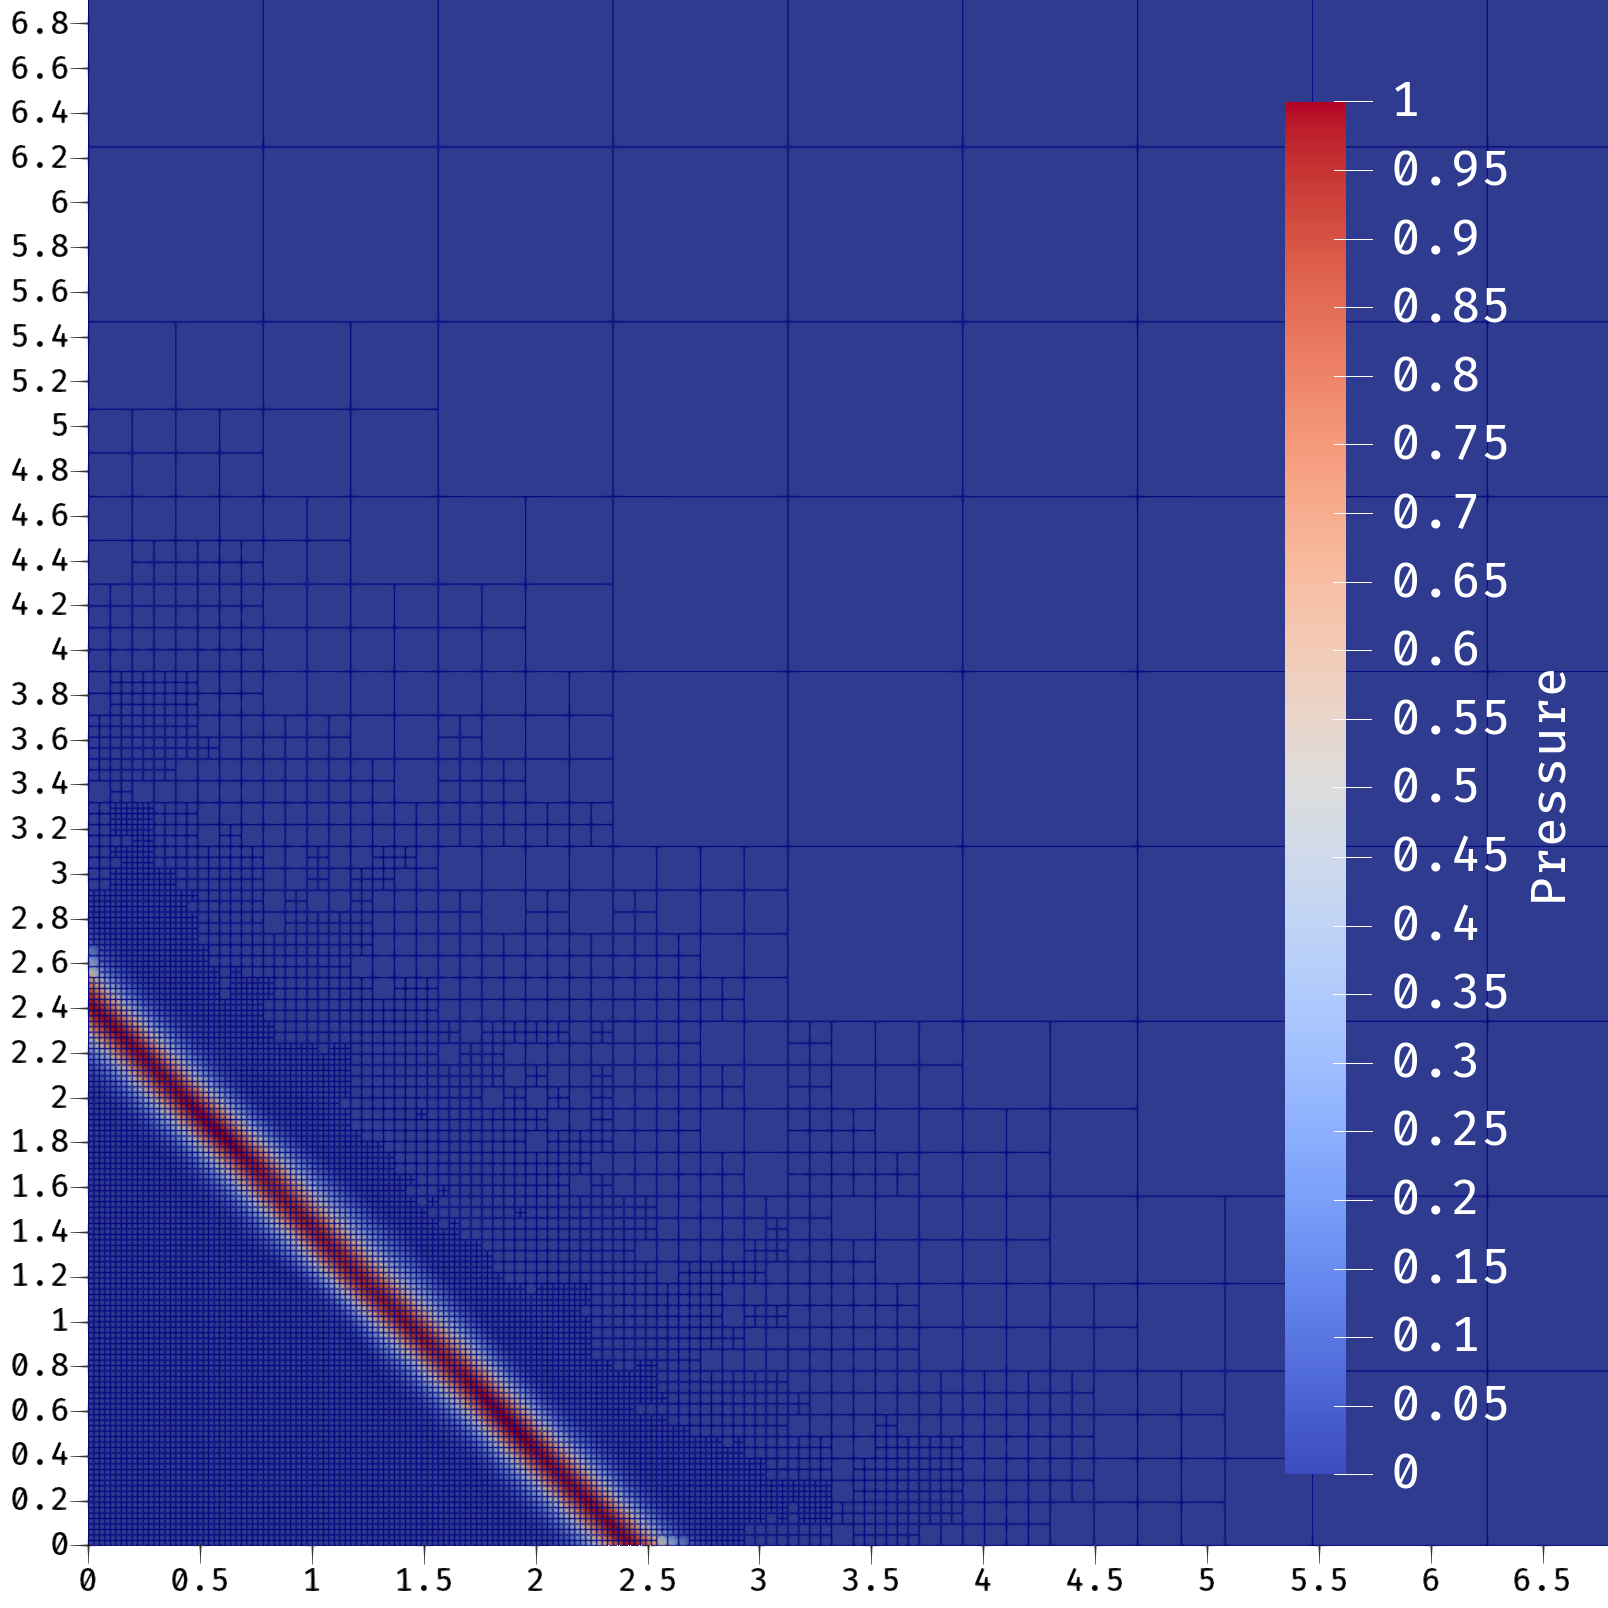
\includegraphics[width=0.48\textwidth]{Chapter_results/media/problem_medium_near}\label{fig:load_imbalance_case_medium_p_near}}
    \caption{Medium load imbalance (\(S = 5\)) test case pressure: A wave passes through a very big domain. \(K_{initial} = 16384\), \(K_{final} = 26734\) (a) Complete domain (b) Area of interest}\label{fig:load_imbalance_case_medium_p}
\end{figure}

\begin{figure}[H]
    \centering
    \subfloat[Full domain]
    {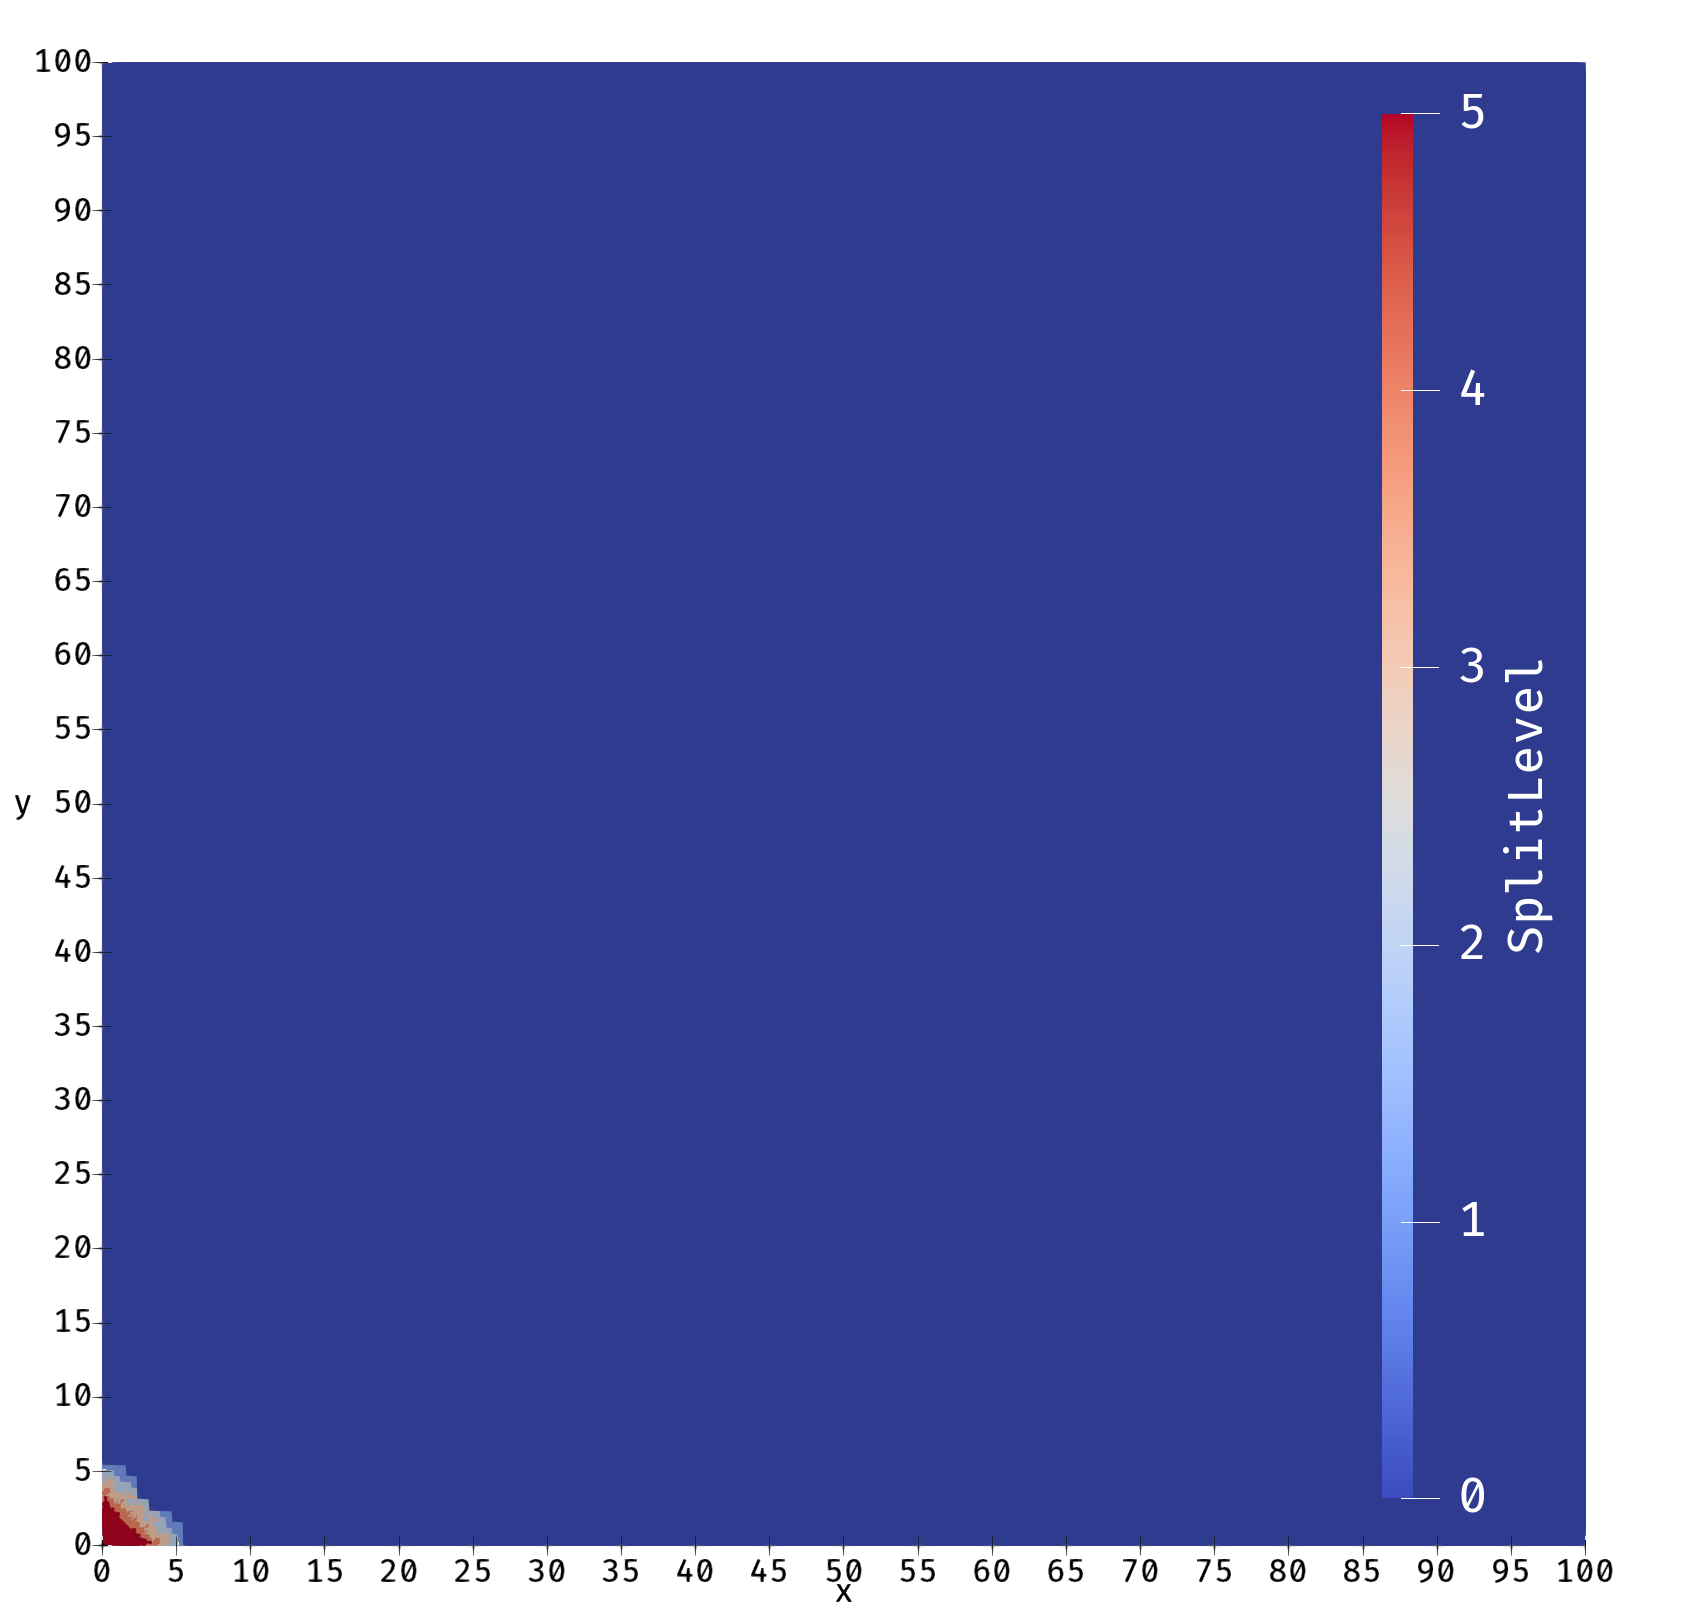
\includegraphics[width=0.5\textwidth]{Chapter_results/media/split_level_medium_far}\label{fig:load_imbalance_case_s_far}}
    \hfill
    \subfloat[Detail]
    {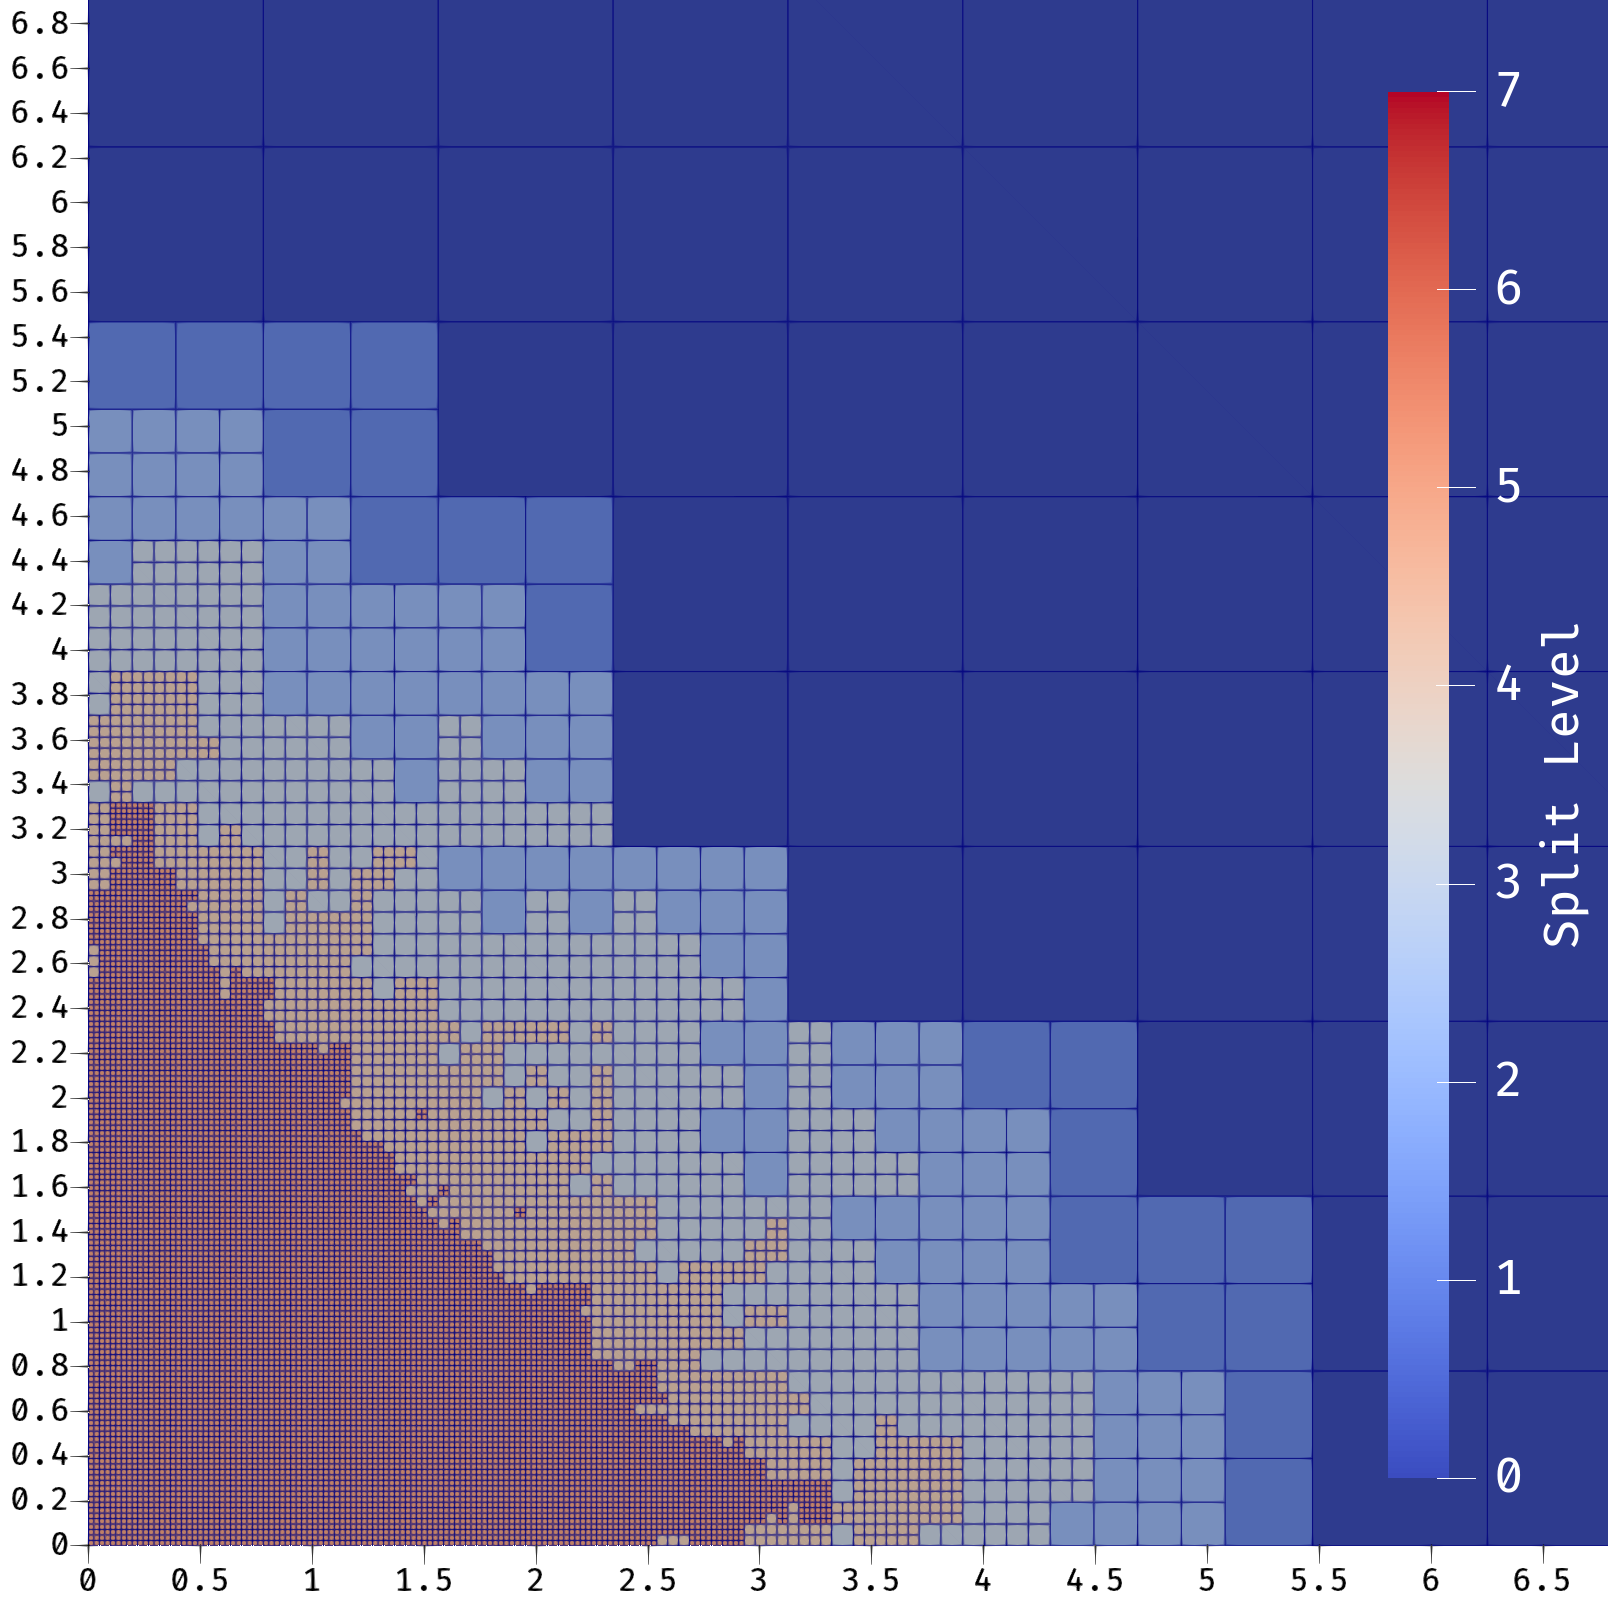
\includegraphics[width=0.48\textwidth]{Chapter_results/media/split_level_medium_near}\label{fig:load_imbalance_case_s_near}}
    \caption{Medium load imbalance (\(S = 5\)) test case split level: Split level, indicating how many times the elements have split, only the bottom left refines. \(K_{initial} = 16384\), \(K_{final} = 26734\) (a) Complete domain (b) Area of interest}\label{fig:load_imbalance_case_medium_s}
\end{figure}

\begin{figure}[H]
    \centering
    \subfloat[Full domain]
    {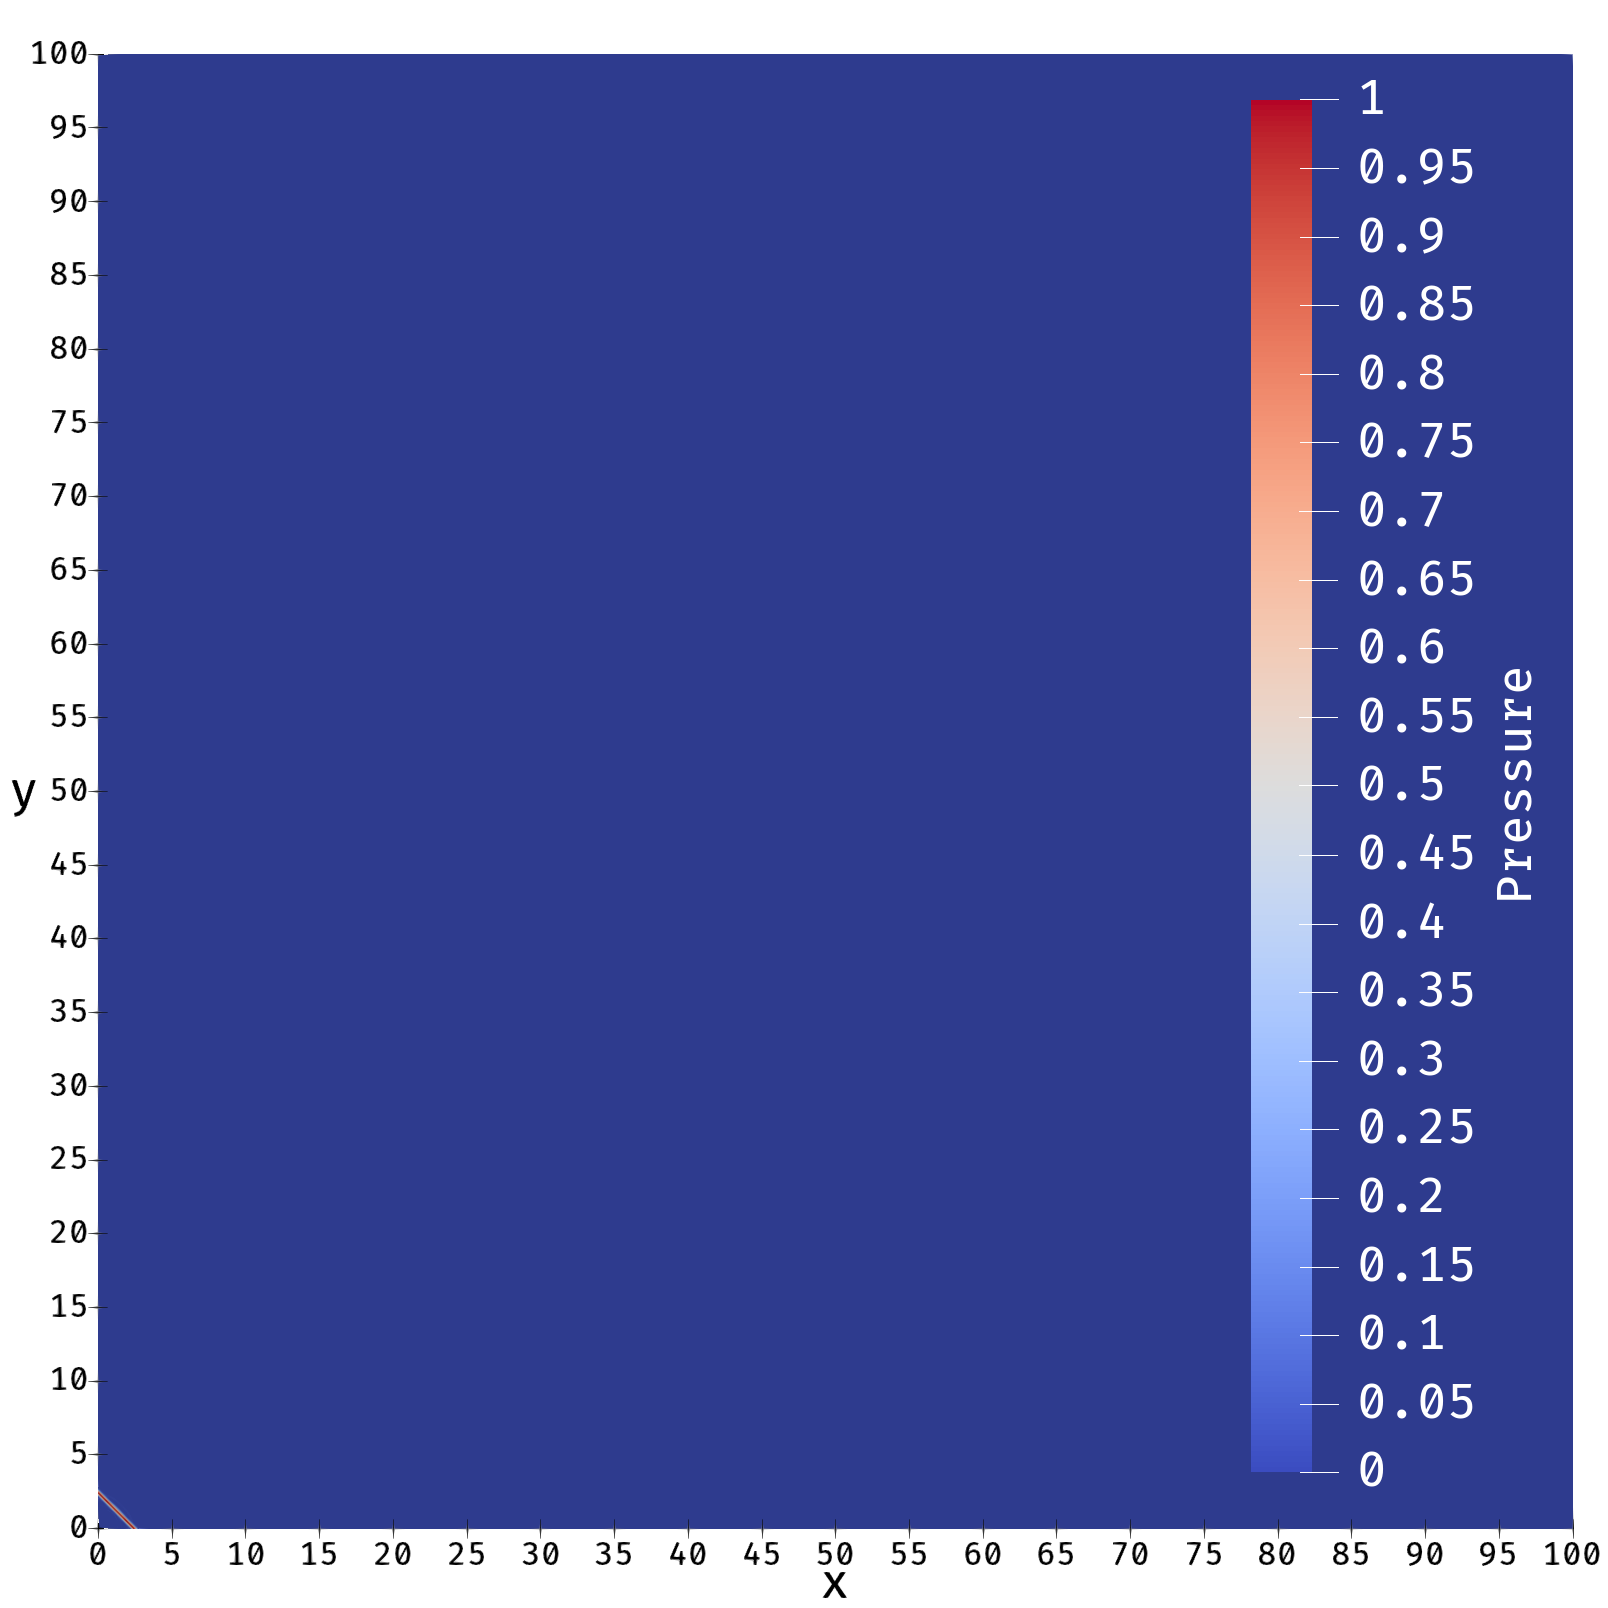
\includegraphics[width=0.5\textwidth]{Chapter_results/media/problem_high_far}\label{fig:load_imbalance_case_high_p_far}}
    \hfill
    \subfloat[Detail]
    {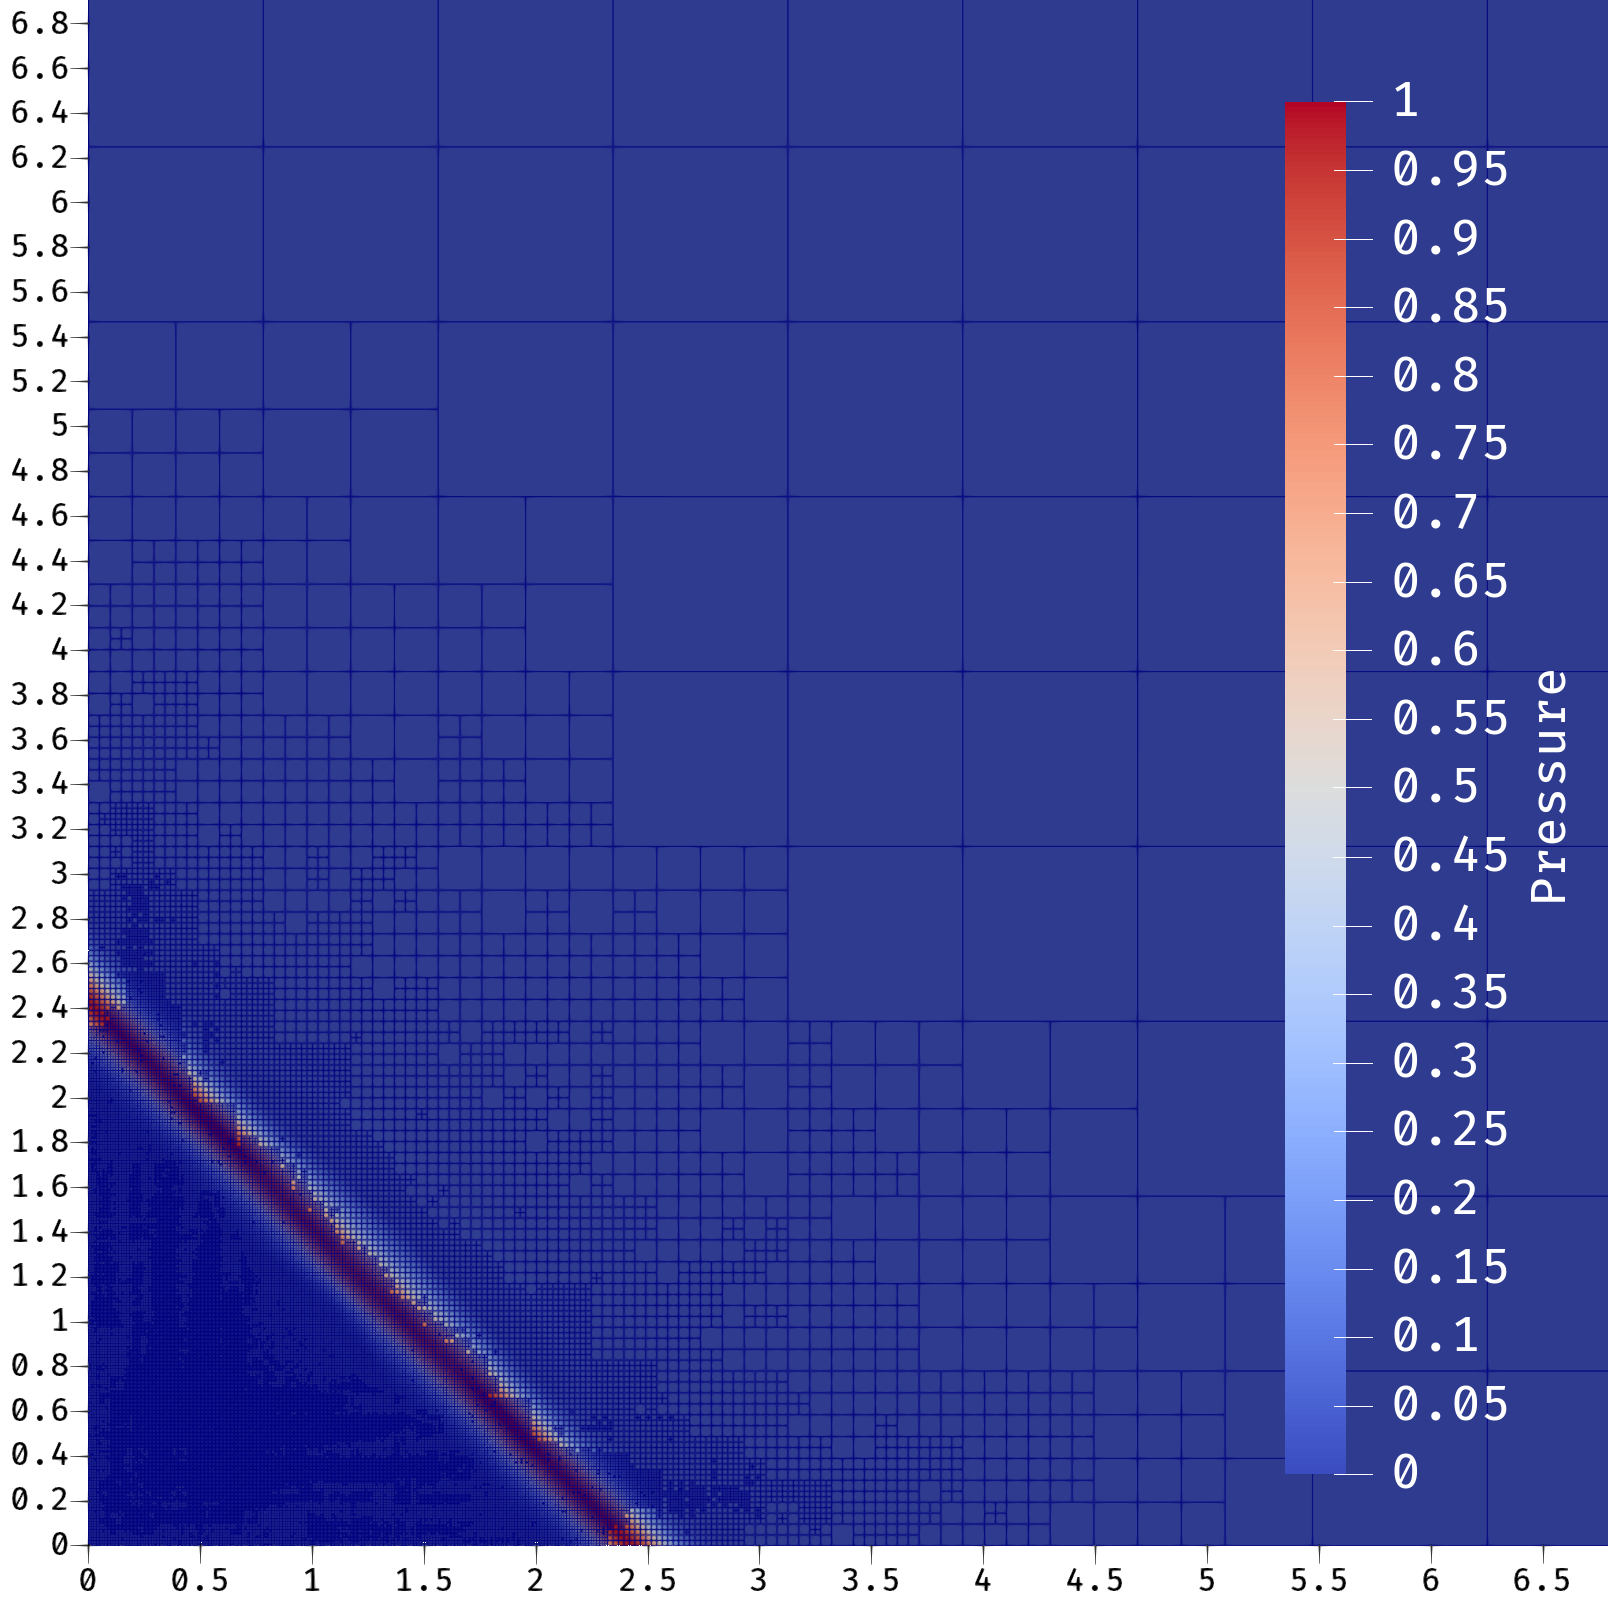
\includegraphics[width=0.48\textwidth]{Chapter_results/media/problem_high_near}\label{fig:load_imbalance_case_high_p_near}}
    \caption{High load imbalance (\(S = 7\)) test case pressure: A wave passes through a very big domain. \(K_{initial} = 16384\), \(K_{final} = 54837\) (a) Complete domain (b) Area of interest}\label{fig:load_imbalance_case_high_p}
\end{figure}

\begin{figure}[H]
    \centering
    \subfloat[Full domain]
    {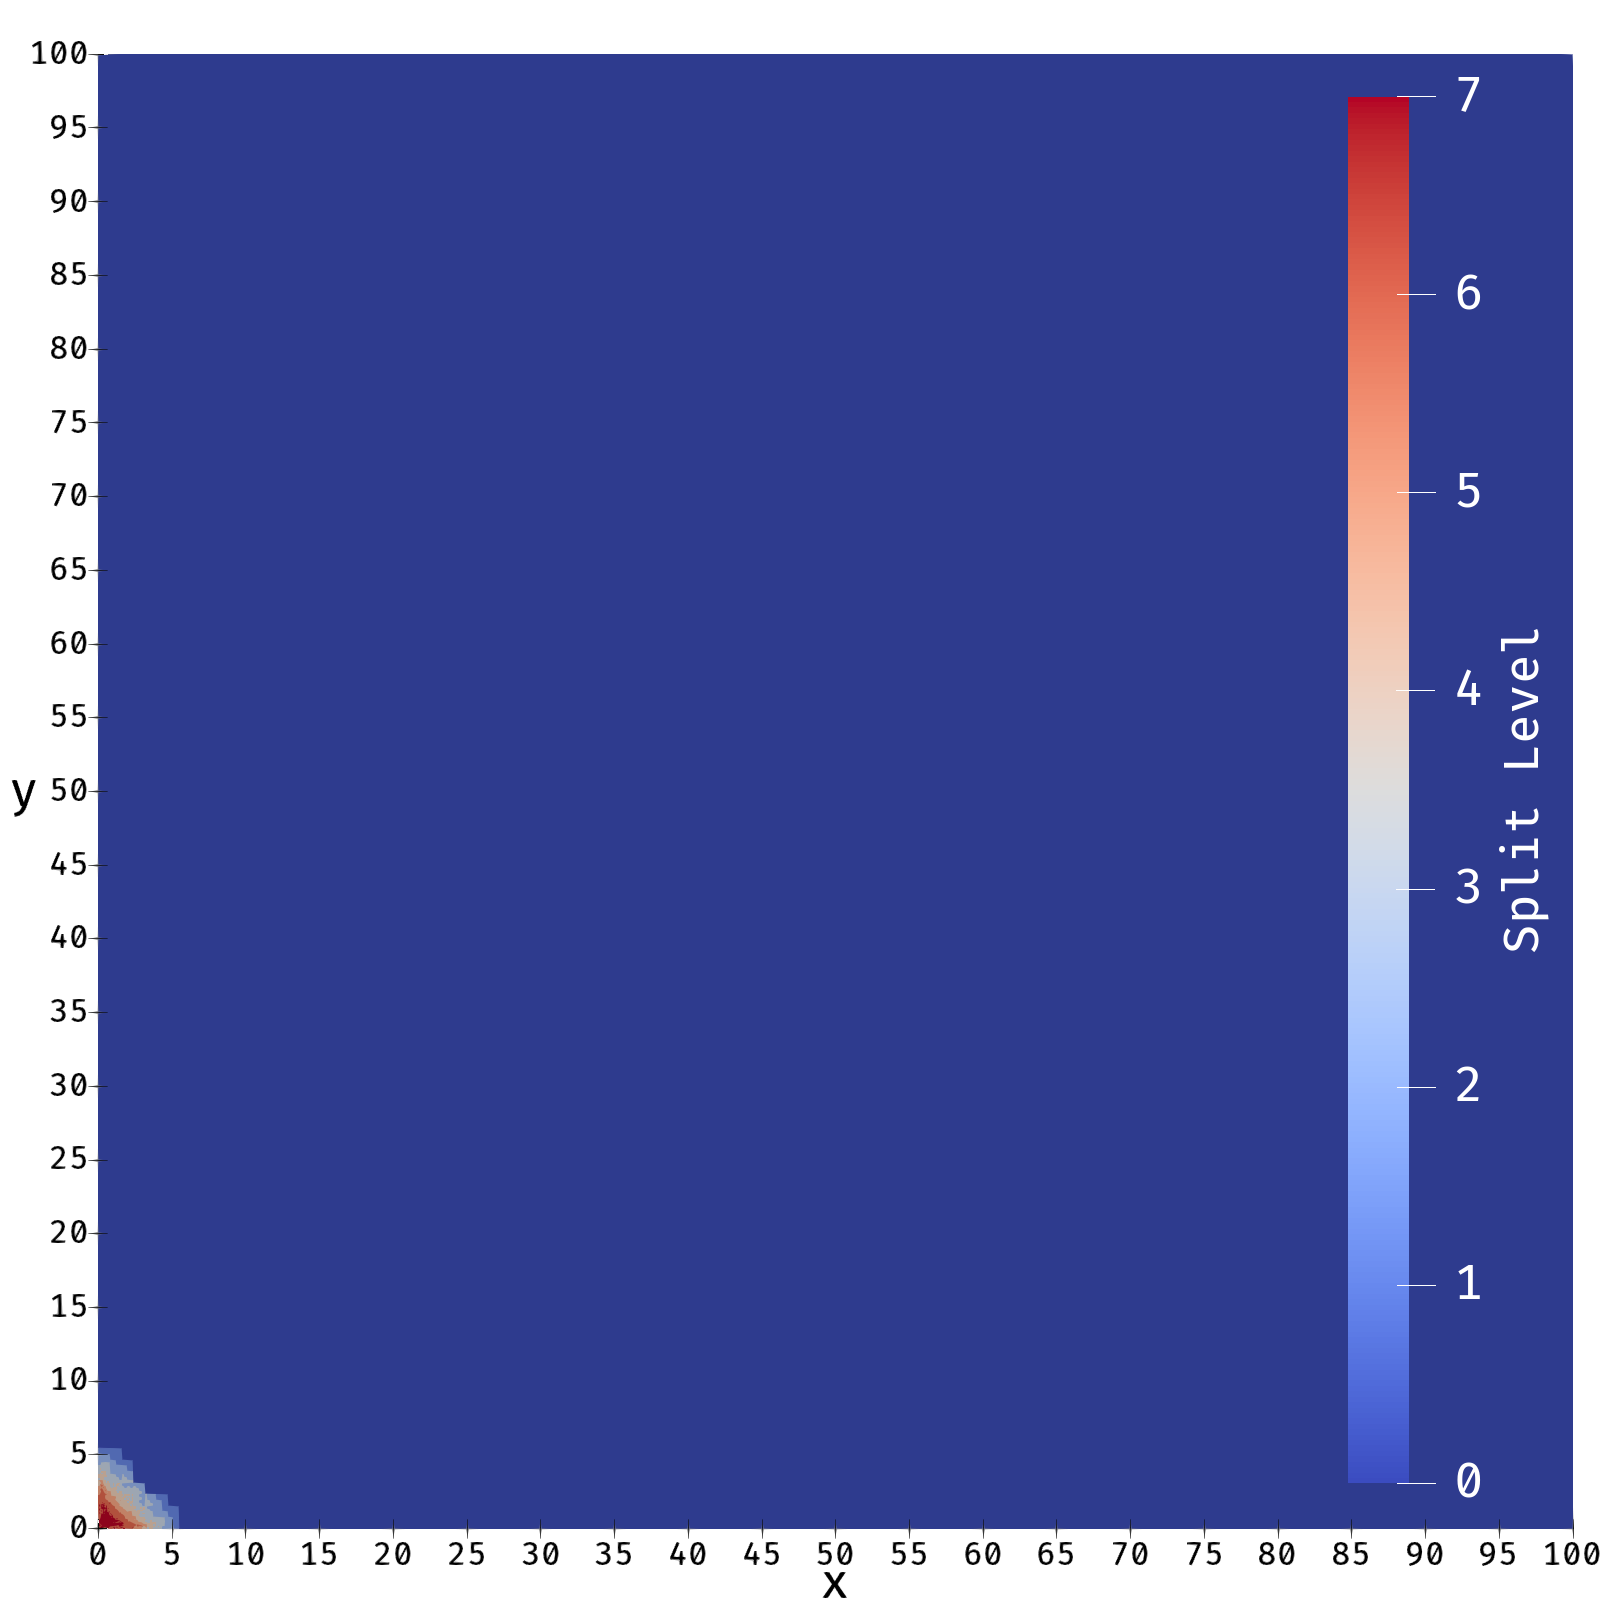
\includegraphics[width=0.5\textwidth]{Chapter_results/media/split_level_high_far}\label{fig:load_imbalance_case_high_s_far}}
    \hfill
    \subfloat[Detail]
    {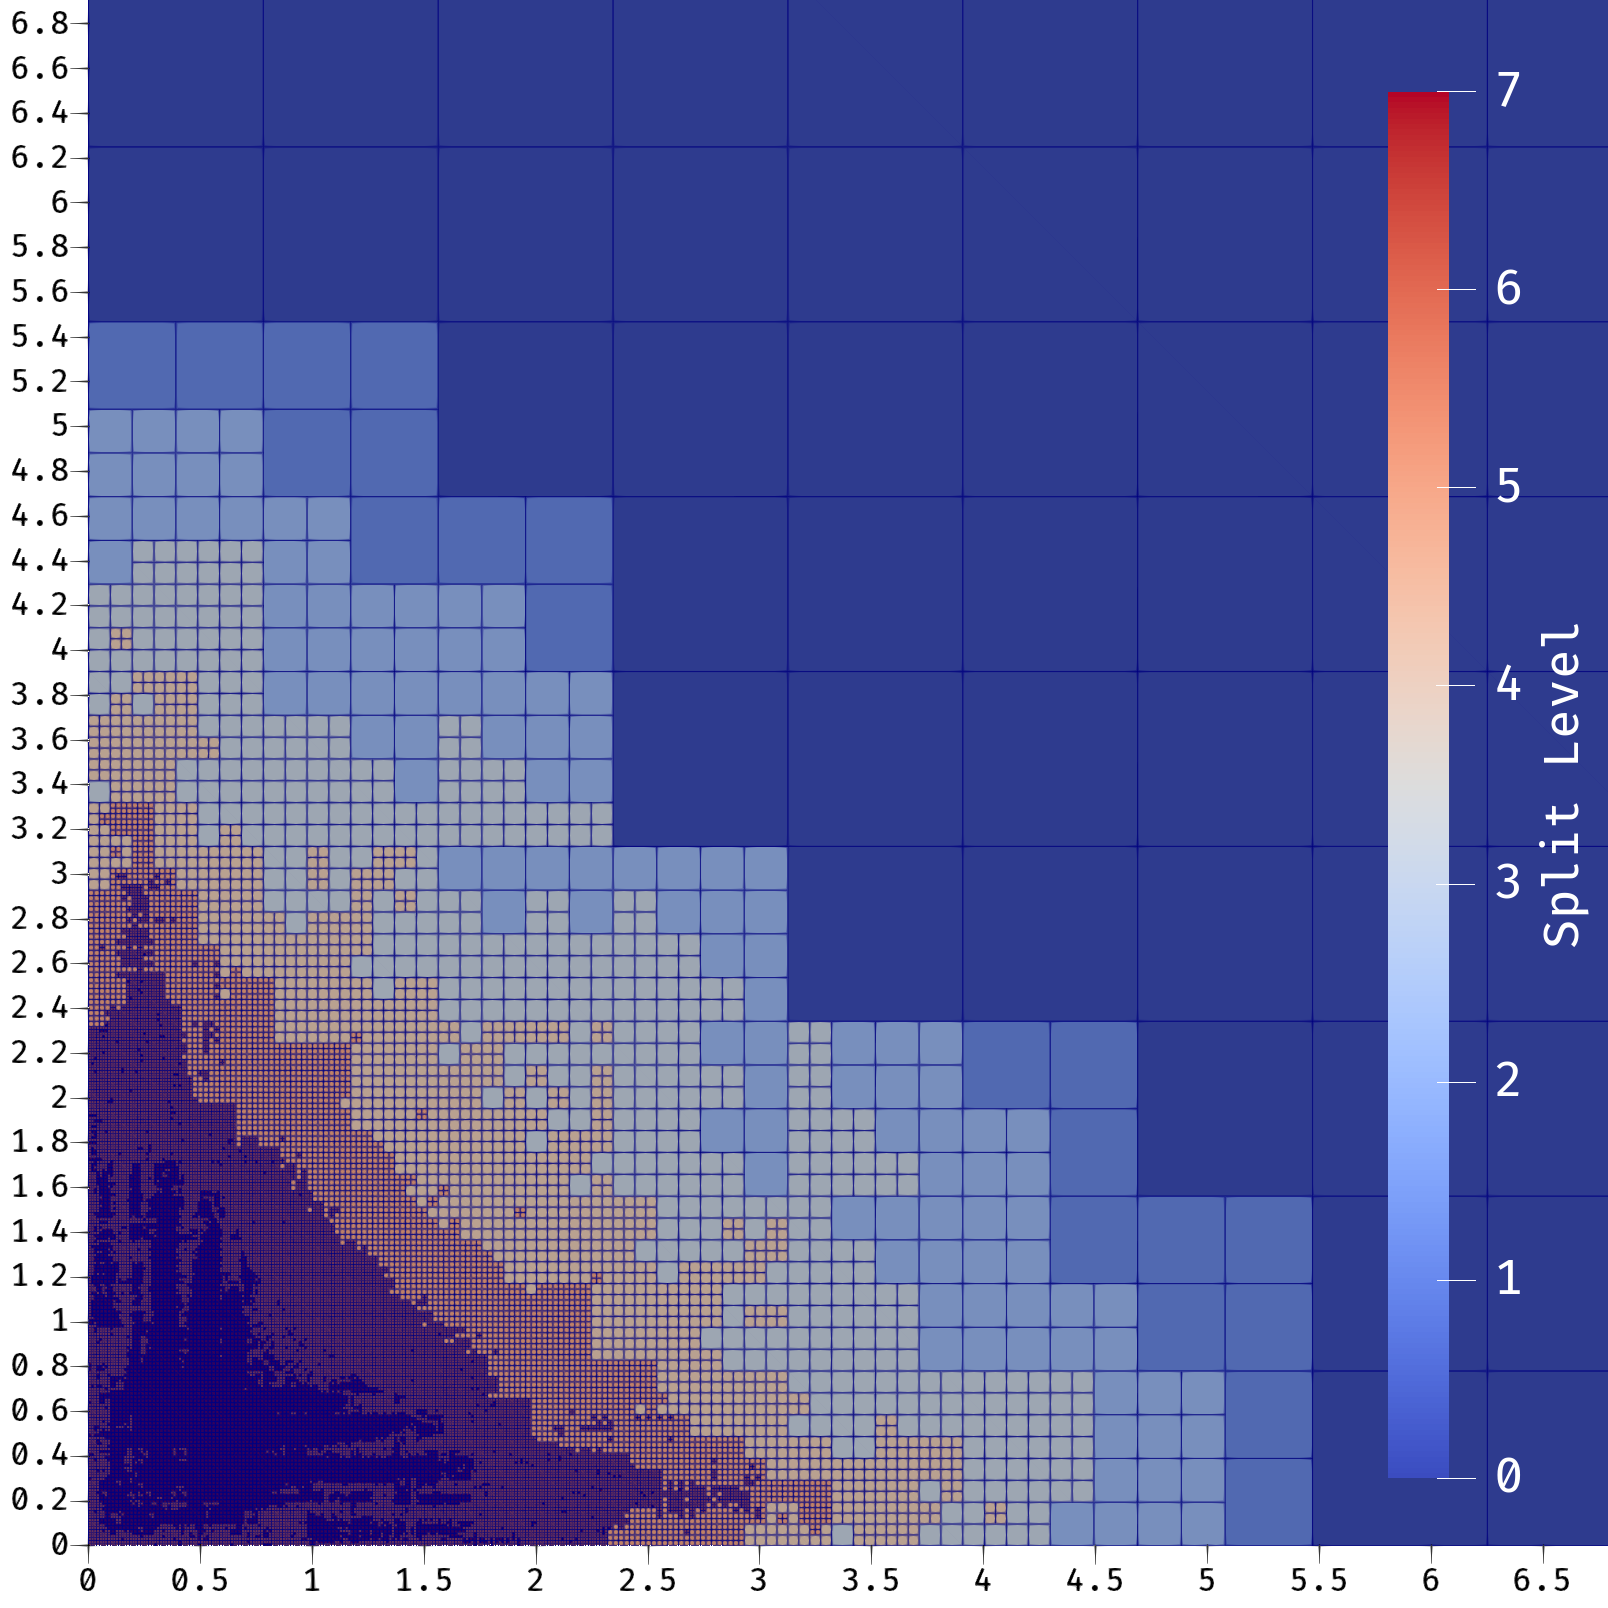
\includegraphics[width=0.48\textwidth]{Chapter_results/media/split_level_high_near}\label{fig:load_imbalance_case_high_s_near}}
    \caption{High load imbalance (\(S = 7\)) test case split level: Split level, indicating how many times the elements have split, only the bottom left refines. \(K_{initial} = 16384\), \(K_{final} = 54837\) (a) Complete domain (b) Area of interest}\label{fig:load_imbalance_case_high_s}
\end{figure}

Table~\ref{table:load_imbalance} describes the load imbalance of the three cases. \(S\) is the
maximum number of times an element can split, \(K\) is the number of elements in the mesh, \(K_p\)
is the number of elements in process \(p\), \(w_{ideal}\) is the number of elements in a process if
evenly distributed, and \(L\) is the load imbalance as described in
Equation~\ref{equ:load_imbalance}.

\begin{table}[H]
    \centering
    \begin{tabular}{ c c c c c c c }
        Case & S & K & Max \(K_p\) & \(w_{ideal}\) & \(L\) \\
        \midrule
        Low & \(3\) & \(17752\) & \(2392\) & \(1110\) & \(2.16\) \\
        Medium & \(5\) & \(26734\) & \(11374\) & \(1671\) & \(6.81\) \\
        High & \(7\) & \(62490\) & \(47130\) & \(3906\) & \(12.07\) \\
    \end{tabular}
    \caption{Load imbalance cases.}\label{table:load_imbalance}
\end{table}

We compare two approaches to choose when to load balance the mesh, as described in
Section~\ref{section:load_balancing:criteria}. We compare the three cases above with and without
load balancing.

\subsection{Load balancing interval}\label{subsection:results:load_balancing_performance:interval}

We start by varying the load balancing interval for the three cases in
Figures~\ref{fig:load_balancing_efficiency_interval_s3},~\ref{fig:load_balancing_efficiency_interval_s5}
and~\ref{fig:load_balancing_efficiency_interval_s7}. Since we refine the mesh every 20 time steps, a
load balancing interval of 20 is equivalent to load balancing the mesh every time we refine it, up
to every 50 times we refine for a load balancing interval of 1000. The dashed line represents the
performance without load balancing.

\begin{figure}[H]
    \begin{adjustwidth}{-0.5in}{-0.5in}
    \centering
    \subfloat[Low load imbalance]
    {\includesvg[width=0.39\textwidth]{Chapter_results/media/load_balancing_interval_N4_K16384_A20_P16_S3}\label{fig:load_balancing_efficiency_interval_s3}}
    \hfill
    \subfloat[Medium load imbalance]
    {\includesvg[width=0.39\textwidth]{Chapter_results/media/load_balancing_interval_N4_K16384_A20_P16_S5}\label{fig:load_balancing_efficiency_interval_s5}}
    \hfill
    \subfloat[High load imbalance]
    {\includesvg[width=0.39\textwidth]{Chapter_results/media/load_balancing_interval_N4_K16384_A20_P16_S7}\label{fig:load_balancing_efficiency_interval_s7}}
    \end{adjustwidth}
    \caption{Load balancing performance interval test: Simulation time with refinement and load balancing while increasing load balancing interval. \(N_{initial} = 4\), \(K_{initial} = 16384\), refinement interval = 20, \(P = 16\) (a) \(S = 3\) (b) \(S = 5\) (c) \(S = 7\)}\label{fig:load_balancing_efficiency_interval}
\end{figure}

From Figure~\ref{fig:load_balancing_efficiency_interval}, we see that load balancing diminishes the
computation time of all three problems. The low load imbalance case needs a higher load balancing
interval to offset the cost of the load balancing algorithm. In the other cases, the load imbalance
is great enough that the cases with load balancing are always faster. It takes a certain load
balancing interval to obtain the best performance, and that interval changes with the case. Next, we
will study an alternative algorithm to improve on those two points.

\subsection{Load balancing threshold}\label{subsection:results:load_balancing_performance:threshold}

We now use an allowable load imbalance threshold to choose when to perform load balancing, as
described in Section~\ref{section:load_balancing:criteria}. This means we assess the load imbalance
\(L\) of the mesh after each refinement step, and we only perform load balancing if it is above a
certain threshold. We start with a threshold of \(1\), equivalent to load balancing after every
refinement step, to \(2\), equivalent to load balancing only if a \acrshort{acr:GPU} has two or more
times the workload it would have if the mesh was perfectly balanced. The same three load imbalance
cases from Section~\ref{section:results:load_balancing_performance} are shown in
Figure~\ref{fig:load_balancing_efficiency_threshold}.

\begin{figure}[H]
    \begin{adjustwidth}{-0.5in}{-0.5in}
    \centering
    \subfloat[Low load imbalance]
    {\includesvg[width=0.39\textwidth]{Chapter_results/media/load_balancing_threshold_N4_K16384_A20_L20_P16_S3}\label{fig:load_balancing_efficiency_threshold_s3}}
    \hfill
    \subfloat[Medium load imbalance]
    {\includesvg[width=0.39\textwidth]{Chapter_results/media/load_balancing_threshold_N4_K16384_A20_L20_P16_S5}\label{fig:load_balancing_efficiency_threshold_s5}}
    \hfill
    \subfloat[High load imbalance]
    {\includesvg[width=0.39\textwidth]{Chapter_results/media/load_balancing_threshold_N4_K16384_A20_L20_P16_S7}\label{fig:load_balancing_efficiency_threshold_s7}}
    \end{adjustwidth}
    \caption{Load balancing performance threshold test: Simulation time with refinement and load balancing while increasing load balancing threshold. \(N_{initial} = 4\), \(K_{initial} = 16384\), refinement interval = 20, load balancing interval = 20, \(P = 16\) (a) \(S = 3\) (b) \(S = 5\) (c) \(S = 7\)}\label{fig:load_balancing_efficiency_threshold}    
\end{figure}

From Figure~\ref{fig:load_balancing_efficiency_threshold}, we observe that using a load imbalance
threshold to control when we load balance is a much better solution than simply increasing the
interval at which we perform load balancing. The performance improves quickly when increasing the
threshold, and the threshold values that work well do not seem to change with the problem. A load
imbalance threshold of around \(1.1\) seems to give good performance in all cases, and would not
need to be adapted to different cases.

\subsection{Overall load balancing performance}\label{subsection:results:load_balancing_performance:overall}

From the results of Subsections~\ref{subsection:results:load_balancing_performance:interval}
and~\ref{subsection:results:load_balancing_performance:threshold}, we observe that load balancing at
every occasion incurs a significant performance penality, sometimes performing worse than the non
load-balanced case in the low load imbalance case, in
Figures~\ref{fig:load_balancing_efficiency_interval_s3}
and~\ref{fig:load_balancing_efficiency_threshold_s3}. The two other cases also show worse
performance with a low load balancing interval or load imbalance threshold. This is because the
dynamic load balancing process is expensive, especially since we are using \acrshortpl{acr:GPU},
because of the numerous data transfers and memory allocations performed. We must choose judiciously
our load balancing strategy. 

The performance increases as we space out load balancing, either by increasing the load balancing
interval, or by increasing the load imbalance threshold, up to a point. Past that point, an interval
of \(500\) or a threshold of \(1.5\) in this case, the performance goes down due to the mesh being
more imbalanced for longer periods of time.

The load imbalance threshold strategy from
Subsection~\ref{subsection:results:load_balancing_performance:threshold} gives better results, the
performance improves quickly when increasing the threshold and stays high longer than the load
balancing interval strategy from
Subsection~\ref{subsection:results:load_balancing_performance:interval}. The load balancing interval
is also case dependent, and must be adjusted according to the scale of the problem and how often it
is refined. 

For these reasons we choose the load imbalance threshold strategy with a load imbalance threshold of
\(1.1\) to assess the overall dynamic load balancing performance in
Figure~\ref{fig:load_balancing_efficiency}. It shows the speedup we get from load balancing the
three problems. The \(x\) axis represents the equivalent load imbalance \(L\) of the problems if
they were not load balanced.

\begin{figure}[H]
    \centering
    \includesvg[width=0.6\textwidth]{Chapter_results/media/load_balancing_threshold_N4_K16384_A20_L20_P16_T1.1}
    \caption{Load balancing performance: Simulation time with refinement and load balancing while increasing load imbalance. \(N_{initial} = 4\), \(K_{initial} = 16384\), refinement interval = 20, load balancing interval = 20, \(P = 16\), load balancing threshold = \(1.1\)}\label{fig:load_balancing_efficiency}
\end{figure}

Figure~\ref{fig:load_balancing_efficiency} shows that dynamic load balancing performs well, and is
able to regain performance lost to load imbalance. In the high load imbalance case, with a load
imbalance of \(L = 12.07\), dynamic load balancing can improve performance by \(4.1 \times \). It
scales well with load imbalance, meaning it gives good results no matter the level of imbalance of
the problem. The gains are especially crucial for high imbalance levels, where the load imbalance
can degrade performance by an order of magnitude. In these cases, dynamic load balancing can regain
most of the lost performance.

\subsection{Polynomial order influence}\label{subsection:results:load_balancing_performance:polynomial_order}

Figure~\ref{fig:N_influence} shows a comparison of the iteration time as a function of the
polynomial order \(N\) of a uniformly refined mesh, both on the \acrshort{acr:CPU} and
\acrshort{acr:GPU}. This shows how computing time scales on the two types of processors with
increasing \(N\), and could guide how elements should be weighted individually when performing load
balancing, instead of being all weighted equally as they are in this work. The test case was
computed using the Narval supercomputer, using a grid with \(64\) elements in each of the the \(x\)
and \(y\) directions. The initial polynomial order of the mesh is indicated on the \(y\) axis, and
the problem is advanced by \(1000\) iterations in all cases. \Acrshort{acr:AMR} is performed every
\(100\) iterations, but there are enough elements that the mesh never refines, it only estimates the
error. The \acrshort{acr:CPU} case is computed on a single \acrshort{acr:CPU} core, and the
\acrshort{acr:GPU} case is computed on a single \acrshort{acr:GPU}.

\begin{figure}[H]
    \centering
    \subfloat[\Acrshort{acr:CPU} and \Acrshort{acr:GPU}]
    {\includesvg[width=0.5\textwidth]{Chapter_results/media/N_cpu_iteration_time}\label{fig:N_cpu_influence}}
    \hfill
    \subfloat[\Acrshort{acr:GPU} detail]
    {\includesvg[width=0.48\textwidth]{Chapter_results/media/N_gpu_iteration_time}\label{fig:N_gpu_influence}}
    \caption{Polynomial order influence: Iteration time with increasing polynomial order \(N\). (a)
        \Acrshort{acr:CPU} and \Acrshort{acr:GPU}. (b) \Acrshort{acr:GPU} detail, emphasising the 
        slope.}\label{fig:N_influence}
\end{figure}

Figure~\ref{fig:N_influence} shows that the relation between iteration time and polynomial order
\(N\) on the \acrshort{acr:GPU} is closer to being linear in this range. This is unexpected, as we
expect the relation between polynomial order and computing time to scale with \({\left( N + 1
\right)}^3\) like on the \acrshort{acr:CPU}, as the number of operations to perform on every time
step scales with \({\left( N + 1 \right)}^3\). This may be explained by the fact that
\acrshortpl{acr:GPU} favour more arithmetically intense computations. As \(N\) increases, there are
more compute operations to perform relative to other operations like scheduling and launching
kernels, which may increase the workload of \acrshortpl{acr:GPU} and increase their performance. An
increase in realisable \acrshort{acr:GPU} performance in GFLOPS has been observed when \(N\)
increases, as for example by Chan et al.~\cite{Chan2016}.

\section{Complex Case}\label{section:results:complex_application}

We now present a more complex case with all modules of the program enabled. Figure~\ref{fig:cloud_p}
shows the pressure distribution at two times. The problem depicts a diagonal wave moving through a
small circular ``cloud'' of higher pressure. The cloud expands and interacts with the wave. The mesh
is initially split into \(16\) elements in each of the \(x\) and \(y\) directions, for a total of
\(K = 256\) elements. The polynomial order of the elements is initially \(N = 4\). The solution is
computed in parallel on \(16\) \acrshortpl{acr:GPU}. The mesh is refined every \(50\) timesteps, and
load balanced with an imbalance threshold of \(L = 1.1\). It is allowed to refine up to \(S = 3\)
and \(N = 16\). Three steps of mesh pre-condition are performed, which is why the \(t = 0 s\) mesh
is already refined in Figures~\ref{fig:cloud_s_t0} and~\ref{fig:cloud_N_t0}.
Figure~\ref{fig:cloud_s} shows the split level \(S\) of the mesh, Figure~\ref{fig:cloud_N} the
polynomial order \(N\) of the mesh, and Figure~\ref{fig:cloud_rank} the rank of the elements. The
rank indicates which of the \(16\) \acrshortpl{acr:GPU} is responsible for which part of the mesh,
and how this changes with time as the mesh is load balanced.

\begin{figure}[H]
    \centering
    \subfloat[\( t = 0 s\)]
    {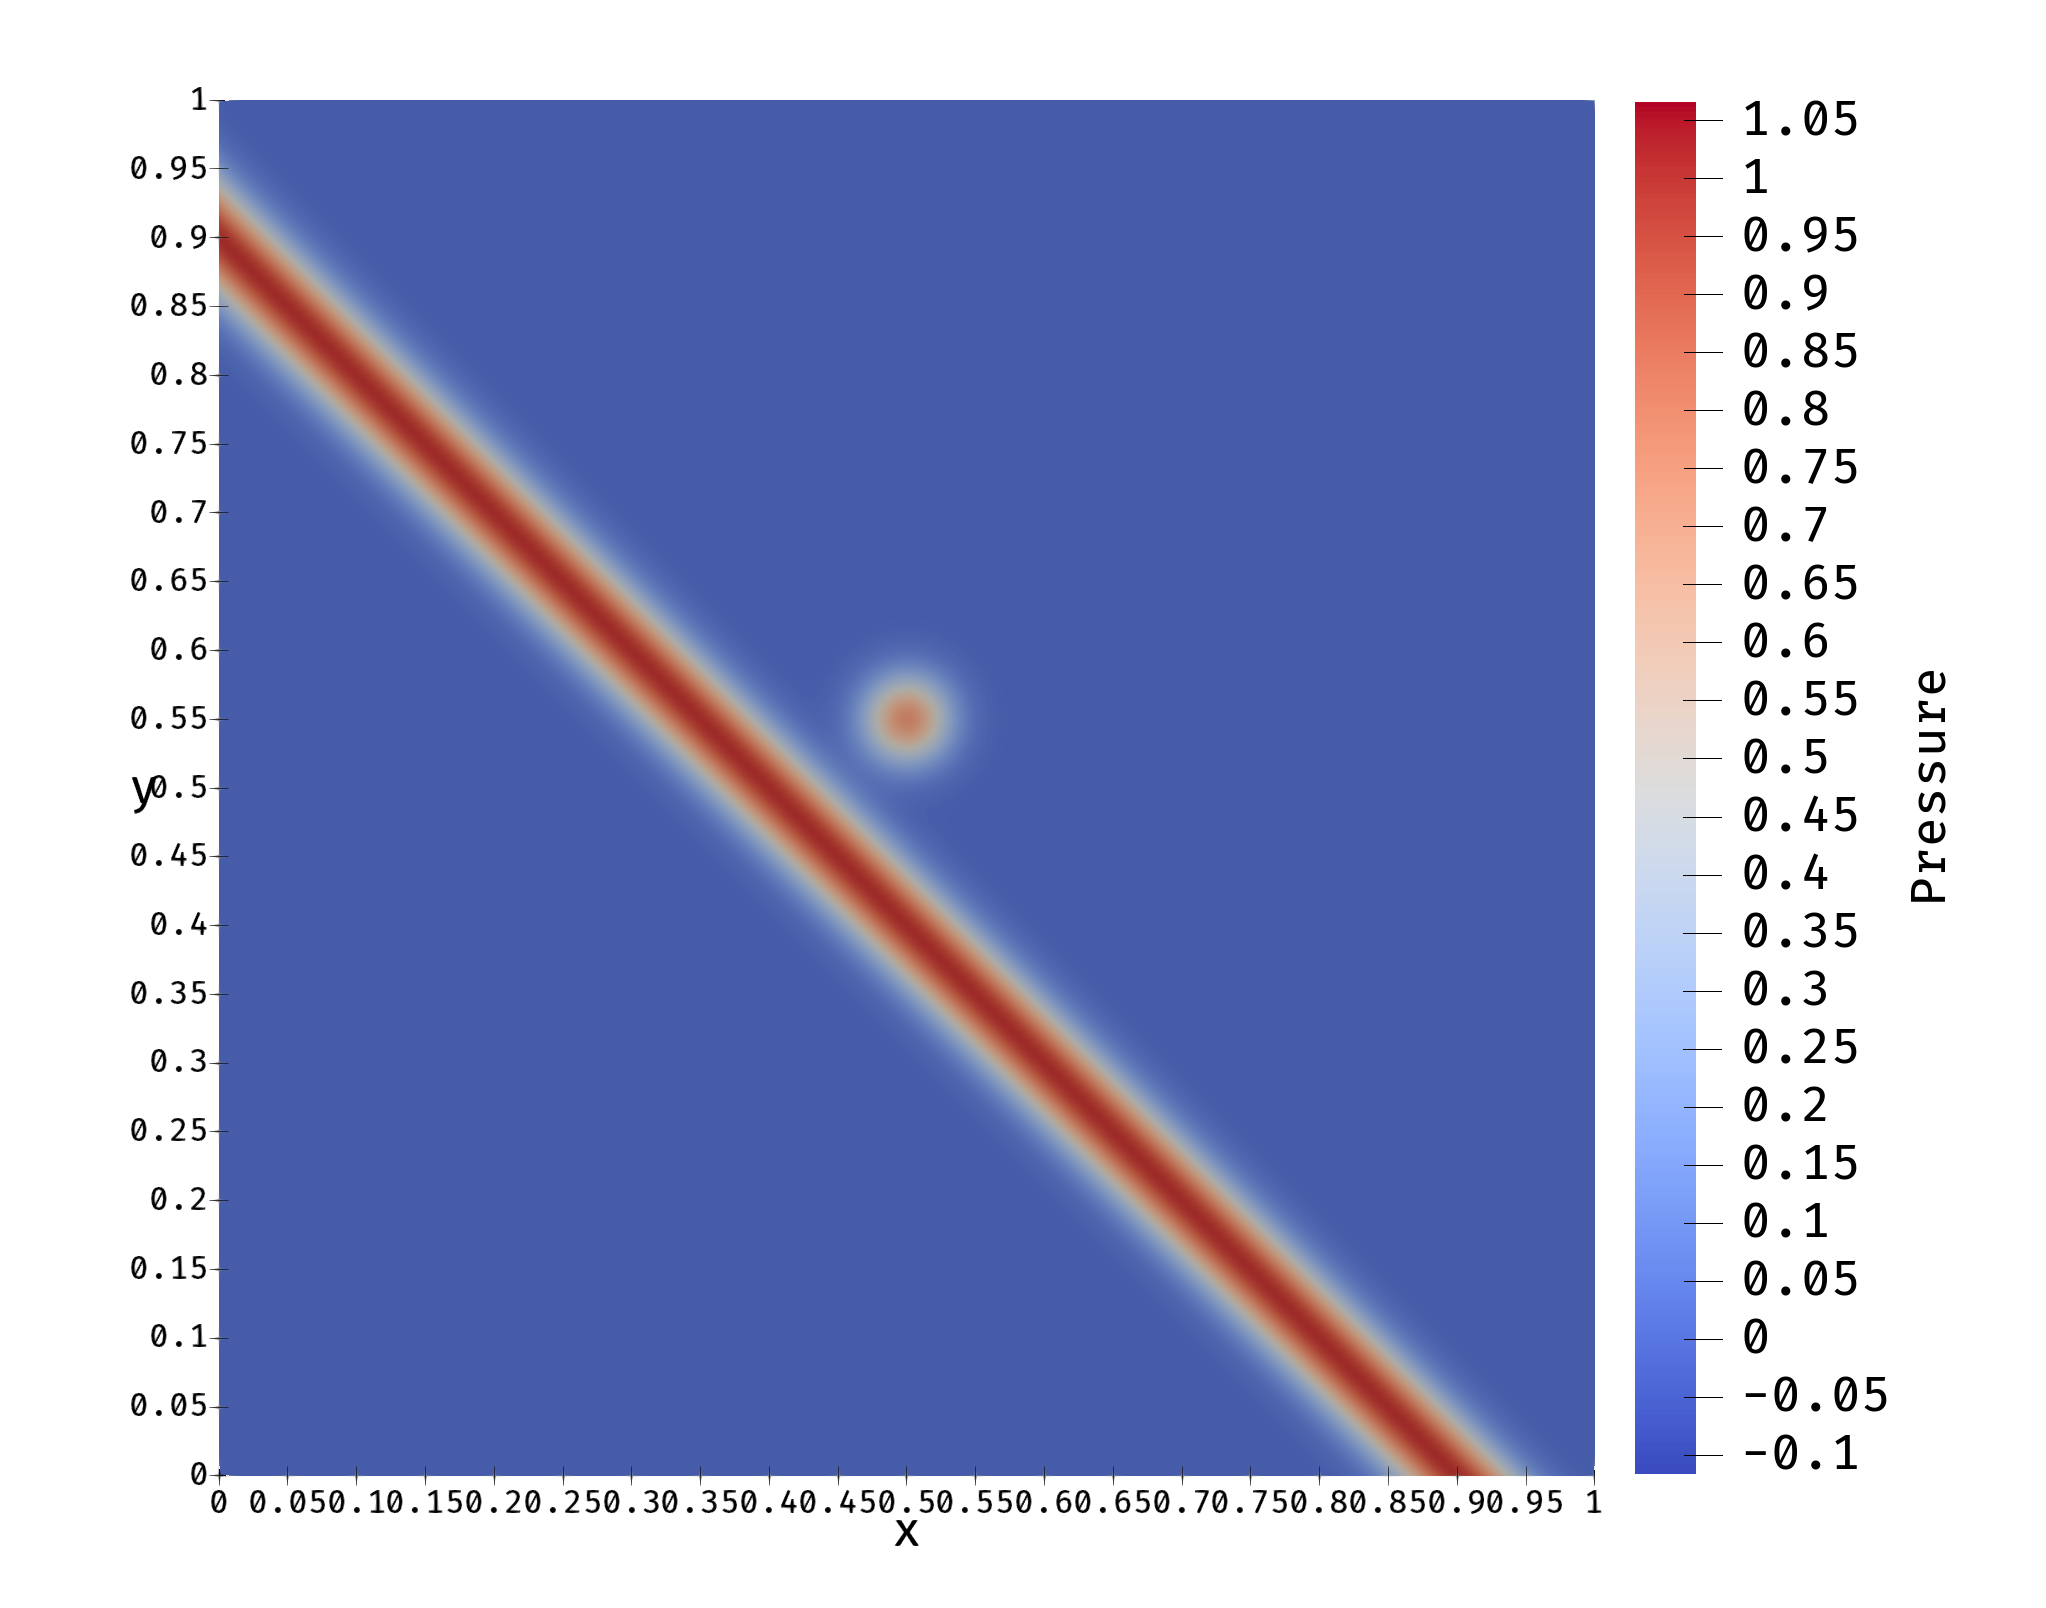
\includegraphics[width=0.48\textwidth]{Chapter_results/media/cloud_t0}\label{fig:cloud_p_t0}}
    \hfill
    \subfloat[\( t = 0.2 s\)]
    {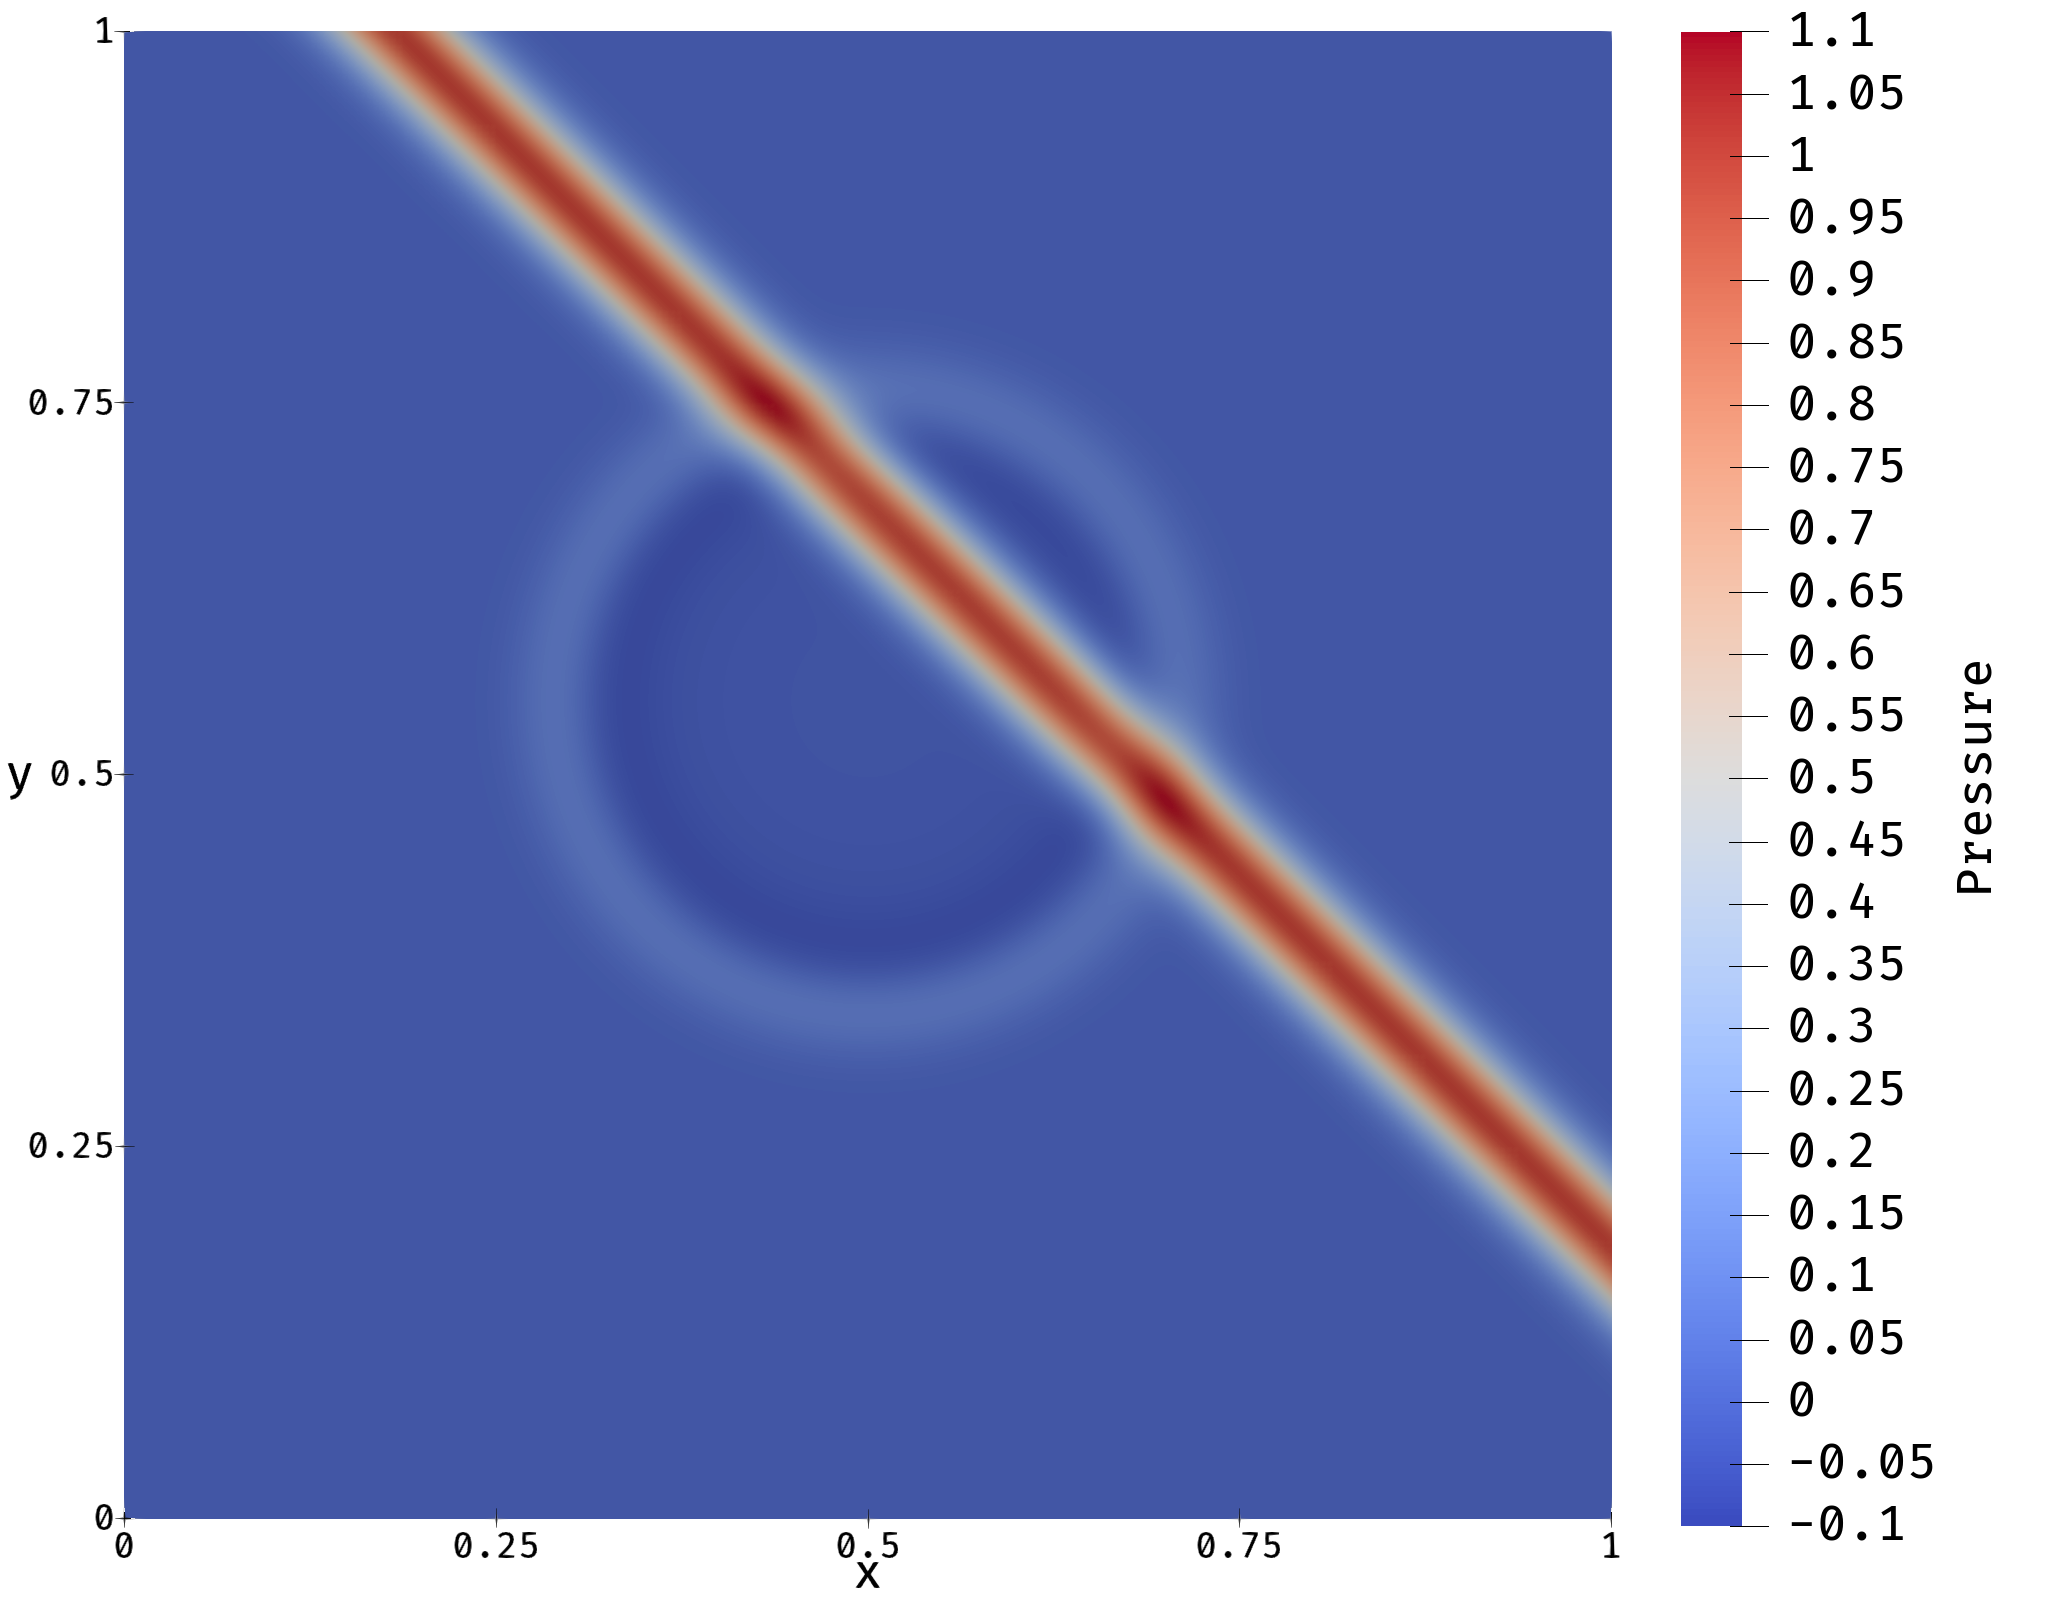
\includegraphics[width=0.48\textwidth]{Chapter_results/media/cloud_t0_2}\label{fig:cloud_p_t0_2}}
    \caption{Complex case: A wave goes through a cloud of high pressure. \(N_{initial} = 4\), \(K_{initial} = 256\), \(S = 3\), \(P = 16\) (a) Initial conditions (b) After the wave and cloud collide}\label{fig:cloud_p}
\end{figure}

\begin{figure}[H]
    \centering
    \subfloat[\( t = 0 s\)]
    {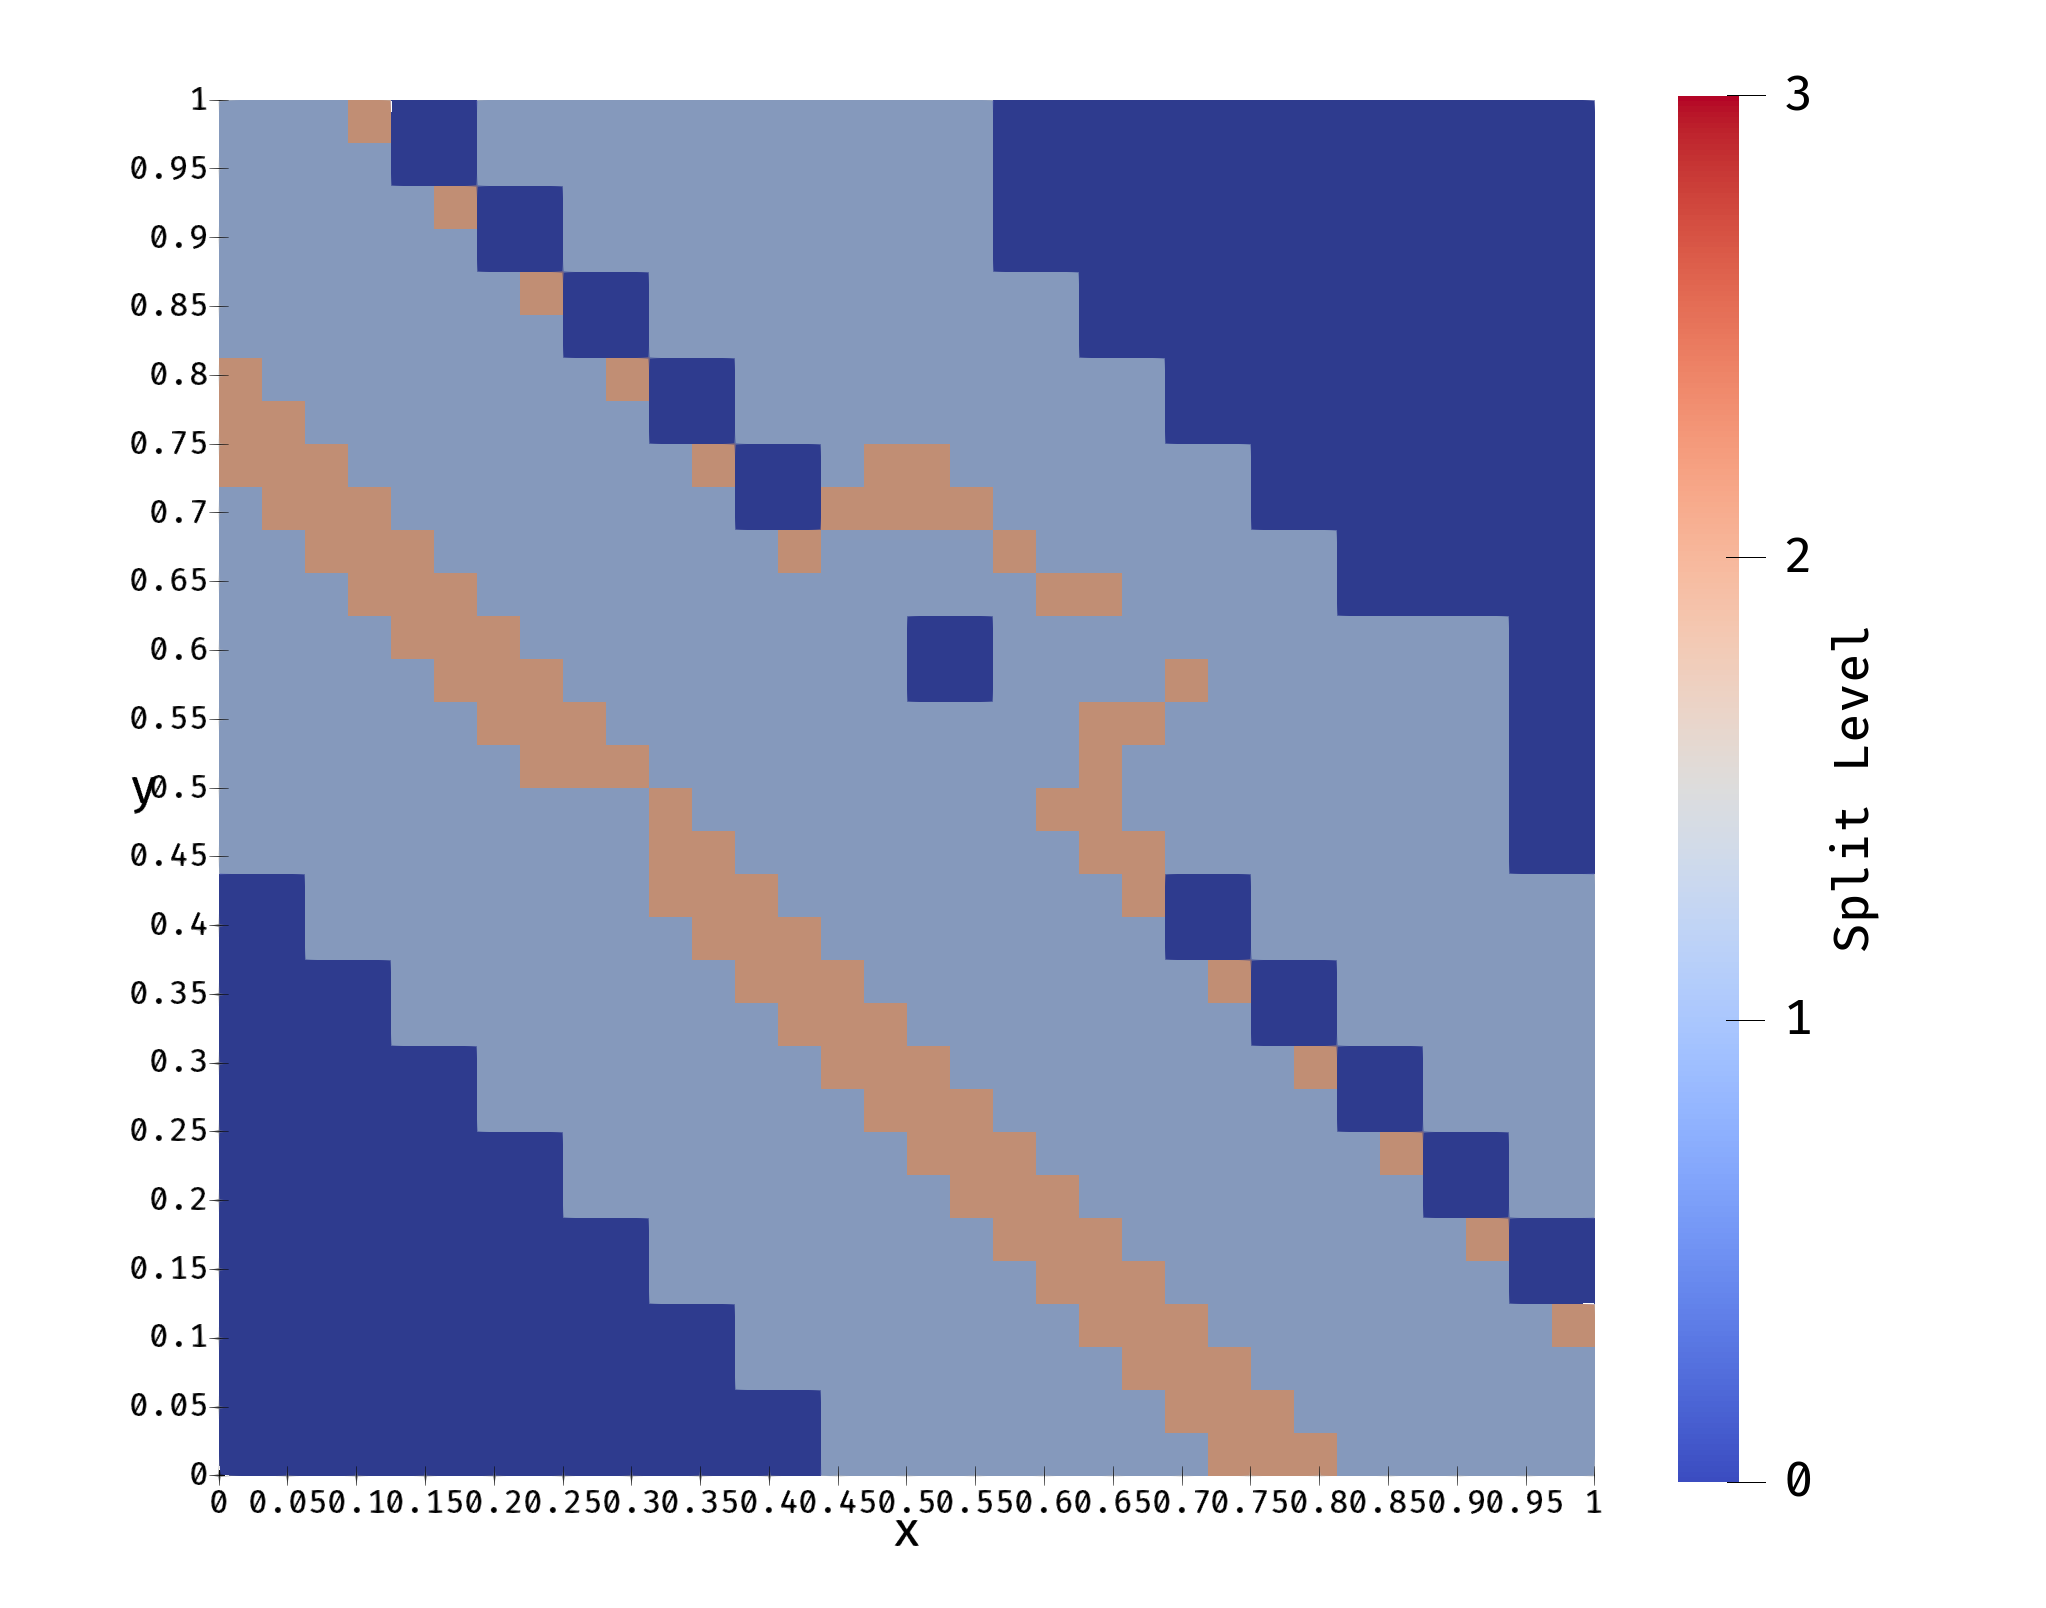
\includegraphics[width=0.48\textwidth]{Chapter_results/media/cloud_split_level_t0}\label{fig:cloud_s_t0}}
    \hfill
    \subfloat[\( t = 0.2 s\)]
    {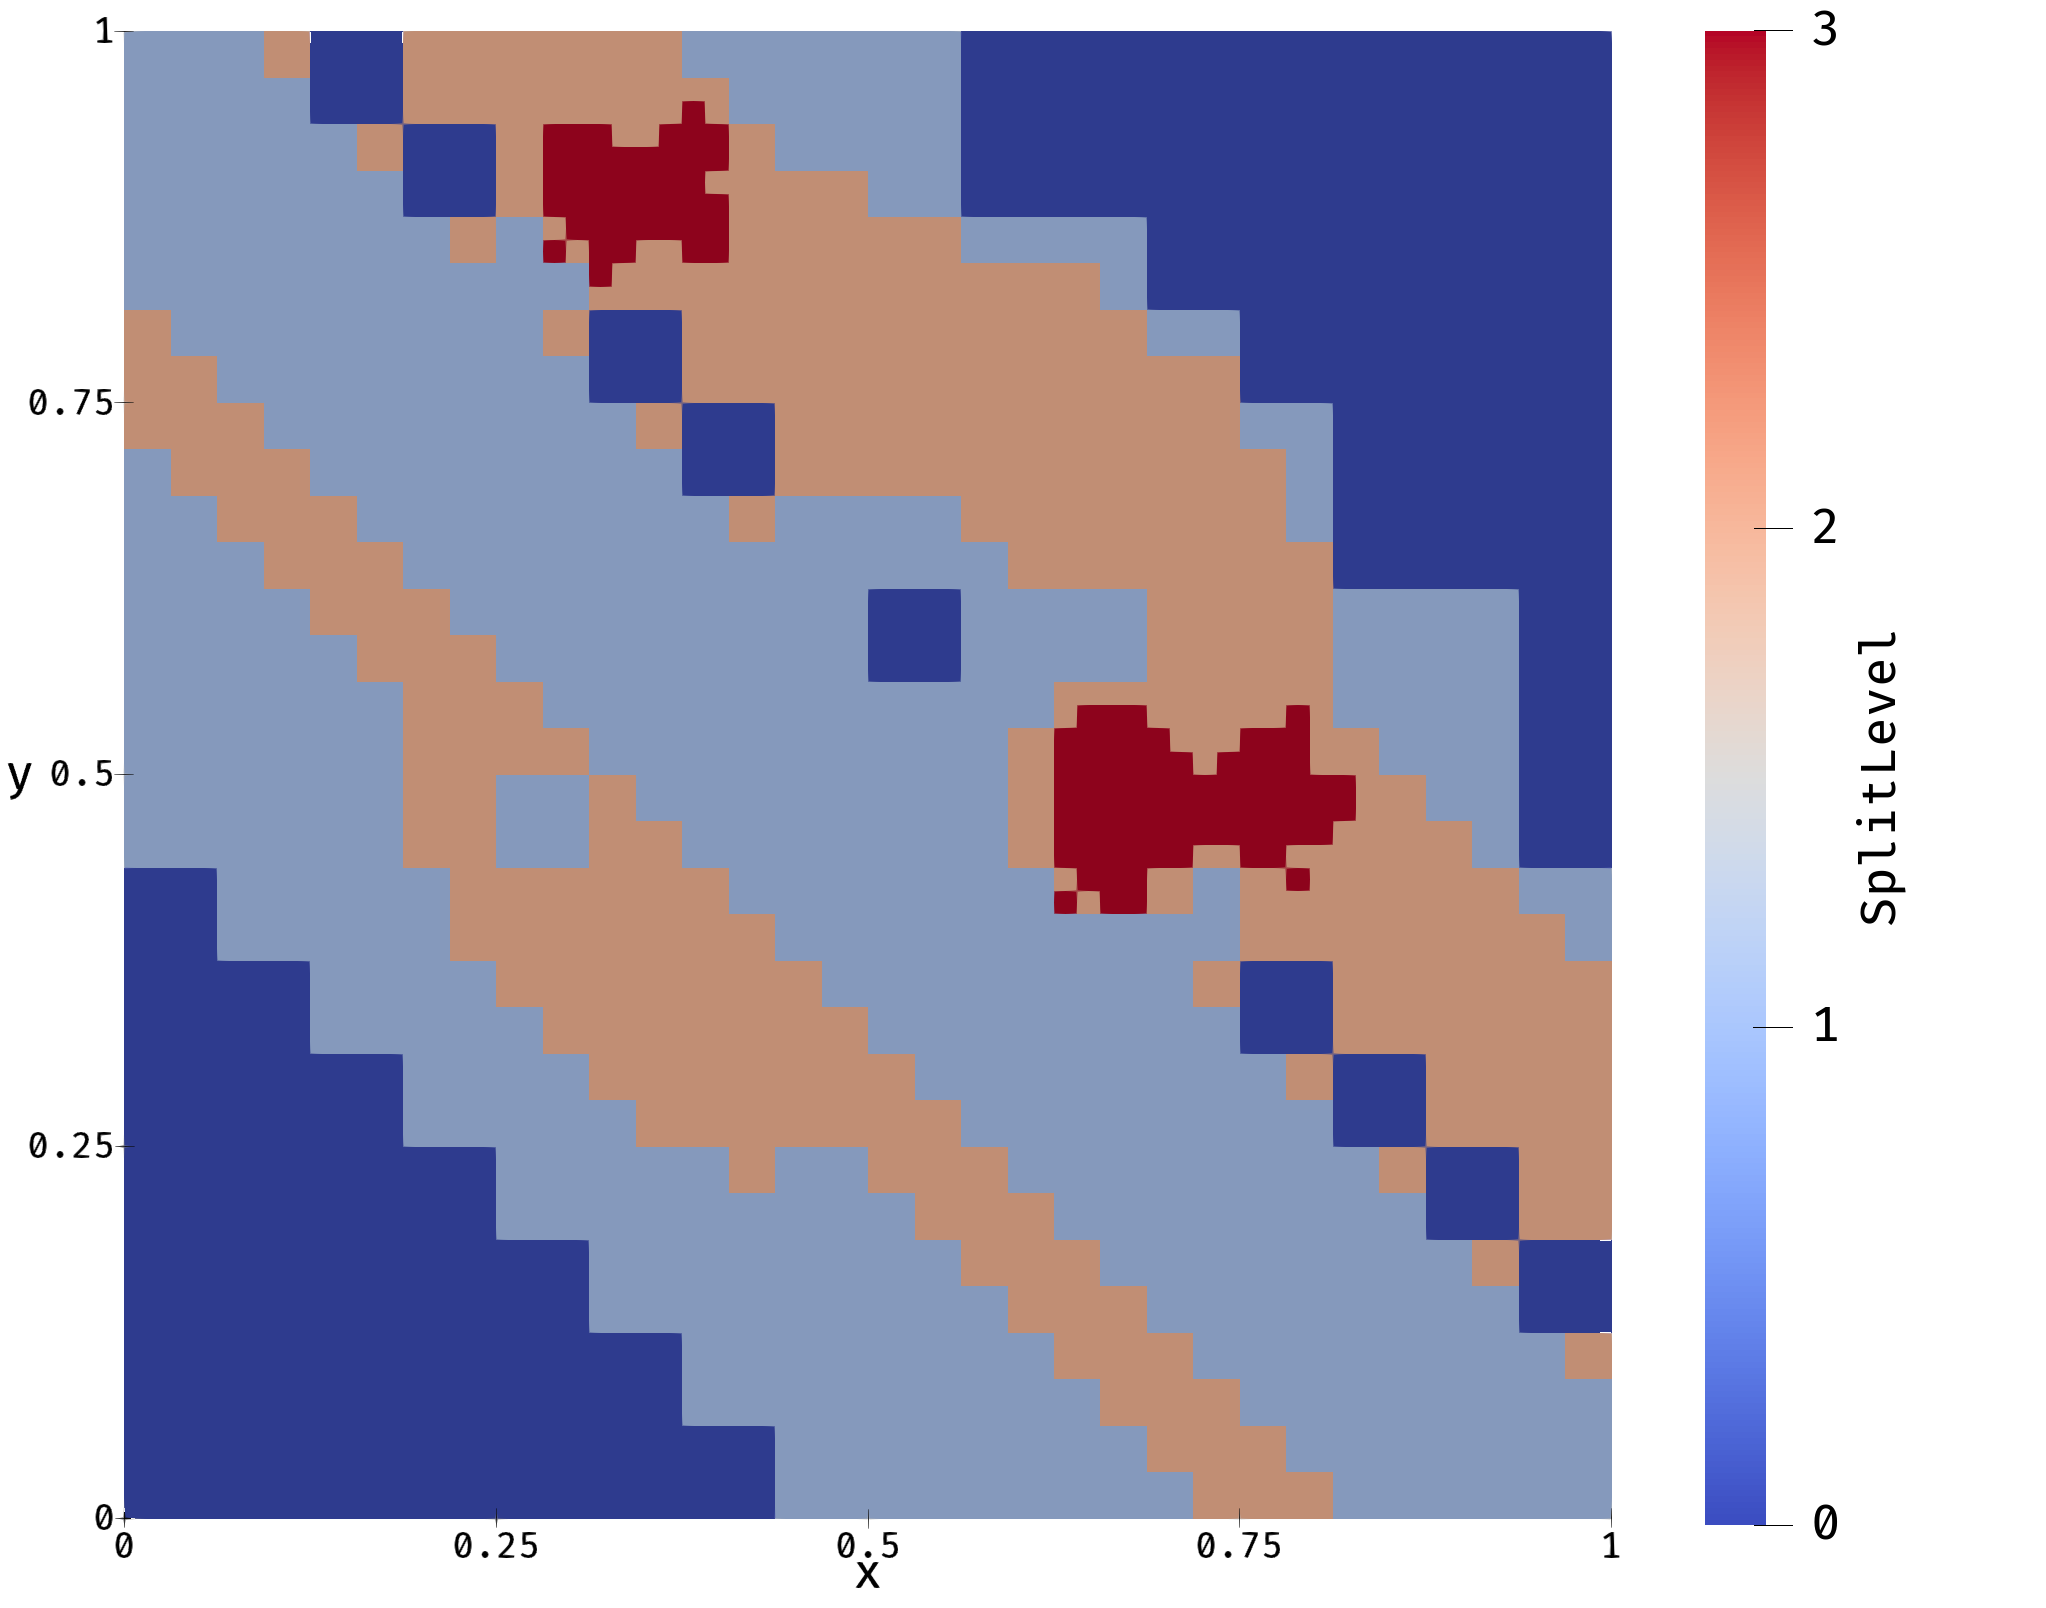
\includegraphics[width=0.48\textwidth]{Chapter_results/media/cloud_split_level_t0_2}\label{fig:cloud_s_t0_2}}
    \caption{Complex case h-refinement: The elements split more where the cloud meets the wave.
        \(N_{initial} = 4\), \(K_{initial} = 256\), \(S = 3\), \(P = 16\) (a) Start of time 
        advancing (b) After the wave and cloud collide}\label{fig:cloud_s}
\end{figure}

\begin{figure}[H]
    \centering
    \subfloat[\( t = 0 s\)]
    {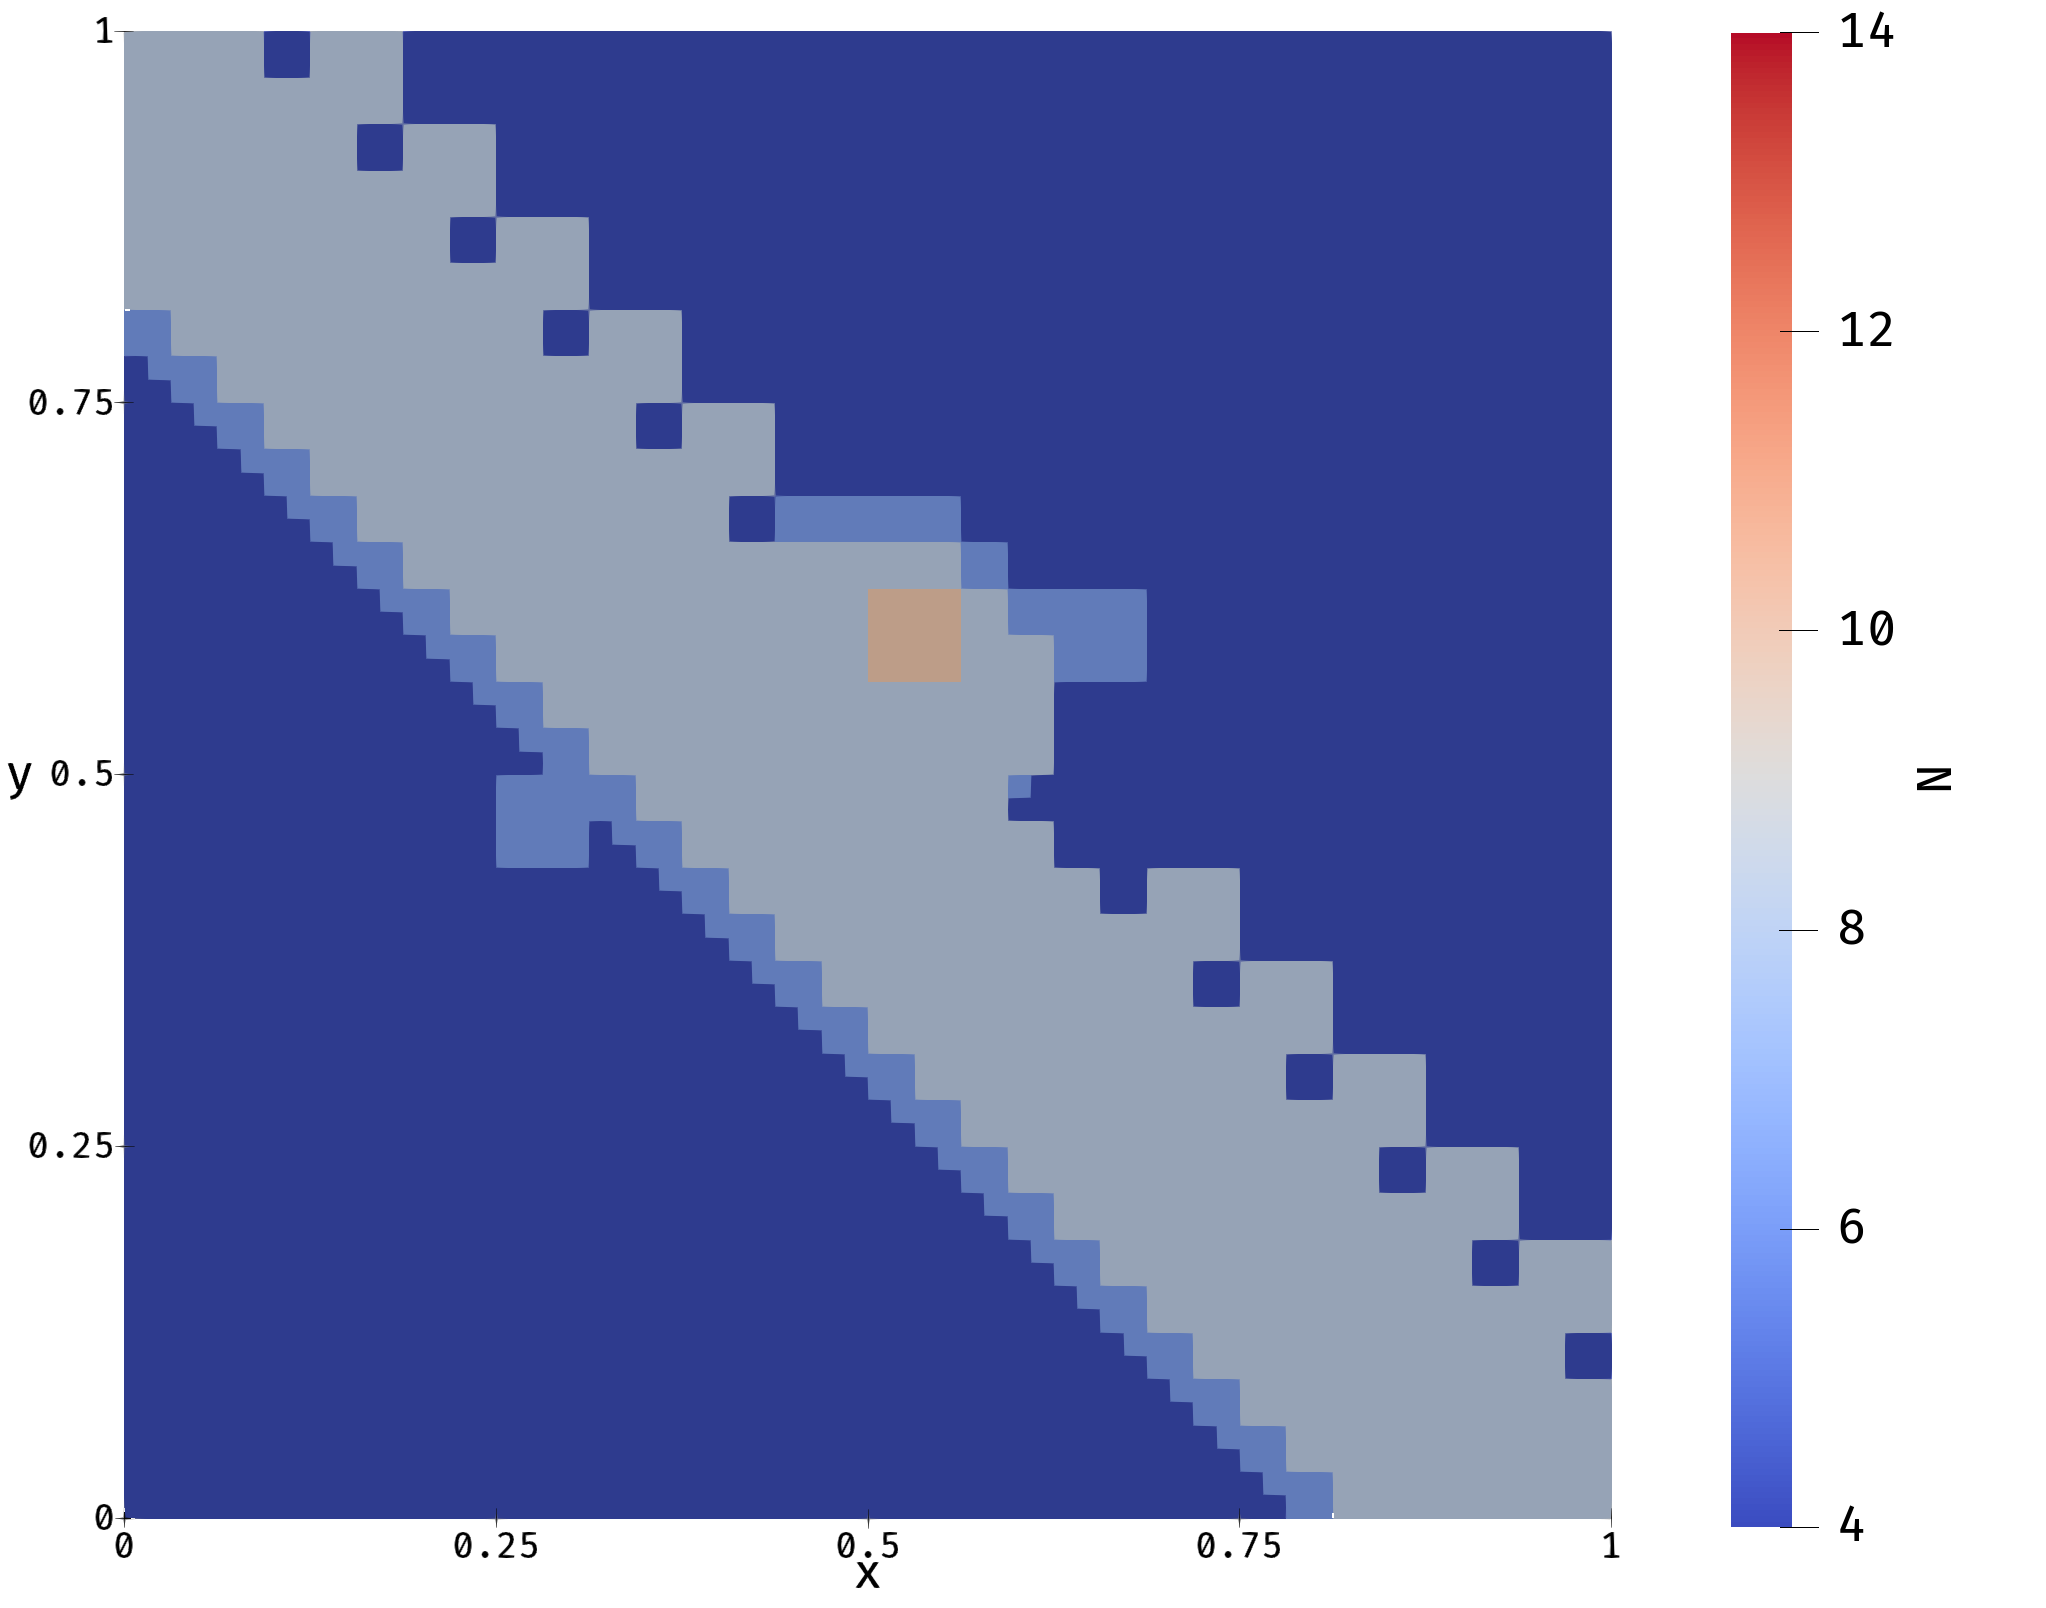
\includegraphics[width=0.48\textwidth]{Chapter_results/media/cloud_N_t0}\label{fig:cloud_N_t0}}
    \hfill
    \subfloat[\( t = 0.2 s\)]
    {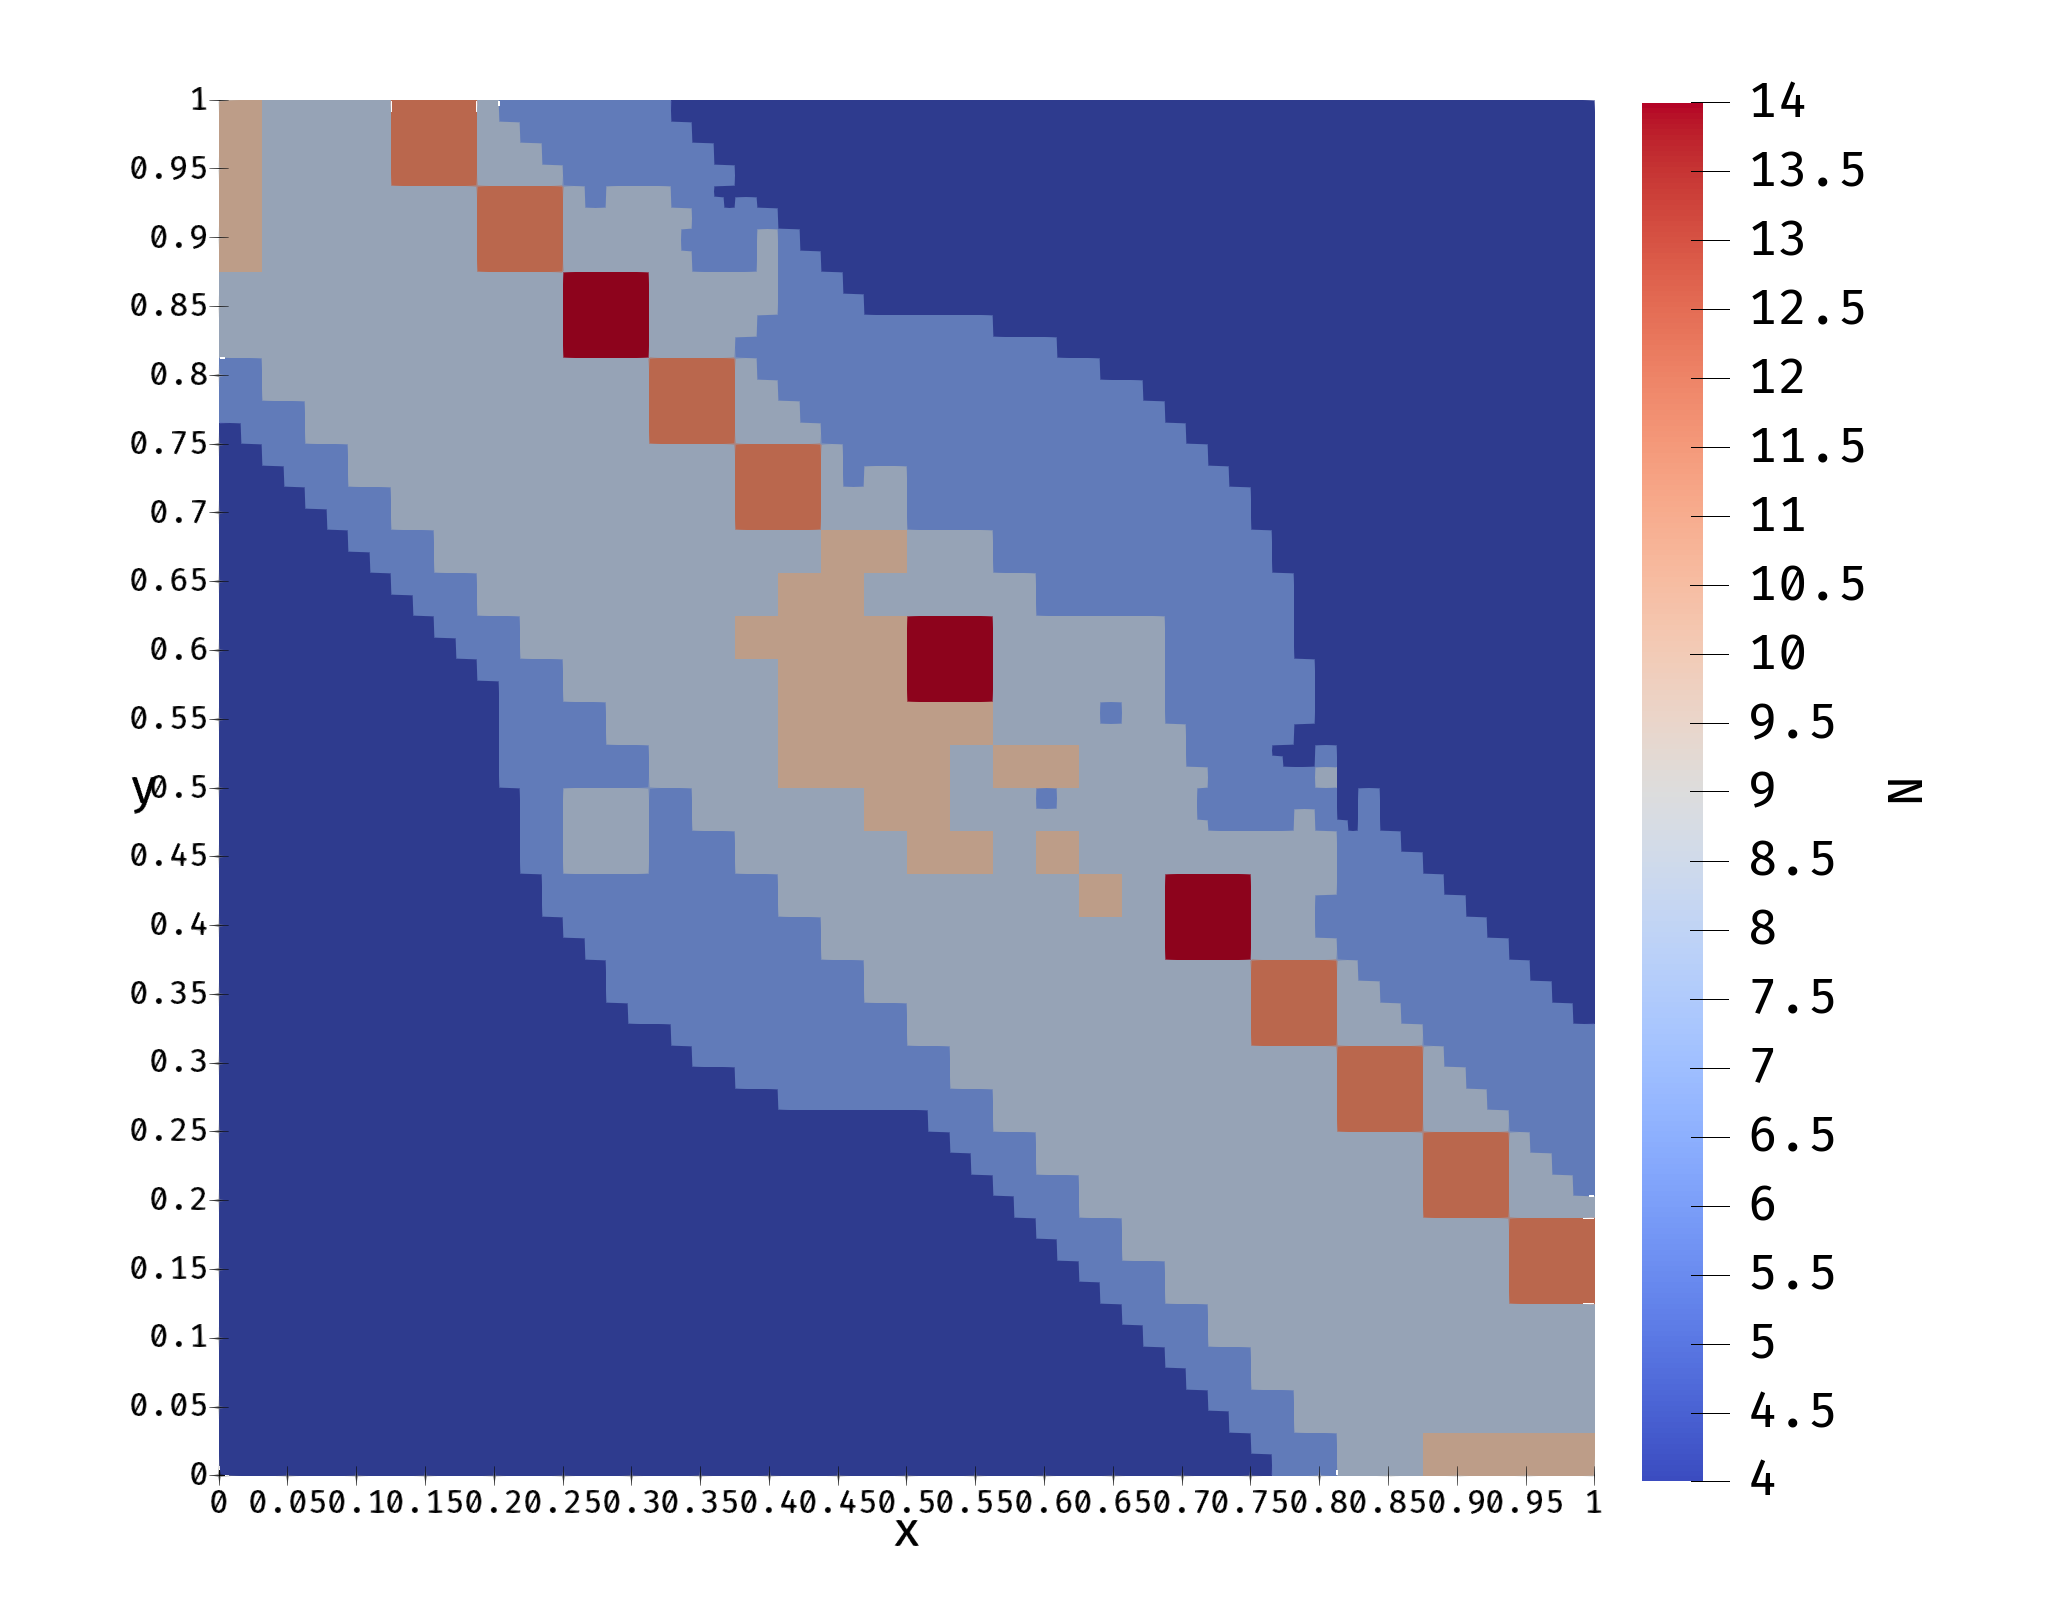
\includegraphics[width=0.48\textwidth]{Chapter_results/media/cloud_N_t0_2}\label{fig:cloud_N_t0_2}}
    \caption{Complex case p-refinement: The polynomial order increases more at the center of the
        cloud and where cloud meets the wave. \(N_{initial} = 4\), \(K_{initial} = 256\), \(S = 3\), 
        \(P = 16\) (a) Start of time advancing (b) After the wave and cloud 
        collide}\label{fig:cloud_N}
\end{figure}

\begin{figure}[H]
    \centering
    \subfloat[\( t = 0 s\)]
    {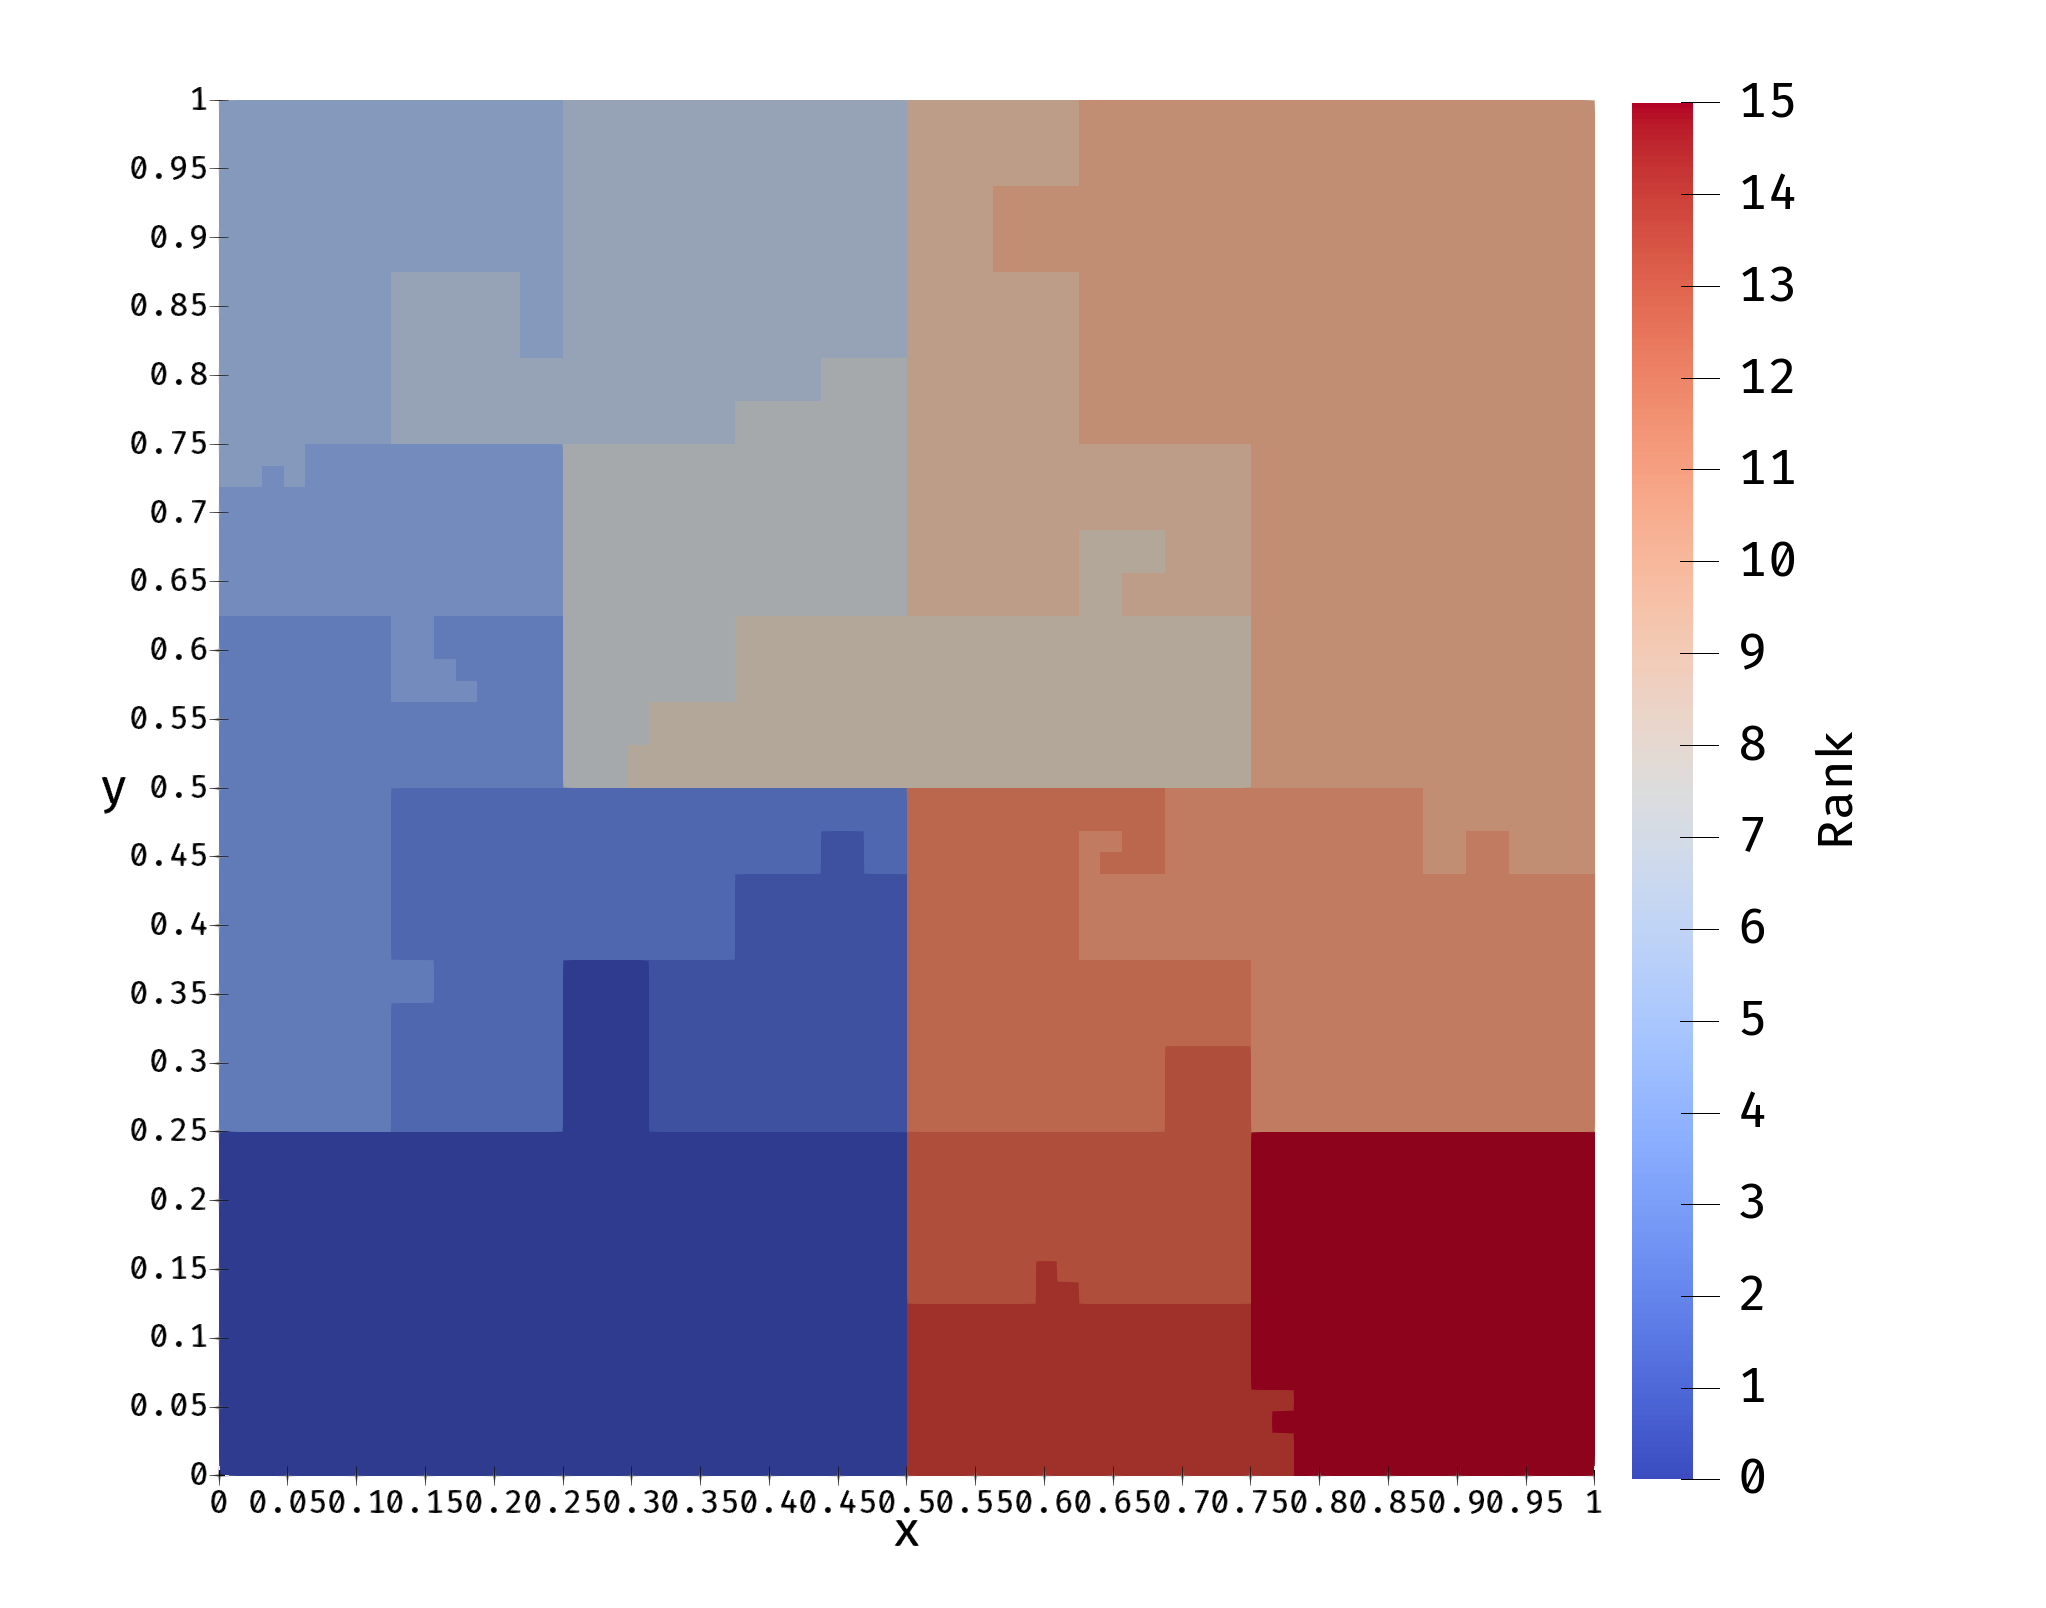
\includegraphics[width=0.48\textwidth]{Chapter_results/media/cloud_rank_t0}\label{fig:cloud_rank_t0}}
    \hfill
    \subfloat[\( t = 0.2 s\)]
    {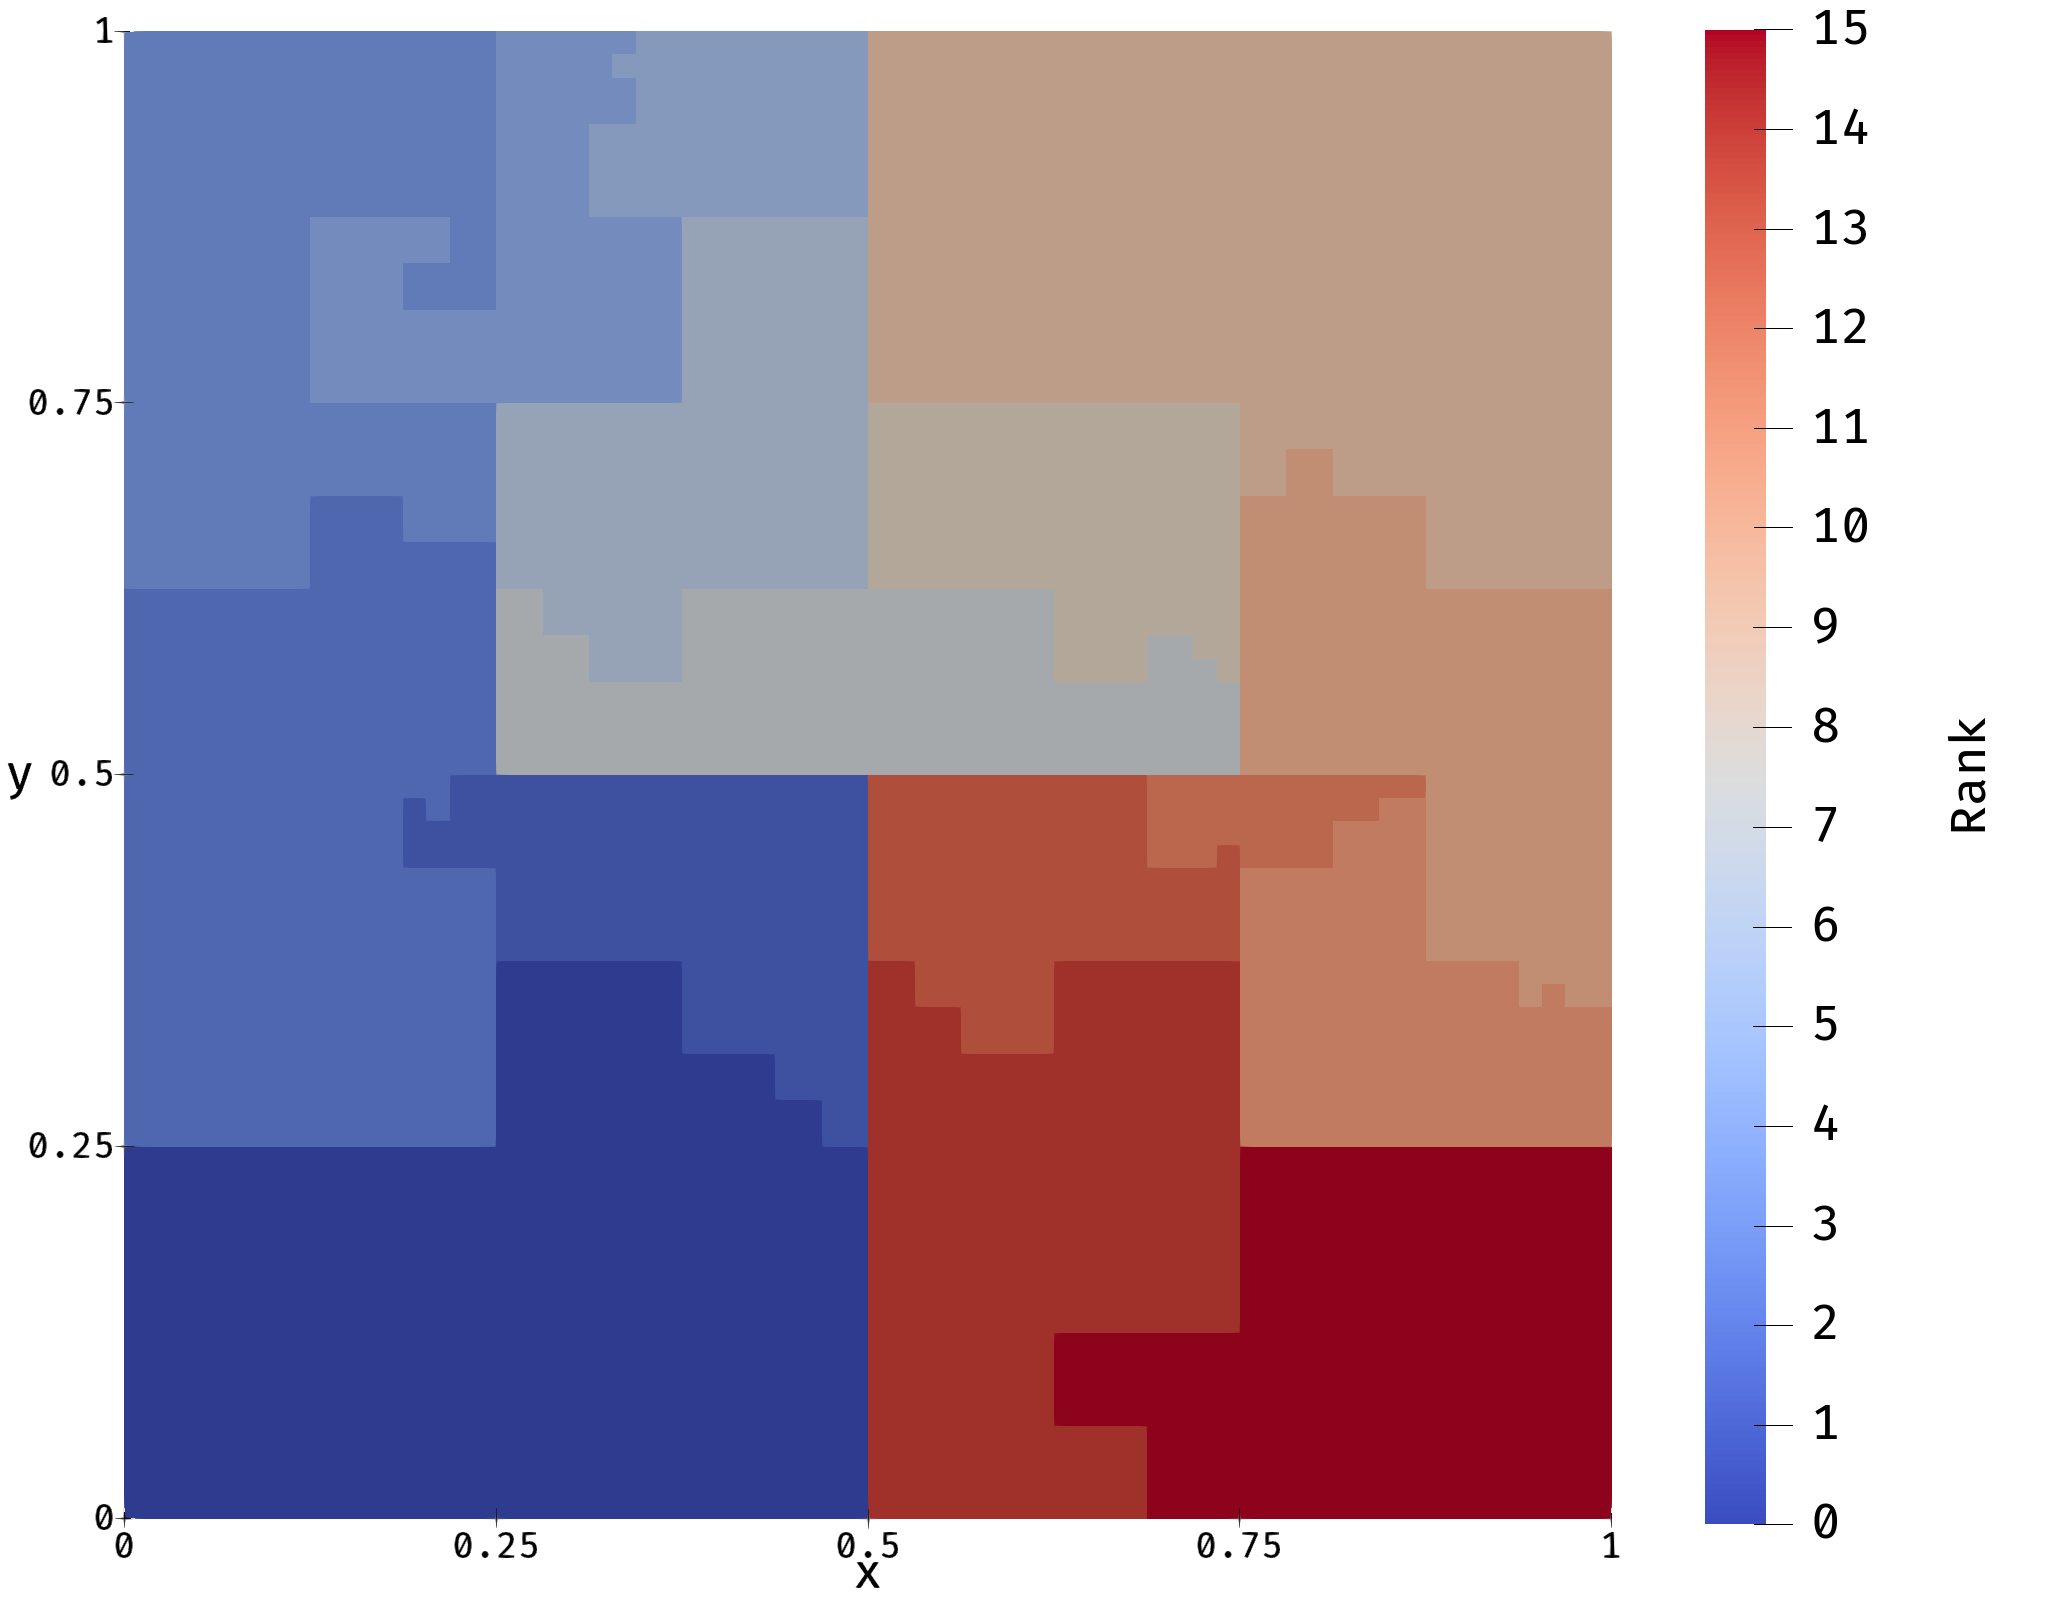
\includegraphics[width=0.48\textwidth]{Chapter_results/media/cloud_rank_t0_2}\label{fig:cloud_rank_t0_2}}
    \caption{Complex case rank: As the mesh is refined load imbalance can occur, and elements are
        sent from one \acrshort{acr:GPU} to another when load balancing. \(N_{initial} = 4\),
        \(K_{initial} = 256\), \(S = 3\), \(P = 16\) (a) Start of time advancing (b) After the wave 
        and cloud collide}\label{fig:cloud_rank}
\end{figure}

These figures show that the pre-condition steps do a good job of refining the mesh to capture the
initial conditions correctly in the \(t = 0 s\) figures (a). Afterwards,
Figures~\ref{fig:cloud_s_t0_2} and~\ref{fig:cloud_N_t0_2} show that the mesh is refined along the
movement of the linear wave and the expansion of the circular cloud, and is especially refined at
their intersection. This indicates that the error estimation correctly identifies the more difficult
areas of the solution. As more elements are created at the intersection of both waves, load
imbalance occurs, and by the end of the computation there are \(K = 5088\) elements. From
Figures~\ref{fig:cloud_s_t0_2} and~\ref{fig:cloud_rank_t0}, we can observe that there are more
h-refining elements around \acrshortpl{acr:GPU} \(6\) and \(8\), which are load balanced by \(t =
0.2 s\) in Figure~\ref{fig:cloud_rank_t0_2}. The elements are moved around by dynamic load
balancing, while keeping good locality and limiting the surface area between \acrshortpl{acr:GPU}.

\section{Complex Meshes}\label{section:results:complex_meshes}

We now introduce a case on a complex geometry to show that the program works with more complex
unstructured meshes that are not axis-aligned. Figure~\ref{fig:complex_mesh} shows the initial mesh
used for this case. Figure~\ref{fig:complex_mesh_pre_condition} shows the adapted mesh and
Figure~\ref{fig:complex_mesh_solution_p} depicts a wave moving across a NACA 0012 airfoil inside a
circular domain of radius \(20\). The mesh initially has \(K = 2128\) elements, is allowed to
h-refine up to \(S = 3\), and by the end of the computation there are \(K = 55680\) elements. The
polynomial order of the elements is initially \(N = 4\) and is allowed to p-refine up to \(N = 16\).
The mesh is refined every \(1000\) timesteps and load balanced with a imbalance threshold of \(L =
1.1\). At the beginning of the computation, three pre-condition steps are performed, which is why
the mesh is already refined at \(t = 0 s\) in Figure~\ref{fig:complex_mesh_pre_condition_far}. The
solution is computed in parallel on \(P = 4\) \acrshortpl{acr:GPU}.

The mesh is unstructured, and the original mesh file is numbered in a way that places elements with
neighbouring indices very far apart in the 2D domain. This is not ideal, as it scatters memory
accesses in a way that is detrimental to \acrshort{acr:GPU} performance, and increases dramatically
the number of inter-\acrshort{acr:GPU} boundaries. To improve the numbering, the mesh was renumbered
to a pseudo-Hilbert curve according to an algorithm presented in Appendix~\ref{chapter:renumbering}.
It is not a real Hilbert curve, as the Hilbert curve is only defined in 2D square domains with a
power of two number of axis-aligned elements in both dimensions. Nonetheless, this pseudo-Hilbert
curve resembles the Hilbert curve, and improves locality.

\begin{figure}[H]
    \centering
    \subfloat[Circular domain]
    {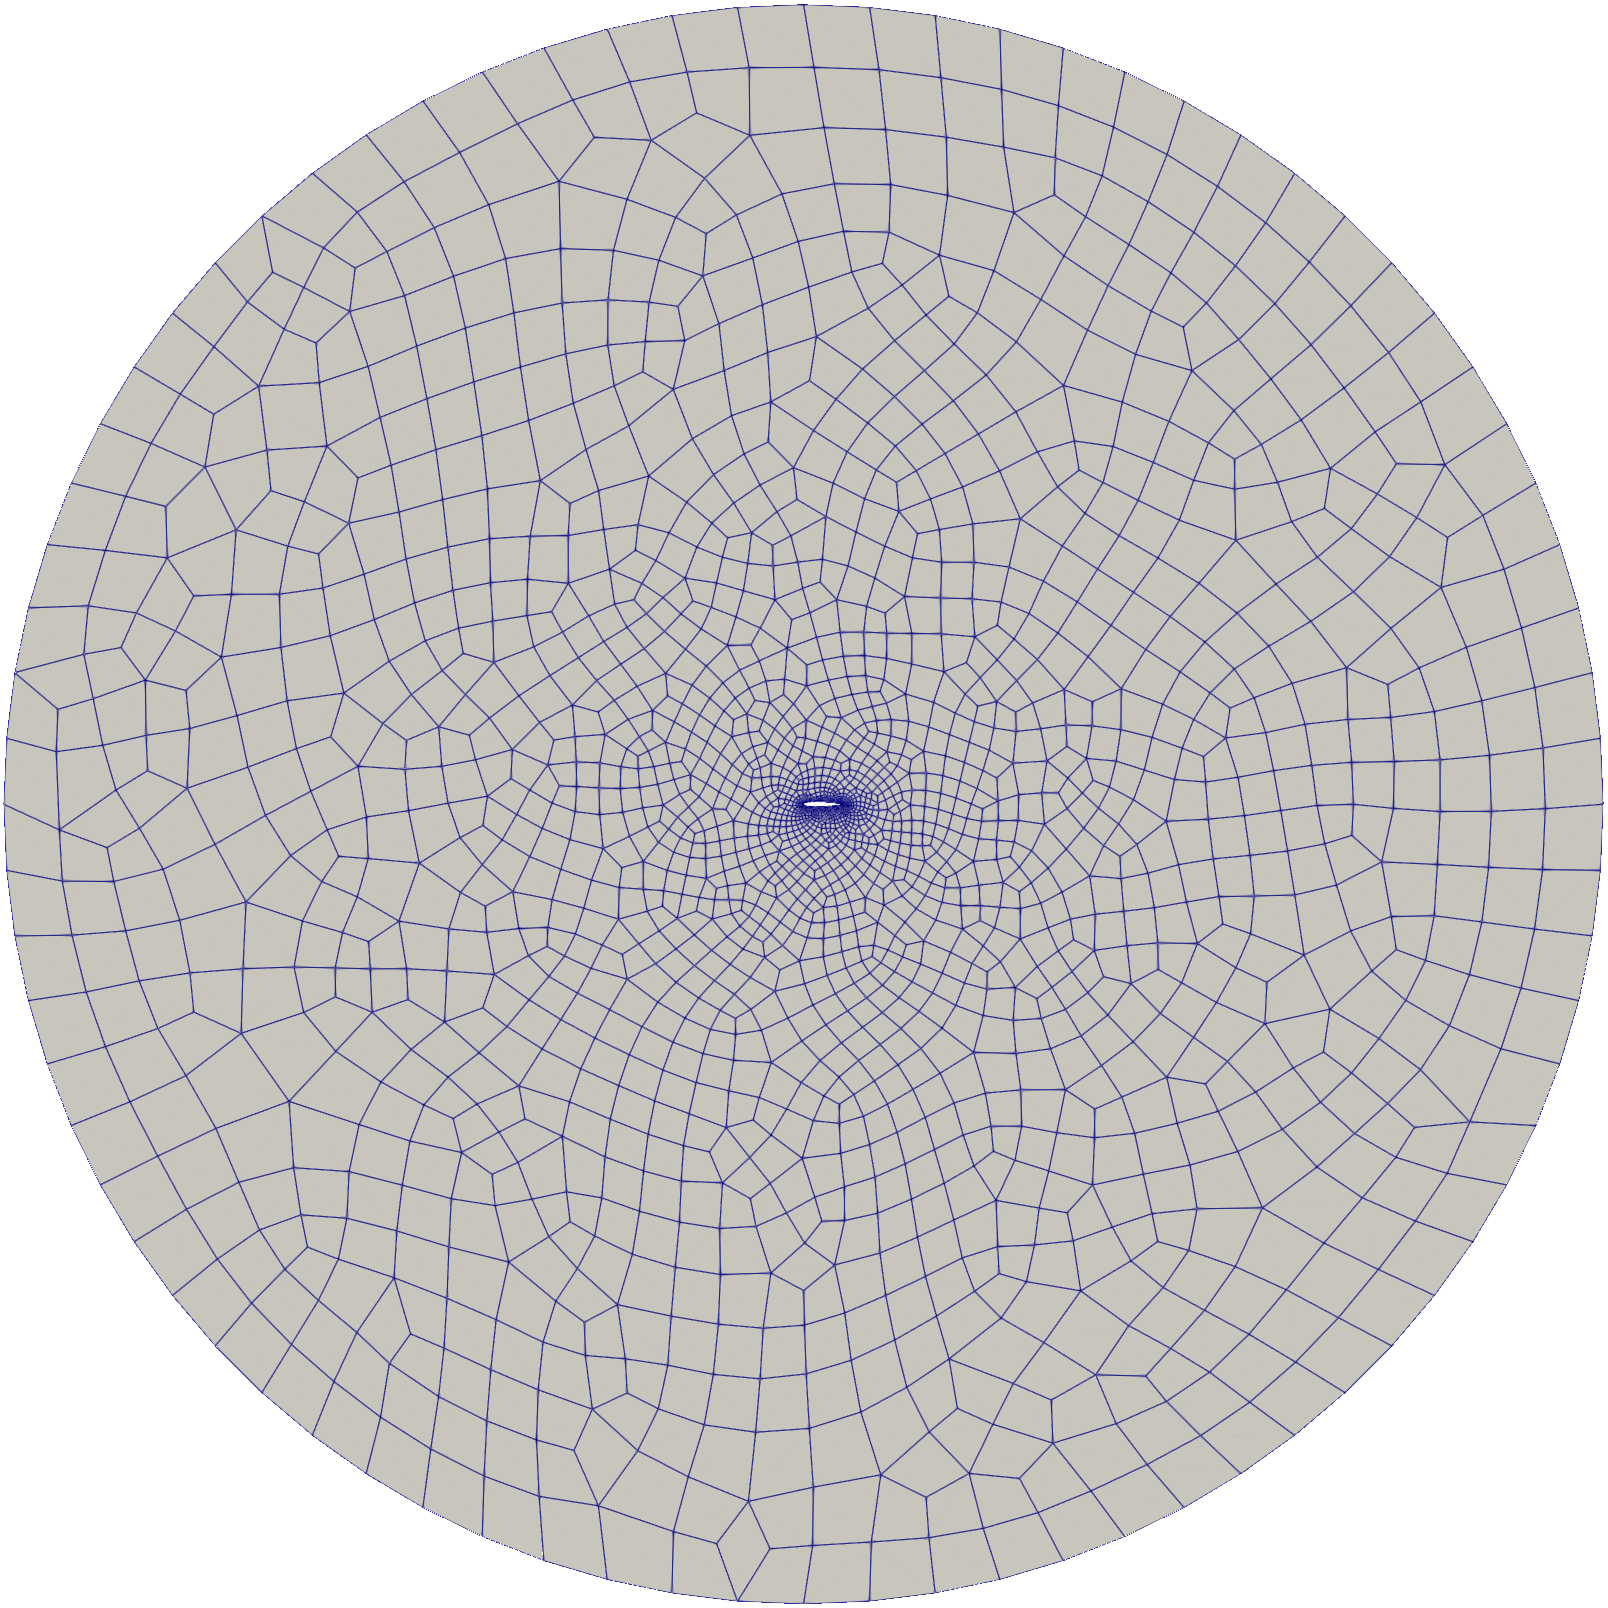
\includegraphics[width=0.48\textwidth]{Chapter_results/media/airfoil_mesh_far}\label{fig:complex_mesh_far}}
    \hfill
    \subfloat[Airfoil]
    {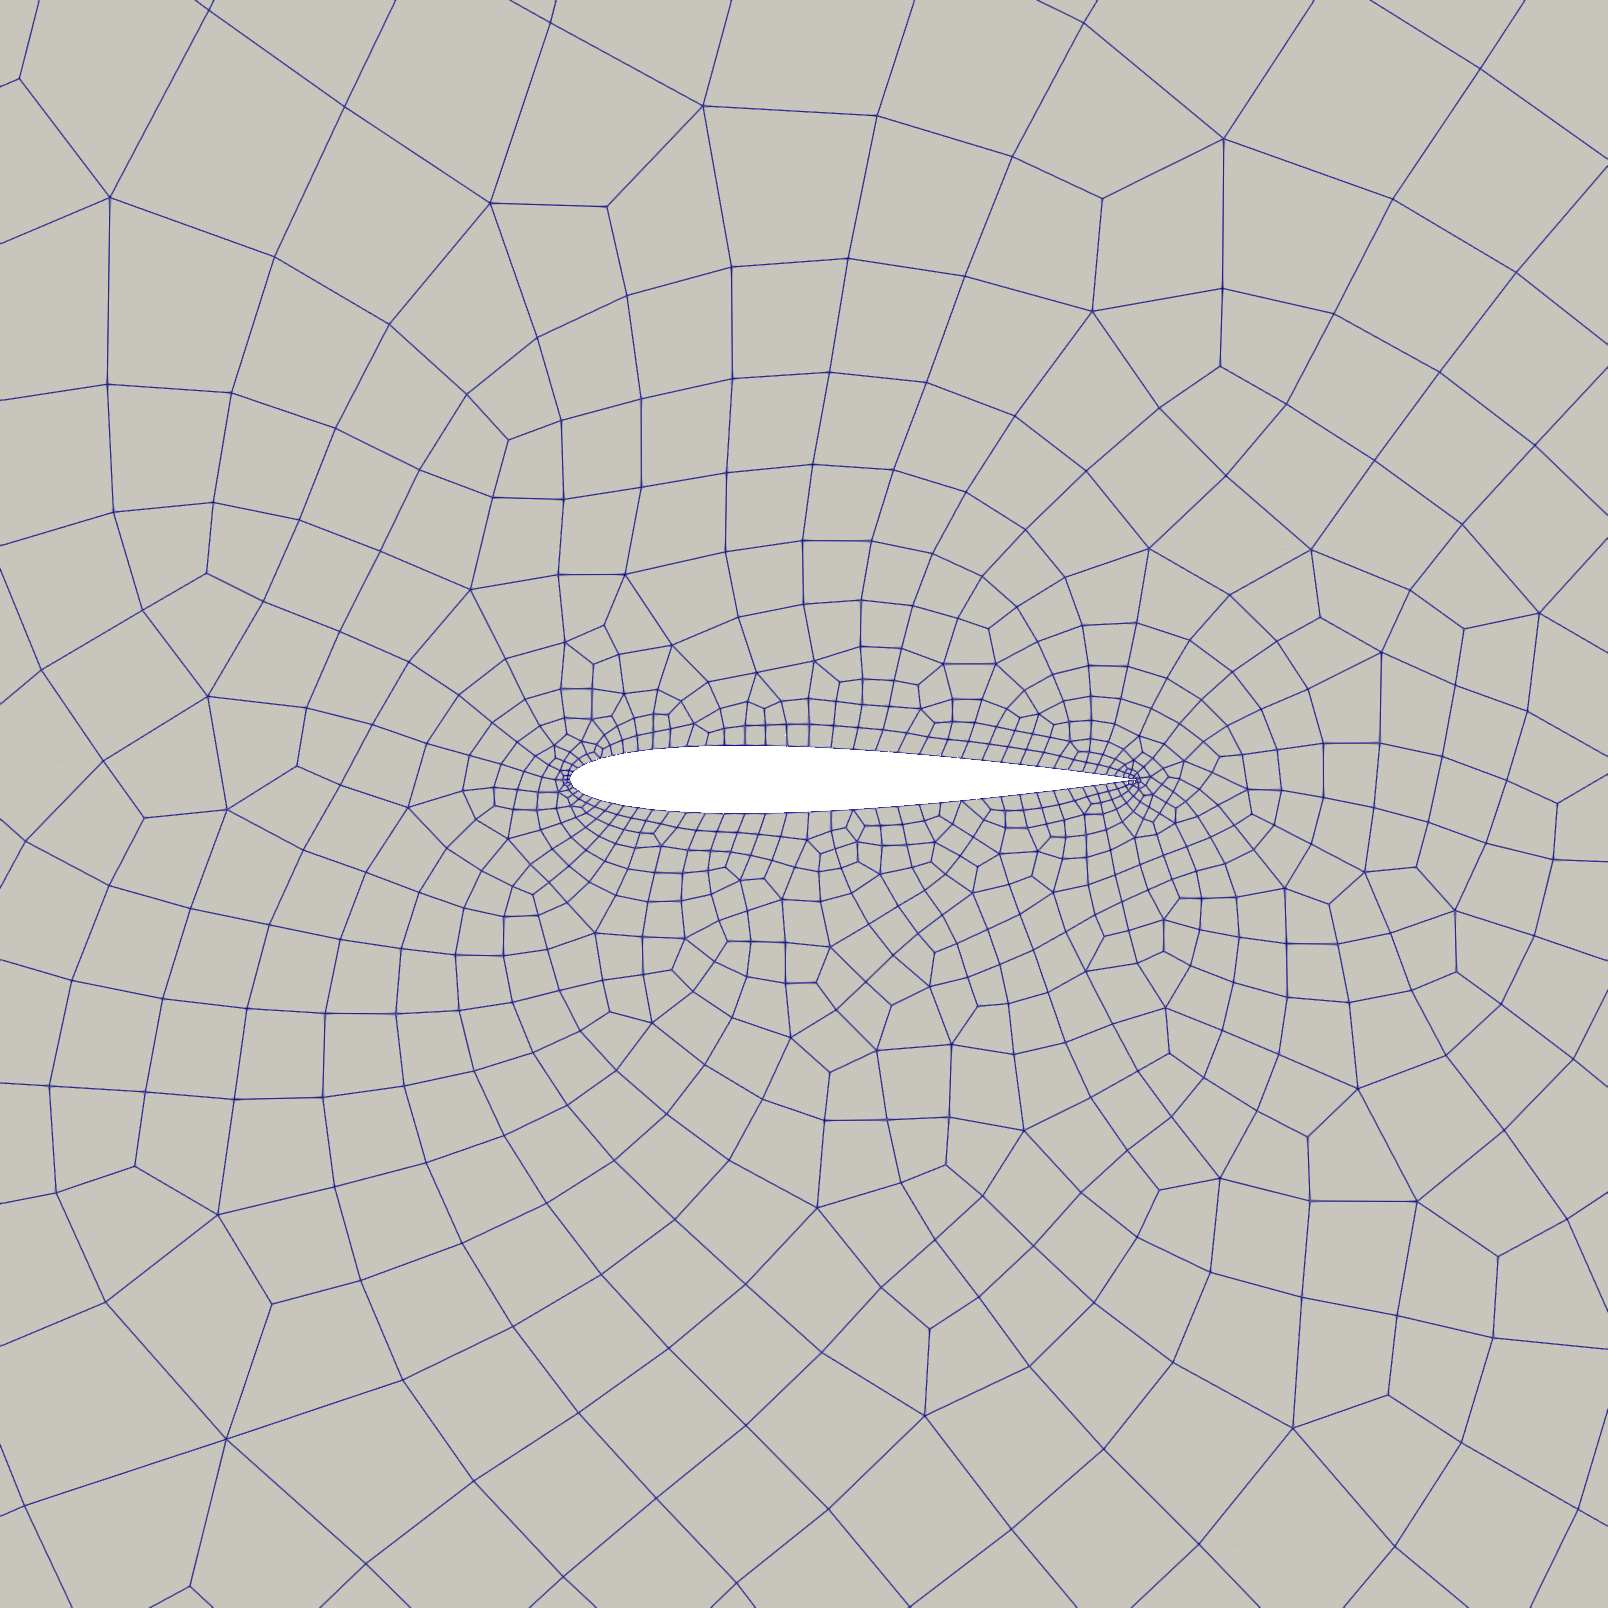
\includegraphics[width=0.48\textwidth]{Chapter_results/media/airfoil_mesh_near}\label{fig:complex_mesh_near}}
    \caption{Complex mesh example: An airfoil in an unstructured circular domain with its initial 
        mesh. \(N_{initial} = 4\), \(K_{initial} = 2128\), \(S = 3\), \(P = 4\) (a) Complete domain 
        (b) Up close}\label{fig:complex_mesh}
\end{figure}

\begin{figure}[H]
    \centering
    \subfloat[Circular domain]
    {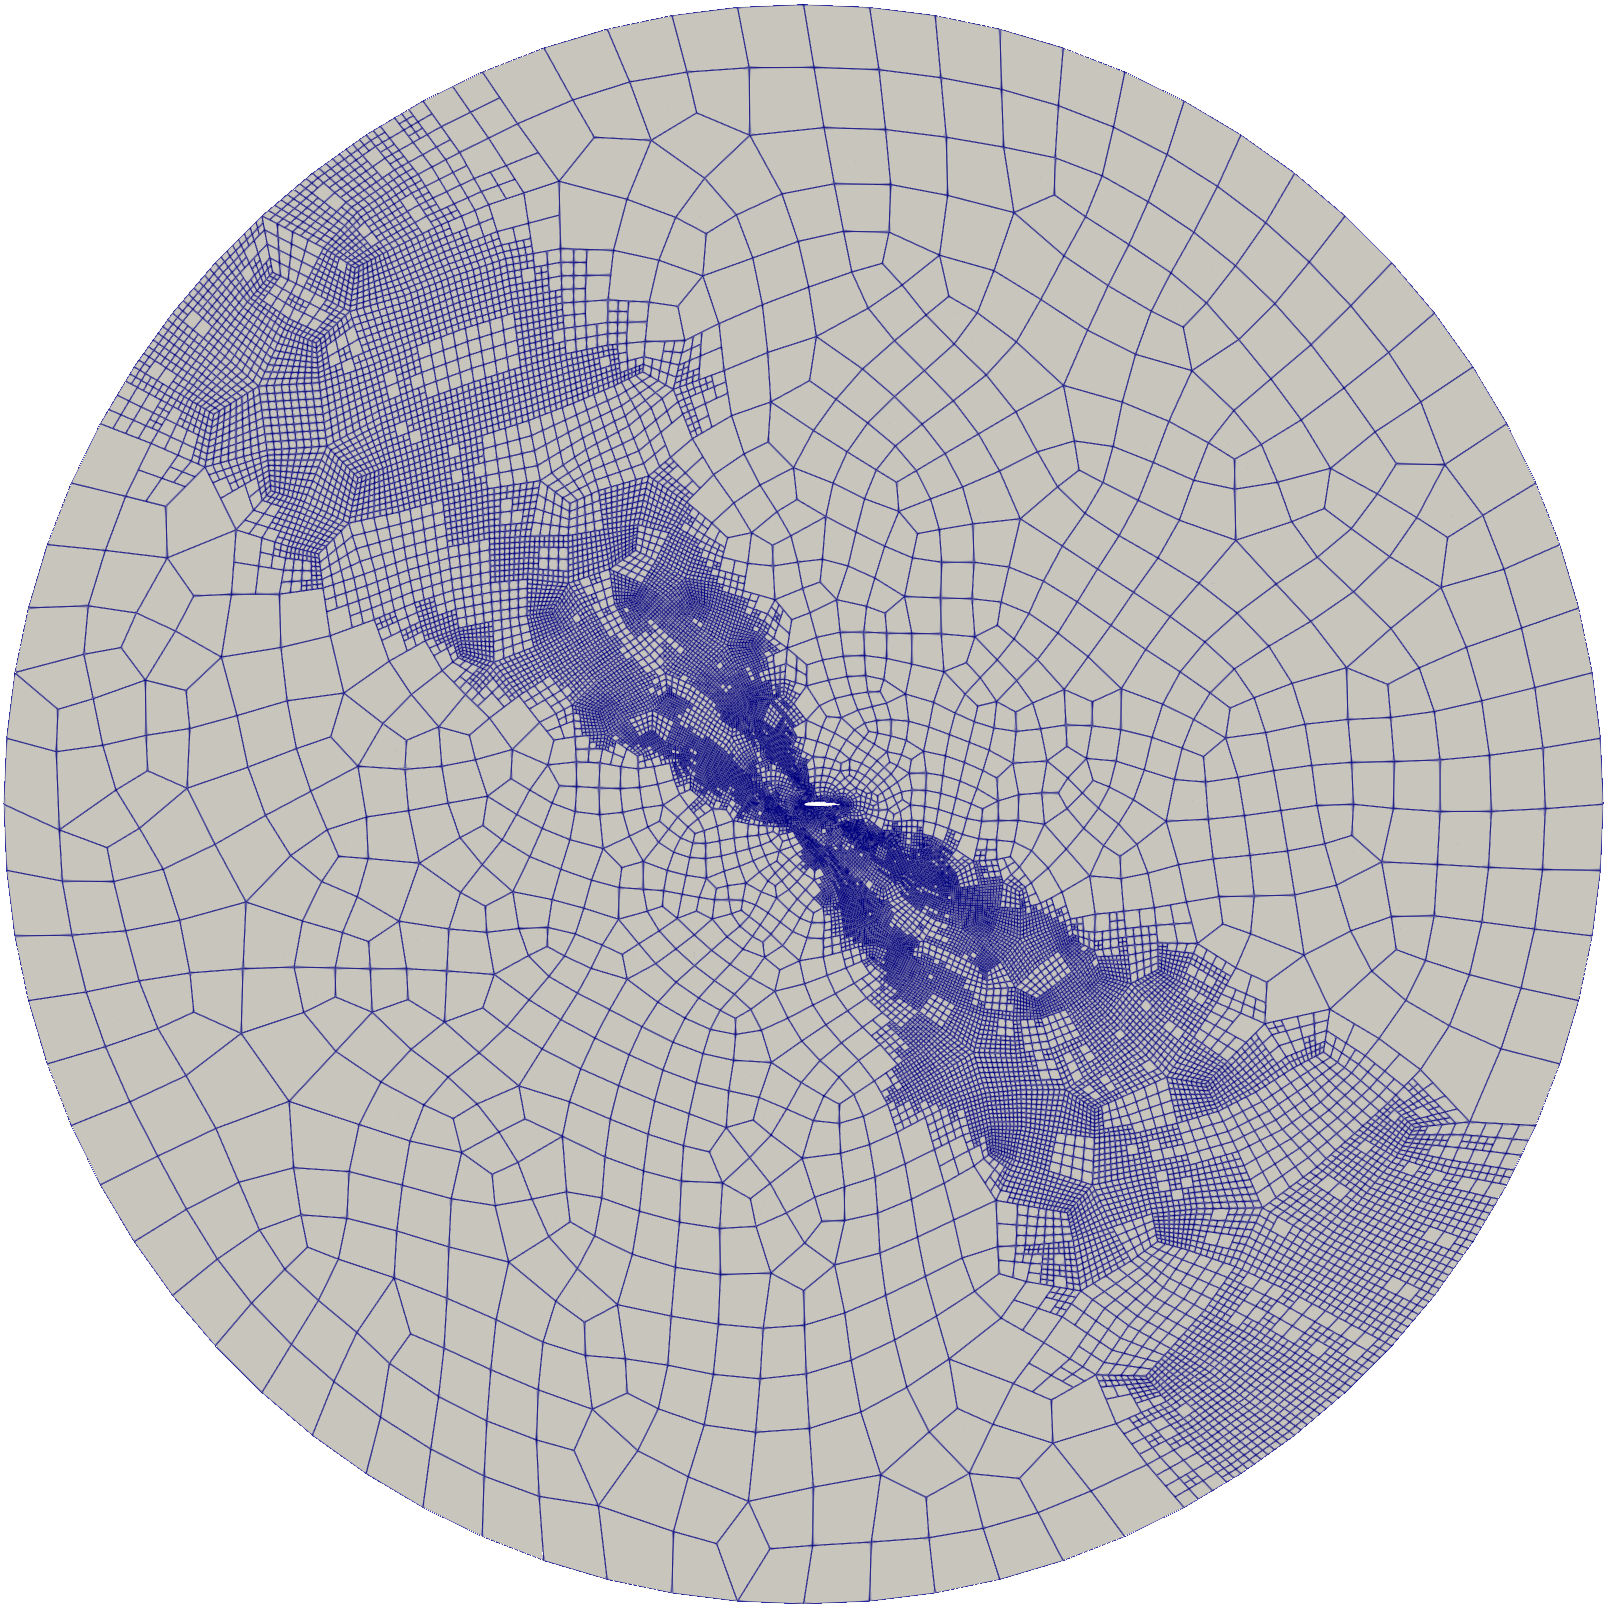
\includegraphics[width=0.48\textwidth]{Chapter_results/media/airfoil_mesh_pre_condition_far}\label{fig:complex_mesh_pre_condition_far}}
    \hfill
    \subfloat[Airfoil]
    {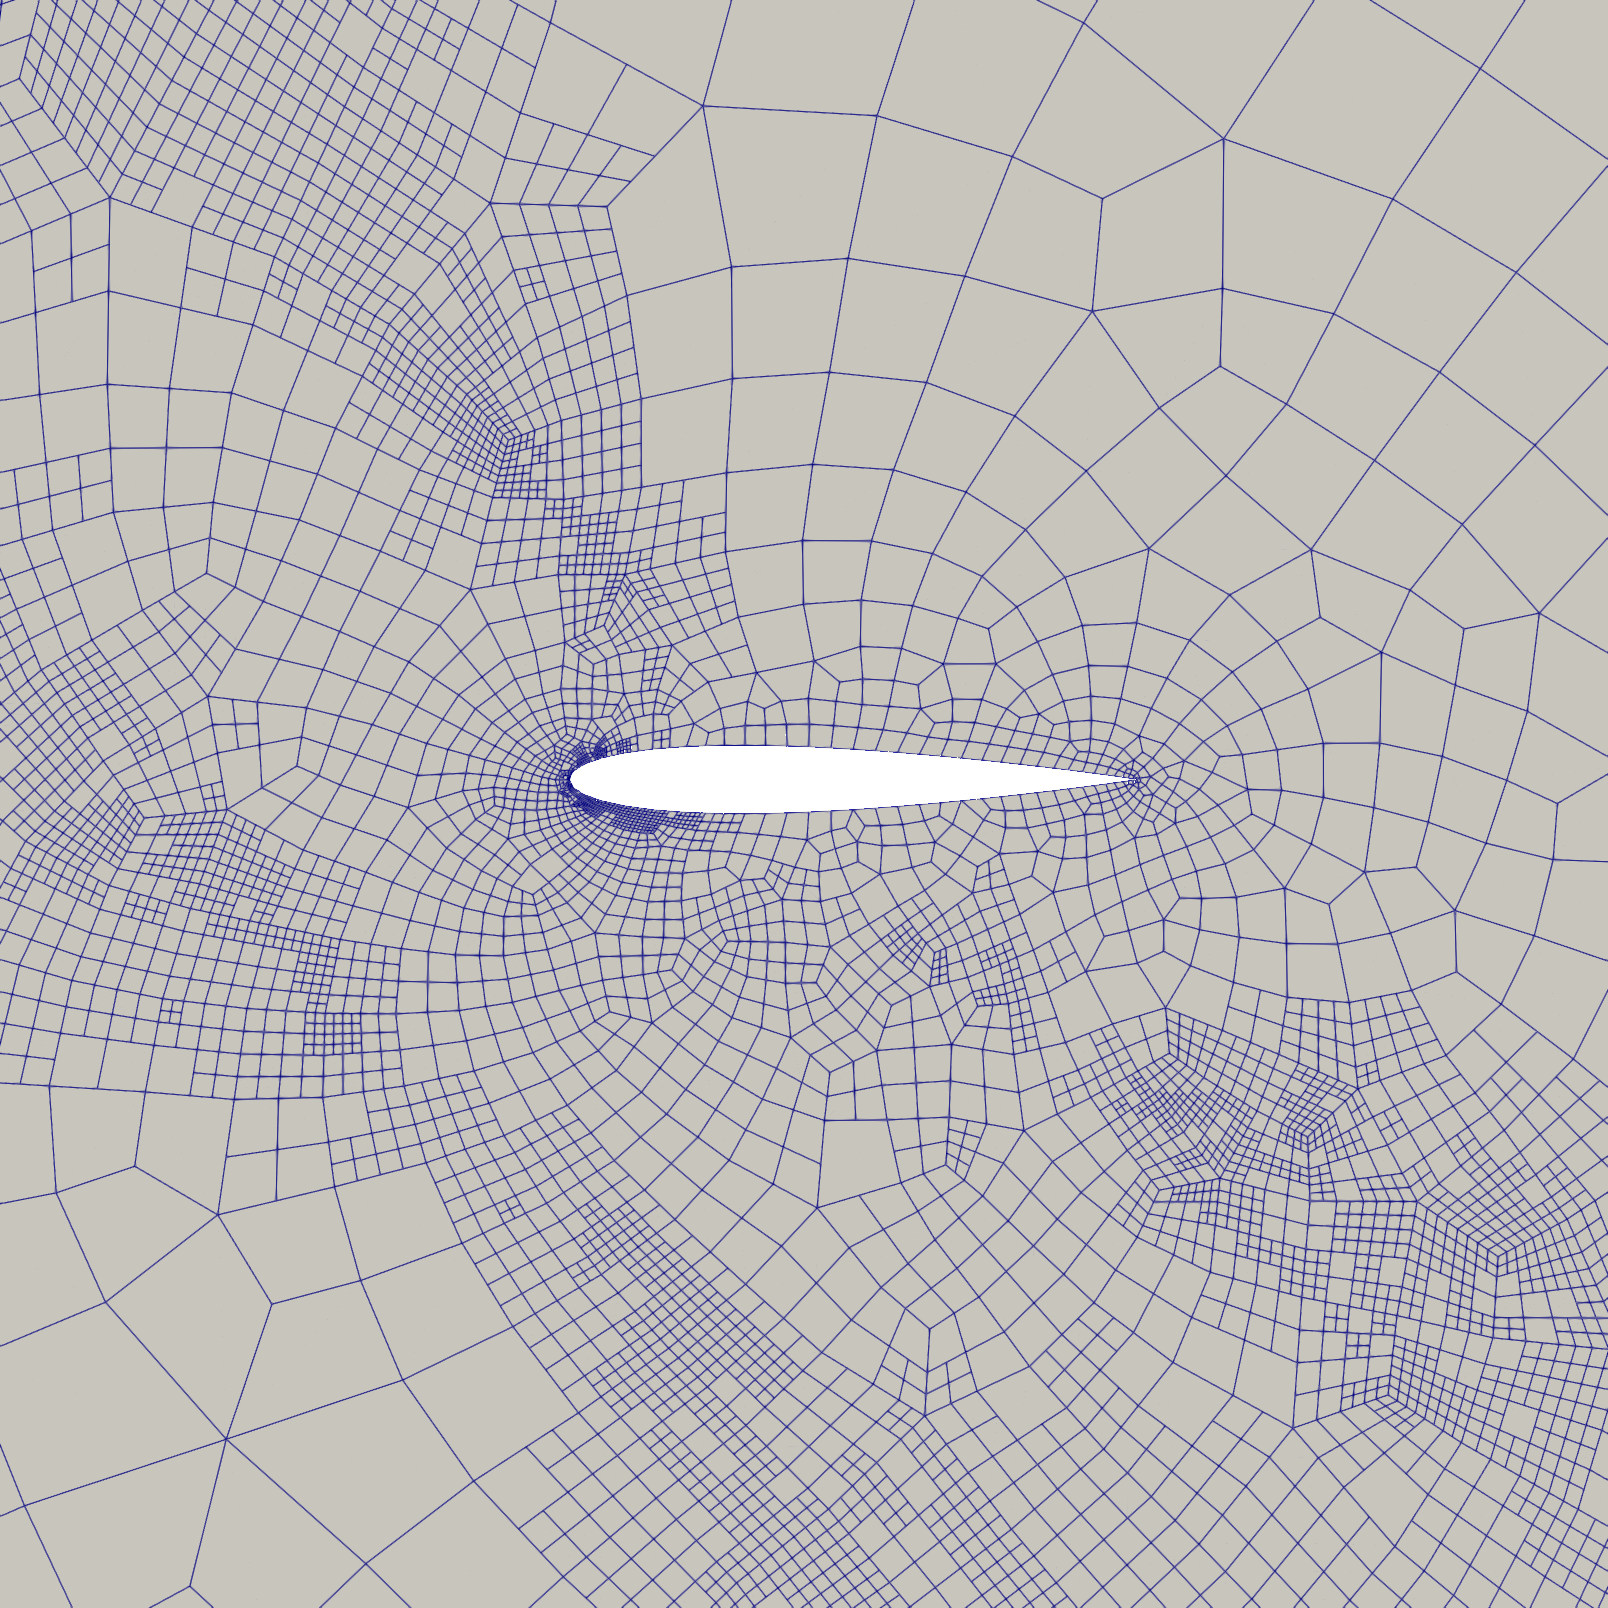
\includegraphics[width=0.48\textwidth]{Chapter_results/media/airfoil_mesh_pre_condition_near}\label{fig:complex_mesh_pre_condition_near}}
    \caption{Complex mesh after pre-condition: Elements have been added to better apply initial 
        conditions. \(N_{initial} = 4\), \(K = 24072\), \(S = 3\), \(P = 4\) (a) Complete domain (b) 
        Up close}\label{fig:complex_mesh_pre_condition}
\end{figure}

Figure~\ref{fig:complex_mesh_solution} shows the problem after \(1.5\) seconds of solution time.
Figure~\ref{fig:complex_mesh_solution_p} shows the pressure distribution, the wave having passed
around the airfoil and created a reflected circular wave.
Figure~\ref{fig:complex_mesh_solution_sigma} shows the pressure error decay rate \(\sigma \), which
informs the decision between h-refinement and p-refinement. An orange value, above \(1\), indicates
p-refinement would be chosen, whereas a blue value, below \(1\), indicates h-refinement would be
chosen. Figure~\ref{fig:complex_mesh_split_level} shows the split level \(S\), denoting how many
times elements have h-refined. Figure~\ref{fig:complex_mesh_N} shows the polynomial order \(N\),
which increases when elements are p-refined.

\begin{figure}[H]
    \centering

    \subfloat[Pressure]
    {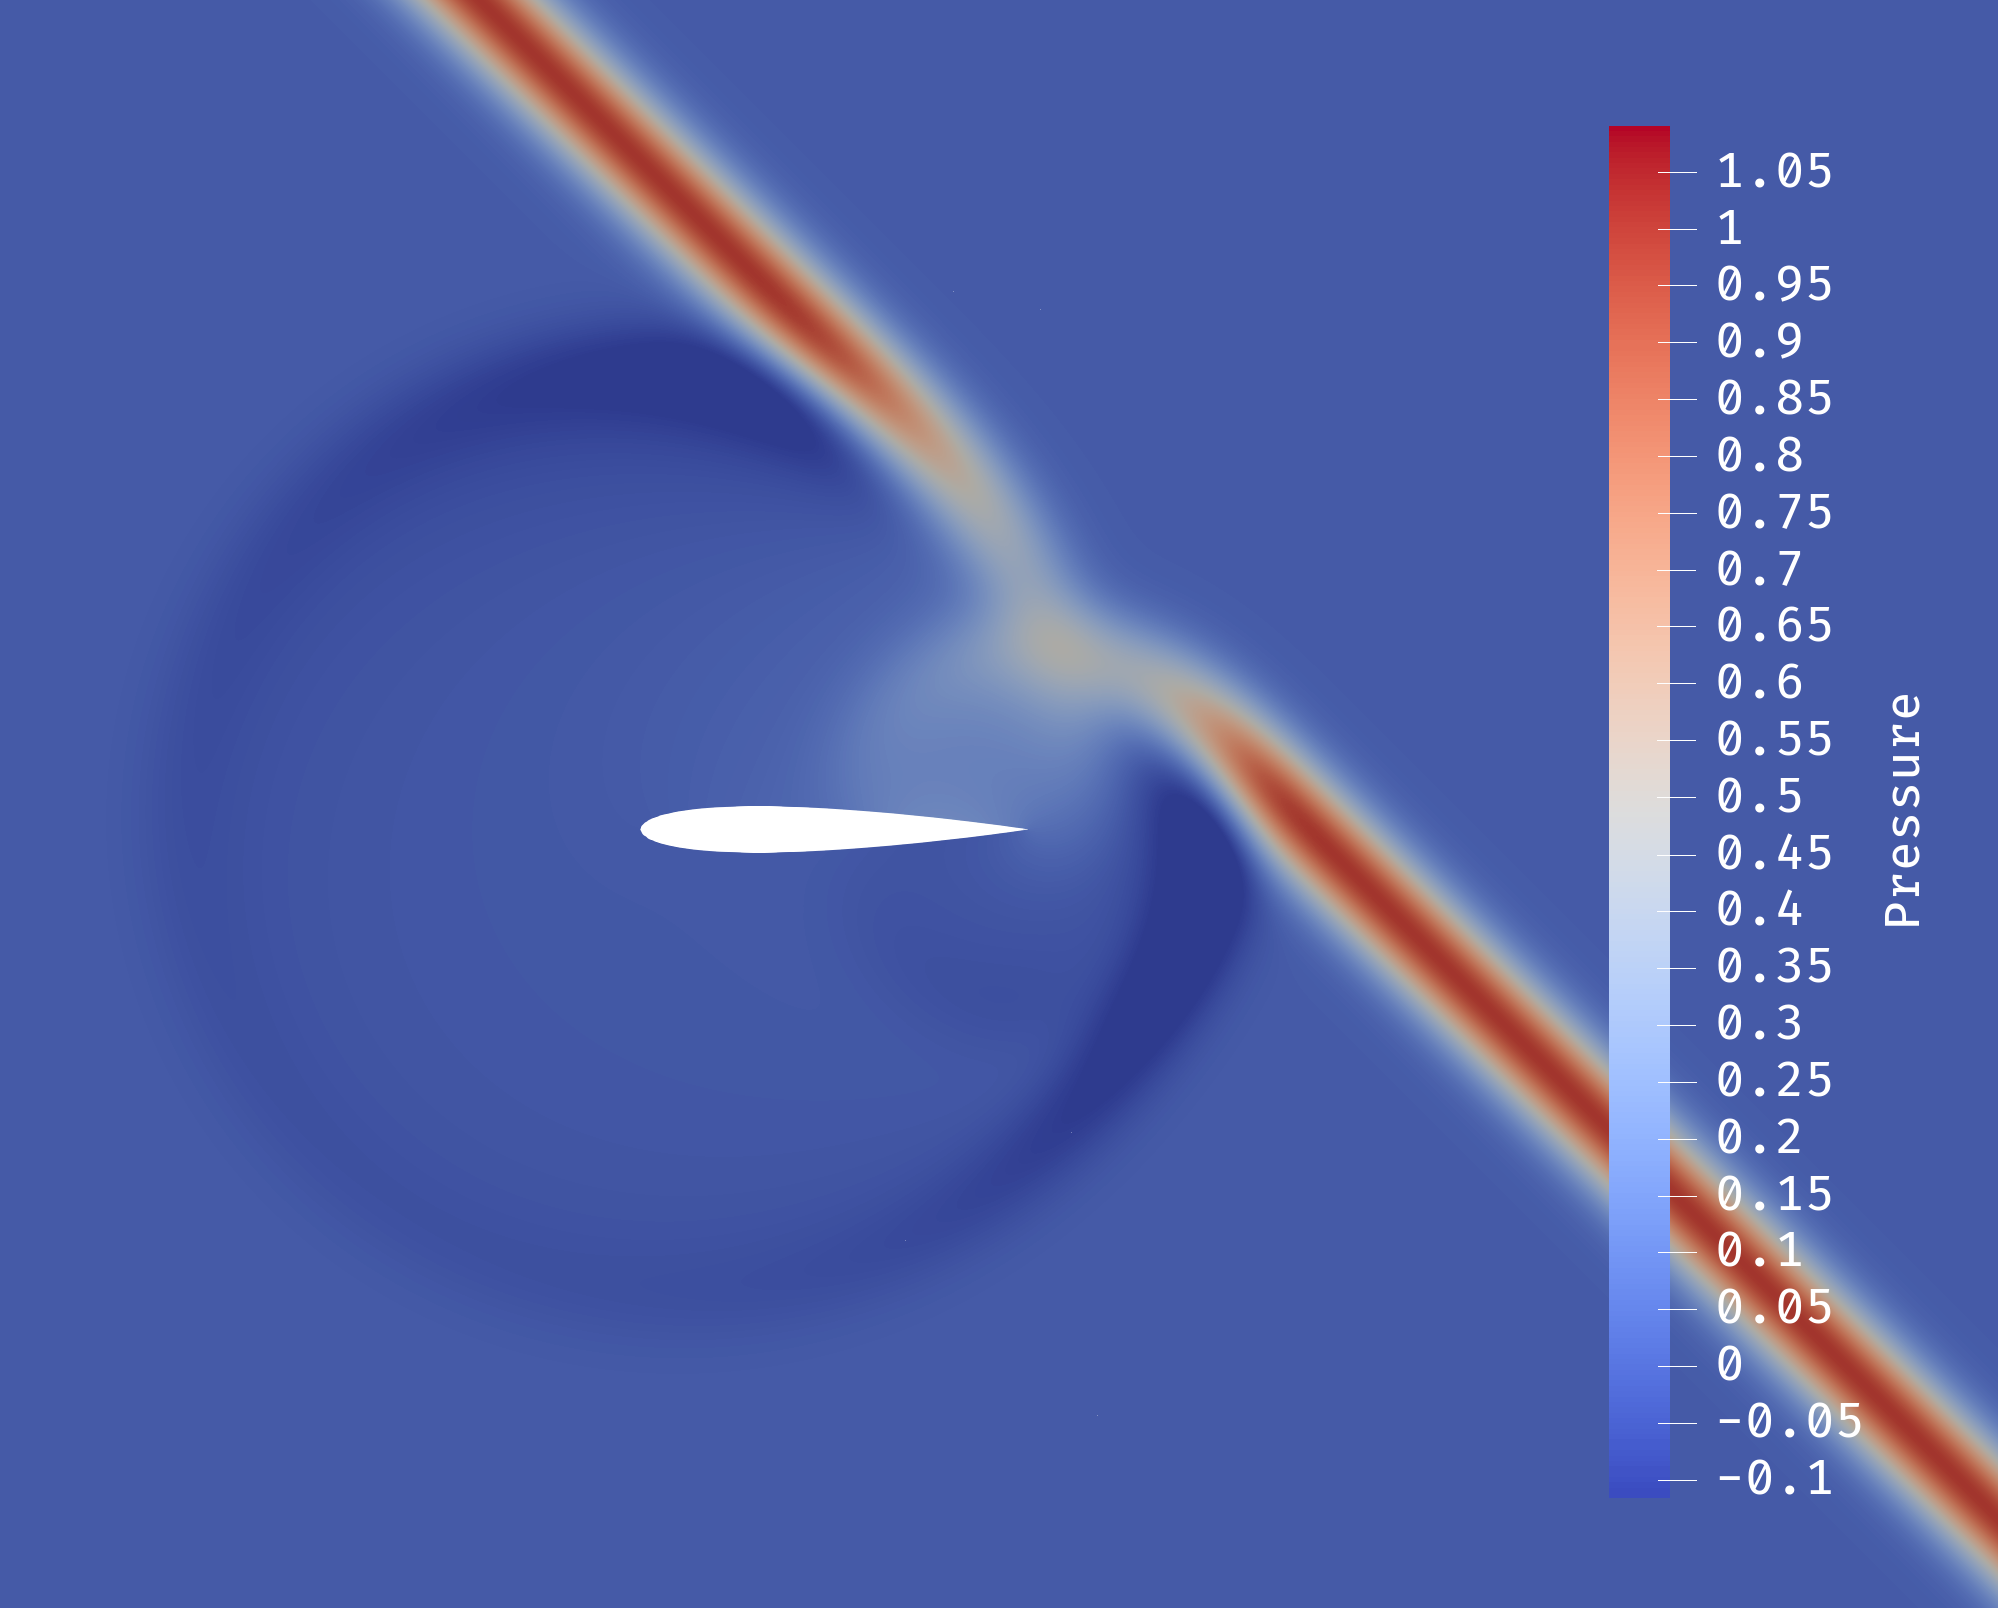
\includegraphics[width=0.48\textwidth]{Chapter_results/media/airfoil_pressure_near_t1_5}\label{fig:complex_mesh_solution_p}}
    \hfill
    \subfloat[Pressure \(\sigma \)]
    {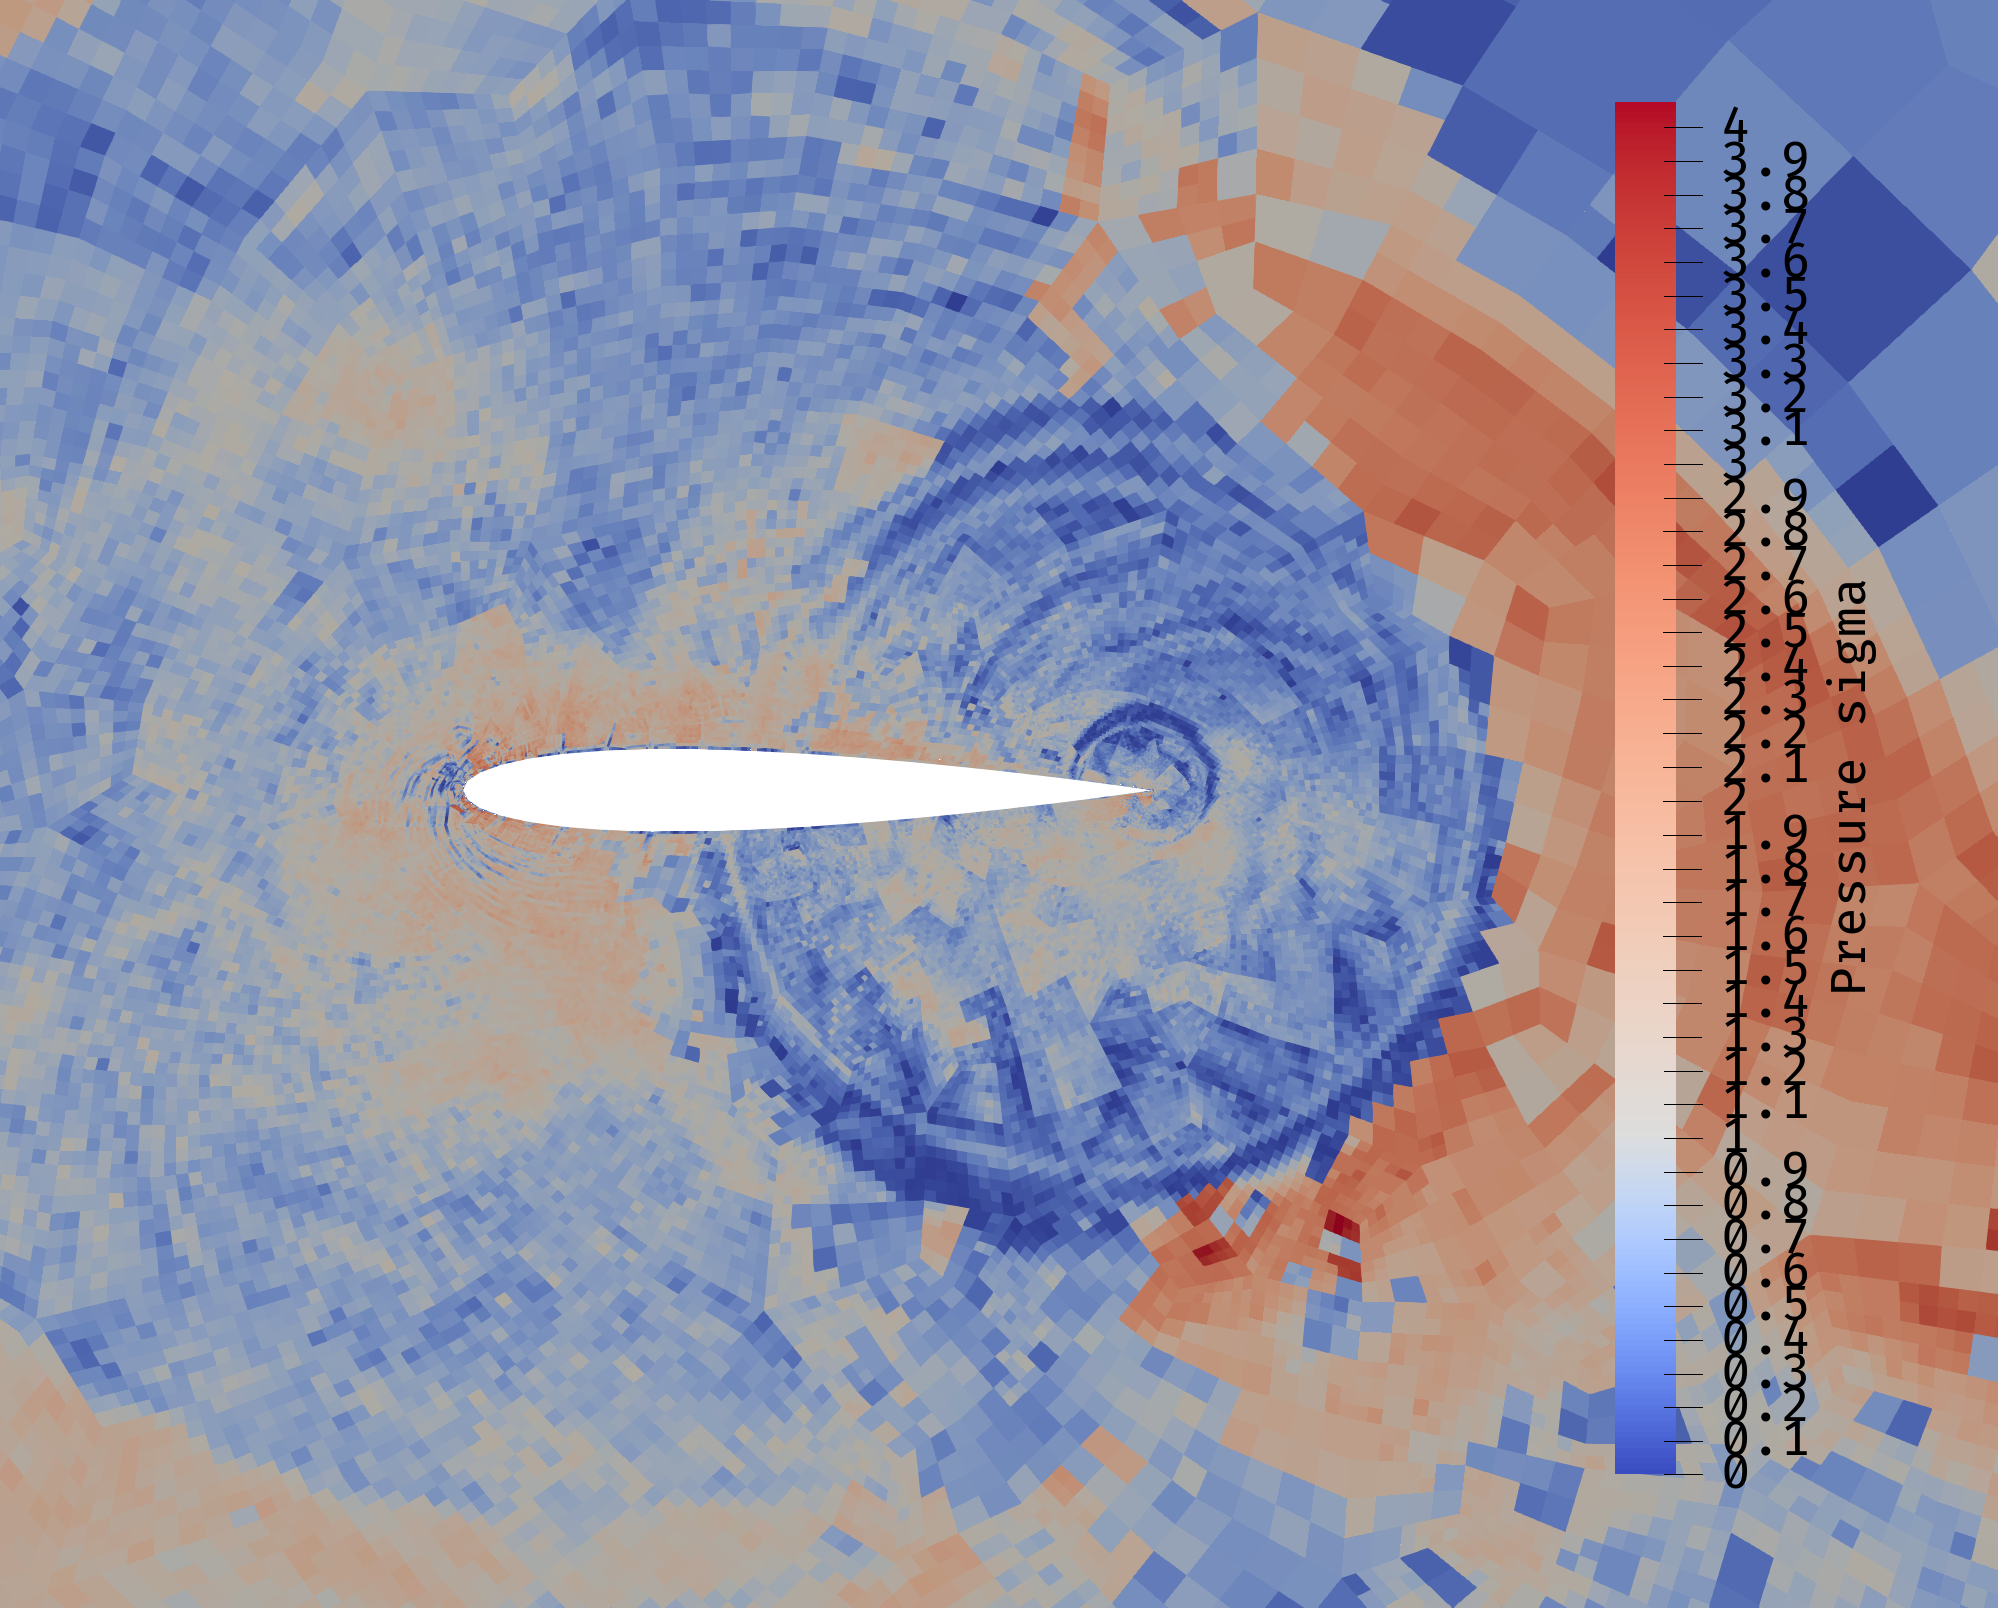
\includegraphics[width=0.48\textwidth]{Chapter_results/media/airfoil_pressure_sigma_near_t1_5}\label{fig:complex_mesh_solution_sigma}}
    
    \smallskip

    \subfloat[Split level]
    {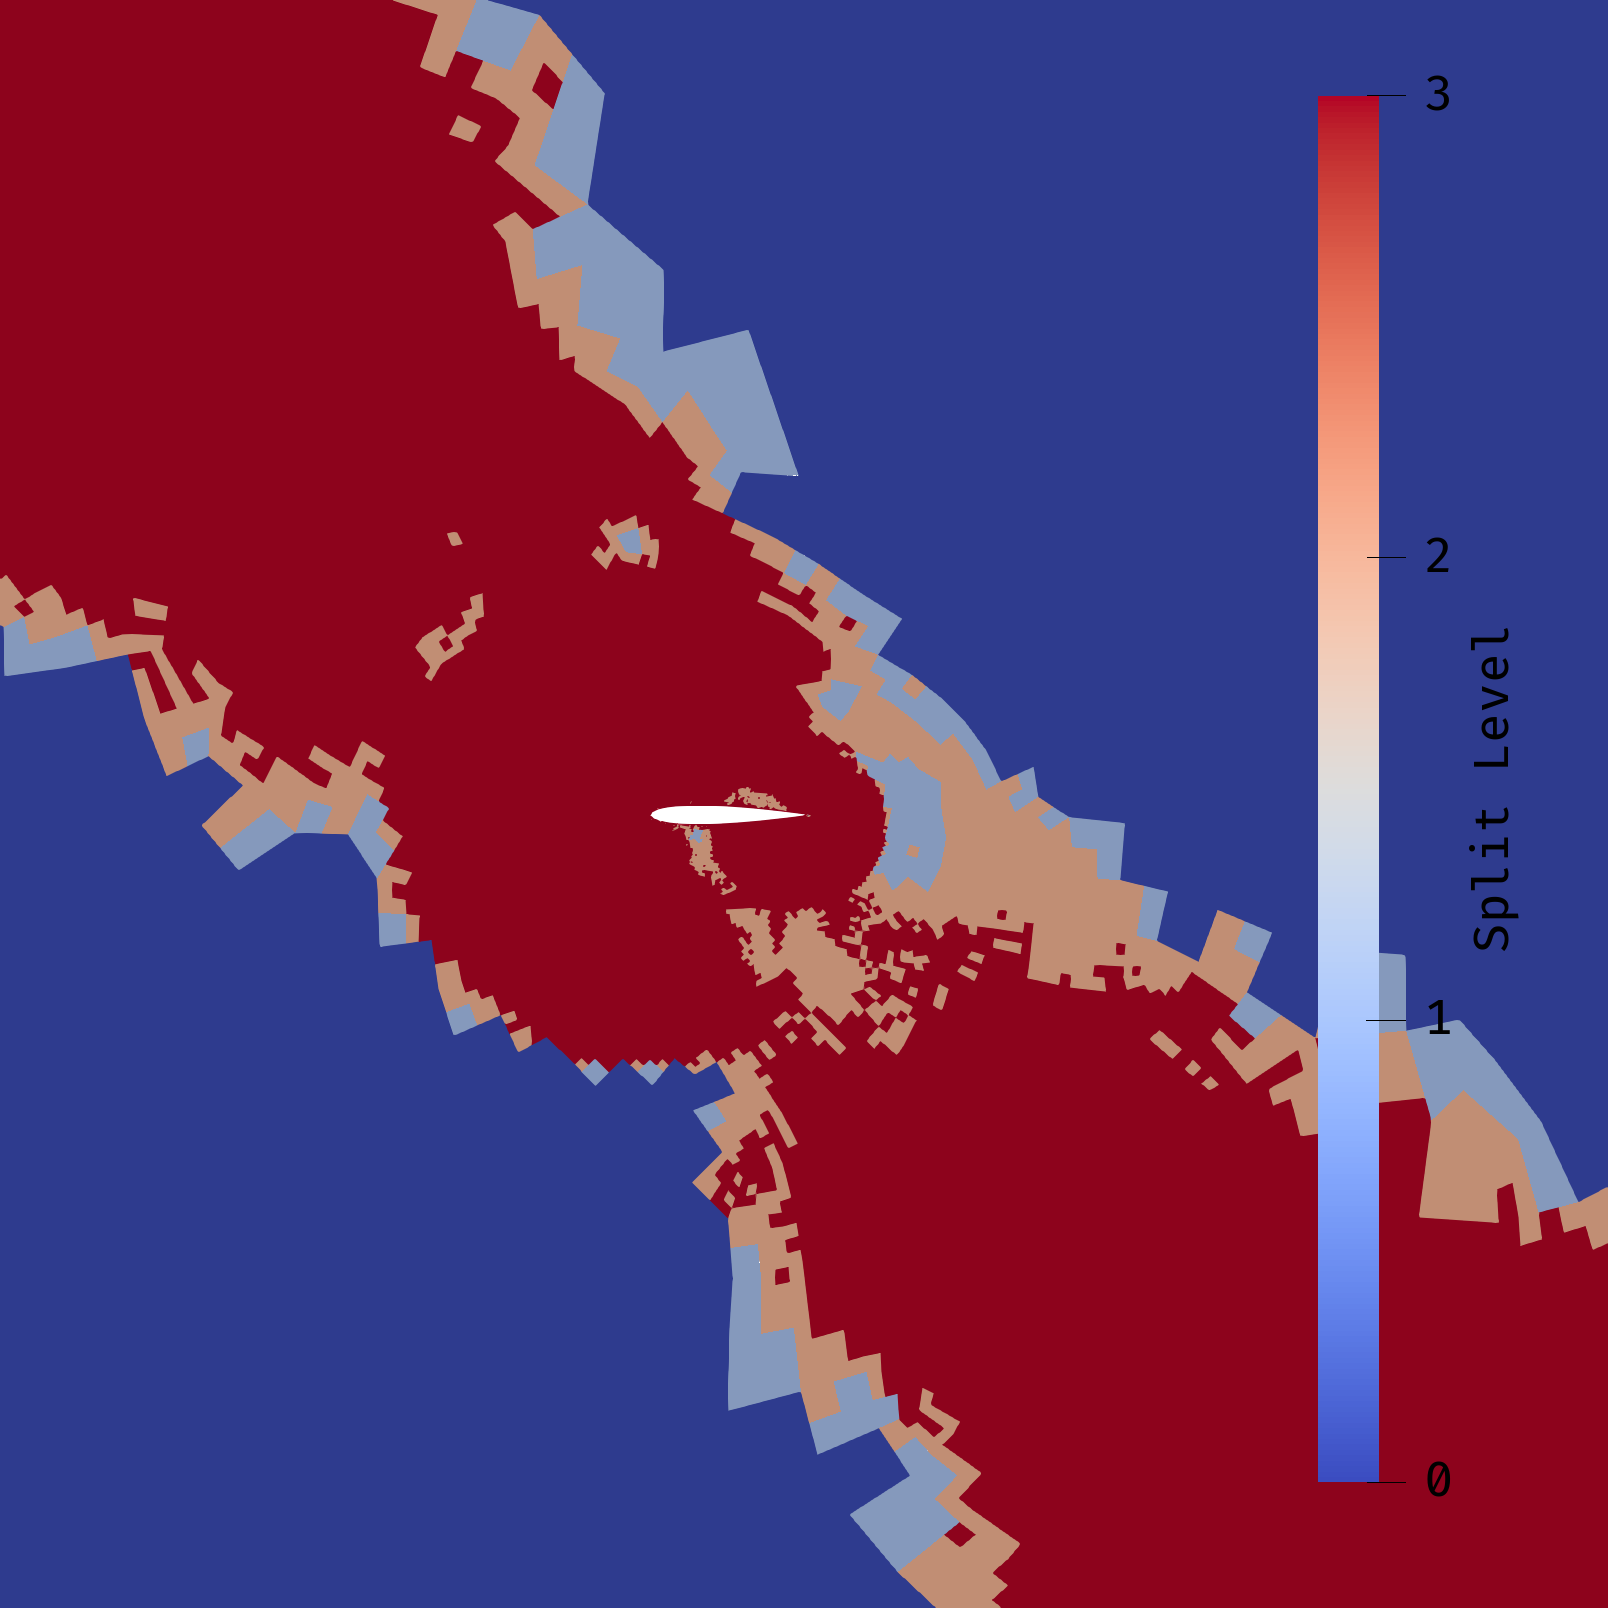
\includegraphics[width=0.48\textwidth]{Chapter_results/media/airfoil_split_level_t1_5}\label{fig:complex_mesh_split_level}}
    \hfill
    \subfloat[N]
    {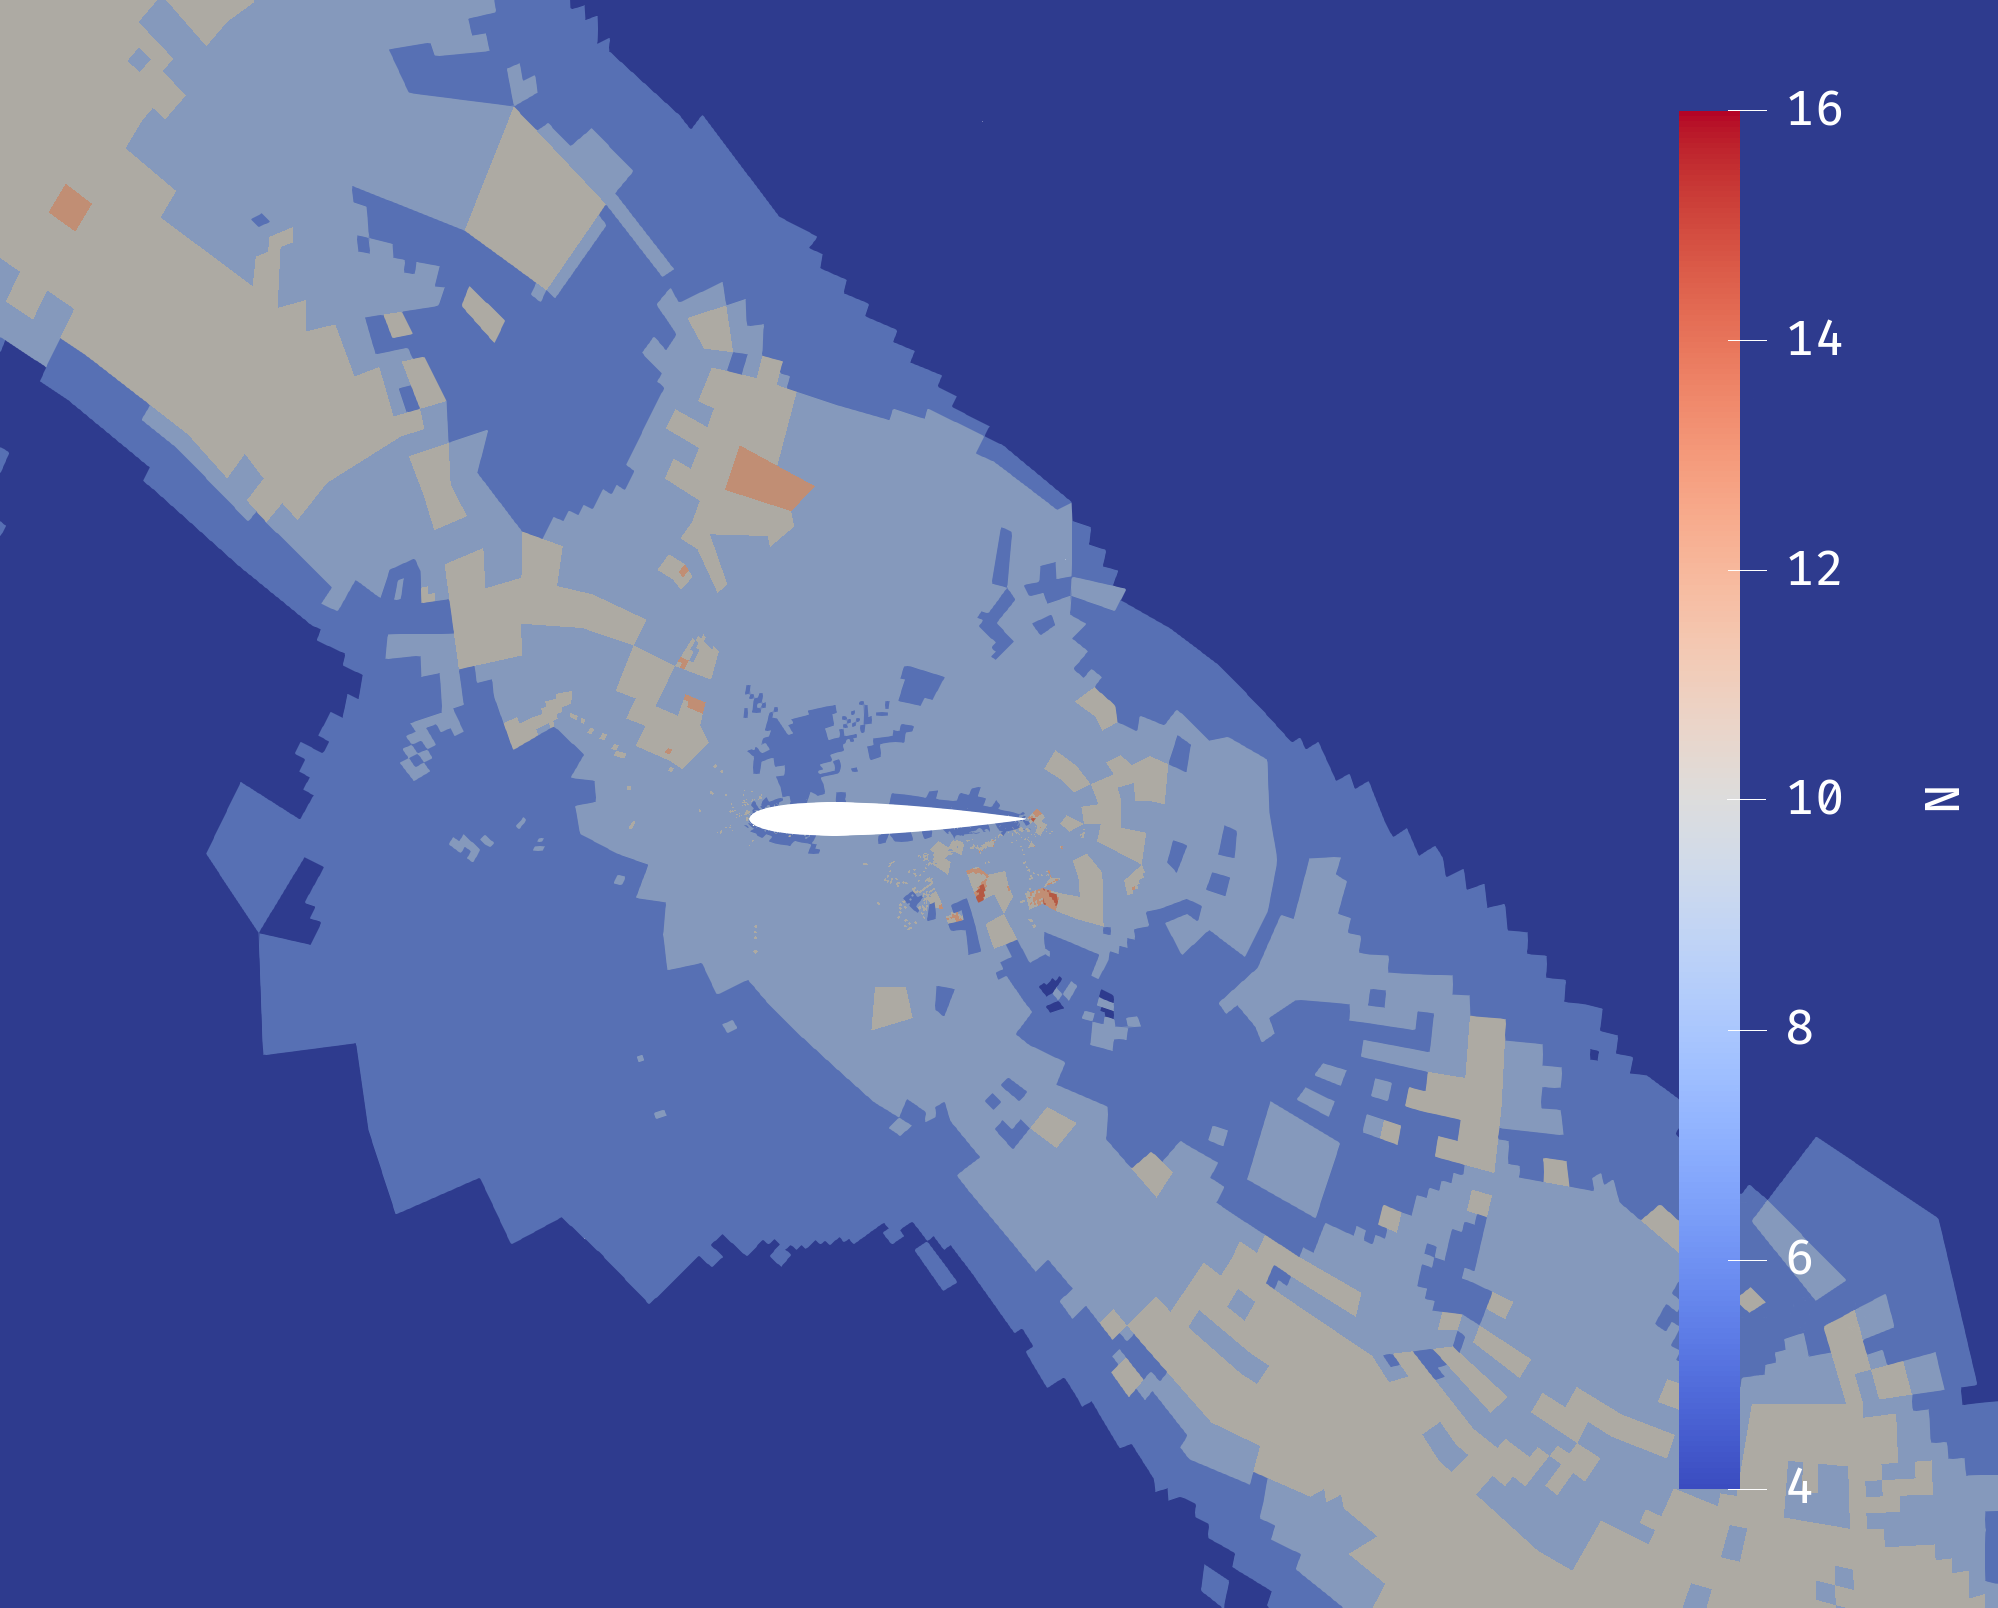
\includegraphics[width=0.48\textwidth]{Chapter_results/media/airfoil_N_t1_5_MOD}\label{fig:complex_mesh_N}}

    \caption{Complex mesh: A wave impinging on an airfoil at \(t = 1.5 s\). \(N_{initial} = 4\), \(K = 55680\), \(S = 3\), \(P = 4\) (a) Pressure (b) Pressure \(\sigma \), prescribing h-refinement or p-refinement (c) h-refinement, the split level denotes how many times elements have split (d) p-refinement, polynomial order \(N\)}\label{fig:complex_mesh_solution}
\end{figure}

Figure~\ref{fig:complex_mesh_solution} shows that the program has refined the mesh in more difficult
areas of the domain, such as along the linear wave, close to the airfoil, and inside the circular
wave. This is consistent with the fact that the interactions between the wave and the airfoil would
create steeper areas in the pressure distribution.

This also shows that the program is able to compute solutions on complex geometries, including
unstructured meshes where elements can be different from axis-aligned squares.

Figure~\ref{fig:complex_mesh_elements} shows how the elements are arranged among the four
\acrshortpl{acr:GPU}. Figure~\ref{fig:complex_mesh_index} shows the indices of the elements, or how
the elements are ordered along the pseudo-Hilbert curve. Figure~\ref{fig:complex_mesh_elements}
shows the elements' rank, or in which \acrshort{acr:GPU} they are stored.

\begin{figure}[H]
    \centering
    \subfloat[Element index]
    {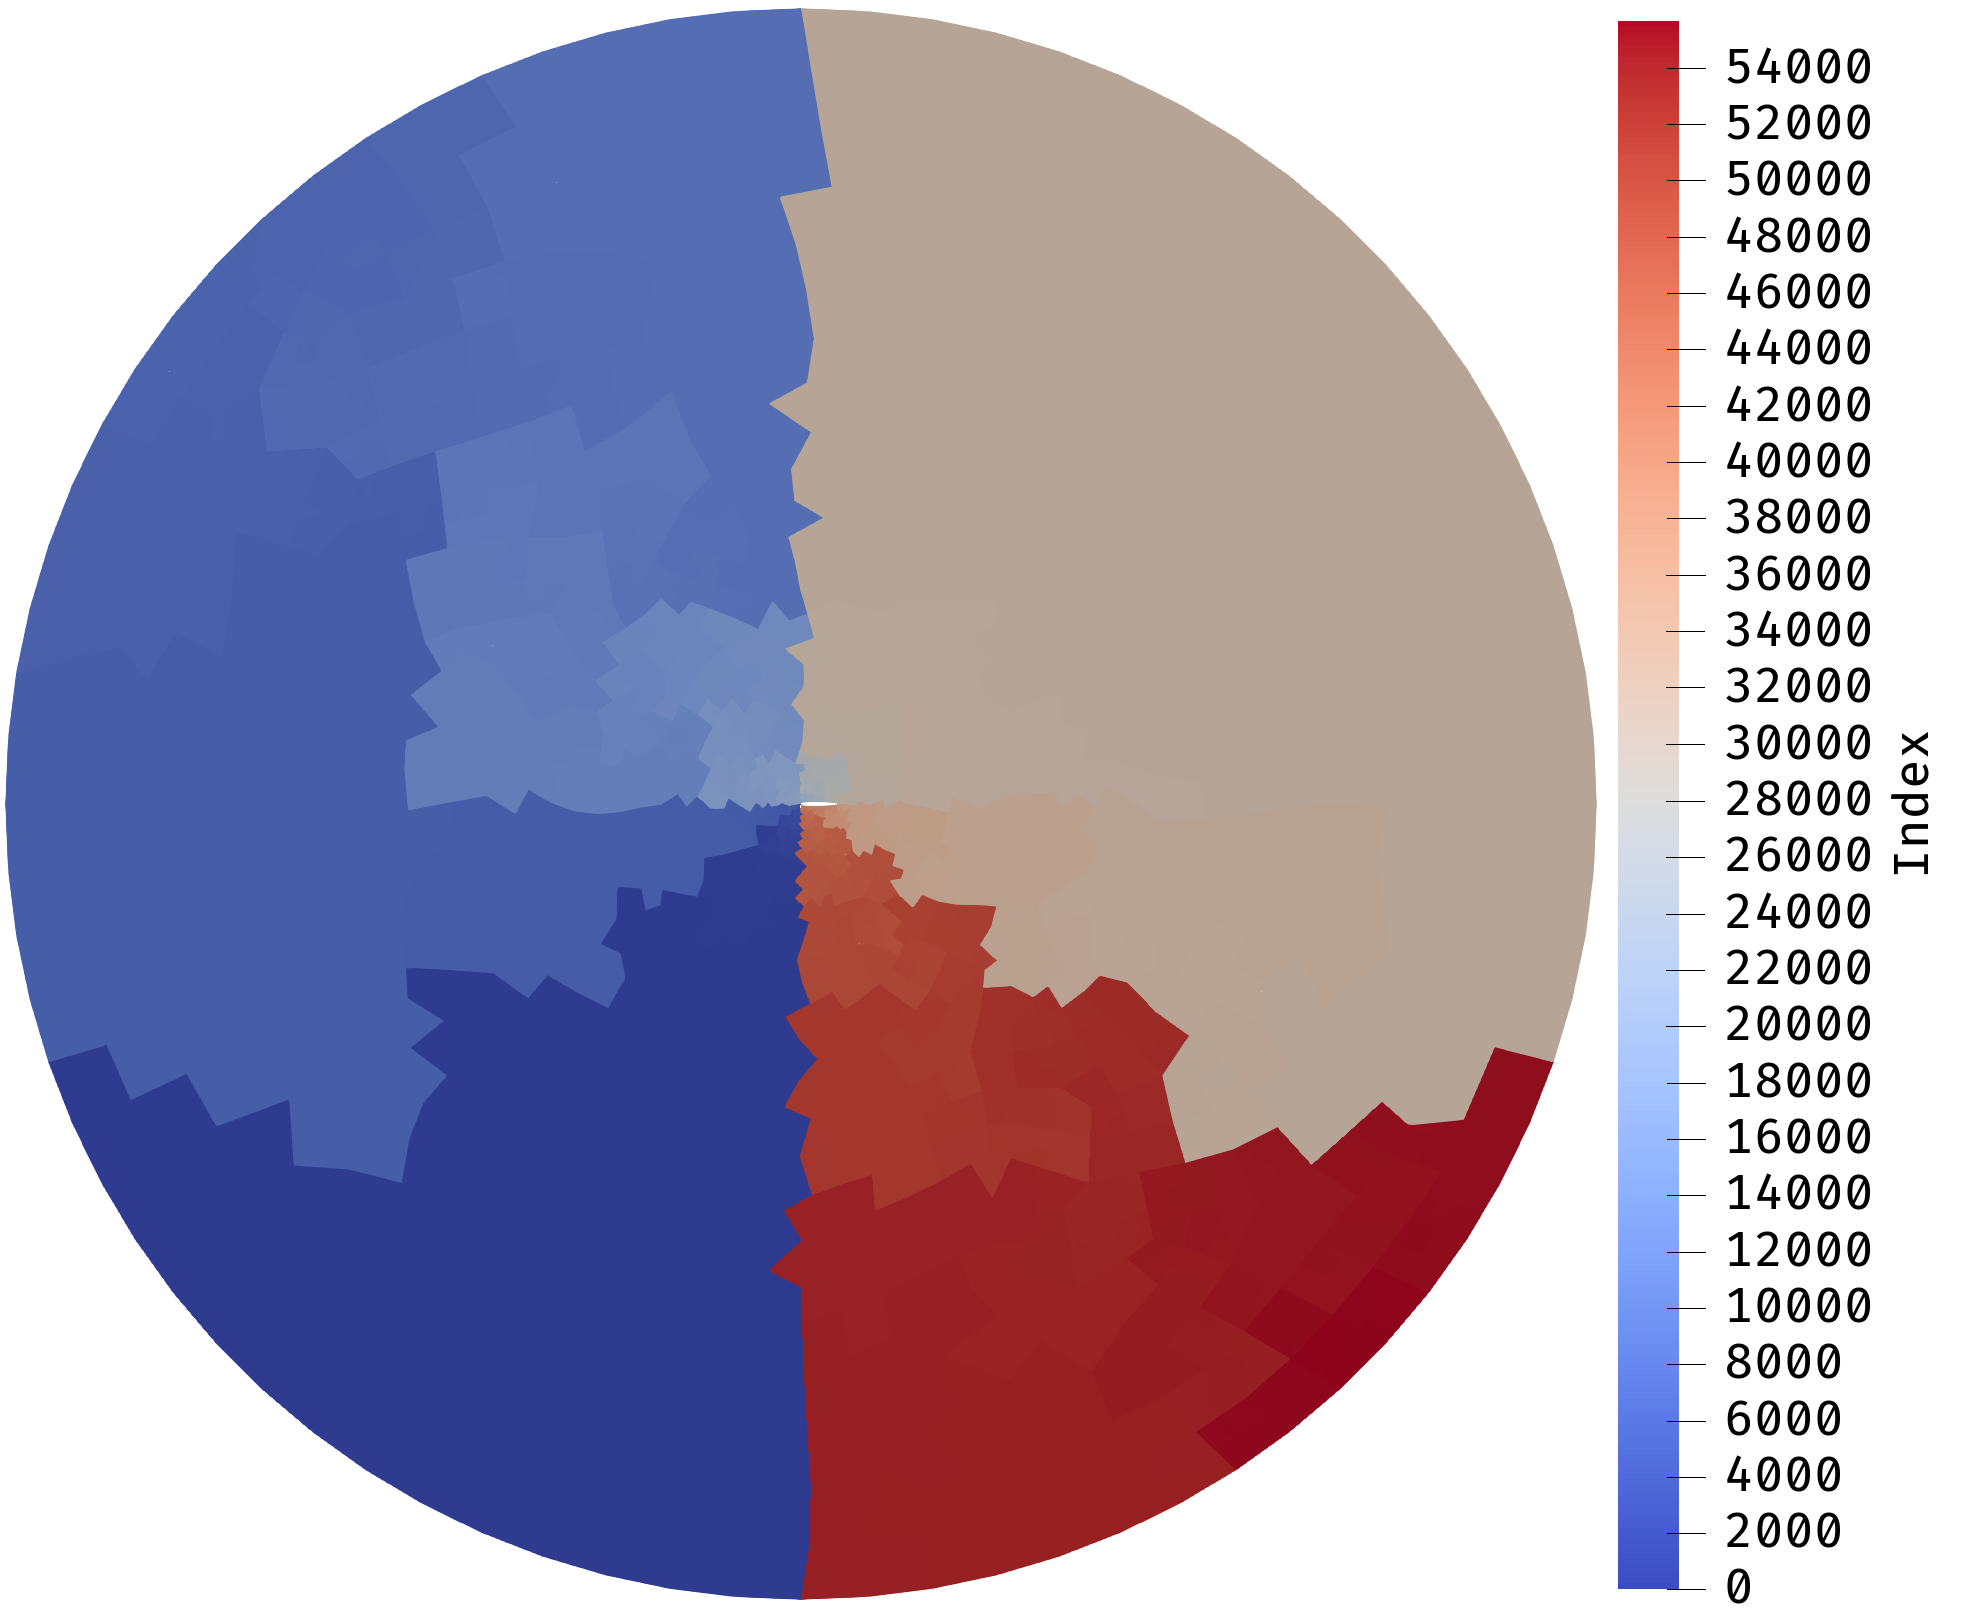
\includegraphics[width=0.48\textwidth]{Chapter_results/media/airfoil_index_t1_5_single}\label{fig:complex_mesh_index}}
    \hfill
    \subfloat[Rank]
    {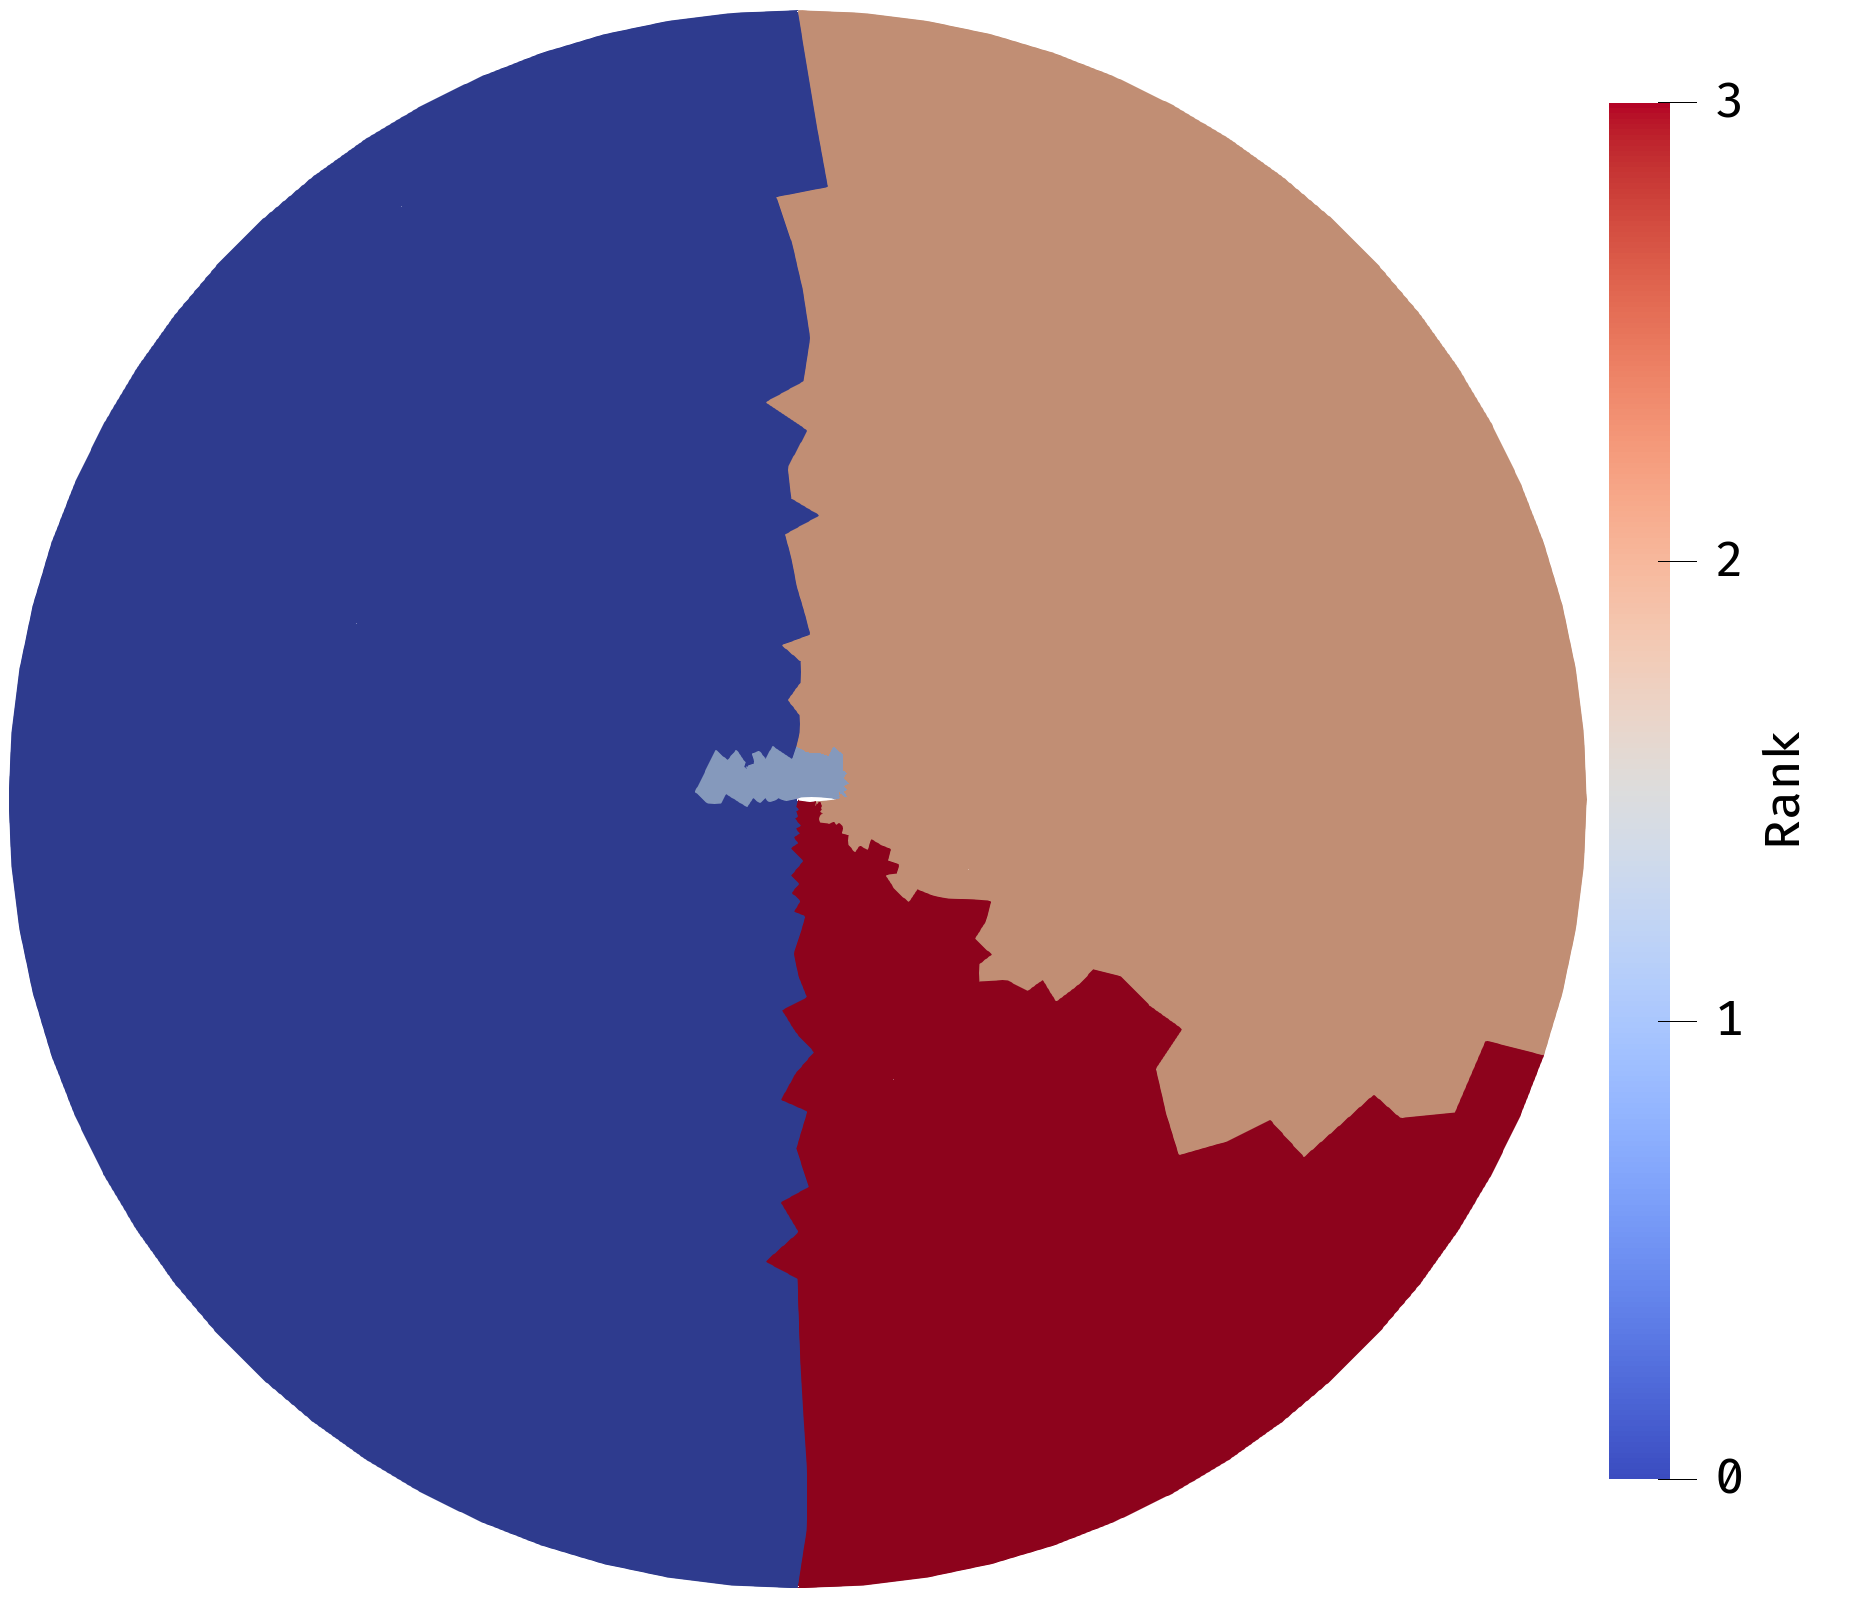
\includegraphics[width=0.48\textwidth]{Chapter_results/media/airfoil_rank_t1_5}\label{fig:complex_mesh_rank}}
    \caption{Element distribution: How elements are distributed between \acrshortpl{acr:GPU}. \(N_{initial} = 4\), \(K = 55680\), \(S = 3\), \(P = 4\) (a) Element indices, showing how they are ordered along the pseudo-Hilbert curve (b) Rank, showing which \acrshort{acr:GPU} contains which elements}\label{fig:complex_mesh_elements}
\end{figure}

On Figure~\ref{fig:complex_mesh_elements}, we can observe that the pseudo-Hilbert curve gives good
locality to the elements, there are few discontinuities between elements, and the surface area
between \acrshortpl{acr:GPU} is small. The elements are well divided between the
\acrshortpl{acr:GPU}, as the \acrshortpl{acr:GPU} in more heavily refined areas have a smaller
footprint in the domain.

\subsection{Profiling}\label{subsection:results:complex_meshes:profiling}

This complex case was also profiled in order to assess which parts of the program were more
computationally intensive. The simulation was run on four \acrshortpl{acr:GPU} up to \(t = 1 s\)
simulation time, refining every \(1000\) time steps and load balancing with a threshold of \(L =
1.1\). Table~\ref{table:profiling} shows the result of this profiling session. This is a report of
\acrshort{acr:GPU} time spent in the different kernels of the program. The report has a resolution
of \(0.1 \% \), therefore most smaller kernels are not shown here. This could artificially reduce
slightly the apparent time spent load balancing the mesh, as the load balancing module is made up of
many smaller kernels, which may not show up in the report. The numbers are the average time spent
between the four \acrshortpl{acr:GPU}. There may also be profiler overhead, especially when memory
is allocated and deallocated. This overhead could artificially inflate the time spent in memory
allocation heavy parts of the program like \acrshort{acr:AMR} and load balancing.

\begin{table}[H]
    \centering
    \begin{tabular}{ c c c c }
        Module & Time proportion (\%) & Algorithm & Time proportion (\%) \\
        \toprule
        \multirow{9}{*}{Solver} & \multirow{9}{*}{\(59.7\)} & compute\_derivative & \(26.68\) \\
                                                          & & project\_to\_elements & \(19.2\) \\
                                                          & & interpolate\_to\_edges & \(7.73\) \\
                                                          & & rk3\_step & \(3.75\) \\
                                                          & & project\_to\_faces & \(1.35\) \\
                                                          & & boundary\_conditions & \(0.37\) \\
                                                          & & compute\_fluxes & \(0.35\) \\
                                                          & & mpi\_interfaces & \(0.2\) \\
                                                          & & reduce\_delta\_t & \(<0.1\) \\
        \midrule
        \multirow{6}{*}{\Acrshort{acr:AMR}} & \multirow{6}{*}{\(38.5\)} & hp\_adapt & \(32.43\) \\
                                                                      & & split\_faces & \(2.63\) \\
                                                                      & & split\_mpi\_interfaces & \(2.55\) \\
                                                                      & & split\_boundaries & \(0.65\) \\
                                                                      & & p\_adapt & \(0.15\) \\
                                                                      & & estimate\_error & \(<0.1\) \\
        \midrule
        \multirow{3}{*}{Load balancing} & \multirow{3}{*}{\(1.4\)} & fill\_received\_elements & \(1.22\) \\
                                                                 & & create\_mpi\_boundaries & \(0.12\) \\
                                                                 & & create\_neighbours & \(<0.1\) \\
        \midrule
        \multirow{1}{*}{Other} & \multirow{1}{*}{\(0.7\)} & empty\_device\_vector & \(0.73\) \\
    \end{tabular}
    \caption{Program profiling: The relative \acrshort{acr:GPU} computation time spent in the three main modules, along with specific kernels and their relative \acrshort{acr:GPU} computation time.}\label{table:profiling}
\end{table}

This case ended up performing \(281078\) time steps, and took 5h04 to complete. The mesh was refined
281 times. These results show that the majority of the time is spent solving the problem and that
the time spent load balancing the mesh is small. This demonstrates very good performance of the
algorithm, with the only concerning result being the proportion of the computation time spent
refining the mesh. The high time spent in the \acrshort{acr:AMR} routine could be reduced by
refining the mesh less often, at the price of using a worse mesh for longer periods.
Section~\ref{section:conclusion:future_work} discusses a different approach to choose when to refine
the mesh which could improve these situations by only refining the mesh when a global target error
estimate is met.

    
    % conclusion
    \chapter{Conclusion}\label{chapter:conclusion}

\section{Summary}\label{section:conclusion:summary}

In this work, we presented a \acrshort{acr:GPU}-based wave equation solver using the
\acrlong{acr:DG-SEM}, as well as \acrlong{acr:AMR} and dynamic load balancing. The main
contributions of this work are: showing that \acrshort{acr:AMR} and load balancing on
\acrshortpl{acr:GPU} is possible and beneficial to solution quality and performance, showing that
significant performance can be gained by performing computations using \acrshortpl{acr:GPU}, and
showing that \acrshortpl{acr:GPU} accelerate spectral methods significantly.

The goal of using \acrshortpl{acr:GPU} to perform these computations was to increase the available
computing power, as spectral methods are notoriously expensive to compute. Spectral methods are
useful when highly accurate solutions of complex flows are needed.
Section~\ref{section:results:scaling_tests} shows that a baseline case without \acrshort{acr:AMR}
can be computed on a \acrshort{acr:HPC} platform up to three times faster using \acrshortpl{acr:GPU}
when they are sufficiently loaded. The program has also been shown to scale well up to \(64\)
\acrshortpl{acr:GPU}. Chapter~\ref{chapter:graphics_processing_units} discusses the architectural
decisions taken to use the massively parallel \acrshort{acr:GPU} architecture. One such decision is
to implement a data structure such that only high-level objects such as elements and faces are
stored in flat arrays that can be transferred from the \acrshort{acr:GPU} to the \acrshort{acr:CPU}.
The data arrays within those objects are instead allocated directly by the \acrshort{acr:GPU} in
\acrshort{acr:GPU} code, and stored in dynamic memory. This allows for a more flexible data
structure, where the \acrshort{acr:GPU} itself can perform some of the dynamic mesh changes
necessary for \acrshort{acr:AMR} and load balancing, and reduces the overhead of moving objects
around because the bulk of the data is stored outside of the objects themselves.

Some problems have localised areas where more precision is needed, such as shocks and boundary
layers. Even with the increased processing power of \acrshortpl{acr:GPU}, uniformly refining a mesh
to the level needed by those areas makes the computing time increase to the point where it is not
economic to solve these problems. We use \acrlong{acr:AMR} to assess which parts of the problem have
a higher level of estimated error and to refine them, all while the program is running.
Section~\ref{section:results:adaptivity_performance} shows that a case with \acrshort{acr:AMR} can
be more than \(67 \times \) faster to execute than the same case initially uniformly refined to the
same level as the \acrshort{acr:AMR} case. When compared to another case initially uniformly refined
to the point that it reaches a similar maximum error to the \acrshort{acr:AMR} case, the
\acrshort{acr:AMR} case is still generally faster. This is an excellent result, given that
\acrshortpl{acr:GPU} are not tailored to these kinds of dynamically changing computations. 

The \acrshort{acr:AMR} process itself does not match well with the \acrshort{acr:GPU} architecture,
as it reallocates and moves large amounts of memory, and is fundamentally sequential. Since each
\acrshort{acr:GPU} is paired with a single \acrshort{acr:CPU} and is vastly faster, we want to
execute as much as possible of the process in parallel on the \acrshort{acr:GPU}. We devised an
algorithm to perform \acrshort{acr:AMR} in parallel, described in
Chapter~\ref{chapter:adaptive_mesh_refinement}, offloading most of the computation to the
\acrshort{acr:GPU}. Moving elements, h-refining, p-refining and the renumbering that comes with the
process are all executed on the \acrshort{acr:GPU}. The only significant parts executed on the
\acrshort{acr:CPU} are the allocation of the resized high-level arrays and the computing of offset
arrays, so that the different \acrshort{acr:GPU} threads can operate in parallel without race
conditions. Despite this, \acrshort{acr:AMR} can be a costly process on \acrshortpl{acr:GPU}, for
example in Subsection~\ref{subsection:results:complex_meshes:profiling} where it makes up a
significant portion of the total runtime.

We also implement a mesh pre-condition algorithm, described in
Section~\ref{section:adaptive_mesh_refinement:pre_conditioning}, to refine the mesh before the
computation up to a point where initial conditions are well resolved.
Section~\ref{section:results:adaptivity_performance} shows that performing a few pre-condition steps
can significantly increase the solution quality when the starting mesh is very coarse. Combined with
\acrshort{acr:AMR}, this means that meshes do not need to be very tailored to problems. A uniform
coarse mesh can be used, and the pre-condition will refine the mesh to capture initial conditions
correctly, while \acrshort{acr:AMR} refines the mesh as the solution is computed to capture the
important areas of the flow.

To combat the load imbalance that can arise when the problem is solved in parallel using multiple
\acrshortpl{acr:GPU}, we implemented a dynamic load balancing algorithm. The algorithm uses the
Hilbert curve, a \acrlong{acr:SFC} that has good locality. This is especially important when using
\acrshortpl{acr:GPU} because data transfers between \acrshortpl{acr:GPU} are more expensive,
therefore we want to reduce the size of the boundaries between mesh blocks as much as possible.
Section~\ref{section:results:load_balancing_performance} shows that dynamic load balancing
significantly increases performance when there is load imbalance. The performance increase scales
well with load imbalance, meaning that dynamic load balancing should improve the performance no
matter how much load imbalance is present. By judiciously choosing when we load balance, as
explained in Section~\ref{section:load_balancing:criteria}, the computing time spent in the load
balancing algorithm can be very low, as reported in
Subsection~\ref{subsection:results:complex_meshes:profiling}. 

Load balancing is hampered  by the same limitations as \acrshort{acr:AMR}, namely that it is not
particularly well suited for the \acrshort{acr:GPU} architecture, and we want to execute as much of
it as possible on the \acrshort{acr:GPU}. \Acrshortpl{acr:GPU} have less memory than
\acrshortpl{acr:CPU}, therefore we want each worker \acrshort{acr:GPU} to only have knowledge about
the mesh block it is assigned in order to reduce its memory footprint. This complicates load
balancing, as it is harder to reconstruct the mesh once elements are exchanged. Because of this, the
load balancing algorithm is made up of several smaller dependent functions, in order to catch every
possible edge case. Most of those functions execute on the \acrshort{acr:GPU}, including the
generation of the Hilbert curve ordering of the elements. This algorithm has a good performance,
despite performing many data transfers between \acrshortpl{acr:GPU} and reallocating a lot of
memory. Chapter~\ref{chapter:load_balancing} details how the algorithm is designed, and what
strategies were used to make it perform well on \acrshortpl{acr:GPU}.

Another significant conclusion is that \acrshortpl{acr:GPU} are particularly well suited to the
spectral methods, specifically. As described in Chapter~\ref{chapter:spectral_element_method}, the
number of operations to perform every time steps scales with \({\left( N + 1 \right)}^2\), where
\(N\) is the polynomial order of an element. This indicates that the computational complexity should
scale with \({\left( N + 1 \right)}^2\). However, as reported in
Subsection~\ref{subsection:results:load_balancing_performance:polynomial_order}, it seems that
increasing the polynomial order of elements increases the density of computations, which lends
itself to better performance. The computation time relative to \(N\) seems closer to a linear
relation than an exponential one. This means that using higher order elements, with the benefit of
higher accuracy, is more attractive on \acrshortpl{acr:GPU} than on traditional platforms. It also
points to the fact that spectral methods in general could have an increased speedup when using
\acrshortpl{acr:GPU} compared to other methods.

\section{Concluding Remarks}\label{section:conclusion:remarks}

The \acrshort{acr:AMR} and load balancing algorithms destined for \acrshortpl{acr:GPU} are very
different from those destined for \acrshortpl{acr:CPU} only. Many different strategies must be used,
such as optimising each and every part of the algorithm in terms of what can be executed in parallel
on shared memory and what cannot. These parts should be executed on the \acrshort{acr:GPU} in order
to improve performance and avoid unnecessary copies from the \acrshort{acr:GPU} to the
\acrshort{acr:CPU}. Once these parallel parts have been identified, they must be modified until they
operate on a single object type. For example, a kernel that is parallelised over elements and moves
elements to a new index can modify the elements, arrays that are indexed per element, but it cannot
modify faces. This is because multiple elements can link to the same face. If for example that
kernel would update the element indices in the faces, a race condition would occur and the results
would not be correct. In this case, the faces should update their element indices in another kernel,
that parallelises over faces. There are many such issues that do not impact sequential code but
start appearing when a few thousand threads execute in parallel.

Another noteworthy difference about \acrshort{acr:GPU} computing is that surprising things can have
an impact on performance. One example is increasing the thread block size in
Subsection~\ref{subsection:results:scaling_tests:strong}. Increasing the block size should improve
performance by reducing the number of instructions to dispatch. This is because there is a lot of
divergence in the code, and with an increased block size more threads will be waiting for divergents
threads. It is important to profile the code and look at which parts are taking up more time than
they should. Sometimes some problematic functions can be made much faster, such as the error
estimation routine that went from taking up \(15 \% \) of the total execution time to \(0.1 \% \) by
precomputing a set of values.

The \acrshortpl{acr:GPU} need to be saturated with work in order to have good performance. This can
lead to peculiar situations like those in Subsection~\ref{subsection:results:scaling_tests:strong},
where the relation between number of elements in a \acrshort{acr:GPU} and the computation time is
not linear. Under a certain workload, the cores of a \acrshort{acr:GPU} do not all have work to
perform, and the \acrshort{acr:GPU} is partly idle. On the other hand, if there is too much work in
a \acrshort{acr:GPU} its memory may fill up, or the constant cache swapping from each core working
on different elements successively may degrade performance. There is an ideal amount of work per
\acrshort{acr:GPU} to be found, depending on the problem.

Thread divergence can also cause surprising results, such as a single if/else statement reducing the
performance of a function by half. For example, the projection from faces to elements has four
different paths, depending on if the face is forward or backward compared to the element, and if it
is conforming or not. Since threads execute in groups of 32, threads that do not take a particular
branch are stopped while the threads that took that branch execute, and then the next branch is
evaluated. For our projection, if it happens that there are threads that take each of the four
branches in a group, each of the branches will be executed one after the other with different
threads inactive, taking up four times as much time as it should. This is a significant difference
when programming for \acrshortpl{acr:GPU}: branching must be minimised as much as possible.

It is also difficult to program dynamic meshes on the \acrshort{acr:GPU}. The fact that neither the
\acrshort{acr:CPU} or \acrshort{acr:GPU} have the complete picture, and that all data has to be
transferred from one to the other complicates some of the algorithms. Load balancing in particular
required the most changes compared to a sequential \acrshort{acr:CPU} algorithm. In that algorithm,
there are many dependencies between the different parts, which must be computed in a specific order.
It is possible that it would be easier to re-create the mesh once elements have been exchanged, and
rebuild all the connectivity from scratch. That approach was not chosen; instead the mesh is
modified to remove unneeded parts and add new parts. Seeing that modifying the mesh with limited
information is very difficult and error-prone, it is hard at this stage to say which approach is
best.

\section{Future Work}\label{section:conclusion:future_work}

\subsection{GPU Computing}\label{subsection:conclusion:future_work:gpu}

There is still a lot of work to be done in order to better match the \acrshort{acr:GPU} architecture
to the different modules of the program. For one, there is a lot of divergence in the code, due to
\acrshort{acr:AMR} creating elements with different polynomial orders and non-conforming interfaces
among other things. An avenue for future work would be to try to reduce divergence as much as
possible. For example, sorting the faces by type and storing them in different arrays would allow
different kernels to be launched for each type of face. In that case, each \acrshort{acr:GPU} thread
in a kernel would execute the same instructions and there would be no divergence. Similarly,
refining elements per block would alleviate divergence, in that the elements assigned to a block of
threads are always kept the same and there is no divergence.

Another approach would be to decompose the objects, like faces and elements, to a separate array for
each member. This means changing from an ``array of structures'' to a ``structure of arrays'' data
structure. This could help alleviate cache pressure, since \acrshortpl{acr:GPU} have smaller caches
than \acrshortpl{acr:CPU}. This helps by reducing the amount of data that has to be loaded in cache
since only the data members used can be loaded instead of whole objects. This could improve
performance, especially when the \acrshort{acr:GPU} is very loaded.

There is also always work to be done by profiling the code and examining which parts of the code
take up more execution time than they should, or are not optimal. Many tools exist to profile
\acrshort{acr:CUDA} code. Two profilers were used to summarily examine the code for this work. The
first is an overall profiler, the result of which is shown in
Subsection~\ref{subsection:results:complex_meshes:profiling}. The other is a profiler for single
kernels, which was used to improve the error estimation kernel. These tools give a lot of
information, such as latency statistics, data dependencies, and optimal occupancy of the
\acrshort{acr:GPU}.

There is no reason to use only \acrshortpl{acr:CPU} or only \acrshortpl{acr:GPU}. A future path to
explore is to make a hybrid solver. If the program was modified to enable using both
\acrshort{acr:CPU} and \acrshort{acr:GPU} workers together, it would be possible to use the complete
processing power of computers. Since \acrshortpl{acr:CPU} and \acrshortpl{acr:GPU} have very
different computing powers and capacities, this would make load balancing more difficult as elements
would need to be split unequally between the workers. Since we implemented a \acrshort{acr:CPU}
version of the program as a comparison, and both versions have the same interface between workers,
it was possible to create a crude hybrid version to assess its potential. This tentative hybrid
version is presented in Appendix~\ref{chapter:hybrid_solver}.

Finally, another area of work would be to add more fine-grained parallelism. As it stands, every
process communicates with others via \acrshort{acr:MPI}. This happens regardless of if
the other process is on the same machine or not. Workers on the same machine could access the same
memory, and even transfer data between \acrshortpl{acr:GPU} directly if they are connected together.
We could use multithreading in addition to multiprocessing, where there is one process per machine
and all workers on a machine execute via threads. This would completely remove necessary transfers
between workers on the same machine, as they could all access the same data. This would also reduce
the number of \acrshort{acr:MPI} transfers needed, as only one process per machine would need to
communicate.

\subsection{DG-SEM}\label{subsection:conclusion:future_work:dg_sem}

In this work, we solved the wave equation. We use this simple equation in order to show the program
works, but it is not very useful in itself. A possible avenue would be to upgrade the solver to
solve a more interesting and complex equation. For example, solving the full Navier-Stokes equations
would make the program useful for solving real-world problems.

Another possible improvement is using different shapes other than quadrilaterals, ideally within the
same mesh. Many meshes use triangles, and some unstructured meshes use a mix of quadrilaterals and
triangles. Some meshes even use elements with an arbitrary number of sides. Supporting these element
types would make the program more general and able to work with more off-the-shelf meshes. This
would mean changing the structure of the program to be generic over element types.

Speaking of elements, we often want to model curved surfaces, such as the airfoil from
Subsection~\ref{section:results:complex_meshes}. In order to model curved surfaces with
straight-edged elements, the elements need to be very small, and only approximate such surfaces.
Implementing curved elements would help model these geometries better. An added advantage of curved
elements is the possibility of smoothing the transition between very skewed elements, which becomes
a problem with more complex equations.

Finally, it would be very interesting to transform the program from a 2D solver to a 3D solver. Many
interesting problems appear only in 3D, and more complex geometries can be modeled. Also, 3D
problems are an order of magnitude more computationally intensive to solve. These problems would
benefit even more from the computational power of \acrshortpl{acr:GPU} and would have no problem
saturating them with work thanks to the increased complexity. With another dimension to fill, the
number of elements that is possible to put in each dimension is reduced. This means that
\acrshort{acr:AMR} is even more crucial in 3D, as computational resources are limited. The
computational complexity increases from \({\left( N + 1 \right)}^2\) to \({\left( N + 1 \right)}^3\)
in 3D, where \(N\) is the polynomial order. The scaling shown in
Subsection~\ref{subsection:results:load_balancing_performance:polynomial_order} could help with that
increased complexity.

\subsection{AMR}\label{subsection:conclusion:future_work:amr}

There is also work to do to improve \acrlong{acr:AMR}. Firstly, it takes up a large proportion of
the total computation time. Maybe being more judicious about when we refine could alleviate this
problem. There could be a global target error estimate below which the \acrshort{acr:AMR} routine is
not launched, similar to the load balancing threshold described in
Section~\ref{section:load_balancing:criteria}. Care should be taken to not compromise efficiency by
refining more often than necessary. It may also be possible to refine only some parts of the mesh,
and avoid moving and reallocating the whole mesh.

As it stands now, we do not perform mesh coarsening in this work. This is an important avenue to
explore, as it saves even more resources than refinement alone. In many cases, such as the one shown
in Section~\ref{section:results:test_case}, the areas that need refinement are not static in space.
In that example, a wave goes through the domain diagonally. As it advances, the mesh is refined to
better capture the wave. In its wake are left many very refined elements that do not contribute to
the solution anymore, as the wave is not present in those areas. These elements take up computation
power for no benefit. Mesh coarsening would do the inverse of h-refinement and p-refinement, and
either lower the polynomial order of elements or merge elements together. This would be a
significant challenge to add to the program because of its flat arrays data structure. Many
\acrshort{acr:AMR} programs store their elements in a tree data structure in order to keep track of
which elements are the children of which and to be able to re-form elements that have split. In our
data structure, elements resulting of h-refinement are just regular elements like any other, and
have no knowledge of their previous topology. Coarsening would imply searching through nearby
elements for other elements to be coarsened that can form a quadrilateral together. This is
difficult, but brings the interesting ability of re-forming elements that did not exist previously.

\subsection{Dynamic Load Balancing}\label{subsection:conclusion:future_work:load_balancing}

The implementation of dynamic load balancing we present operates on the assumption that all elements
have the same weight and are all equally as expensive to compute. With \acrshort{acr:AMR}, all
elements can have a different polynomial order. As shown in
Subsection~\ref{subsection:results:load_balancing_performance:polynomial_order}, the polynomial
order of elements influences the computation time. A way to load balance more fairly would be to
give a weight to each element, and split that weight equally between workers. That weight could be
influenced by an element's polynomial order and its number of neighbours. This is not trivial to
add, as then all workers would need to be aware of the weight of all elements in order to know how
to split the workload equally.

Since we would like to add a hybrid solver as stated in
Subsection~\ref{subsection:conclusion:future_work:gpu} and assign weights to elements of different
complexity, the next logical step is to assign different capacities to workers. This is evident in
the case of a hybrid solver, as a \acrshort{acr:GPU} has vastly more computing power than a
\acrshort{acr:CPU}. By assigning a different capacity to each worker, \acrshort{acr:GPU} workers can
be assigned more work than \acrshort{acr:CPU} workers. Even in the case of a \acrshort{acr:GPU} only
solver, assigning capacity to workers would enable better load balancing on heterogenous platforms:
for example, different computers with different kinds of \acrshortpl{acr:GPU} working together, or
full \acrshortpl{acr:GPU} working with fractions of \acrshortpl{acr:GPU} such as when sharing a
system. 

This capacity per worker could even be computed on the fly, with the program performing some
iterations, and then examining how much time each worker took to perform such iterations. If we
correlate time and the number of elements in each worker, the capacity of the workers could
be computed. This would enable a hybrid solver to work well out of the box without doing trial runs
or guessing the relative weight of specific \acrshortpl{acr:CPU} and \acrshortpl{acr:GPU}. This
could even tailor the capacity of identical \acrshortpl{acr:GPU} to unit-to-unit differences, or
alleviate the load on thermally limited \acrshortpl{acr:GPU} in systems where heat is an issue.

    
    % bibliography
    \printbibliography{}
    %===============================================================================================

    \appendix
    \chapter{Mesh Renumbering}\label{chapter:renumbering}

This program aims to be able to process unstructured meshes, to be more general and to be able to
perform computations on already available meshes. The program also aims to use the Hilbert curve, a
\acrlong{acr:SFC}, to preserve locality and reduce the size of inter-\acrshort{acr:GPU} boundaries.
The curve is described in Section~\ref{section:load_balancing:hilbert_curve}. These two objectives
are at odds, as the overwhelming majority of meshes that were created for other purposes will not be
numbered according to the Hilbert curve. Also, the Hilbert curve is only defined for square domains
with \(n\) axis-aligned quadrilateral elements in the \(x\) and \(y\) directions, where \(n\) is a
power of two. Therefore, most off-the-shelf will not inherit the good locality and small boundaries
between mesh blocks that we put a lot of effort to achieve in Chapter~\ref{chapter:load_balancing}.
Not only that, but there is even a performance penalty when using a single \acrshort{acr:GPU} if
elements that are close in the ordering are not geometrically close, as memory access patterns are
worsened. An extreme example is the original mesh used for
Section~\ref{section:results:complex_meshes}. Figure~\ref{fig:mesh_unsorted} shows the ordering of
the elements and how the mesh is split into mesh blocks if partitioned into \(16\) blocks as-is. 

\begin{figure}[H]
	\centering
	\subfloat[Ordering]
	{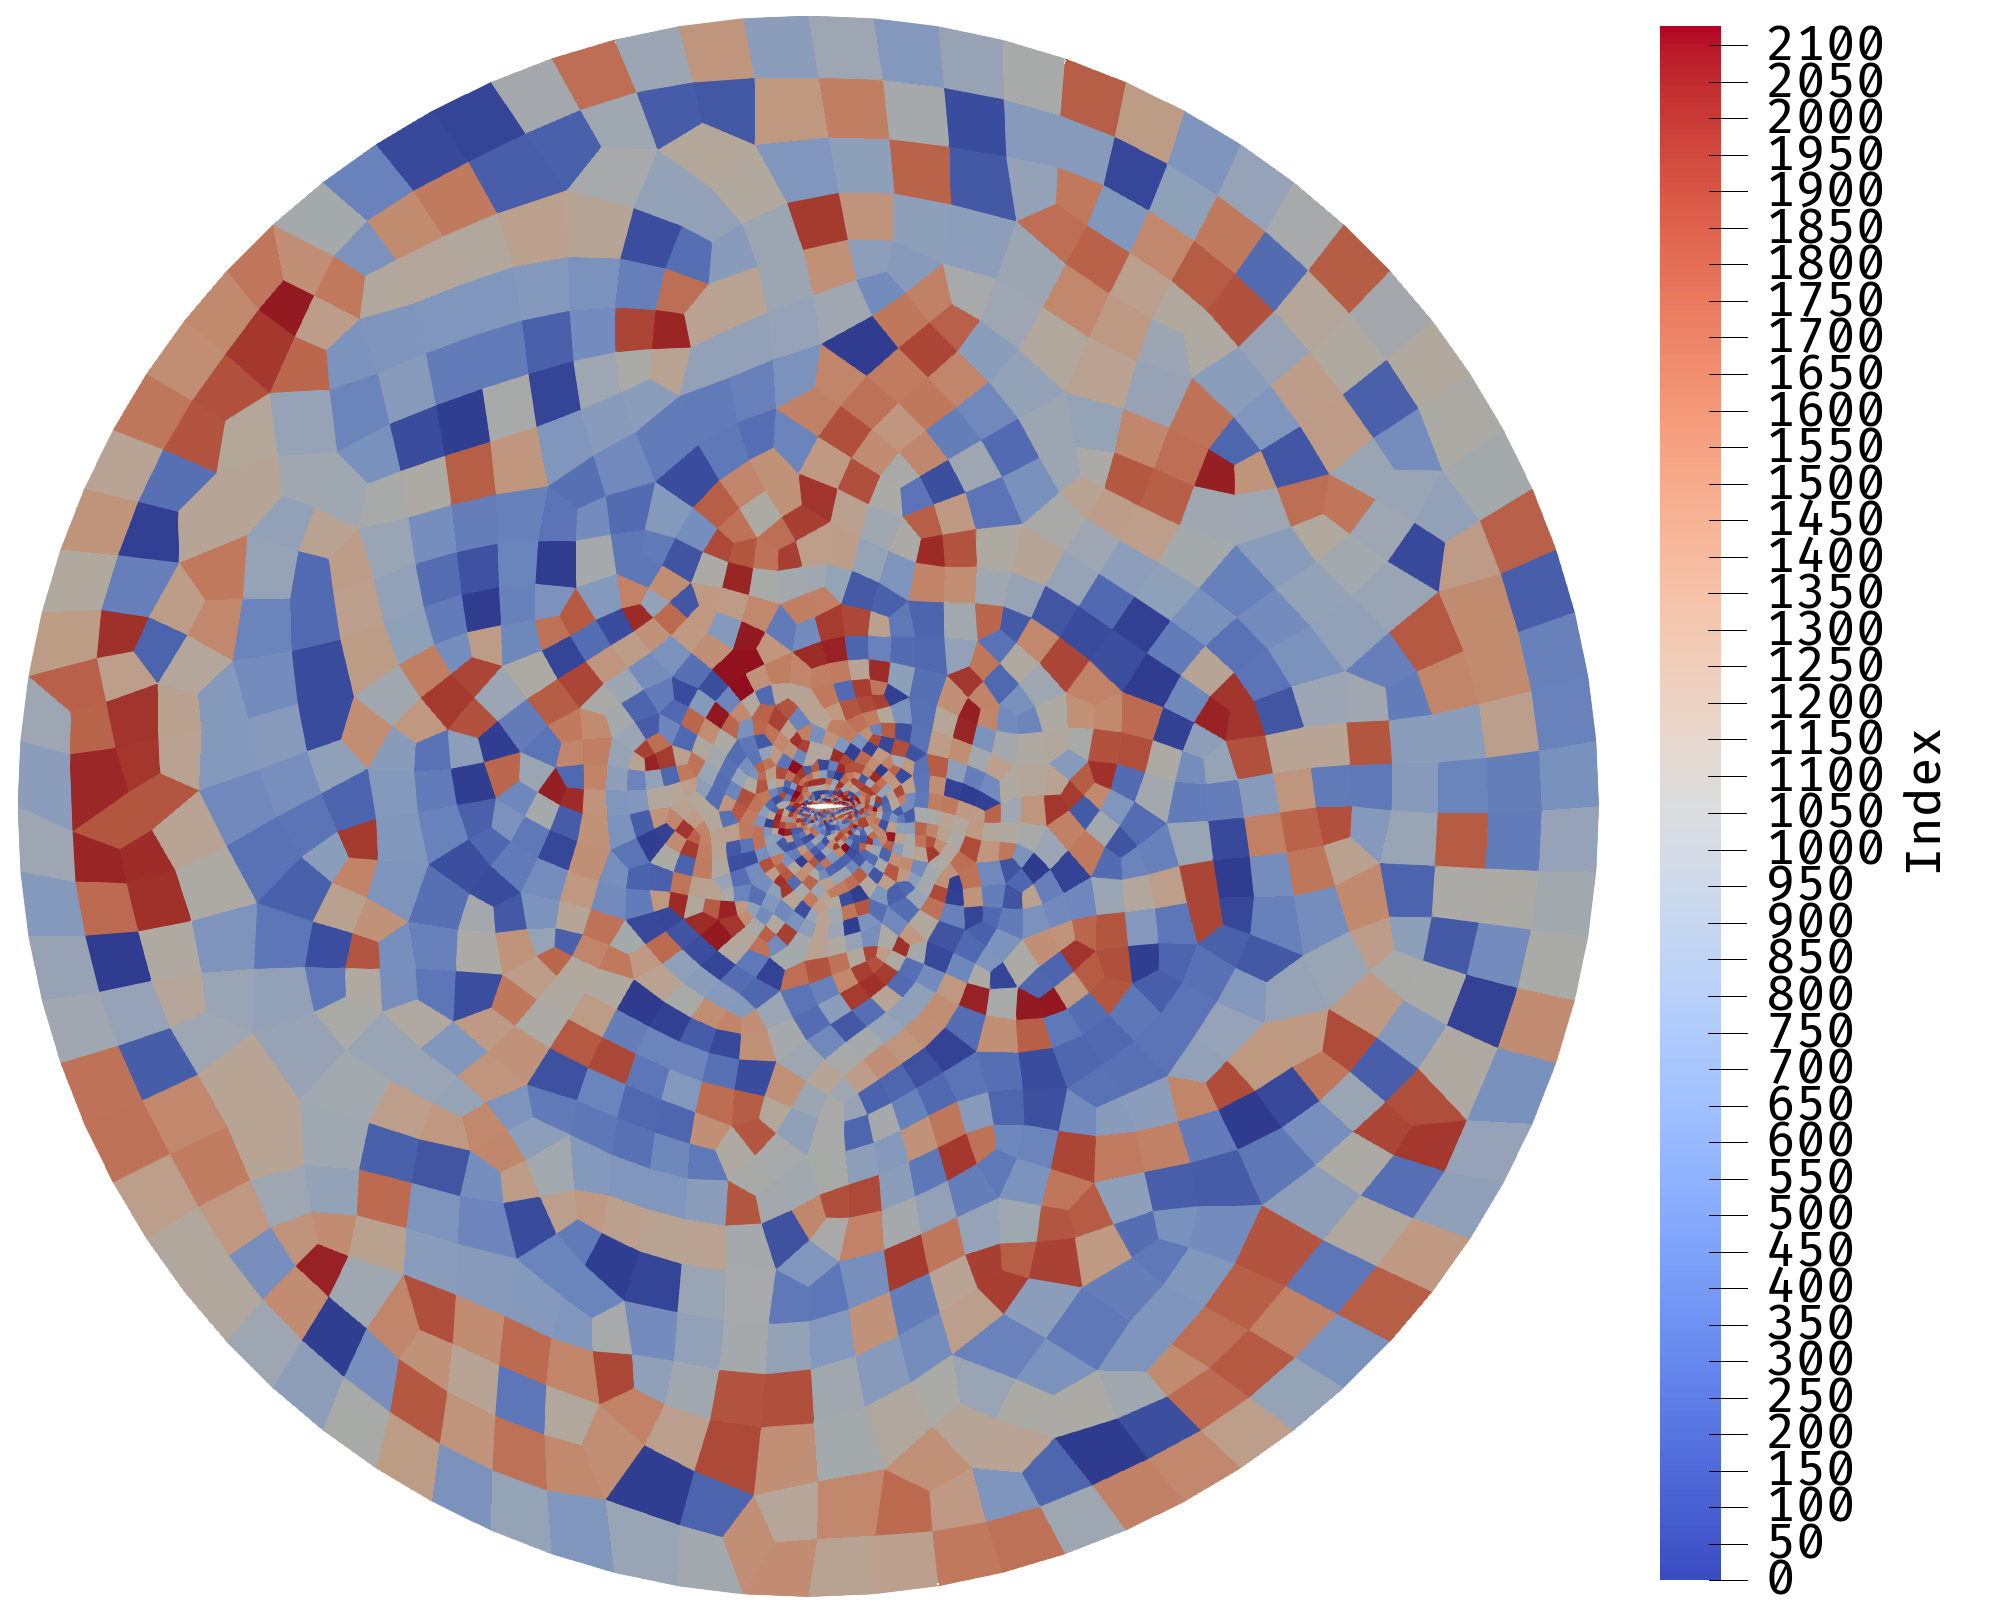
\includegraphics[width=0.45\textwidth]{Chapter_renumbering/media/ordering_unsorted}\label{fig:ordering_unsorted}}
	\subfloat[Rank]
	{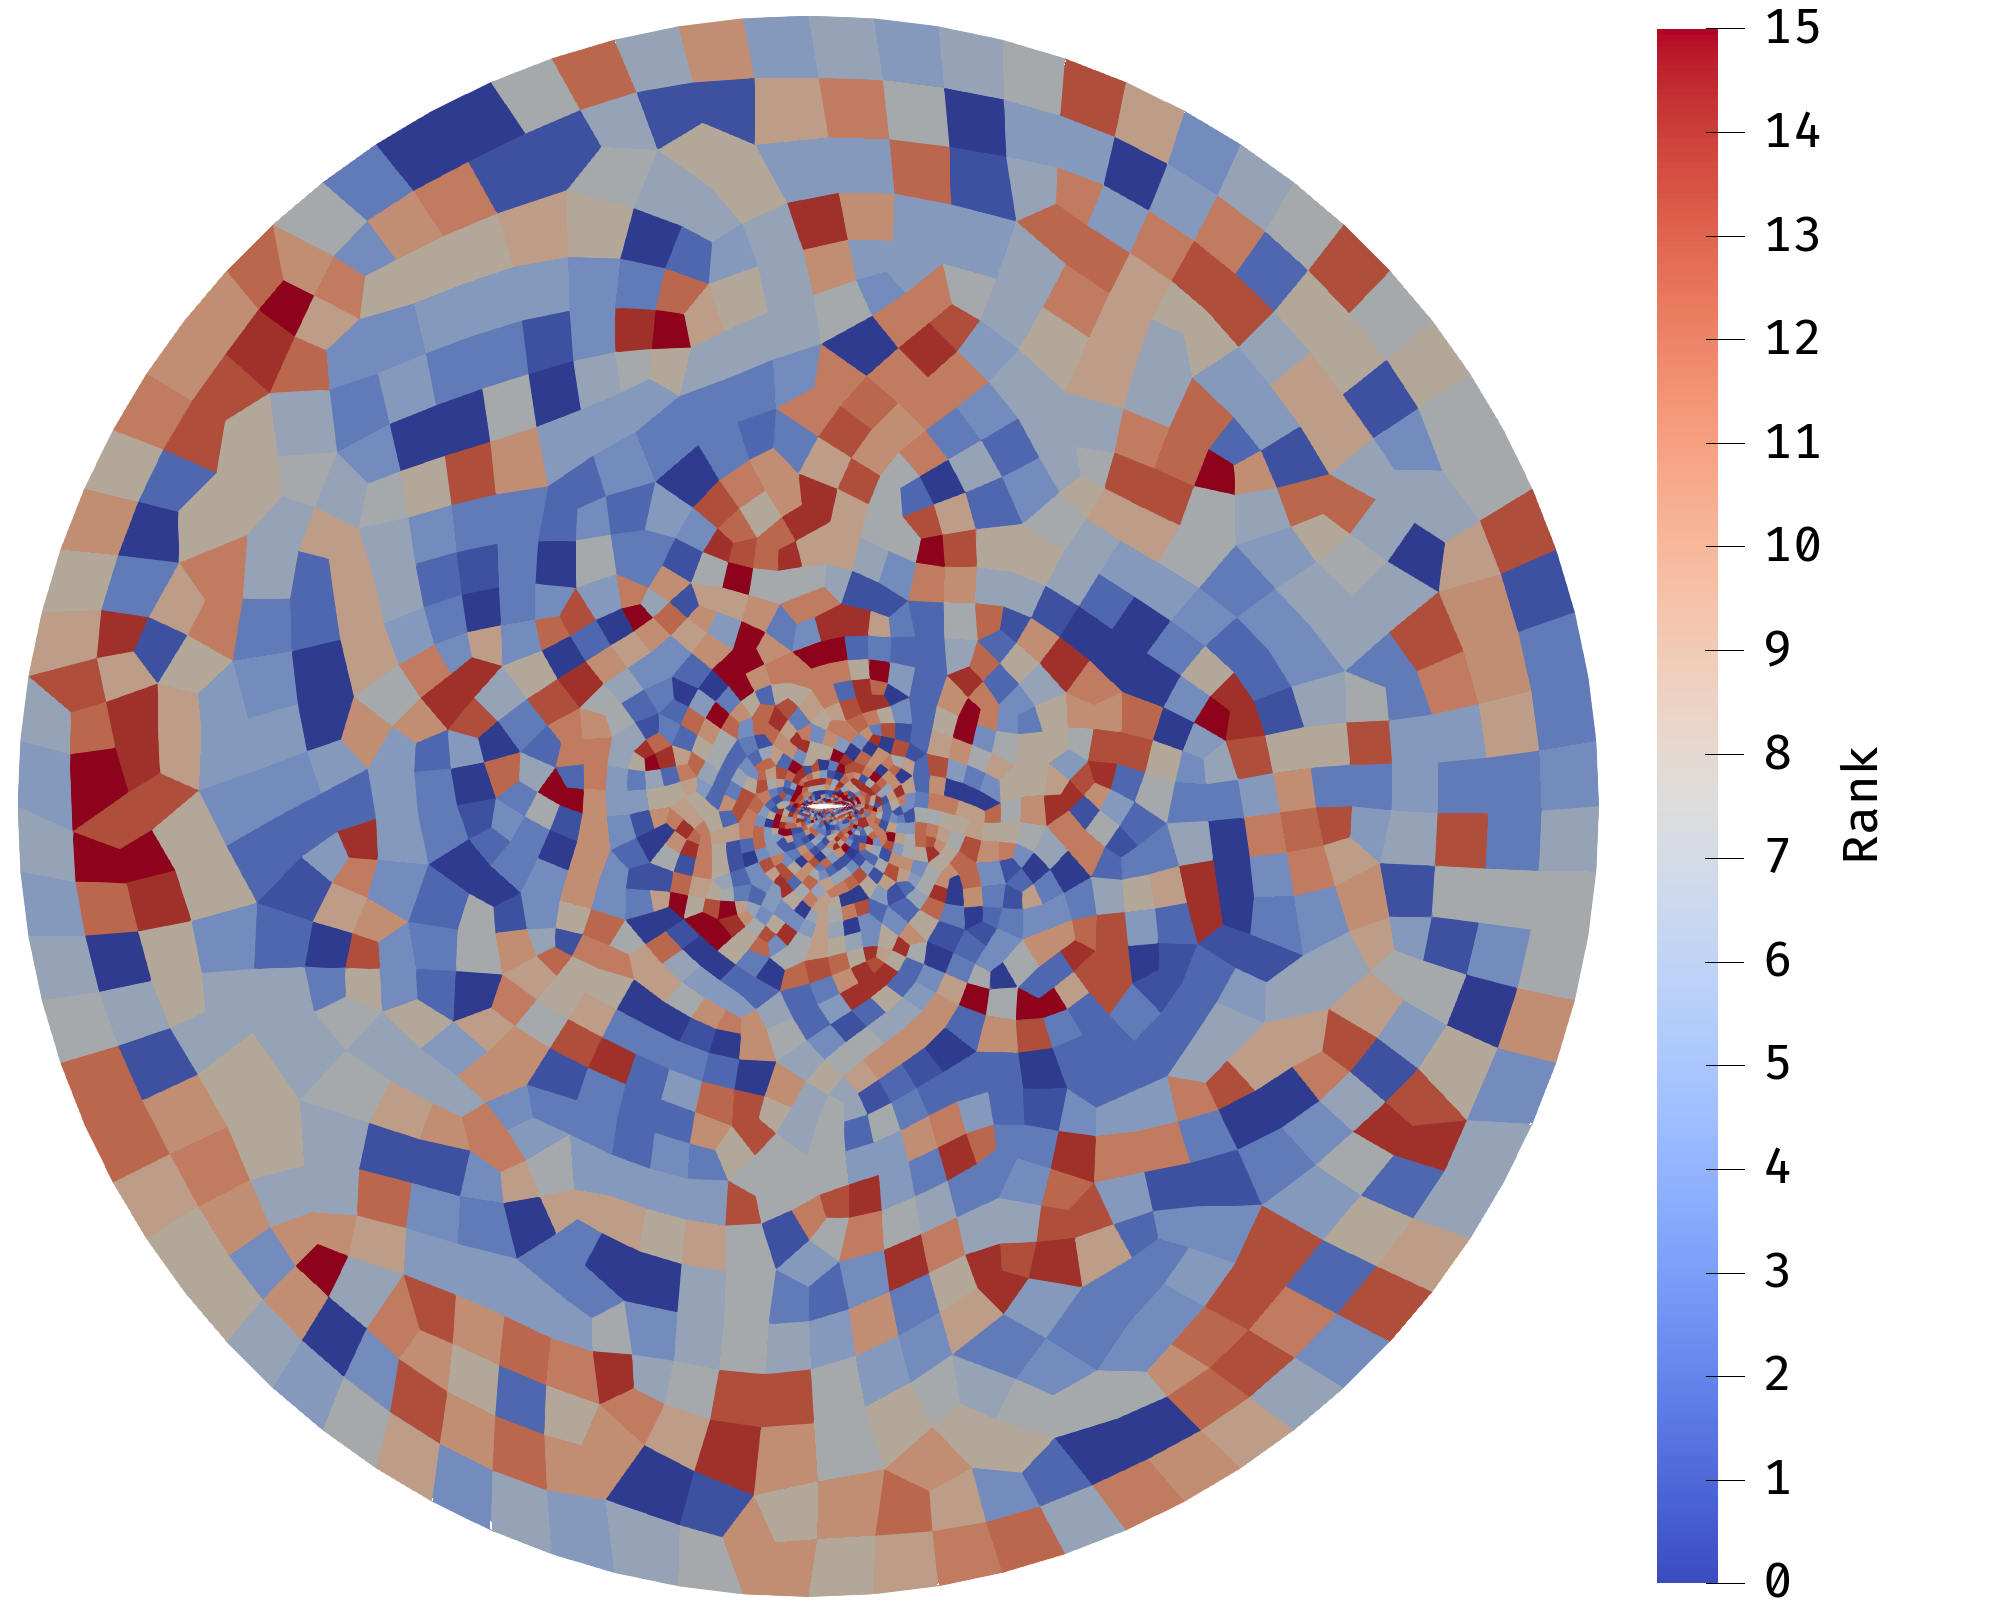
\includegraphics[width=0.45\textwidth]{Chapter_renumbering/media/rank_unsorted}\label{fig:rank_unsorted}}
	\caption{Unsorted mesh: The mesh is partitioned into \(16\) mesh blocks. (a) Ordering of the elements within the mesh (b) Mesh blocks once partitioned}\label{fig:mesh_unsorted}
\end{figure}

As we see, the resulting mesh blocks are scattered around the mesh, leading to unnecessarily large
boundaries between blocks. In order to get good performance, we will need to renumber the mesh. 

Since this mesh is circular, and the discontinuity representing the fuselage is in the middle, a
simple sorting algorithm could be to represent the elements in polar coordinates, and sort them
according to their angle around the center \(\theta \). Doing this, we get the ordering and
partitioning shown in Figure~\ref{fig:mesh_circular}.

\begin{figure}[H]
	\centering
	\subfloat[Ordering]
	{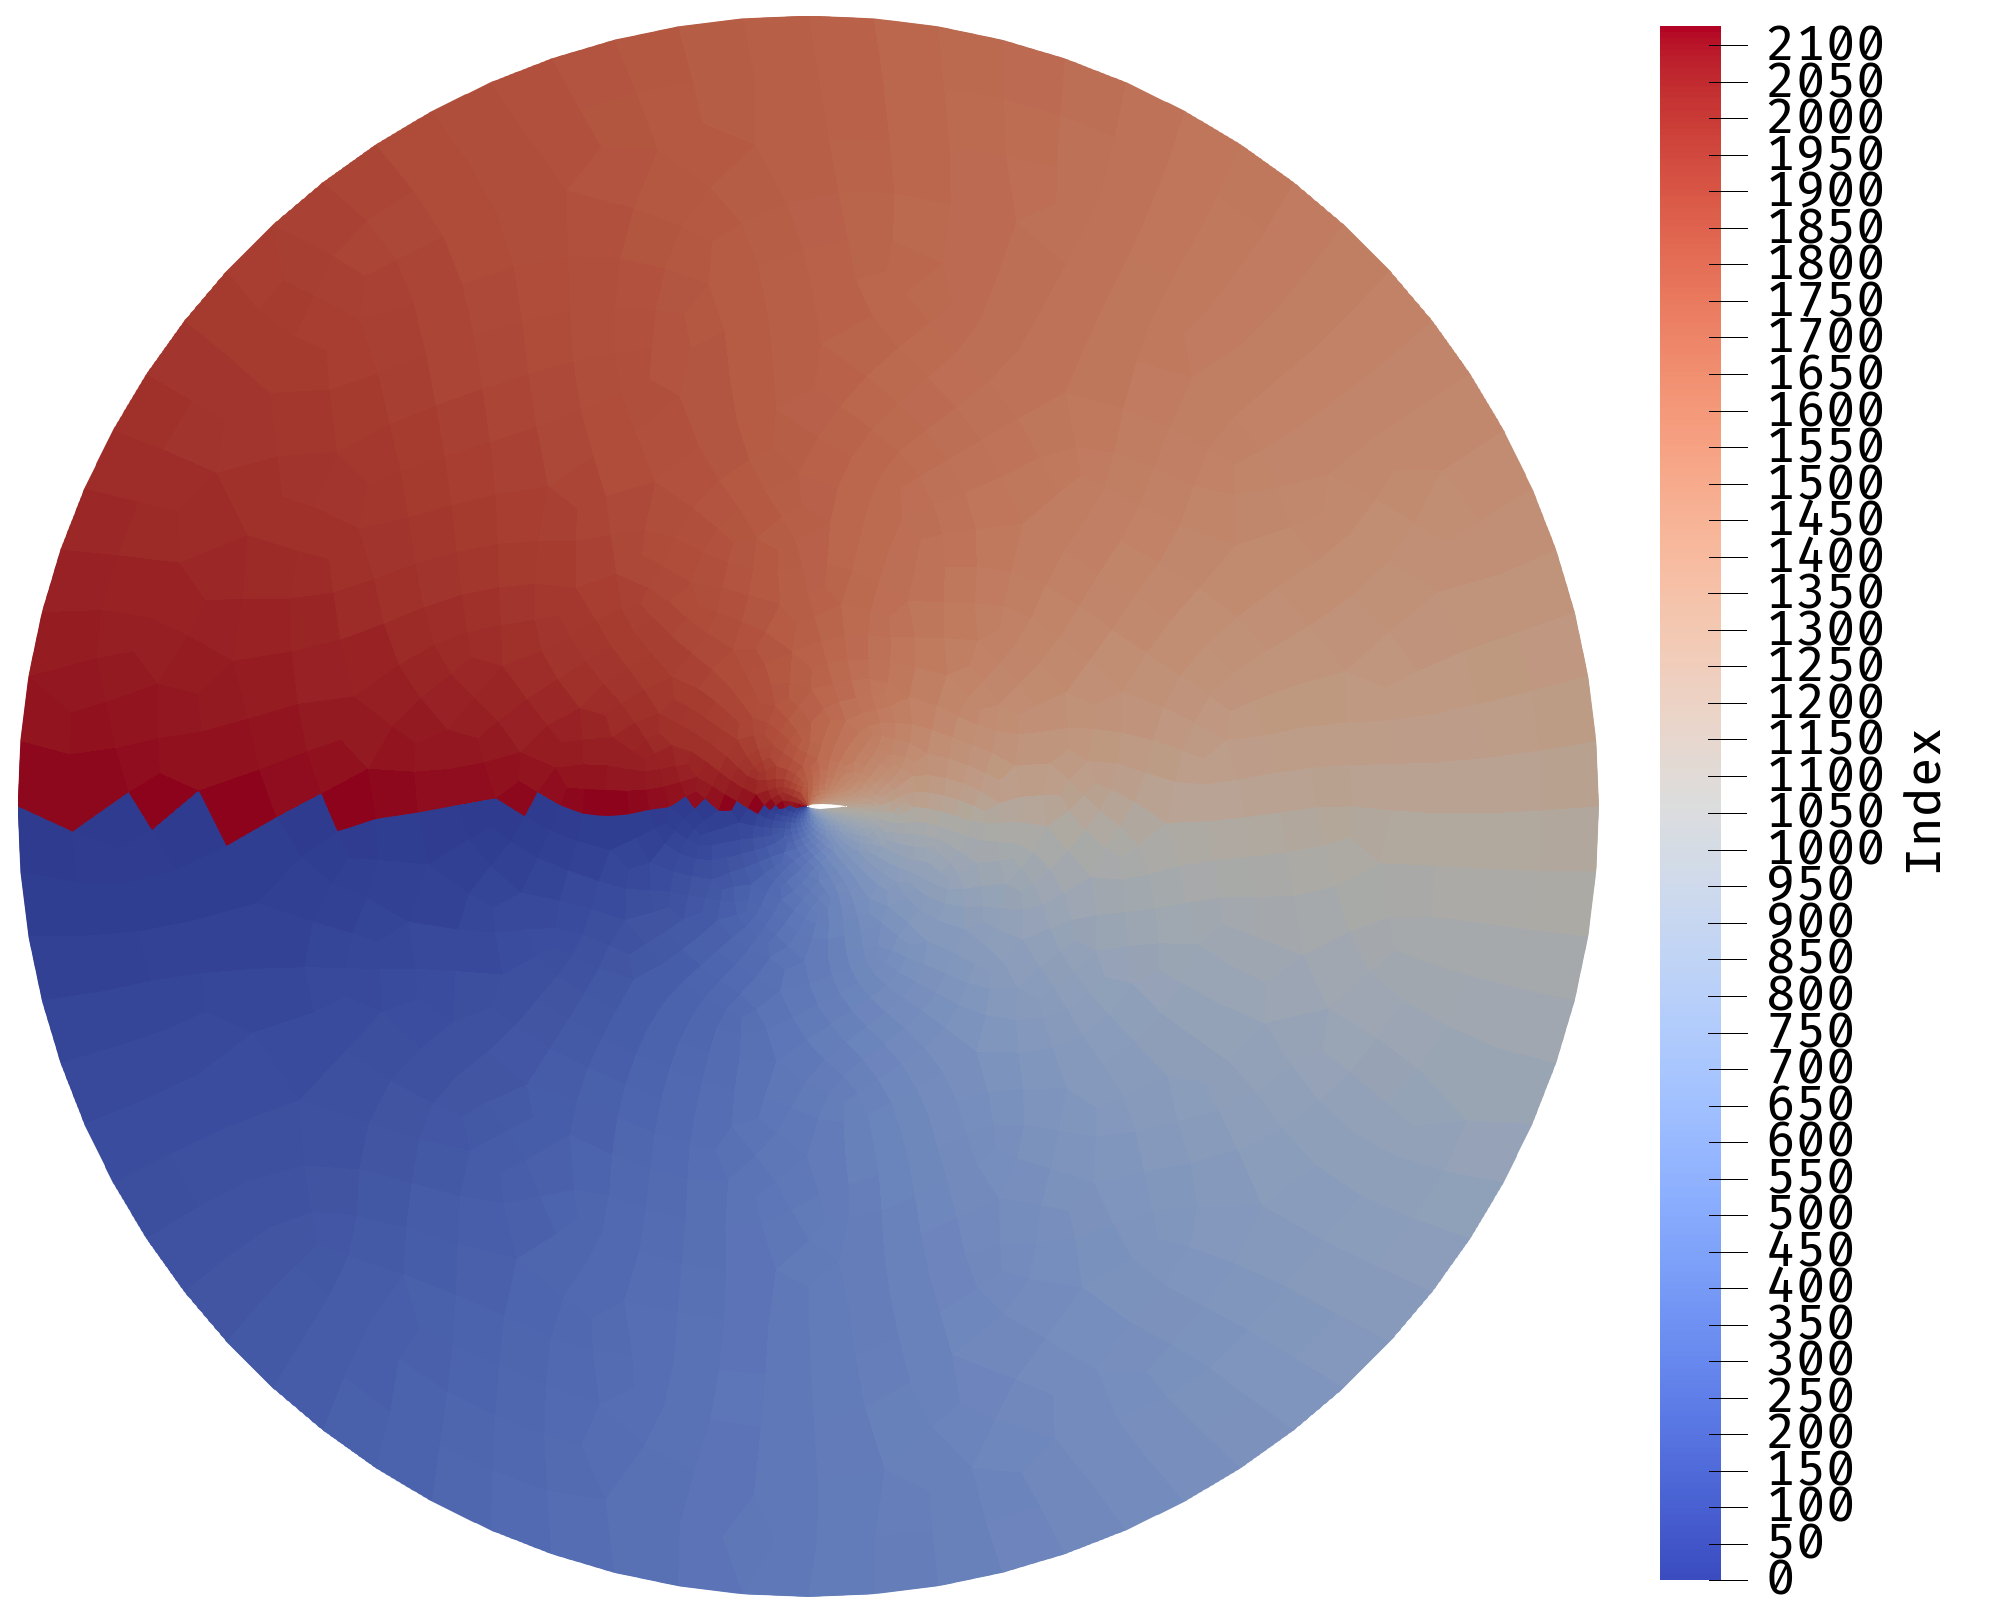
\includegraphics[width=0.45\textwidth]{Chapter_renumbering/media/ordering_circular}\label{fig:ordering_circular}}
	\subfloat[Rank]
	{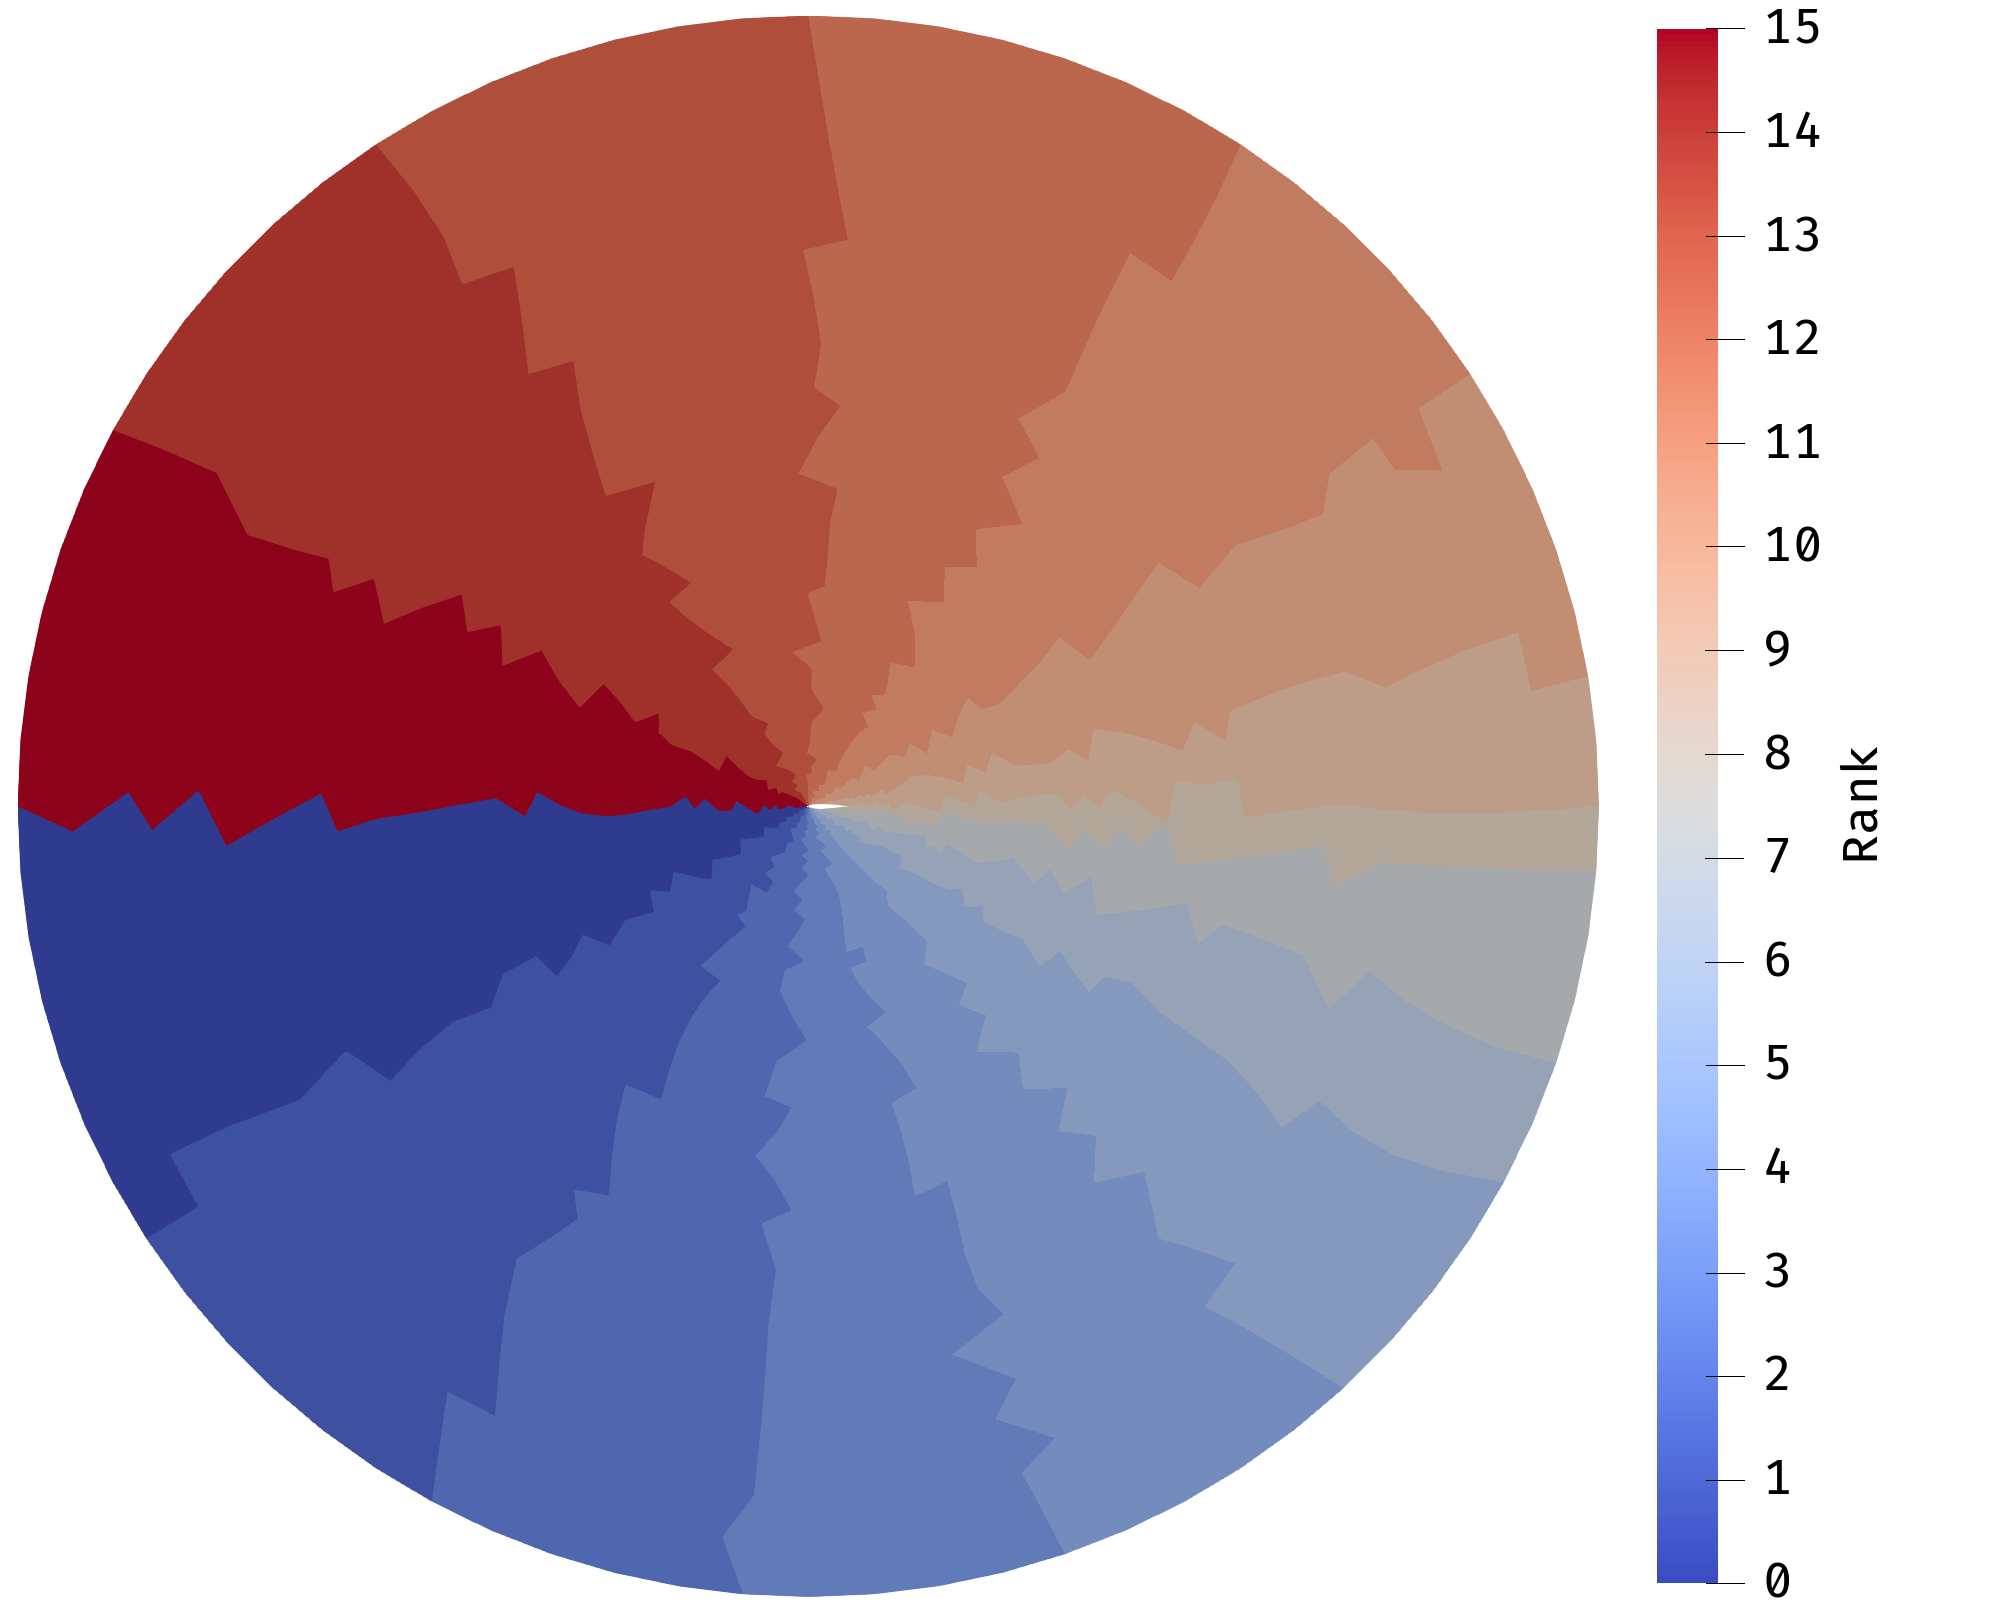
\includegraphics[width=0.45\textwidth]{Chapter_renumbering/media/rank_circular}\label{fig:rank_circular}}
	\caption{Circular sorted mesh: The elements are sorted according to their angle and the mesh is partitioned into \(16\) mesh blocks. (a) Ordering of the elements within the mesh (b) Mesh blocks once partitioned}\label{fig:mesh_circular}
\end{figure}

% doesn't work as well fof non-circles, good grouping but as there are more blocks they become thin
% slices with large boundaries. Then check next figure for how is locality, how elements are close
% their neighbours and numbered within blocks

\begin{figure}[H]
	\centering
	\includesvg[width=0.45\textwidth]{Chapter_renumbering/media/mesh_P0_before_adaptivity1_circular}
	\caption{Circular sorted mesh element ordering: The elements are very far from their neighbours.}\label{fig:mesh_circular_ordering}
\end{figure}

% is no good

% Figure about how we do it, that the curve is not defined but we map too square, make hilbert curve
% and sort elements according to into which index they fall. If multiple are in the same they keep
% their relative order. This is why we make very fine Hilbert curve

% figure about how we do it

% This is the ordering and blocks it gives

\begin{figure}[H]
	\centering
	\subfloat[Ordering]
	{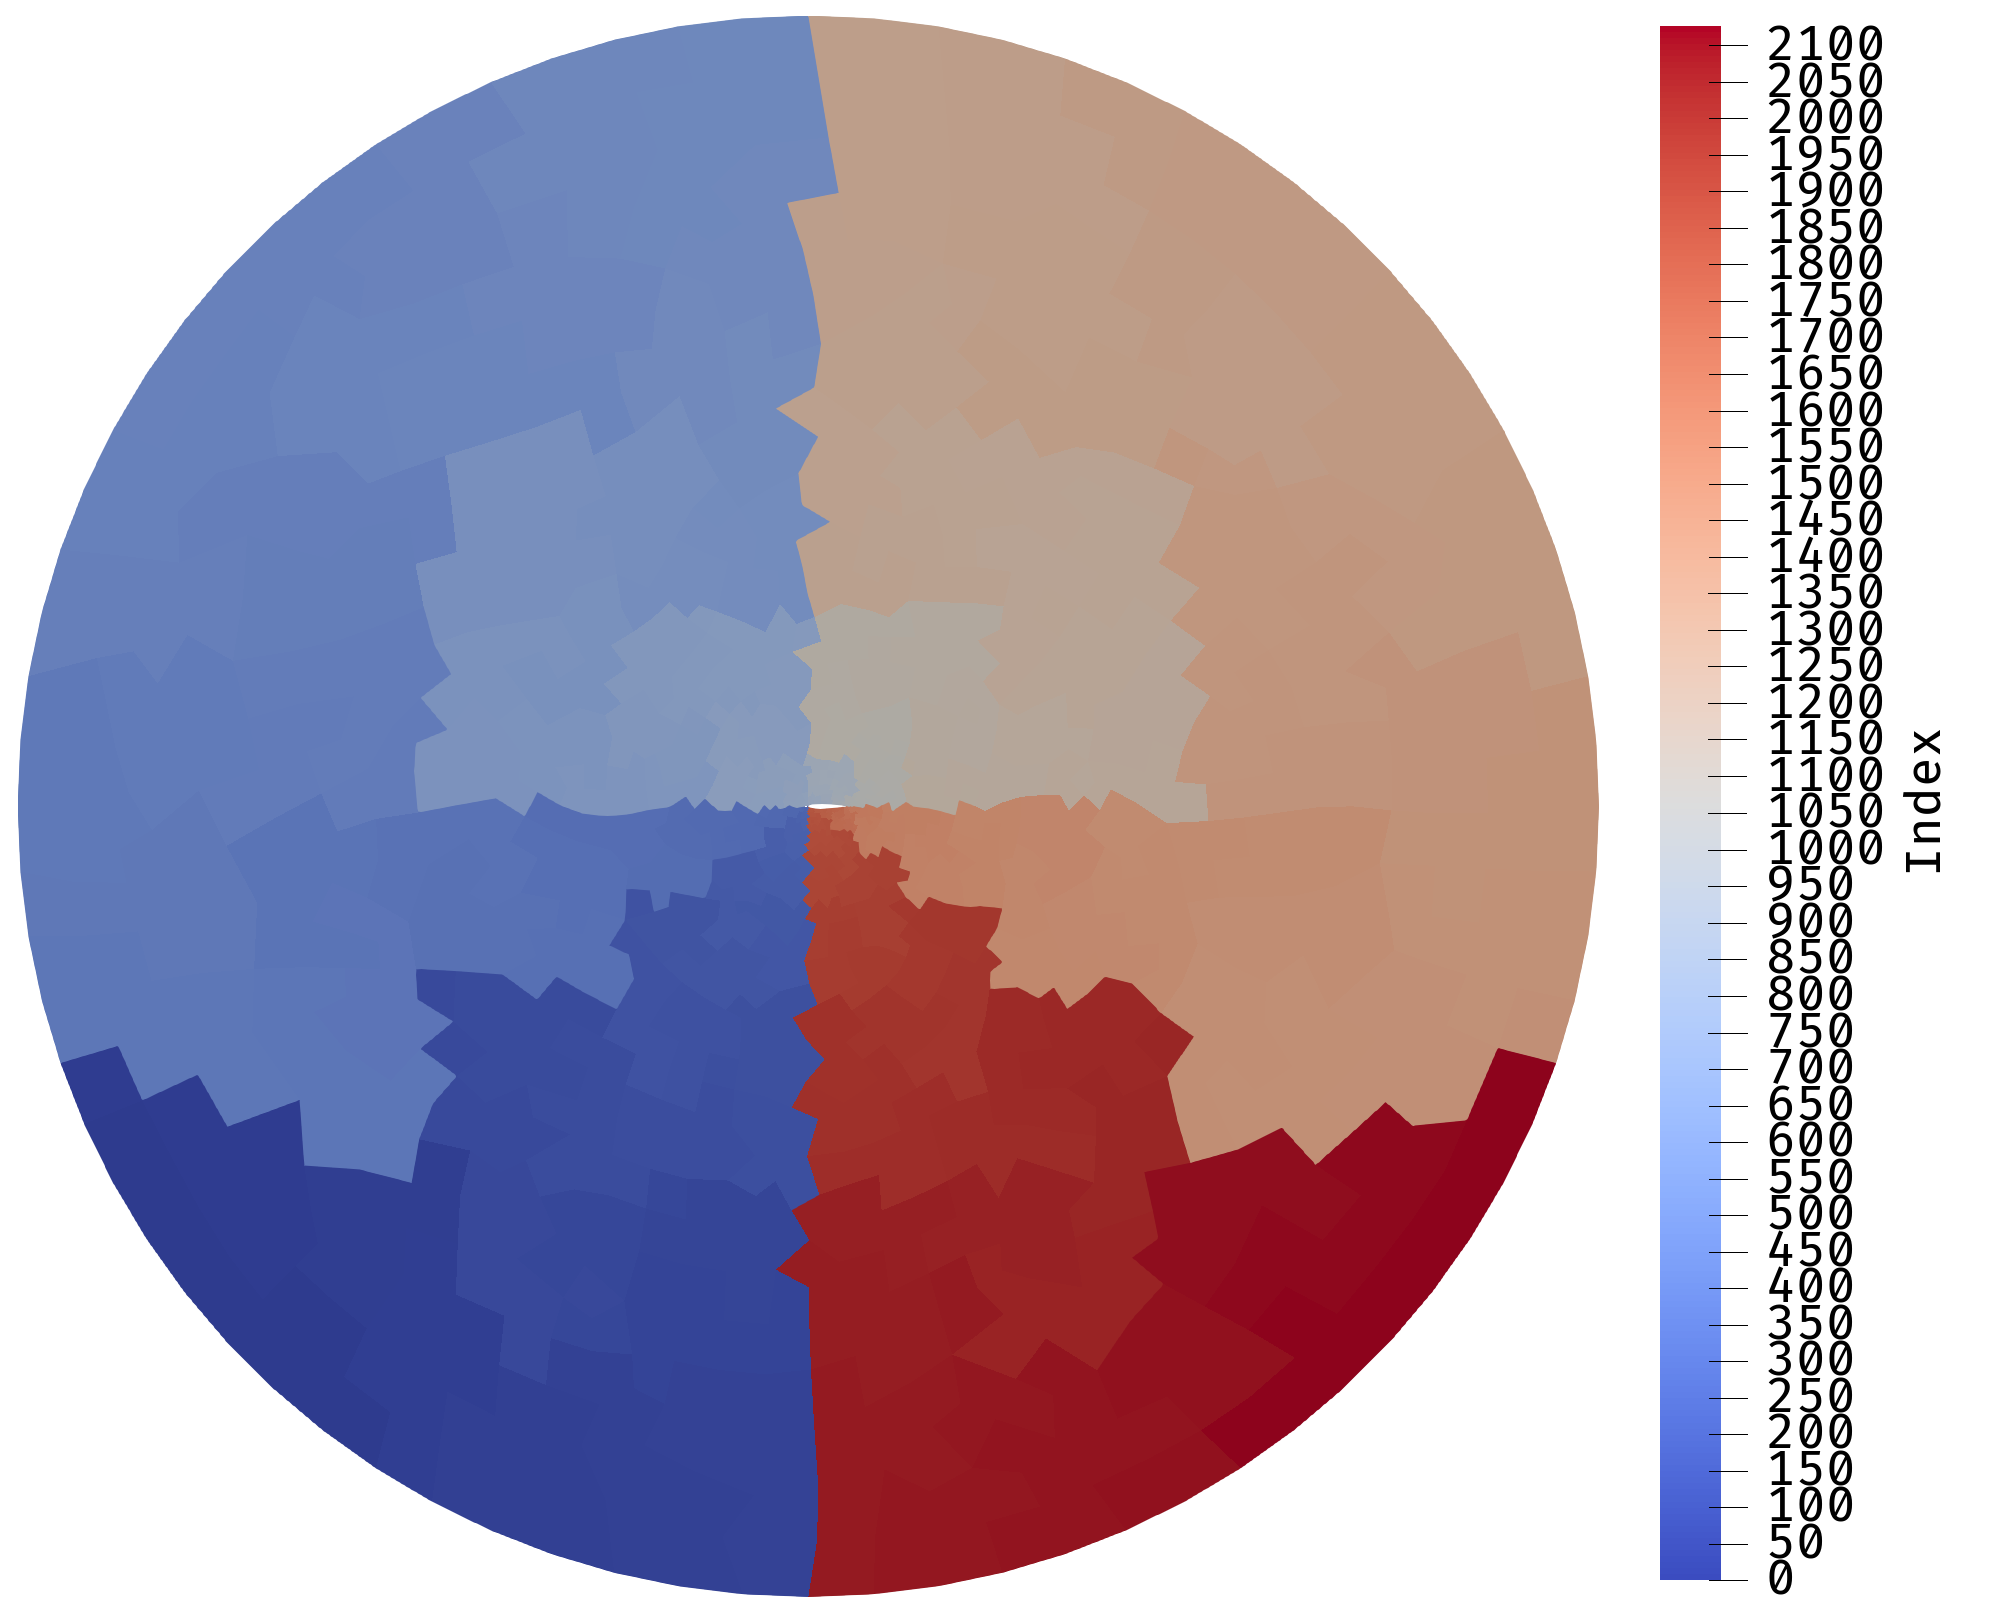
\includegraphics[width=0.45\textwidth]{Chapter_renumbering/media/ordering_hilbert}\label{fig:ordering_hilbert}}
	\subfloat[Rank]
	{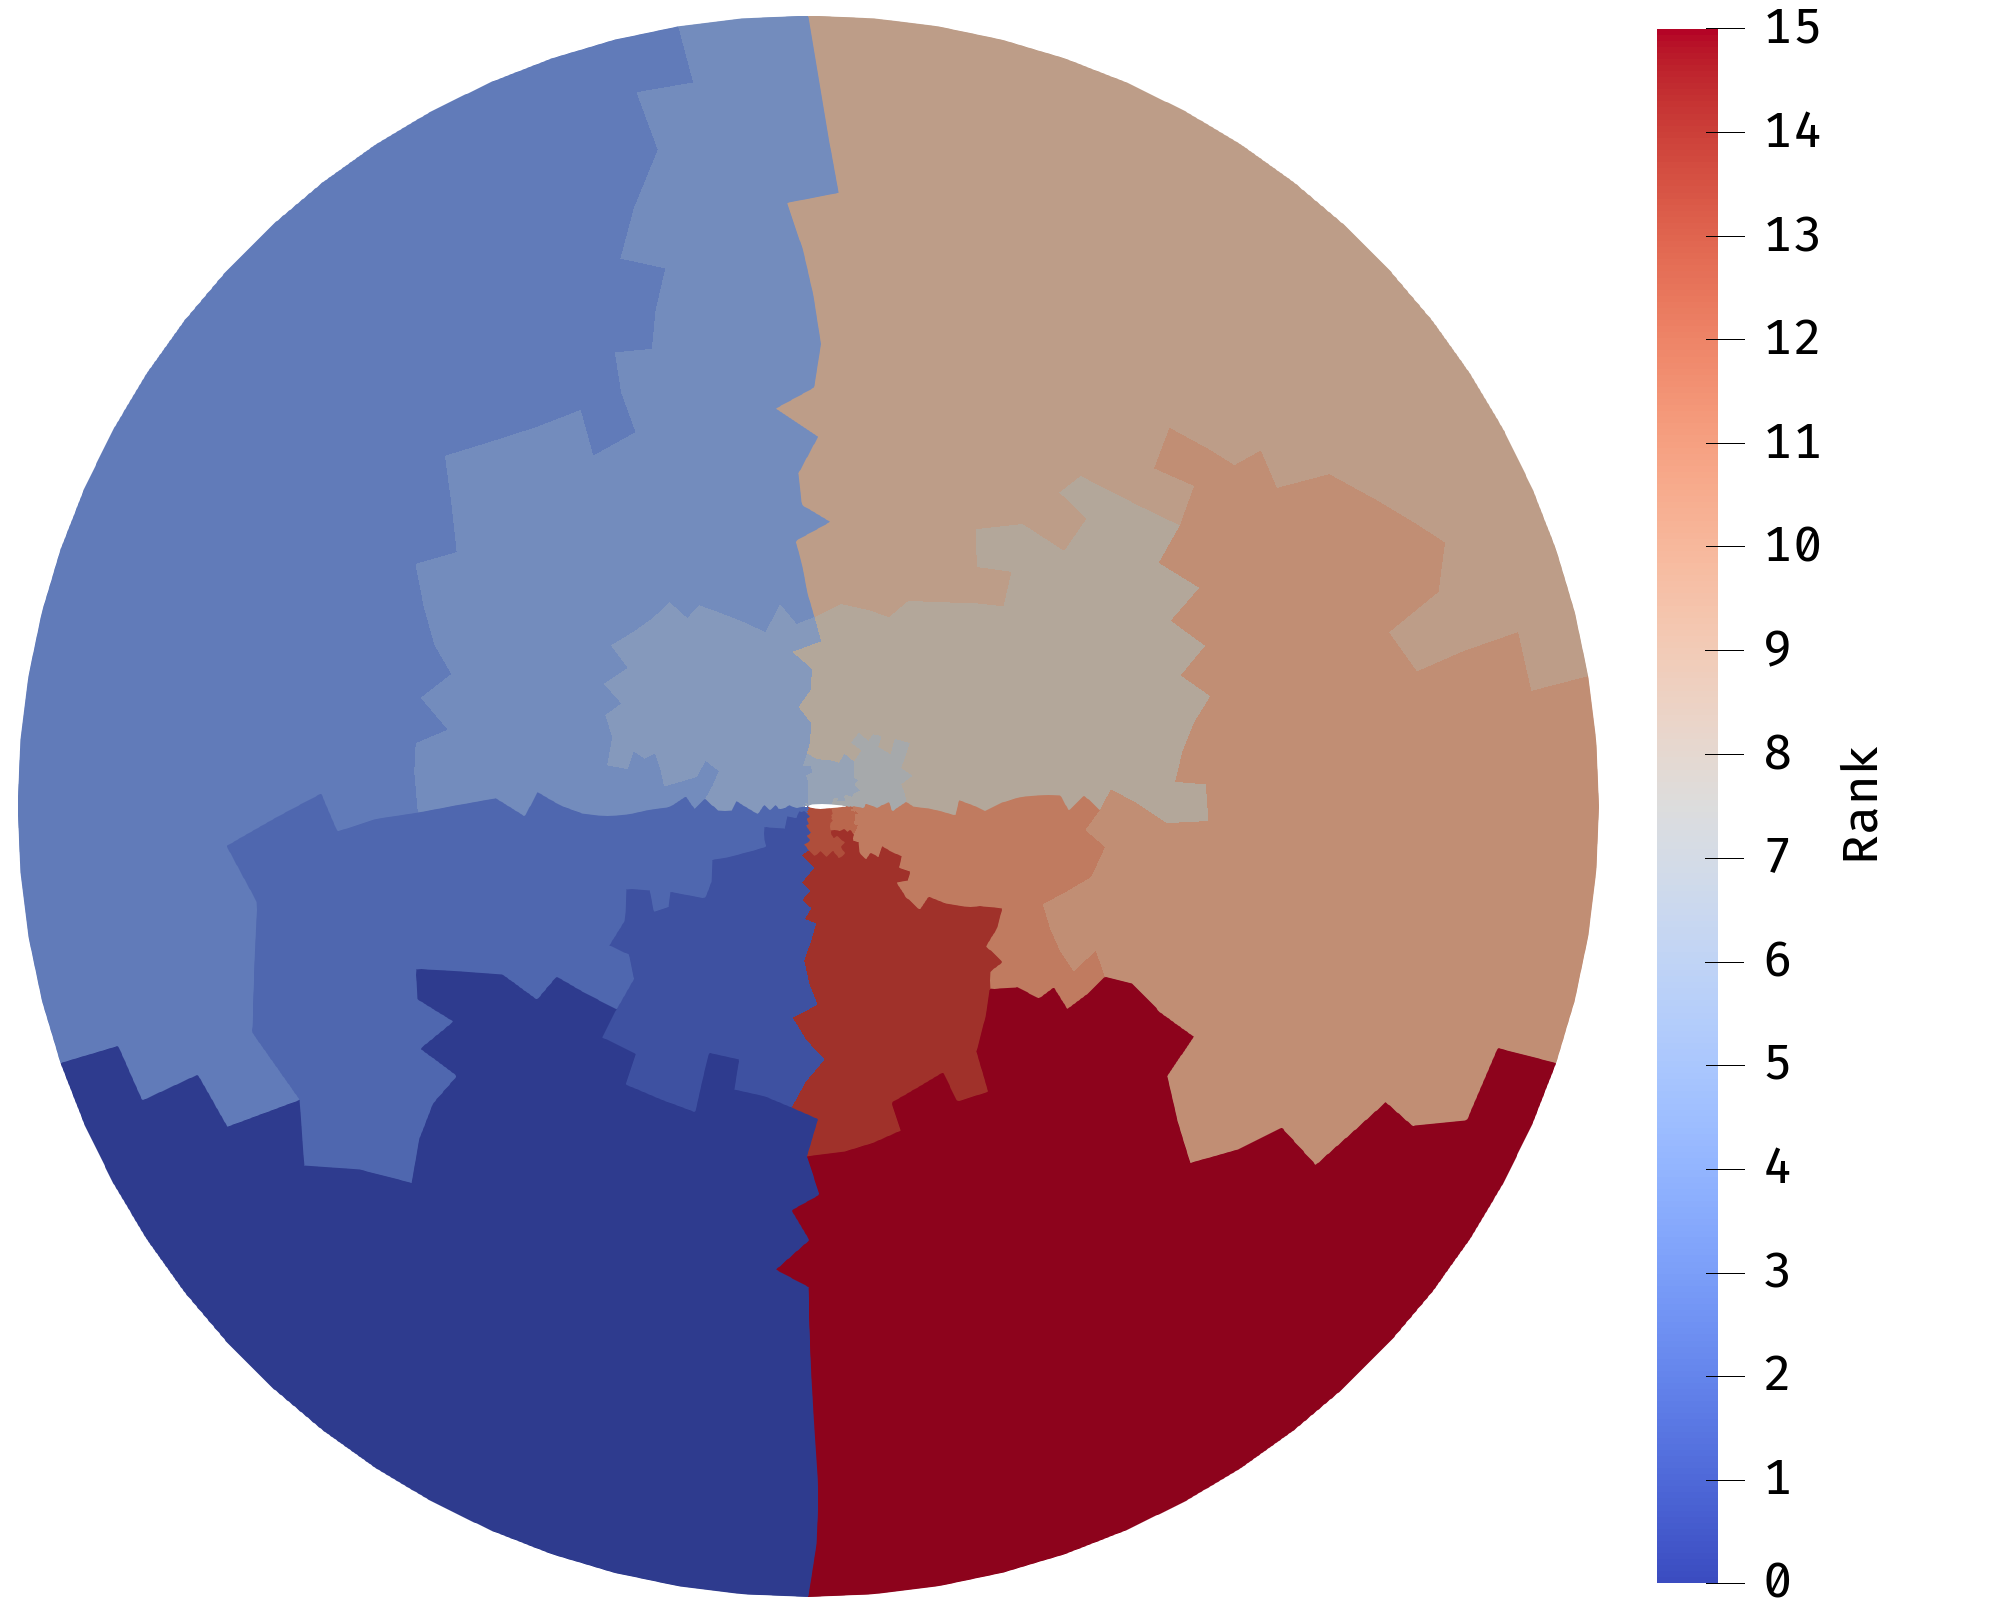
\includegraphics[width=0.45\textwidth]{Chapter_renumbering/media/rank_hilbert}\label{fig:rank_hilbert}}
	\caption{Pseudo-Hilbert sorted mesh:The elements are sorted according to their index along a Hilbert curve, and the mesh is partitioned into \(16\) mesh blocks. (a) Ordering of the elements within the mesh (b) Mesh blocks once partitioned}\label{fig:mesh_hilbert}
\end{figure}

% Good, good grouping elements and looks a bit like the real curve from ref{}
% Then we show the next figures, how is the ordering and how it works for refinement

\begin{figure}[H]
	\centering
	\subfloat[Before refinement]
	{\includesvg[width=0.45\textwidth]{Chapter_renumbering/media/mesh_P0_before_adaptivity1}\label{fig:mesh_P0_before_adaptivity1_far}}
	\subfloat[After refinement]
	{\includesvg[width=0.45\textwidth]{Chapter_renumbering/media/mesh_P0_after_adaptivity1}\label{fig:mesh_P0_after_adaptivity1_far}}
	\caption{\Acrlong{acr:AMR} with an unstructured mesh: The mesh is refined, created elements follow the initial pseudo-Hilbert curve. (a) Initial mesh (b) Mesh after a single refinement step}\label{fig:mesh_P0_adaptivity_far}
\end{figure}

\begin{figure}[H]
	\centering
	\subfloat[Solution time]
	{\includesvg[width=0.45\textwidth]{Chapter_renumbering/media/mesh_P0_before_adaptivity1_near}\label{fig:mesh_P0_before_adaptivity1_near}}
	\subfloat[Maximum error]
	{\includesvg[width=0.45\textwidth]{Chapter_renumbering/media/mesh_P0_after_adaptivity1_near}\label{fig:mesh_P0_after_adaptivity1_near}}
	\caption{\Acrlong{acr:AMR} with an unstructured mesh (detail): The mesh is refined, created elements follow the initial pseudo-Hilbert curve. There are jumps along the curve around the fuselage. (a) Initial mesh (b) Mesh after a single refinement step}\label{fig:mesh_P0_adaptivity_near}
\end{figure}

% Very good, refinement keeps the order of the curve well
% The order of the curve is good, but there are discontinuities near airfoil and weird jumps.
% Discontinuities: curve is not defined to have holes. Not too bad in this case since hole in middle
% Weird jumps:
% When too fine, the curve will "miss" elements by a little, giving surprising results. Future work:
% do with coarse grid, and refine for elements that fall in the same index only until they do not.

    \chapter{Hybrid Solver}\label{chapter:hybrid_solver}

In this work, we use \acrshortpl{acr:GPU} to accelerate spectral methods. We use
\acrshortpl{acr:GPU} because they have a higher parallel throughput that traditional
\acrshortpl{acr:CPU}. We have shown that we can gain up to around three times the performance of
\acrshortpl{acr:CPU} on \acrshort{acr:HPC} systems in Section~\ref{section:results:scaling_tests}.

By that metric, by using only \acrshortpl{acr:GPU} we leave \(25 \% \) of the performance of those
systems on the table. While we perform computations on \acrshortpl{acr:GPU}, each \acrshort{acr:GPU}
is paired with a \acrshort{acr:CPU} core to feed it data and instructions, while the other
\acrshort{acr:CPU} cores are left idle. If we could design a program that uses both
\acrshortpl{acr:GPU} and \acrshortpl{acr:CPU} for computations, we could unlock the full processing
power of those \acrshort{acr:HPC} systems. This appendix describes a heterogeneous \textit{hybrid
solver} that uses both \acrshortpl{acr:CPU} and \acrshortpl{acr:GPU} to compute the solution.

In this work, we implemented a \acrshort{acr:CPU} version of the program to perform the
\acrshort{acr:CPU}-\acrshort{acr:GPU} comparison for Section~\ref{section:results:scaling_tests}.
Both versions use the same interface to communicate between processes via \acrshort{acr:MPI}, which
means it was simple to make them work together heterogeneously. To pick the kind of worker a process
is, we launch multiple processes via \acrshort{acr:MPI}. The first processes pick \acrshort{acr:GPU}
devices until there are none remaining in the system and execute the \acrshort{acr:GPU} version of
the code, and the remaining processes execute the \acrshort{acr:CPU} version of the code.

The work now needs to be partitioned between \acrshortpl{acr:CPU} and \acrshortpl{acr:GPU}. Since
those two types of processors have vastly different capabilities, the partition must be uneven in
order to obtain the best performance. Section~\ref{section:load_balancing:workload_leveling}
describes the algorithm to repartition a 1D workload. At the end of the section, we make the
assumption that all workers have the same capacity to simplify the equation. This is no longer the
case if we can have both \acrshort{acr:CPU} and \acrshort{acr:GPU} workers. We will use
Equation~\ref{equ:ideal_workload} to separate the work between workers. It states:

\begin{equation}
	w_{ideal,p} = W \frac{c_p}{C},
\end{equation}

\noindent
where \(W\) is the total workload, \(C\) is the total capacity, \(p\) is a worker index, \(c_p\) is
the capacity of worker \(p\), and \(w_{ideal,p}\) is the ideal workload for worker \(p\). We can
easily find \(W\) by summing the number of elements in the problem, and \(C\) by summing the
capacity of each worker. The capacity of each worker, representing the relative speed at which it
solves problems or the number of elements it can compute in the same time as others, is the only
unknown. This is the quantity that must be different for \acrshortpl{acr:CPU} and
\acrshortpl{acr:GPU}.

For the purpose of this quick exploration of hybrid solvers, we will use a simple heuristic to
determine the relative capacity of \acrshortpl{acr:CPU} and \acrshortpl{acr:GPU}. We run a simple
case with one \acrshort{acr:GPU} and time its execution, then do the same with a single
\acrshort{acr:CPU}. This gives us the performance ratio between the two types of workers. On the
consumer platform described in Subsection~\ref{subsection:results:platforms:consumer}, the ratio
amounts to about \(16\). This means that a \acrshort{acr:GPU} solves the problem \(16 \times \)
faster that a single \acrshort{acr:CPU} core, and should solve it in the same time as \(16\)
\acrshort{acr:CPU} cores. We give a capacity of \(16\) to \acrshort{acr:GPU} workers, and of one to
\acrshort{acr:CPU} workers.

We use the same test case from Section~\ref{section:results:test_case} to examine the hybrid version
of the program. We use the platform described in
Subsection~\ref{subsection:results:platforms:consumer}, with \(32\) \acrshort{acr:CPU} cores and one
\acrshort{acr:GPU}. We use a mesh with \(64\) elements in the \(x\) and \(y\) direction, and a
polynomial order \(N\) of four. Figure~\ref{fig:hybrid_load_balancing} shows the mesh partitioning
after load balancing.

\begin{figure}[H]
	\centering
	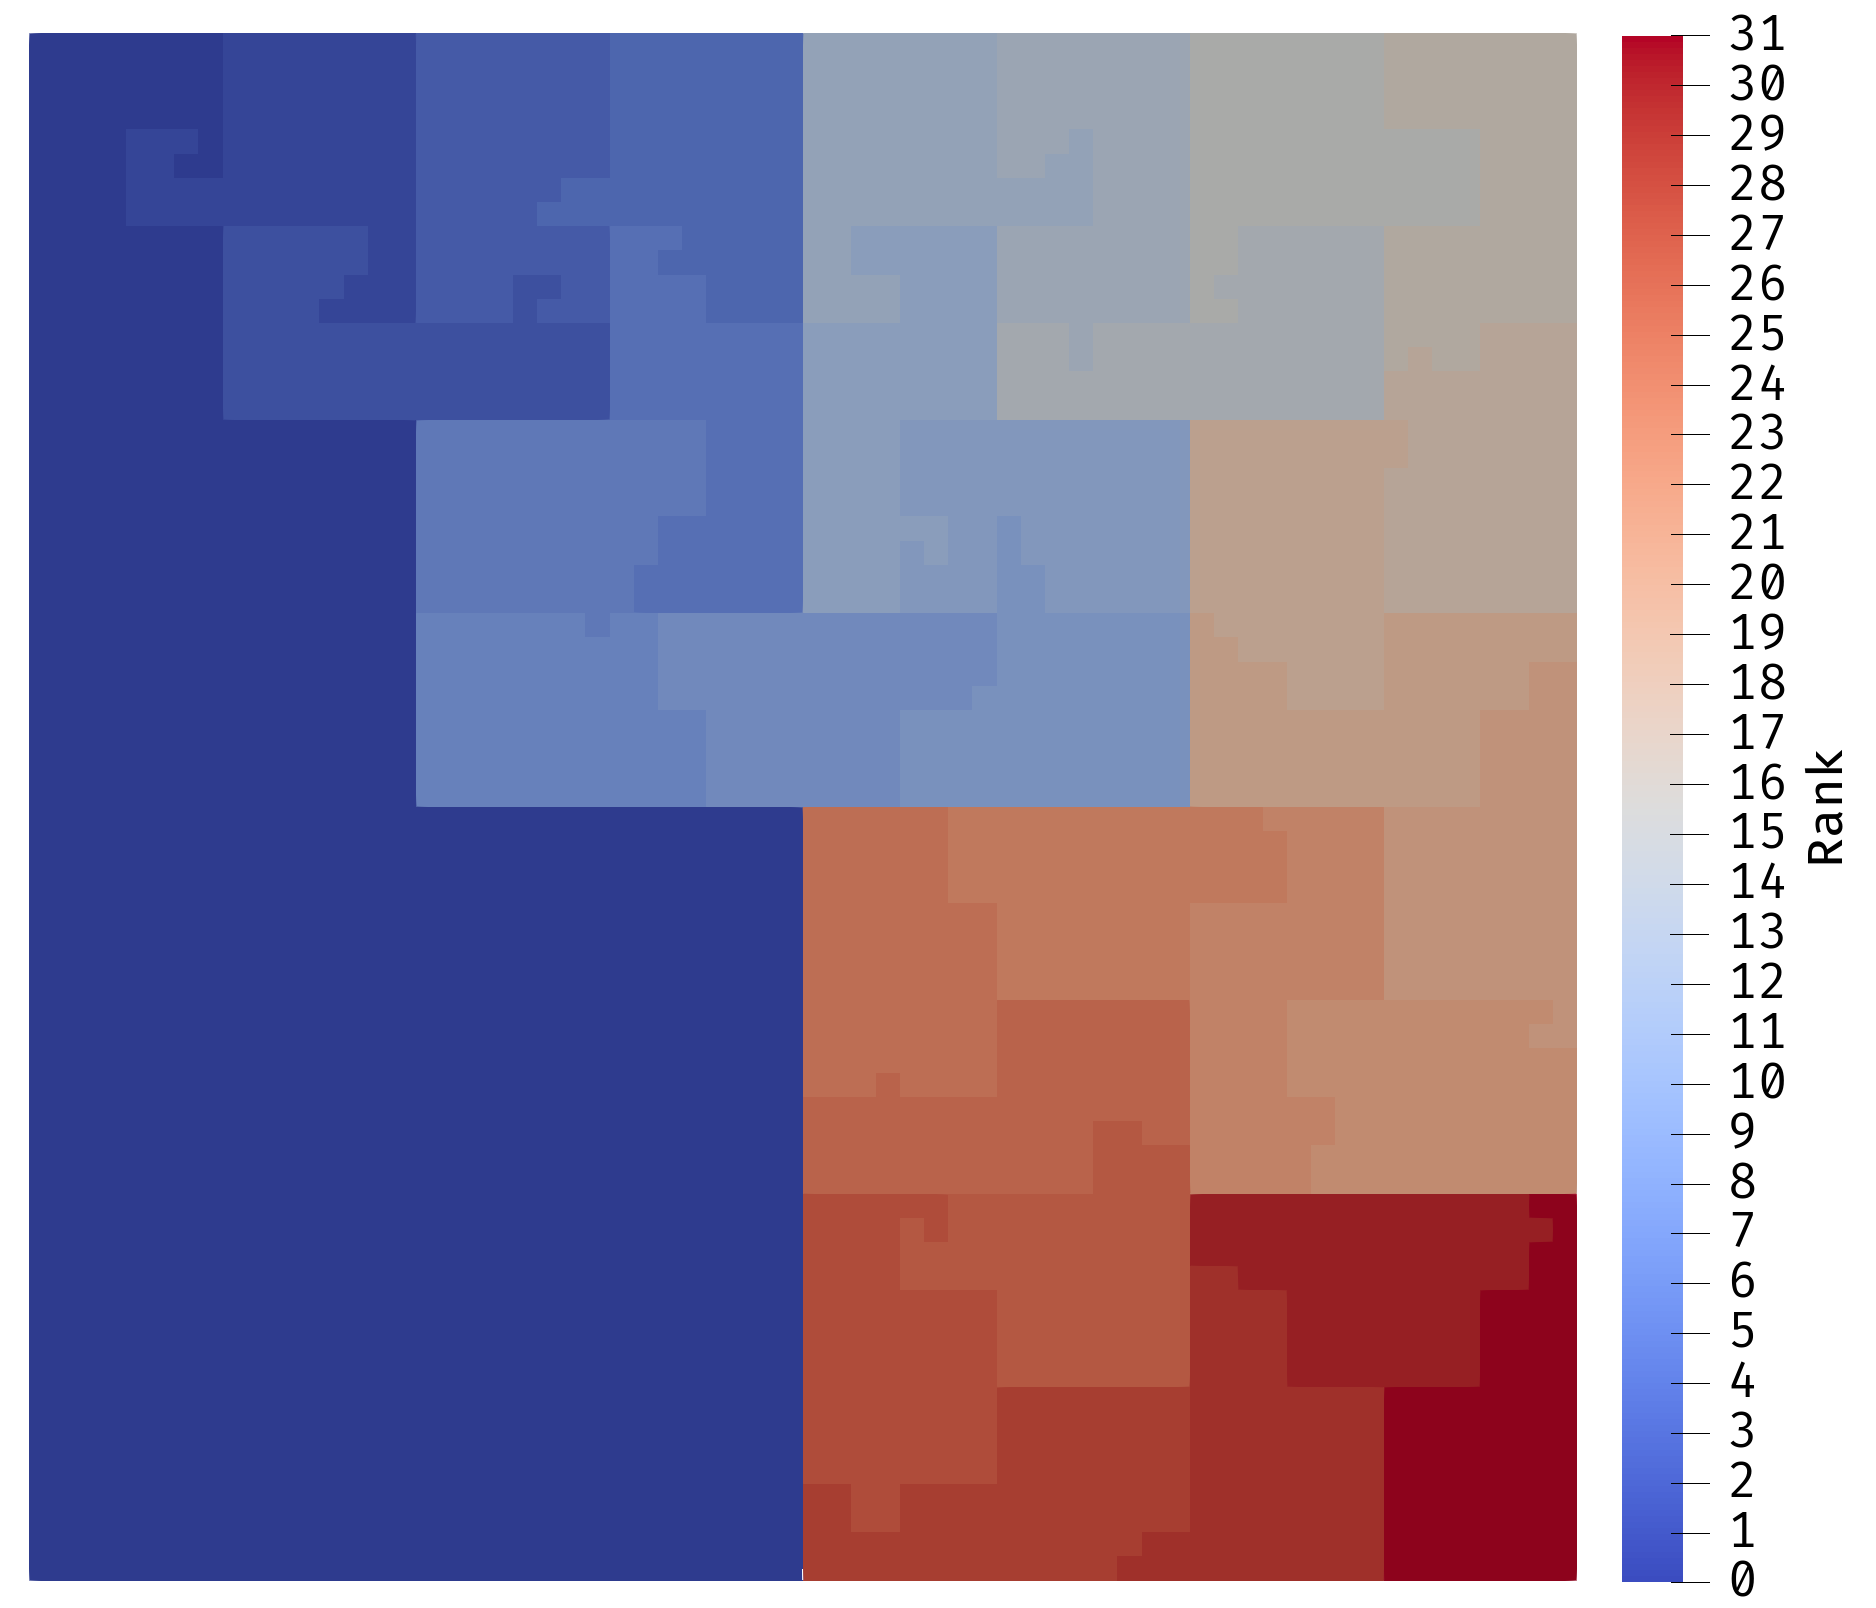
\includegraphics[width=0.65\textwidth]{Chapter_hybrid_solver/media/cpu_gpu}
	\caption{Load balancing with heterogenous workers: The first worker is a \acrshort{acr:GPU} and has more elements in its mesh block.}\label{fig:hybrid_load_balancing}
\end{figure}

Figure~\ref{fig:hybrid_load_balancing} shows that the first worker, with a rank of zero, has much
more elements in its mesh block than the other workers. The first worker is a \acrshort{acr:GPU},
and as such should have \(16\) times as many elements as the other workers. Along with \(31\)
\acrshort{acr:CPU} workers with a weight of one each, the \acrshort{acr:GPU} worker should have
about one third of the total elements of the mesh. The partitioning seen on the figure corroborates
this. 

In this case, the time for the hybrid solver was only faster than the \acrshort{acr:CPU} and
\acrshort{acr:GPU} solvers when computed with a relative capacity of \(4\) instead of \(16\). This
is possibly linked to the fact that the \acrshort{acr:GPU} is no longer optimally loaded since it
only has part of the elements compared to the comparison case used to determine the capacity. More
work will need to be performed in order to find the optimal capacities. The fact that the platform
used for testing only has a consumer-level \acrshort{acr:GPU} is probably also influencing the
results. 

Two limitations should be addressed before this hybrid solver becomes a real solution: the meshes
are initially partitioned equally, and we have to use heuristics for the capacity of different
workers. 

Currently, the program is made to accept as an input already-partitioned meshes when executed on
multiple workers. The majority of those multi-block meshes will be partitioned such that each block
has the same complexity. A mesh partitioner is provided with the program, and splits single-block
meshes into multi-block meshes, with each block having the same numbers of elements. This poses no
problem with a \acrshort{acr:GPU}-only or \acrshort{acr:CPU}-only solver, as all the workers will be
the same. With a hybrid solver, this means that the mesh will be far from ideal until load balancing
is performed, as the \acrshort{acr:GPU} and \acrshort{acr:CPU} will have the same number of
elements. One solution is to perform load-balancing once before starting the problem, but this
increases the computation time each time the program is launched. A second solution is to partition
meshes with the worker topology in mind, and produce already load-balanced meshes. This does not
work for meshes that are already in multi-block format, and makes the meshes specific to a
particular topology. The meshes would have to be re-partitioned for each worker topology, or simply
partitioned as part of the main program on each launch. As the overhead of load-balancing is low,
the first option is probably the best.

The second issue is that we have to run cases in order to determine the relative capacities of
\acrshortpl{acr:CPU} and \acrshortpl{acr:GPU}. The relative capacities depend on the specific
\acrshort{acr:GPU} and \acrshort{acr:CPU} models, and should be computed again for each computer
platform. More than that, it depends on the problem as the amount of mesh refinement and
polynomial order changes the performance ratio between \acrshortpl{acr:CPU} and
\acrshortpl{acr:GPU}. To get the best performance, we therefore would need to run each case on
\acrshortpl{acr:CPU}, then on \acrshortpl{acr:GPU} before we can compute it on both with the
computed capacities. This is tedious, and running each case three times completely negates any
performance gain brought by using a hybrid solver. The solution is to either use a ballpark value
for the relative capacities and have it be non-ideal in some cases, or compute it as the problem is
solved. This would imply timing each worker, and using the ratio between the time it took to compute
a number of iterations and the number of elements in its block  as its capacity. This way, the
capacity of each worker would be specific to its hardware and the current problem. It could even
change as the solution progresses, and be tailored to individual \acrshort{acr:CPU} cores or
\acrshortpl{acr:GPU} if there is a performance from unit to unit. It would also enable the program
to run on different types of computers at the same time, and make the program more robust.

All in all, a hybrid solver is a straightforward upgrade to make to increase the computational
resources available to solve problems. Some work remains to be done to make sure the work is
partitioned fairly between the heterogeneous workers, but even with approximated capacities the
hybrid solver shows promising results. This is definitely an interesting area of future work. 


\end{document}
